\chapter{Computed torque like controllers}
The \ac{CT} like controllers are a derivation of the original \ac{CT} controller. For the \ac{CT} control law, it is assumed that the dynamic model of the system is completely known. This is almost never the case on a real robot, because of some dynamic components, which are hard to model, like friction. Therefore, the \ac{CT} control law is changed from the perfect robot model to the estimated model. In this chapter, first a PD controller with gravity compensation will be explained and afterwards two different types of classical, decoupled joint control are shown.
\section{PD controller with gravity compensation}
For this \ac{CT} like controller, the moment of inertia and the centrifugal/coriolis terms are neglected and only the gravitational part is considered. This results in a much simpler control law, which still offers good results for $\mathbf{\dot{q}}(t) = 0$. This is, because in steady state only the gravitation has an influence on the behaviour of the system. For the stabilisation of the system, the outer loop still contains a PD controller. The overall control law for the PD controller with gravity compensation is given by:
\begin{equation*}
	\tau_c = -\mathbf{u} + \mathbf{g}(\mathbf{q})
\end{equation*}
The schematic for this control structure is shown in Figure \ref{fig:ch3_pd_grav}. The inner feedforward loop only contains the gravitation compensation, while the outer loop still implements the linear control law $\mathbf{u}$.
\begin{figure}[H]
	\centering
	\begin{tikzpicture}[M/.style={draw,outer sep=0pt,thick}]

	\node [M,thick,minimum width=2.5cm,minimum height=2cm] (plant) at (0,0) {Robot};
	\node [thick,minimum width=1cm,minimum height=1cm] (inertia) at (-4,0) {};
	% \node [M,thick,minimum width=2.5cm,minimum height=1.5cm] (cont2) at (0,-2.5) {$C_2(s)$};
	\node [M, circle] (add1) at ($(plant.west) + (-1,0)$) {};
	\node [circle] (add2) at ($(inertia.west) + (-1,0)$) {};
	\node at ($(add1.south west) + (-0.3, -0.1)$) {$-$};
	\node [circle] (out1) at ($(plant.east) + (1.0, 0.5)$) {};
	\node [circle] (out2) at ($(plant.east) + (1.5, -0.5)$) {};
	
	\node [M,thick,minimum width=1cm,minimum height=1cm] (cogr) at ($(add1.south) + (0, -1)$) {$\mathbf{g}$};
	\node [M,thick,minimum width=1cm,minimum height=1cm] (lincont) at ($(inertia.south |- cogr.south) + (0, -1)$) {$\mathbf{u}$};
	
	\node [circle] (split1) at ($(cogr.south) + (0, -0.8)$) {};
	\node [circle] (split2) at ($(cogr.south) + (-0.25, -1.2)$) {};
	
	\draw [latex-, thick] (plant.west) -- (add1.east);
	\draw [thick, -latex] ($(plant.east) + (0, 0.5)$) -- node [above] {$\mathbf{q}$} (out1.east) -- ($(out1.east) + (0.6,0)$);
	\draw [thick, -latex] ($(plant.east) + (0, -0.5)$) -- node [above] {$\dot{\mathbf{q}}$} (out2.east) -- ($(out2.east) + (0.1,0)$);
	\draw [-latex, thick] (cogr.north) -- (add1.south);
	% \draw [-latex, thick] (out.west) -- ++(1, 0);
	% \draw [thick] ($(out) + (0,0)$) -- (out |- cont2) -- (cont2.east)[-latex];
	% \draw [thick] (cont2.west) -- (add |- cont2) -- (add.south)[-latex];
	% \draw [latex-, thick] (add2.west) -- node [above] {$\ddot{\mathbf{q}}_D$} ++(-1, 0);
	% \draw [-latex, thick] (add2.east) -- (add1.west);
	% \draw [-latex, thick] (inertia.east) -- (add1.west);
	\draw [-latex, thick] (lincont.west) -| ($(add2) + (0,0)$) -- (add1.west);
	\draw [-latex, thick] ($(out1)+(0,0)$) |- ($(split1)+(0,0)$) -- ($(cogr.south) + (0, 0)$);
	\draw [, thick] ($(out2)+(0,0)$) |- ($(split2)+(0,0)$);
	\draw [-latex, thick] ($(split1)+(0,0)$) -- ($(lincont.east) + (0, 0.2)$);
	\draw [-latex, thick] ($(split2)+(0,0)$) -- ($(lincont.east) + (0, -0.2)$);
	% \draw [-latex, thick] ($(out1)+(0,0)$) -- ++(0, 1.2) -| (inertia.north);
	\draw [-latex, thick] ($(lincont.south) - (0, 1)$) -- node [right] {$\mathbf{q}_D$, $\mathbf{\dot{q}}_D$} (lincont.south);
	
	\fill (out1) circle [radius=1.5pt];
	\fill (out2) circle [radius=1.5pt];
	\fill (split1) circle [radius=1.5pt];
	% \fill (split2) circle [radius=1.5pt];
	
	% \node (Dash) at (inertia.west) [draw, dashed,xshift =1.4cm,yshift=-0.6cm,minimum width=3cm,minimum height=2.8cm] {};
	% \node at ($(Dash.north) + (0.2,0.5)$) {feedforward};
	% \node at ($(Dash.north) + (0.2,0.2)$) {controller};
	% \node at ($(lincont.south) + (0,-0.2)$) {linear outer};
	% \node at ($(lincont.south) + (0,-0.6)$) {loop controller};
	
\end{tikzpicture}
	\caption{Control loop for the PD controller with gravity compensation}
	\label{fig:ch3_pd_grav}
\end{figure}
For the design of the PD controller, again the general second order polynomial is used. This means, the controller parameters can be chosen by setting $\zeta$ and $\omega_n$. Again, critical damping is used, so $\zeta = 1$. To show the influence of the parameter $\omega_n$, two different values are used. The first simulation is done with $\omega_n = 100\,\mathrm{\frac{rad}{s}}$, while for the second $\omega_n = 10\,\mathrm{\frac{rad}{s}}$ is used.\\
Figure \ref{fig:ch3_sim11} shows the simulation with $\omega_n = 100\,\mathrm{\frac{rad}{s}}$. It can be seen, that the position error of the closed loop system is somewhere around $0.1\cdot10^{-3}\,\mathrm{rad}$. Also, the system is already settled after approximately $0.2\,\mathrm{s}$. On the other hand, the initial torque of the second joint is approximately $1\,\mathrm{kN\,m}$. After the system is settled, the torque for the first joint oscillates from $24\,\mathrm{N\,m}$ up to $35\,\mathrm{N\,m}$ and for the second joint it ranges from $7.5\,\mathrm{N\,m}$ to $12\,\mathrm{N\,m}$.
\begin{figure}[H]
	\centering
	% This file was created by matlab2tikz v0.4.3.
% Copyright (c) 2008--2013, Nico Schlömer <nico.schloemer@gmail.com>
% All rights reserved.
% 
% The latest updates can be retrieved from
%   http://www.mathworks.com/matlabcentral/fileexchange/22022-matlab2tikz
% where you can also make suggestions and rate matlab2tikz.
% 
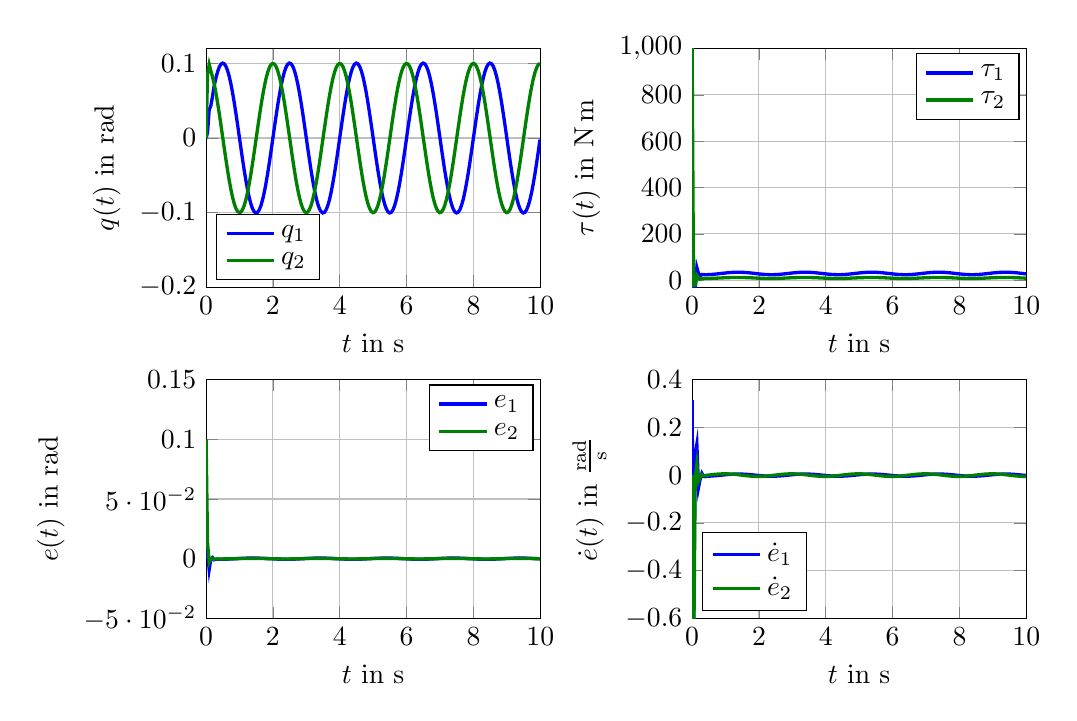
\begin{tikzpicture}

\begin{axis}[%
width=0.35\textwidth,
height=0.25\textwidth,
scale only axis,
xmin=0,
xmax=10,
xlabel={$t$ in $\mathrm{s}$},
xmajorgrids,
ymin=-0.2,
ymax=0.12,
ylabel={$q(t)$ in $\mathrm{rad}$},
ymajorgrids,
name=plot1,
legend style={at={(0.03,0.03)},anchor=south west,draw=black,fill=white,legend cell align=left}
]
\addplot [
color=blue,
solid,
line width=1.2pt
]
table[row sep=crcr]{
0 0\\
0.0428451334891185 0.00719349591461837\\
0.0928451334891186 0.0377668590186034\\
0.142845133489119 0.0434253568614542\\
0.192845133489119 0.0559534941173547\\
0.242845133489119 0.0700083047980907\\
0.292845133489119 0.0802037662270998\\
0.342845133489119 0.0884676832190399\\
0.392845133489119 0.0949253553462922\\
0.442845133489119 0.0989401551180034\\
0.492845133489119 0.100479322144972\\
0.542845133489119 0.099573418628264\\
0.592845133489119 0.0962149494535568\\
0.642845133489119 0.0904821829934969\\
0.692845133489119 0.0825228979734119\\
0.742845133489119 0.0725322442114049\\
0.792845133489119 0.0607553437018495\\
0.842845133489119 0.0474826189616236\\
0.892845133489119 0.0330409399020749\\
0.942845133489119 0.0177857756587457\\
0.992845133489119 0.00209270383800198\\
1.04284513348911 -0.0136519247425698\\
1.09284513348911 -0.0290605009450091\\
1.1428451334891 -0.0437536631103208\\
1.1928451334891 -0.0573696305809554\\
1.24284513348909 -0.0695731120750923\\
1.29284513348909 -0.0800635648319665\\
1.34284513348908 -0.0885826061646672\\
1.39284513348908 -0.0949203918709295\\
1.44284513348907 -0.0989208000873807\\
1.49284513348907 -0.100485289607736\\
1.54284513348906 -0.0995753346235733\\
1.59284513348905 -0.096213374012236\\
1.64284513348905 -0.0904822516498009\\
1.69284513348904 -0.0825231631165929\\
1.74284513348904 -0.0725321623021699\\
1.79284513348903 -0.0607553175977165\\
1.84284513348903 -0.0474826405163814\\
1.89284513348902 -0.0330409389207888\\
1.94284513348902 -0.0177857720523255\\
1.99284513348901 -0.00209270496202322\\
2.042845133489 0.013651924391782\\
2.092845133489 0.029060501238614\\
2.14284513348899 0.0437536630959688\\
2.19284513348899 0.0573696305320419\\
2.24284513348898 0.0695731120904779\\
2.29284513348898 0.0800635648366725\\
2.34284513348897 0.0885826061606427\\
2.39284513348897 0.0949203918711203\\
2.44284513348896 0.0989208000880419\\
2.49284513348896 0.100485289607524\\
2.54284513348895 0.0995753346235134\\
2.59284513348894 0.096213374012301\\
2.64284513348894 0.0904822516498132\\
2.69284513348893 0.0825231631166036\\
2.74284513348893 0.0725321623021969\\
2.79284513348892 0.0607553175977451\\
2.84284513348892 0.0474826405164112\\
2.89284513348891 0.0330409389208216\\
2.94284513348891 0.0177857720523598\\
2.9928451334889 0.00209270496205792\\
3.04284513348889 -0.0136519243917475\\
3.09284513348889 -0.0290605012385807\\
3.14284513348888 -0.0437536630959375\\
3.19284513348888 -0.0573696305320134\\
3.24284513348887 -0.0695731120904528\\
3.29284513348887 -0.0800635648366515\\
3.34284513348886 -0.0885826061606263\\
3.39284513348886 -0.0949203918711089\\
3.44284513348885 -0.0989208000880358\\
3.49284513348884 -0.100485289607523\\
3.54284513348884 -0.0995753346235181\\
3.59284513348883 -0.096213374012311\\
3.64284513348883 -0.0904822516498283\\
3.69284513348882 -0.0825231631166234\\
3.74284513348882 -0.072532162302221\\
3.79284513348881 -0.0607553175977729\\
3.84284513348881 -0.0474826405164419\\
3.8928451334888 -0.0330409389208545\\
3.9428451334888 -0.017785772052394\\
3.99284513348879 -0.0020927049620927\\
4.0428451334888 0.0136519243917152\\
4.09284513348882 0.029060501238557\\
4.14284513348884 0.0437536630959221\\
4.19284513348885 0.0573696305320049\\
4.24284513348887 0.0695731120904504\\
4.29284513348889 0.0800635648366538\\
4.3428451334889 0.0885826061606316\\
4.39284513348892 0.0949203918711149\\
4.44284513348894 0.0989208000880404\\
4.49284513348895 0.100485289607524\\
4.54284513348897 0.0995753346235131\\
4.59284513348899 0.0962133740122981\\
4.642845133489 0.0904822516498058\\
4.69284513348902 0.0825231631165897\\
4.74284513348904 0.0725321623021751\\
4.79284513348905 0.0607553175977144\\
4.84284513348907 0.047482640516371\\
4.89284513348909 0.0330409389207719\\
4.9428451334891 0.0177857720523009\\
4.99284513348912 0.00209270496199108\\
5.04284513348914 -0.0136519243918207\\
5.09284513348915 -0.0290605012386582\\
5.14284513348917 -0.0437536630960168\\
5.19284513348919 -0.0573696305320915\\
5.2428451334892 -0.0695731120905265\\
5.29284513348922 -0.0800635648367176\\
5.34284513348924 -0.0885826061606814\\
5.39284513348925 -0.0949203918711496\\
5.44284513348927 -0.0989208000880591\\
5.49284513348929 -0.100485289607527\\
5.5428451334893 -0.0995753346234988\\
5.59284513348932 -0.0962133740122677\\
5.64284513348934 -0.0904822516497599\\
5.69284513348935 -0.0825231631165295\\
5.74284513348937 -0.072532162302102\\
5.79284513348939 -0.0607553175976304\\
5.8428451334894 -0.0474826405162781\\
5.89284513348942 -0.0330409389206723\\
5.94284513348944 -0.0177857720521972\\
5.99284513348945 -0.00209270496188567\\
6.04284513348947 0.0136519243919252\\
6.09284513348949 0.0290605012387592\\
6.1428451334895 0.0437536630961117\\
6.19284513348952 0.057369630532178\\
6.24284513348954 0.0695731120906026\\
6.29284513348955 0.0800635648367813\\
6.34284513348957 0.0885826061607312\\
6.39284513348959 0.0949203918711842\\
6.4428451334896 0.0989208000880777\\
6.49284513348962 0.100485289607529\\
6.54284513348964 0.0995753346234845\\
6.59284513348965 0.0962133740122372\\
6.64284513348967 0.0904822516497139\\
6.69284513348969 0.0825231631164693\\
6.7428451334897 0.0725321623020291\\
6.79284513348972 0.0607553175975464\\
6.84284513348974 0.0474826405161851\\
6.89284513348975 0.0330409389205727\\
6.94284513348977 0.0177857720520934\\
6.99284513348979 0.00209270496178027\\
7.0428451334898 -0.0136519243920296\\
7.09284513348982 -0.0290605012388601\\
7.14284513348984 -0.0437536630962066\\
7.19284513348985 -0.0573696305322646\\
7.24284513348987 -0.0695731120906787\\
7.29284513348989 -0.080063564836845\\
7.34284513348991 -0.088582606160781\\
7.39284513348992 -0.0949203918712189\\
7.44284513348994 -0.0989208000880964\\
7.49284513348996 -0.100485289607531\\
7.54284513348997 -0.0995753346234702\\
7.59284513348999 -0.0962133740122067\\
7.64284513349001 -0.090482251649668\\
7.69284513349002 -0.0825231631164091\\
7.74284513349004 -0.0725321623019561\\
7.79284513349006 -0.0607553175974624\\
7.84284513349007 -0.0474826405160922\\
7.89284513349009 -0.0330409389204731\\
7.94284513349011 -0.0177857720519896\\
7.99284513349012 -0.00209270496167487\\
8.0428451334901 0.0136519243921294\\
8.09284513349007 0.0290605012389414\\
8.14284513349005 0.0437536630962693\\
8.19284513349002 0.0573696305323107\\
8.24284513348999 0.0695731120907091\\
8.29284513348996 0.0800635648368618\\
8.34284513348993 0.0885826061607873\\
8.39284513348991 0.0949203918712185\\
8.44284513348988 0.0989208000880935\\
8.49284513348985 0.10048528960753\\
8.54284513348982 0.0995753346234752\\
8.5928451334898 0.0962133740122222\\
8.64284513348977 0.0904822516496979\\
8.69284513348974 0.0825231631164564\\
8.74284513348971 0.0725321623020233\\
8.79284513348968 0.0607553175975511\\
8.84284513348966 0.0474826405162028\\
8.89284513348963 0.033040938920605\\
8.9428451334896 0.0177857720521409\\
8.99284513348957 0.00209270496184264\\
9.04284513348955 -0.0136519243919538\\
9.09284513348952 -0.0290605012387733\\
9.14284513348949 -0.0437536630961123\\
9.19284513348946 -0.0573696305321669\\
9.24284513348944 -0.0695731120905827\\
9.29284513348941 -0.080063564836756\\
9.34284513348938 -0.0885826061607046\\
9.39284513348935 -0.094920391871161\\
9.44284513348932 -0.0989208000880624\\
9.4928451334893 -0.100485289607526\\
9.54284513348927 -0.099575334623499\\
9.59284513348924 -0.0962133740122729\\
9.64284513348921 -0.0904822516497741\\
9.69284513348919 -0.0825231631165563\\
9.74284513348916 -0.0725321623021445\\
9.79284513348913 -0.0607553175976905\\
9.8428451334891 -0.047482640516357\\
9.89284513348908 -0.0330409389207703\\
9.94284513348905 -0.0177857720523132\\
9.99284513348902 -0.00209270496201761\\
};
\addlegendentry{$q_1$};

\addplot [
color=green!50!black,
solid,
line width=1.2pt
]
table[row sep=crcr]{
0 0\\
0.0428451334891185 0.0853988885520339\\
0.0928451334891186 0.098708940088748\\
0.142845133489119 0.0900689557848786\\
0.192845133489119 0.0817977227609716\\
0.242845133489119 0.0726646726945513\\
0.292845133489119 0.0608542045158932\\
0.342845133489119 0.0475628655909592\\
0.392845133489119 0.0332544686593849\\
0.442845133489119 0.0180835337013013\\
0.492845133489119 0.0024510178576172\\
0.542845133489119 -0.0132297818378174\\
0.592845133489119 -0.0285850875129798\\
0.642845133489119 -0.0432386342736912\\
0.692845133489119 -0.0568268698315179\\
0.742845133489119 -0.0690155668189786\\
0.792845133489119 -0.0795049822792498\\
0.842845133489119 -0.0880366691889614\\
0.892845133489119 -0.0944005411690932\\
0.942845133489119 -0.0984399597245973\\
0.992845133489119 -0.10005548133459\\
1.04284513348911 -0.0992073427559892\\
1.09284513348911 -0.0959164431165974\\
1.1428451334891 -0.0902638169326873\\
1.1928451334891 -0.0823886396260786\\
1.24284513348909 -0.0724848042485631\\
1.29284513348909 -0.0607961509590149\\
1.34284513348908 -0.0476104682541447\\
1.39284513348908 -0.0332524122275528\\
1.44284513348907 -0.0180755166405895\\
1.49284513348907 -0.0024534897609945\\
1.54284513348906 0.0132289881537118\\
1.59284513348905 0.0285857400422865\\
1.64284513348905 0.0432386059052883\\
1.69284513348904 0.0568267600024587\\
1.74284513348904 0.0690156007223084\\
1.79284513348903 0.0795049931002705\\
1.84284513348903 0.0880366602645163\\
1.89284513348902 0.0944005415726629\\
1.94284513348902 0.0984399612184176\\
1.99284513348901 0.100055480869539\\
2.042845133489 0.0992073426105889\\
2.092845133489 0.095916443238187\\
2.14284513348899 0.0902638169267952\\
2.19284513348899 0.0823886396058503\\
2.24284513348898 0.072484804254968\\
2.29284513348898 0.0607961509610006\\
2.34284513348897 0.047610468252515\\
2.39284513348897 0.0332524122276692\\
2.44284513348896 0.0180755166408999\\
2.49284513348896 0.00245348976094156\\
2.54284513348895 -0.0132289881537043\\
2.59284513348894 -0.0285857400422306\\
2.64284513348894 -0.0432386059052582\\
2.69284513348893 -0.056826760002434\\
2.74284513348893 -0.0690156007222822\\
2.79284513348892 -0.0795049931002491\\
2.84284513348892 -0.0880366602645001\\
2.89284513348891 -0.0944005415726514\\
2.94284513348891 -0.0984399612184113\\
2.9928451334889 -0.100055480869539\\
3.04284513348889 -0.0992073426105935\\
3.09284513348889 -0.0959164432381969\\
3.14284513348888 -0.0902638169268102\\
3.19284513348888 -0.08238863960587\\
3.24284513348887 -0.0724848042549919\\
3.29284513348887 -0.0607961509610281\\
3.34284513348886 -0.0476104682525455\\
3.39284513348886 -0.0332524122277019\\
3.44284513348885 -0.018075516640934\\
3.49284513348884 -0.00245348976097618\\
3.54284513348884 0.0132289881536699\\
3.59284513348883 0.0285857400421974\\
3.64284513348883 0.0432386059052269\\
3.69284513348882 0.0568267600024055\\
3.74284513348882 0.0690156007222571\\
3.79284513348881 0.0795049931002281\\
3.84284513348881 0.0880366602644836\\
3.8928451334888 0.0944005415726399\\
3.9428451334888 0.098439961218405\\
3.99284513348879 0.100055480869538\\
4.0428451334888 0.099207342610597\\
4.09284513348882 0.0959164432382037\\
4.14284513348884 0.0902638169268179\\
4.19284513348885 0.082388639605876\\
4.24284513348887 0.0724848042549944\\
4.29284513348889 0.0607961509610256\\
4.3428451334889 0.0476104682525366\\
4.39284513348892 0.0332524122276857\\
4.44284513348894 0.0180755166409103\\
4.49284513348895 0.0024534897609451\\
4.54284513348897 -0.0132289881537077\\
4.59284513348899 -0.0285857400422405\\
4.642845133489 -0.0432386059052738\\
4.69284513348902 -0.056826760002454\\
4.74284513348904 -0.0690156007223048\\
4.79284513348905 -0.0795049931002723\\
4.84284513348907 -0.0880366602645216\\
4.89284513348909 -0.0944005415726687\\
4.9428451334891 -0.0984399612184218\\
4.99284513348912 -0.10005548086954\\
5.04284513348914 -0.0992073426105837\\
5.09284513348915 -0.0959164432381739\\
5.14284513348917 -0.0902638169267724\\
5.19284513348919 -0.0823886396058164\\
5.2428451334892 -0.0724848042549221\\
5.29284513348922 -0.0607961509609422\\
5.34284513348924 -0.0476104682524442\\
5.39284513348925 -0.0332524122275867\\
5.44284513348927 -0.018075516640807\\
5.49284513348929 -0.00245348976084013\\
5.5428451334893 0.0132289881538117\\
5.59284513348932 0.0285857400423412\\
5.64284513348934 0.0432386059053685\\
5.69284513348935 0.0568267600025405\\
5.74284513348937 0.0690156007223808\\
5.79284513348939 0.0795049931003361\\
5.8428451334894 0.0880366602645715\\
5.89284513348942 0.0944005415727036\\
5.94284513348944 0.0984399612184408\\
5.99284513348945 0.100055480869543\\
6.04284513348947 0.0992073426105698\\
6.09284513348949 0.0959164432381439\\
6.1428451334895 0.090263816926727\\
6.19284513348952 0.0823886396057568\\
6.24284513348954 0.0724848042548496\\
6.29284513348955 0.0607961509608587\\
6.34284513348957 0.0476104682523518\\
6.39284513348959 0.0332524122274877\\
6.4428451334896 0.0180755166407037\\
6.49284513348962 0.00245348976073518\\
6.54284513348964 -0.0132289881539158\\
6.59284513348965 -0.0285857400424418\\
6.64284513348967 -0.0432386059054632\\
6.69284513348969 -0.0568267600026269\\
6.7428451334897 -0.0690156007224569\\
6.79284513348972 -0.0795049931003999\\
6.84284513348974 -0.0880366602646215\\
6.89284513348975 -0.0944005415727384\\
6.94284513348977 -0.0984399612184598\\
6.99284513348979 -0.100055480869545\\
7.0428451334898 -0.0992073426105559\\
7.09284513348982 -0.0959164432381139\\
7.14284513348984 -0.0902638169266817\\
7.19284513348985 -0.0823886396056972\\
7.24284513348987 -0.0724848042547772\\
7.29284513348989 -0.0607961509607754\\
7.34284513348991 -0.0476104682522595\\
7.39284513348992 -0.0332524122273886\\
7.44284513348994 -0.0180755166406005\\
7.49284513348996 -0.00245348976063023\\
7.54284513348997 0.0132289881540199\\
7.59284513348999 0.0285857400425424\\
7.64284513349001 0.0432386059055579\\
7.69284513349002 0.0568267600027133\\
7.74284513349004 0.0690156007225329\\
7.79284513349006 0.0795049931004636\\
7.84284513349007 0.0880366602646714\\
7.89284513349009 0.0944005415727733\\
7.94284513349011 0.0984399612184787\\
7.99284513349012 0.100055480869548\\
8.0428451334901 0.0992073426105442\\
8.09284513349007 0.0959164432380901\\
8.14284513349005 0.090263816926651\\
8.19284513349002 0.0823886396056651\\
8.24284513348999 0.0724848042547478\\
8.29284513348996 0.0607961509607525\\
8.34284513348993 0.0476104682522464\\
8.39284513348991 0.0332524122273877\\
8.44284513348988 0.0180755166406132\\
8.49284513348985 0.00245348976065707\\
8.54284513348982 -0.0132289881539794\\
8.5928451334898 -0.02858574004249\\
8.64284513348977 -0.043238605905496\\
8.69284513348974 -0.0568267600026453\\
8.74284513348971 -0.069015600722463\\
8.79284513348968 -0.0795049931003966\\
8.84284513348966 -0.0880366602646123\\
8.89284513348963 -0.0944005415727275\\
8.9428451334896 -0.0984399612184514\\
8.99284513348957 -0.100055480869544\\
9.04284513348955 -0.0992073426105661\\
9.09284513348952 -0.0959164432381396\\
9.14284513348949 -0.0902638169267265\\
9.19284513348946 -0.082388639605764\\
9.24284513348944 -0.072484804254868\\
9.29284513348941 -0.0607961509608909\\
9.34284513348938 -0.0476104682523997\\
9.39284513348935 -0.0332524122275521\\
9.44284513348932 -0.0180755166407846\\
9.4928451334893 -0.0024534897608313\\
9.54284513348927 0.0132289881538067\\
9.59284513348924 0.0285857400423229\\
9.64284513348921 0.0432386059053388\\
9.69284513348919 0.0568267600025019\\
9.74284513348916 0.0690156007223368\\
9.79284513348913 0.0795049931002907\\
9.8428451334891 0.0880366602645294\\
9.89284513348908 0.0944005415726696\\
9.94284513348905 0.0984399612184199\\
9.99284513348902 0.10005548086954\\
};
\addlegendentry{$q_2$};

\end{axis}

\begin{axis}[%
width=0.35\textwidth,
height=0.25\textwidth,
scale only axis,
xmin=0,
xmax=10,
xlabel={$t$ in $\mathrm{s}$},
xmajorgrids,
ymin=-0.05,
ymax=0.15,
ylabel={$e(t)$ in $\mathrm{rad}$},
ymajorgrids,
name=plot3,
at=(plot1.below south west),
anchor=above north west,
legend style={draw=black,fill=white,legend cell align=left}
]
\addplot [
color=blue,
solid,
line width=1.2pt
]
table[row sep=crcr]{
0 0\\
0.0428451334891185 0.00622609194858809\\
0.0928451334891186 -0.00901053975009558\\
0.142845133489119 -4.03822047876784e-05\\
0.192845133489119 0.000991853864947517\\
0.242845133489119 -0.000904766948251645\\
0.292845133489119 -0.00064359695308043\\
0.342845133489119 -0.000409917933430023\\
0.392845133489119 -0.000538268477391232\\
0.442845133489119 -0.000547869997305536\\
0.492845133489119 -0.00050458337742143\\
0.542845133489119 -0.000477936079453178\\
0.592845133489119 -0.000438782782888489\\
0.642845133489119 -0.000383659287276253\\
0.692845133489119 -0.000320541905142802\\
0.742845133489119 -0.00025015060146677\\
0.792845133489119 -0.000173337585434225\\
0.842845133489119 -9.24303894684619e-05\\
0.892845133489119 -9.47259584493237e-06\\
0.942845133489119 7.362603132487e-05\\
0.992845133489119 0.000154874494343495\\
1.04284513348911 0.000232336879364503\\
1.09284513348911 0.000304181676504128\\
1.1428451334891 0.00036868845365854\\
1.1928451334891 0.000424282598658503\\
1.24284513348909 0.000469574225259214\\
1.29284513348909 0.000503395557953173\\
1.34284513348908 0.000524840879062835\\
1.39284513348908 0.000533305002033024\\
1.44284513348907 0.000528514966685587\\
1.49284513348907 0.000510550840186072\\
1.54284513348906 0.000479852074759896\\
1.59284513348905 0.000437207341561816\\
1.64284513348905 0.000383727943570694\\
1.69284513348904 0.000320807048310154\\
1.74284513348904 0.000250068692214098\\
1.79284513348903 0.000173311481279498\\
1.84284513348903 9.24519442005584e-05\\
1.89284513348902 9.47161452965334e-06\\
1.94284513348902 -7.36296377771145e-05\\
1.99284513348901 -0.000154873370356638\\
2.042845133489 -0.000232336528610993\\
2.092845133489 -0.000304181970142255\\
2.14284513348899 -0.000368688439337787\\
2.19284513348899 -0.000424282549773398\\
2.24284513348898 -0.000469574240669804\\
2.29284513348898 -0.000503395562680128\\
2.34284513348897 -0.000524840875054791\\
2.39284513348897 -0.000533305002235265\\
2.44284513348896 -0.000528514967352969\\
2.49284513348896 -0.000510550839974783\\
2.54284513348895 -0.000479852074695364\\
2.59284513348894 -0.000437207341616869\\
2.64284513348894 -0.000383727943568044\\
2.69284513348893 -0.000320807048301119\\
2.74284513348893 -0.000250068692217151\\
2.79284513348892 -0.000173311481280629\\
2.84284513348892 -9.24519441999755e-05\\
2.89284513348891 -9.47161452979906e-06\\
2.94284513348891 7.36296377768682e-05\\
2.9928451334889 0.000154873370356488\\
3.04284513348889 0.000232336528610809\\
3.09284513348889 0.000304181970142113\\
3.14284513348888 0.00036868843933769\\
3.19284513348888 0.000424282549773343\\
3.24284513348887 0.000469574240669679\\
3.29284513348887 0.000503395562680004\\
3.34284513348886 0.000524840875054777\\
3.39284513348886 0.000533305002235265\\
3.44284513348885 0.000528514967353011\\
3.49284513348884 0.00051055083997481\\
3.54284513348884 0.000479852074695447\\
3.59284513348883 0.000437207341616924\\
3.64284513348883 0.000383727943568099\\
3.69284513348882 0.000320807048301314\\
3.74284513348882 0.000250068692217276\\
3.79284513348881 0.000173311481280788\\
3.84284513348881 9.2451944200142e-05\\
3.8928451334888 9.47161453011824e-06\\
3.9428451334888 -7.36296377767363e-05\\
3.99284513348879 -0.000154873370356349\\
4.0428451334888 -0.000232336528607041\\
4.09284513348882 -0.000304181970139154\\
4.14284513348884 -0.000368688439335567\\
4.19284513348885 -0.000424282549771275\\
4.24284513348887 -0.000469574240667972\\
4.29284513348889 -0.000503395562678713\\
4.3428451334889 -0.000524840875053806\\
4.39284513348892 -0.000533305002234641\\
4.44284513348894 -0.000528514967352775\\
4.49284513348895 -0.000510550839975019\\
4.54284513348897 -0.000479852074695961\\
4.59284513348899 -0.000437207341617826\\
4.642845133489 -0.00038372794356932\\
4.69284513348902 -0.000320807048302785\\
4.74284513348904 -0.00025006869221901\\
4.79284513348905 -0.000173311481282634\\
4.84284513348907 -9.24519442020919e-05\\
4.89284513348909 -9.47161453212358e-06\\
4.9428451334891 7.36296377745714e-05\\
4.99284513348912 0.000154873370354266\\
5.04284513348914 0.00023233652860853\\
5.09284513348915 0.000304181970139848\\
5.14284513348917 0.00036868843933565\\
5.19284513348919 0.000424282549771726\\
5.2428451334892 0.000469574240668208\\
5.29284513348922 0.000503395562678949\\
5.34284513348924 0.000524840875053847\\
5.39284513348925 0.000533305002234696\\
5.44284513348927 0.000528514967352692\\
5.49284513348929 0.000510550839974838\\
5.5428451334893 0.000479852074695739\\
5.59284513348932 0.000437207341617479\\
5.64284513348934 0.000383727943568987\\
5.69284513348935 0.000320807048302257\\
5.74284513348937 0.000250068692218539\\
5.79284513348939 0.00017331148128201\\
5.8428451334894 9.245194420162e-05\\
5.89284513348942 9.47161453181827e-06\\
5.94284513348944 -7.3629637775071e-05\\
5.99284513348945 -0.000154873370354559\\
6.04284513348947 -0.000232336528609137\\
6.09284513348949 -0.000304181970140243\\
6.1428451334895 -0.000368688439336164\\
6.19284513348952 -0.000424282549771844\\
6.24284513348954 -0.000469574240668527\\
6.29284513348955 -0.00050339556267899\\
6.34284513348957 -0.000524840875054014\\
6.39284513348959 -0.000533305002234627\\
6.4428451334896 -0.00052851496735265\\
6.49284513348962 -0.000510550839974686\\
6.54284513348964 -0.000479852074695489\\
6.59284513348965 -0.000437207341617271\\
6.64284513348967 -0.000383727943568501\\
6.69284513348969 -0.000320807048301952\\
6.7428451334897 -0.000250068692217956\\
6.79284513348972 -0.00017331148128167\\
6.84284513348974 -9.24519442009886e-05\\
6.89284513348975 -9.47161453112438e-06\\
6.94284513348977 7.36296377757267e-05\\
6.99284513348979 0.000154873370355195\\
7.0428451334898 0.000232336528609737\\
7.09284513348982 0.000304181970140812\\
7.14284513348984 0.00036868843933667\\
7.19284513348985 0.000424282549772267\\
7.24284513348987 0.000469574240668943\\
7.29284513348989 0.000503395562679226\\
7.34284513348991 0.000524840875054153\\
7.39284513348992 0.000533305002234655\\
7.44284513348994 0.000528514967352525\\
7.49284513348996 0.000510550839974533\\
7.54284513348997 0.000479852074695253\\
7.59284513348999 0.000437207341616855\\
7.64284513349001 0.000383727943568224\\
7.69284513349002 0.000320807048301425\\
7.74284513349004 0.00025006869221765\\
7.79284513349006 0.000173311481281052\\
7.84284513349007 9.24519442006486e-05\\
7.89284513349009 9.47161453046519e-06\\
7.94284513349011 -7.3629637776032e-05\\
7.99284513349012 -0.000154873370355826\\
8.0428451334901 -0.000232336528617297\\
8.09284513349007 -0.000304181970146589\\
8.14284513349005 -0.000368688439340792\\
8.19284513349002 -0.000424282549776368\\
8.24284513348999 -0.000469574240672316\\
8.29284513348996 -0.000503395562682002\\
8.34284513348993 -0.000524840875056137\\
8.39284513348991 -0.000533305002235834\\
8.44284513348988 -0.000528514967352955\\
8.49284513348985 -0.000510550839974144\\
8.54284513348982 -0.000479852074694045\\
8.5928451334898 -0.000437207341615023\\
8.64284513348977 -0.000383727943565712\\
8.69284513348974 -0.000320807048298358\\
8.74284513348971 -0.000250068692213917\\
8.79284513348968 -0.000173311481277305\\
8.84284513348966 -9.24519441963881e-05\\
8.89284513348963 -9.4716145261492e-06\\
8.9428451334896 7.36296377806533e-05\\
8.99284513348957 0.000154873370359977\\
9.04284513348955 0.000232336528614248\\
9.09284513348952 0.000304181970145274\\
9.14284513348949 0.000368688439340653\\
9.19284513348946 0.000424282549775709\\
9.24284513348944 0.000469574240671719\\
9.29284513348941 0.000503395562681697\\
9.34284513348938 0.000524840875055929\\
9.39284513348935 0.000533305002235807\\
9.44284513348932 0.000528514967353053\\
9.4928451334893 0.000510550839974366\\
9.54284513348927 0.00047985207469449\\
9.59284513348924 0.000437207341615606\\
9.64284513348921 0.00038372794356635\\
9.69284513348919 0.000320807048299079\\
9.74284513348916 0.000250068692214764\\
9.79284513348913 0.000173311481278186\\
9.8428451334891 9.24519441973318e-05\\
9.89284513348908 9.4716145271137e-06\\
9.94284513348905 -7.36296377797166e-05\\
9.99284513348902 -0.000154873370359411\\
};
\addlegendentry{$e_1$};

\addplot [
color=green!50!black,
solid,
line width=1.2pt
]
table[row sep=crcr]{
0 0.1\\
0.0428451334891185 0.0136965939967769\\
0.0928451334891186 -0.00293277341807961\\
0.142845133489119 2.95679213420524e-05\\
0.192845133489119 0.000404633307297592\\
0.242845133489119 -0.000382579084613116\\
0.292845133489119 -0.000272198399477876\\
0.342845133489119 -0.000172677018803954\\
0.392845133489119 -0.000223001353154791\\
0.442845133489119 -0.000224132011230636\\
0.492845133489119 -0.000203439525271596\\
0.542845133489119 -0.000189806025389191\\
0.592845133489119 -0.000171231755528096\\
0.642845133489119 -0.000146340382975382\\
0.692845133489119 -0.00011847815078446\\
0.742845133489119 -8.79710308605286e-05\\
0.792845133489119 -5.51869947696404e-05\\
0.842845133489119 -2.10960966485485e-05\\
0.892845133489119 1.34543001922144e-05\\
0.942845133489119 4.76746038994003e-05\\
0.992845133489119 8.0742567039549e-05\\
1.04284513348911 0.000111860207178141\\
1.09284513348911 0.000140276445928192\\
1.1428451334891 0.000165293226464608\\
1.1928451334891 0.000186283557805755\\
1.24284513348909 0.000202710638619263\\
1.29284513348909 0.000214144842591697\\
1.34284513348908 0.000220279681979171\\
1.39284513348908 0.000220944921310008\\
1.44284513348907 0.000216114950503929\\
1.49284513348907 0.000205911428631964\\
1.54284513348906 0.000190599709476307\\
1.59284513348905 0.000170579226201856\\
1.64284513348905 0.000146368751358393\\
1.69284513348904 0.000118587979823948\\
1.74284513348904 8.79371275121776e-05\\
1.79284513348903 5.51761737323381e-05\\
1.84284513348903 2.11050210798813e-05\\
1.89284513348902 -1.34547037721339e-05\\
1.94284513348902 -4.76760977255186e-05\\
1.99284513348901 -8.07421019895643e-05\\
2.042845133489 -0.000111860061773175\\
2.092845133489 -0.000140276567507855\\
2.14284513348899 -0.0001652932205575\\
2.19284513348899 -0.000186283537557771\\
2.24284513348898 -0.000202710645000215\\
2.29284513348898 -0.000214144844549881\\
2.34284513348897 -0.000220279680318985\\
2.39284513348897 -0.000220944921393823\\
2.44284513348896 -0.000216114950780298\\
2.49284513348896 -0.000205911428544469\\
2.54284513348895 -0.000190599709449518\\
2.59284513348894 -0.000170579226224682\\
2.64284513348894 -0.000146368751357318\\
2.69284513348893 -0.000118587979820166\\
2.74284513348893 -8.79371275133989e-05\\
2.79284513348892 -5.5176173732796e-05\\
2.84284513348892 -2.11050210796732e-05\\
2.89284513348891 1.34547037720784e-05\\
2.94284513348891 4.76760977253798e-05\\
2.9928451334889 8.07421019895227e-05\\
3.04284513348889 0.000111860061773134\\
3.09284513348889 0.000140276567507716\\
3.14284513348888 0.00016529322055743\\
3.19284513348888 0.000186283537557744\\
3.24284513348887 0.000202710645000229\\
3.29284513348887 0.000214144844549902\\
3.34284513348886 0.000220279680318951\\
3.39284513348886 0.000220944921393795\\
3.44284513348885 0.000216114950780368\\
3.49284513348884 0.000205911428544538\\
3.54284513348884 0.000190599709449518\\
3.59284513348883 0.000170579226224696\\
3.64284513348883 0.000146368751357352\\
3.69284513348882 0.000118587979820346\\
3.74284513348882 8.79371275134405e-05\\
3.79284513348881 5.51761737328516e-05\\
3.84284513348881 2.11050210797287e-05\\
3.8928451334888 -1.34547037719535e-05\\
3.9428451334888 -4.76760977253105e-05\\
3.99284513348879 -8.07421019894672e-05\\
4.0428451334888 -0.000111860061772787\\
4.09284513348882 -0.000140276567508354\\
4.14284513348884 -0.000165293220558707\\
4.19284513348885 -0.00018628353755927\\
4.24284513348887 -0.000202710645002144\\
4.29284513348889 -0.000214144844552157\\
4.3428451334889 -0.000220279680321546\\
4.39284513348892 -0.000220944921396543\\
4.44284513348894 -0.000216114950783195\\
4.49284513348895 -0.000205911428547372\\
4.54284513348897 -0.000190599709452441\\
4.59284513348899 -0.000170579226227471\\
4.642845133489 -0.000146368751359899\\
4.69284513348902 -0.000118587979822622\\
4.74284513348904 -8.79371275155222e-05\\
4.79284513348905 -5.51761737345724e-05\\
4.84284513348907 -2.11050210809915e-05\\
4.89284513348909 1.34547037711347e-05\\
4.9428451334891 4.76760977248664e-05\\
4.99284513348912 8.07421019894811e-05\\
5.04284513348914 0.000111860061773578\\
5.09284513348915 0.00014027656750866\\
5.14284513348917 0.000165293220558763\\
5.19284513348919 0.000186283537559381\\
5.2428451334892 0.000202710645002324\\
5.29284513348922 0.000214144844552094\\
5.34284513348924 0.000220279680321622\\
5.39284513348925 0.000220944921396418\\
5.44284513348927 0.000216114950783219\\
5.49284513348929 0.000205911428547168\\
5.5428451334893 0.000190599709452398\\
5.59284513348932 0.000170579226227211\\
5.64284513348934 0.000146368751359802\\
5.69284513348935 0.000118587979822338\\
5.74284513348937 8.79371275153557e-05\\
5.79284513348939 5.51761737342393e-05\\
5.8428451334894 2.11050210807973e-05\\
5.89284513348942 -1.34547037712596e-05\\
5.94284513348944 -4.76760977250884e-05\\
5.99284513348945 -8.07421019896892e-05\\
6.04284513348947 -0.000111860061773744\\
6.09284513348949 -0.000140276567508854\\
6.1428451334895 -0.000165293220558888\\
6.19284513348952 -0.000186283537559631\\
6.24284513348954 -0.000202710645002338\\
6.29284513348955 -0.000214144844552323\\
6.34284513348957 -0.000220279680321539\\
6.39284513348959 -0.00022094492139664\\
6.4428451334896 -0.000216114950783056\\
6.49284513348962 -0.000205911428547337\\
6.54284513348964 -0.000190599709452158\\
6.59284513348965 -0.000170579226227305\\
6.64284513348967 -0.000146368751359517\\
6.69284513348969 -0.000118587979822345\\
6.7428451334897 -8.79371275150503e-05\\
6.79284513348972 -5.51761737341699e-05\\
6.84284513348974 -2.11050210805475e-05\\
6.89284513348975 1.34547037715094e-05\\
6.94284513348977 4.76760977253521e-05\\
6.99284513348979 8.07421019899252e-05\\
7.0428451334898 0.000111860061773911\\
7.09284513348982 0.000140276567509035\\
7.14284513348984 0.000165293220559012\\
7.19284513348985 0.000186283537559714\\
7.24284513348987 0.000202710645002324\\
7.29284513348989 0.000214144844552323\\
7.34284513348991 0.000220279680321483\\
7.39284513348992 0.000220944921396508\\
7.44284513348994 0.000216114950783251\\
7.49284513348996 0.000205911428547149\\
7.54284513348997 0.000190599709452288\\
7.59284513348999 0.000170579226227048\\
7.64284513349001 0.000146368751359552\\
7.69284513349002 0.000118587979822074\\
7.74284513349004 8.79371275150365e-05\\
7.79284513349006 5.51761737338924e-05\\
7.84284513349007 2.11050210804087e-05\\
7.89284513349009 -1.34547037718286e-05\\
7.94284513349011 -4.76760977255186e-05\\
7.99284513349012 -8.07421019901056e-05\\
8.0428451334901 -0.000111860061774674\\
8.09284513349007 -0.000140276567507897\\
8.14284513349005 -0.000165293220556528\\
8.19284513349002 -0.000186283537556703\\
8.24284513348999 -0.000202710644998688\\
8.29284513348996 -0.000214144844547785\\
8.34284513348993 -0.000220279680316474\\
8.39284513348991 -0.000220944921391228\\
8.44284513348988 -0.000216114950777446\\
8.49284513348985 -0.000205911428541307\\
8.54284513348982 -0.000190599709446239\\
8.5928451334898 -0.00017057922622165\\
8.64284513348977 -0.000146368751354257\\
8.69284513348974 -0.000118587979817328\\
8.74284513348971 -8.79371275106788e-05\\
8.79284513348968 -5.51761737305756e-05\\
8.84284513348966 -2.11050210777025e-05\\
8.89284513348963 1.3454703773591e-05\\
8.9428451334896 4.76760977264623e-05\\
8.99284513348957 8.07421019901333e-05\\
9.04284513348955 0.000111860061773258\\
9.09284513348952 0.000140276567507369\\
9.14284513348949 0.000165293220556501\\
9.19284513348946 0.000186283537556509\\
9.24284513348944 0.000202710644998522\\
9.29284513348941 0.000214144844547702\\
9.34284513348938 0.00022027968031646\\
9.39284513348935 0.000220944921391283\\
9.44284513348932 0.000216114950777564\\
9.4928451334893 0.000205911428541486\\
9.54284513348927 0.000190599709446475\\
9.59284513348924 0.000170579226221924\\
9.64284513348921 0.00014636875135457\\
9.69284513348919 0.000118587979817661\\
9.74284513348916 8.79371275110674e-05\\
9.79284513348913 5.51761737309364e-05\\
9.8428451334891 2.1105021078105e-05\\
9.89284513348908 -1.34547037731747e-05\\
9.94284513348905 -4.76760977261015e-05\\
9.99284513348902 -8.07421019897725e-05\\
};
\addlegendentry{$e_2$};

\end{axis}

\begin{axis}[%
width=0.35\textwidth,
height=0.25\textwidth,
scale only axis,
xmin=0,
xmax=10,
xlabel={$t$ in $\mathrm{s}$},
xmajorgrids,
ymin=-0.6,
ymax=0.4,
ylabel={$\dot{e}(t)$ in $\mathrm{\frac{rad}{s}}$},
ymajorgrids,
name=plot2,
at=(plot3.right of south east),
anchor=left of south west,
legend style={at={(0.03,0.03)},anchor=south west,draw=black,fill=white,legend cell align=left}
]
\addplot [
color=blue,
solid,
line width=1.2pt
]
table[row sep=crcr]{
0 0.314159265358979\\
0.0428451334891185 -0.635734068331703\\
0.0928451334891186 0.0860425636544677\\
0.142845133489119 0.128930016739003\\
0.192845133489119 -0.051364473427748\\
0.242845133489119 -0.0151178226720267\\
0.292845133489119 0.00705922377655732\\
0.342845133489119 -0.00555676916405765\\
0.392845133489119 -0.00634883576668065\\
0.442845133489119 -0.00383104033909929\\
0.492845133489119 -0.00414371530043279\\
0.542845133489119 -0.00415454706451788\\
0.592845133489119 -0.00359057962968987\\
0.642845133489119 -0.00309975459741593\\
0.692845133489119 -0.00257732867833366\\
0.742845133489119 -0.00195268413355792\\
0.792845133489119 -0.0012835977847811\\
0.842845133489119 -0.000589562456681958\\
0.892845133489119 0.000121740766335643\\
0.942845133489119 0.000831784740045471\\
0.992845133489119 0.00152230598374303\\
1.04284513348911 0.00217691540797776\\
1.09284513348911 0.00277923539973535\\
1.1428451334891 0.0033137429951946\\
1.1928451334891 0.00376658348611214\\
1.24284513348909 0.0041259191038687\\
1.29284513348909 0.00438235709050758\\
1.34284513348908 0.00452932900353445\\
1.39284513348908 0.00456330337265187\\
1.44284513348907 0.00448385062810945\\
1.49284513348907 0.0042935672681821\\
1.54284513348906 0.00399787223571618\\
1.59284513348905 0.00360471236427405\\
1.64284513348905 0.00312422078733238\\
1.69284513348904 0.00256836853565956\\
1.74284513348904 0.00195063961311956\\
1.79284513348903 0.00128574403491594\\
1.84284513348903 0.000589365569959144\\
1.89284513348902 -0.000122074075289857\\
1.94284513348902 -0.000831661806919681\\
1.99284513348901 -0.00152227856172027\\
2.042845133489 -0.00217694464836132\\
2.092845133489 -0.00277923262640462\\
2.14284513348899 -0.00331373848397792\\
2.19284513348899 -0.00376658516842865\\
2.24284513348898 -0.00412591947106583\\
2.29284513348898 -0.00438235669228801\\
2.34284513348897 -0.00452932904209372\\
2.39284513348897 -0.00456330343406718\\
2.44284513348896 -0.00448385060507699\\
2.49284513348896 -0.00429356726318058\\
2.54284513348895 -0.00399787224116913\\
2.59284513348894 -0.00360471236374356\\
2.64284513348894 -0.00312422078649047\\
2.69284513348893 -0.00256836853597722\\
2.74284513348893 -0.00195063961318837\\
2.79284513348892 -0.00128574403484066\\
2.84284513348892 -0.00058936556996847\\
2.89284513348891 0.000122074075275591\\
2.94284513348891 0.000831661806922068\\
2.9928451334889 0.00152227856172044\\
3.04284513348889 0.00217694464835755\\
3.09284513348889 0.00277923262640223\\
3.14284513348888 0.0033137384839787\\
3.19284513348888 0.00376658516842893\\
3.24284513348887 0.00412591947106486\\
3.29284513348887 0.00438235669228787\\
3.34284513348886 0.00452932904209474\\
3.39284513348886 0.00456330343406894\\
3.44284513348885 0.00448385060507586\\
3.49284513348884 0.00429356726317936\\
3.54284513348884 0.00399787224117074\\
3.59284513348883 0.00360471236374739\\
3.64284513348883 0.00312422078649377\\
3.69284513348882 0.00256836853597917\\
3.74284513348882 0.00195063961319011\\
3.79284513348881 0.00128574403484177\\
3.84284513348881 0.000589365569969635\\
3.8928451334888 -0.000122074075274869\\
3.9428451334888 -0.000831661806919959\\
3.99284513348879 -0.00152227856171849\\
4.0428451334888 -0.00217694464847368\\
4.09284513348882 -0.00277923262656821\\
4.14284513348884 -0.00331373848410682\\
4.19284513348885 -0.00376658516854494\\
4.24284513348887 -0.0041259194711771\\
4.29284513348889 -0.00438235669238246\\
4.3428451334889 -0.00452932904217002\\
4.39284513348892 -0.0045633034341237\\
4.44284513348894 -0.00448385060511444\\
4.49284513348895 -0.00429356726319451\\
4.54284513348897 -0.00399787224116328\\
4.59284513348899 -0.00360471236371489\\
4.642845133489 -0.00312422078644026\\
4.69284513348902 -0.00256836853590384\\
4.74284513348904 -0.00195063961309694\\
4.79284513348905 -0.00128574403473358\\
4.84284513348907 -0.000589365569847178\\
4.89284513348909 0.000122074075408596\\
4.9428451334891 0.000831661807061734\\
4.99284513348912 0.00152227856186388\\
5.04284513348914 0.00217694464850277\\
5.09284513348915 0.00277923262654484\\
5.14284513348917 0.00331373848411315\\
5.19284513348919 0.00376658516855188\\
5.2428451334892 0.00412591947117799\\
5.29284513348922 0.00438235669238418\\
5.34284513348924 0.0045293290421711\\
5.39284513348925 0.00456330343412391\\
5.44284513348927 0.00448385060511269\\
5.49284513348929 0.00429356726319281\\
5.5428451334893 0.00399787224116074\\
5.59284513348932 0.00360471236371213\\
5.64284513348934 0.00312422078643562\\
5.69284513348935 0.00256836853590039\\
5.74284513348937 0.00195063961309347\\
5.79284513348939 0.00128574403472975\\
5.8428451334894 0.000589365569841738\\
5.89284513348942 -0.000122074075414591\\
5.94284513348944 -0.000831661807066786\\
5.99284513348945 -0.00152227856186804\\
6.04284513348947 -0.0021769446485066\\
6.09284513348949 -0.00277923262655133\\
6.1428451334895 -0.00331373848411504\\
6.19284513348952 -0.00376658516855832\\
6.24284513348954 -0.00412591947118068\\
6.29284513348955 -0.00438235669238915\\
6.34284513348957 -0.00452932904217179\\
6.39284513348959 -0.00456330343412482\\
6.4428451334896 -0.00448385060511165\\
6.49284513348962 -0.0042935672631918\\
6.54284513348964 -0.00399787224115763\\
6.59284513348965 -0.00360471236370831\\
6.64284513348967 -0.0031242207864324\\
6.69284513348969 -0.00256836853589648\\
6.7428451334897 -0.0019506396130885\\
6.79284513348972 -0.00128574403472537\\
6.84284513348974 -0.000589365569837352\\
6.89284513348975 0.000122074075418088\\
6.94284513348977 0.000831661807071671\\
6.99284513348979 0.00152227856187259\\
7.0428451334898 0.00217694464851126\\
7.09284513348982 0.00277923262655227\\
7.14284513348984 0.0033137384841192\\
7.19284513348985 0.00376658516855649\\
7.24284513348987 0.00412591947118218\\
7.29284513348989 0.00438235669238607\\
7.34284513348991 0.00452932904217401\\
7.39284513348992 0.00456330343412331\\
7.44284513348994 0.00448385060511274\\
7.49284513348996 0.0042935672631882\\
7.54284513348997 0.00399787224115584\\
7.59284513348999 0.00360471236370584\\
7.64284513349001 0.0031242207864299\\
7.69284513349002 0.00256836853589282\\
7.74284513349004 0.0019506396130852\\
7.79284513349006 0.00128574403472087\\
7.84284513349007 0.000589365569832245\\
7.89284513349009 -0.000122074075423972\\
7.94284513349011 -0.000831661807076389\\
7.99284513349012 -0.00152227856187742\\
8.0428451334901 -0.002176944648276\\
8.09284513349007 -0.00277923262622587\\
8.14284513349005 -0.00331373848386513\\
8.19284513349002 -0.00376658516832251\\
8.24284513348999 -0.00412591947096408\\
8.29284513348996 -0.00438235669219927\\
8.34284513348993 -0.00452932904202047\\
8.39284513348991 -0.00456330343401021\\
8.44284513348988 -0.00448385060504368\\
8.49284513348985 -0.00429356726316372\\
8.54284513348982 -0.00399787224117474\\
8.5928451334898 -0.00360471236377126\\
8.64284513348977 -0.0031242207865394\\
8.69284513348974 -0.00256836853604062\\
8.74284513348971 -0.00195063961326974\\
8.79284513348968 -0.00128574403493892\\
8.84284513348966 -0.000589365570077993\\
8.89284513348963 0.00012207407515602\\
8.9428451334896 0.000831661806794726\\
8.99284513348957 0.00152227856158799\\
9.04284513348955 0.00217694464822654\\
9.09284513348952 0.00277923262627428\\
9.14284513348949 0.00331373848385297\\
9.19284513348946 0.00376658516831091\\
9.24284513348944 0.00412591947096461\\
9.29284513348941 0.00438235669220013\\
9.34284513348938 0.00452932904202011\\
9.39284513348935 0.00456330343401105\\
9.44284513348932 0.00448385060504168\\
9.4928451334893 0.00429356726316889\\
9.54284513348927 0.00399787224117839\\
9.59284513348924 0.00360471236377469\\
9.64284513348921 0.00312422078654118\\
9.69284513348919 0.00256836853604994\\
9.74284513348916 0.00195063961327727\\
9.79284513348913 0.00128574403494663\\
9.8428451334891 0.000589365570086986\\
9.89284513348908 -0.000122074075148693\\
9.94284513348905 -0.000831661806787287\\
9.99284513348902 -0.0015222785615796\\
};
\addlegendentry{$\dot{e}_1$};

\addplot [
color=green!50!black,
solid,
line width=1.2pt
]
table[row sep=crcr]{
0 -0\\
0.0428451334891185 -0.850080042746216\\
0.0928451334891186 -0.0109601972396559\\
0.142845133489119 0.0469179074312743\\
0.192845133489119 -0.0242198661208735\\
0.242845133489119 -0.00828392992892824\\
0.292845133489119 0.00169276378020805\\
0.342845133489119 -0.00272835748818595\\
0.392845133489119 -0.00224321388034815\\
0.442845133489119 -0.000396946312429258\\
0.492845133489119 0.000247216161095576\\
0.542845133489119 0.000967829471195669\\
0.592845133489119 0.00186021991904395\\
0.642845133489119 0.00263997457472087\\
0.692845133489119 0.00333643473383488\\
0.742845133489119 0.00396713342583874\\
0.792845133489119 0.00449901723899981\\
0.842845133489119 0.00491768614996069\\
0.892845133489119 0.00521660610098459\\
0.942845133489119 0.00538783351269458\\
0.992845133489119 0.00542665636389283\\
1.04284513348911 0.00533222969165867\\
1.09284513348911 0.00510668883135539\\
1.1428451334891 0.00475529657213755\\
1.1928451334891 0.00428649326630604\\
1.24284513348909 0.00371167599942002\\
1.29284513348909 0.00304494462677754\\
1.34284513348908 0.00230277865201062\\
1.39284513348908 0.00150361595868553\\
1.44284513348907 0.000667361769428387\\
1.49284513348907 -0.000185150313633087\\
1.54284513348906 -0.00103272432402157\\
1.59284513348905 -0.0018543688385268\\
1.64284513348905 -0.00262984040806641\\
1.69284513348904 -0.00334014446668296\\
1.74284513348904 -0.0039679809397335\\
1.79284513348903 -0.00449812852296325\\
1.84284513348903 -0.00491776744233555\\
1.89284513348902 -0.00521674417373814\\
1.94284513348902 -0.00538778264183613\\
1.99284513348901 -0.00542664498999036\\
2.042845133489 -0.0053322417991257\\
2.092845133489 -0.00510668768588039\\
2.14284513348899 -0.00475529470336322\\
2.19284513348899 -0.00428649396281619\\
2.24284513348898 -0.00371167615159879\\
2.29284513348898 -0.00304494446183862\\
2.34284513348897 -0.00230277866798456\\
2.39284513348897 -0.00150361598412363\\
2.44284513348896 -0.000667361759892182\\
2.49284513348896 0.000185150315704652\\
2.54284513348895 0.00103272432175944\\
2.59284513348894 0.0018543688387434\\
2.64284513348894 0.00262984040841185\\
2.69284513348893 0.00334014446654884\\
2.74284513348893 0.00396798093970407\\
2.79284513348892 0.00449812852299328\\
2.84284513348892 0.00491776744233266\\
2.89284513348891 0.0052167441737314\\
2.94284513348891 0.00538778264183829\\
2.9928451334889 0.00542664498999035\\
3.04284513348889 0.00533224179912711\\
3.09284513348889 0.00510668768588575\\
3.14284513348888 0.00475529470336158\\
3.19284513348888 0.00428649396281278\\
3.24284513348887 0.00371167615160076\\
3.29284513348887 0.00304494446184211\\
3.34284513348886 0.00230277866798523\\
3.39284513348886 0.00150361598412274\\
3.44284513348885 0.000667361759894902\\
3.49284513348884 -0.000185150315700378\\
3.54284513348884 -0.00103272432175738\\
3.59284513348883 -0.00185436883874635\\
3.64284513348883 -0.0026298404084118\\
3.69284513348882 -0.00334014446654762\\
3.74284513348882 -0.00396798093970169\\
3.79284513348881 -0.00449812852299189\\
3.84284513348881 -0.00491776744233208\\
3.8928451334888 -0.00521674417373168\\
3.9428451334888 -0.00538778264183895\\
3.99284513348879 -0.00542664498998991\\
4.0428451334888 -0.00533224179911442\\
4.09284513348882 -0.00510668768586531\\
4.14284513348884 -0.00475529470331262\\
4.19284513348885 -0.00428649396274675\\
4.24284513348887 -0.00371167615151052\\
4.29284513348889 -0.00304494446173512\\
4.3428451334889 -0.00230277866786527\\
4.39284513348892 -0.00150361598399712\\
4.44284513348894 -0.000667361759755514\\
4.49284513348895 0.000185150315843041\\
4.54284513348897 0.00103272432190132\\
4.59284513348899 0.00185436883888263\\
4.642845133489 0.00262984040854486\\
4.69284513348902 0.00334014446667136\\
4.74284513348904 0.00396798093981374\\
4.79284513348905 0.00449812852308934\\
4.84284513348907 0.0049177674424104\\
4.89284513348909 0.00521674417378949\\
4.9428451334891 0.00538778264187587\\
4.99284513348912 0.0054266449900064\\
5.04284513348914 0.00533224179911743\\
5.09284513348915 0.00510668768585262\\
5.14284513348917 0.00475529470331129\\
5.19284513348919 0.00428649396274347\\
5.2428451334892 0.00371167615150436\\
5.29284513348922 0.00304494446173276\\
5.34284513348924 0.00230277866786105\\
5.39284513348925 0.00150361598399307\\
5.44284513348927 0.000667361759749741\\
5.49284513348929 -0.000185150315847371\\
5.5428451334893 -0.00103272432190604\\
5.59284513348932 -0.00185436883888679\\
5.64284513348934 -0.00262984040854947\\
5.69284513348935 -0.00334014446667719\\
5.74284513348937 -0.00396798093981798\\
5.79284513348939 -0.00449812852309067\\
5.8428451334894 -0.00491776744241232\\
5.89284513348942 -0.00521674417379232\\
5.94284513348944 -0.00538778264187714\\
5.99284513348945 -0.00542664499000644\\
6.04284513348947 -0.00533224179911729\\
6.09284513348949 -0.00510668768584618\\
6.1428451334895 -0.00475529470331035\\
6.19284513348952 -0.00428649396273298\\
6.24284513348954 -0.0037116761515007\\
6.29284513348955 -0.00304494446172018\\
6.34284513348957 -0.00230277866785555\\
6.39284513348959 -0.00150361598398402\\
6.4428451334896 -0.000667361759744356\\
6.49284513348962 0.000185150315856863\\
6.54284513348964 0.00103272432191176\\
6.59284513348965 0.00185436883889462\\
6.64284513348967 0.0026298404085548\\
6.69284513348969 0.0033401444666819\\
6.7428451334897 0.00396798093982104\\
6.79284513348972 0.00449812852309464\\
6.84284513348974 0.0049177674424169\\
6.89284513348975 0.0052167441737944\\
6.94284513348977 0.00538778264187724\\
6.99284513348979 0.00542664499000513\\
7.0428451334898 0.00533224179911776\\
7.09284513348982 0.00510668768584964\\
7.14284513348984 0.0047552947033066\\
7.19284513348985 0.00428649396273781\\
7.24284513348987 0.00371167615149698\\
7.29284513348989 0.00304494446172315\\
7.34284513348991 0.00230277866784939\\
7.39284513348992 0.00150361598398258\\
7.44284513348994 0.000667361759737917\\
7.49284513348996 -0.000185150315859695\\
7.54284513348997 -0.00103272432191887\\
7.59284513348999 -0.00185436883889717\\
7.64284513349001 -0.00262984040856079\\
7.69284513349002 -0.00334014446668546\\
7.74284513349004 -0.00396798093983\\
7.79284513349006 -0.00449812852309697\\
7.84284513349007 -0.00491776744241759\\
7.89284513349009 -0.00521674417379363\\
7.94284513349011 -0.00538778264187671\\
7.99284513349012 -0.00542664499000637\\
8.0428451334901 -0.00533224179913404\\
8.09284513349007 -0.00510668768588382\\
8.14284513349005 -0.00475529470340949\\
8.19284513349002 -0.0042864939628828\\
8.24284513348999 -0.00371167615166584\\
8.29284513348996 -0.00304494446192935\\
8.34284513348993 -0.00230277866808859\\
8.39284513348991 -0.00150361598423954\\
8.44284513348988 -0.000667361760003371\\
8.49284513348985 0.000185150315581861\\
8.54284513348982 0.00103272432163409\\
8.5928451334898 0.00185436883862111\\
8.64284513348977 0.00262984040829989\\
8.69284513348974 0.00334014446644071\\
8.74284513348971 0.00396798093960449\\
8.79284513348968 0.00449812852290818\\
8.84284513348966 0.0049177674422631\\
8.89284513348963 0.00521674417367973\\
8.9428451334896 0.00538778264180579\\
8.99284513348957 0.00542664498997782\\
9.04284513348955 0.00533224179912835\\
9.09284513348952 0.00510668768590648\\
9.14284513348949 0.00475529470341085\\
9.19284513348946 0.00428649396288311\\
9.24284513348944 0.00371167615167478\\
9.29284513348941 0.00304494446193346\\
9.34284513348938 0.00230277866809553\\
9.39284513348935 0.0015036159842487\\
9.44284513348932 0.000667361760023633\\
9.4928451334893 -0.000185150315575811\\
9.54284513348927 -0.00103272432162582\\
9.59284513348924 -0.00185436883861223\\
9.64284513348921 -0.00262984040828468\\
9.69284513348919 -0.00334014446643593\\
9.74284513348916 -0.0039679809395986\\
9.79284513348913 -0.00449812852290313\\
9.8428451334891 -0.00491776744225869\\
9.89284513348908 -0.00521674417367857\\
9.94284513348905 -0.00538778264180394\\
9.99284513348902 -0.00542664498998022\\
};
\addlegendentry{$\dot{e}_2$};

\end{axis}

\begin{axis}[%
width=0.35\textwidth,
height=0.25\textwidth,
scale only axis,
xmin=0,
xmax=10,
xlabel={$t$ in $\mathrm{s}$},
xmajorgrids,
ymin=-30,
ymax=1000,
ylabel={$\tau(t)$ in $\mathrm{N\,m}$},
ymajorgrids,
at=(plot2.above north west),
anchor=below south west,
legend style={draw=black,fill=white,legend cell align=left}
]
\addplot [
color=blue,
solid,
line width=1.2pt
]
table[row sep=crcr]{
0 92.2618530717959\\
0.0428451334891185 -35.3628460369169\\
0.0928451334891186 -43.2900556264899\\
0.142845133489119 55.1279550325999\\
0.192845133489119 29.5026969644704\\
0.242845133489119 17.8772901761701\\
0.292845133489119 25.0107988290143\\
0.342845133489119 24.8978652571396\\
0.392845133489119 23.5139858592436\\
0.442845133489119 23.9644965821161\\
0.492845133489119 24.3609957959249\\
0.542845133489119 24.6329019271713\\
0.592845133489119 25.1249208576996\\
0.642845133489119 25.7409117800541\\
0.692845133489119 26.4212527510213\\
0.742845133489119 27.1726783117783\\
0.792845133489119 27.9756731810932\\
0.842845133489119 28.8044943286654\\
0.892845133489119 29.6395355385184\\
0.942845133489119 30.4612902858246\\
0.992845133489119 31.2503482160426\\
1.04284513348911 31.9889357965566\\
1.09284513348911 32.660830167637\\
1.1428451334891 33.2513395501952\\
1.1928451334891 33.7475283679126\\
1.24284513348909 34.1383821335292\\
1.29284513348909 34.4149864117696\\
1.34284513348908 34.5707565296836\\
1.39284513348908 34.6016729069217\\
1.44284513348907 34.5064872144901\\
1.49284513348907 34.2868683717993\\
1.54284513348906 33.9474577226326\\
1.59284513348905 33.4958153840995\\
1.64284513348905 32.9422565892209\\
1.69284513348904 32.2995921263483\\
1.74284513348904 31.5827983592958\\
1.79284513348903 30.8086471564752\\
1.84284513348903 29.9953232904373\\
1.89284513348902 29.1620476383546\\
1.94284513348902 28.3287115081503\\
1.99284513348901 27.5155141670999\\
2.042845133489 26.7425857421225\\
2.092845133489 26.0295738999702\\
2.14284513348899 25.3951765287646\\
2.19284513348899 24.8566137824252\\
2.24284513348898 24.4290494139129\\
2.29284513348898 24.1249900724165\\
2.34284513348897 23.9537081764782\\
2.39284513348897 23.9207451101094\\
2.44284513348896 24.0275536835197\\
2.49284513348896 24.2713305260689\\
2.54284513348895 24.6450709100514\\
2.59284513348894 25.1378531700074\\
2.64284513348894 25.7353318126543\\
2.69284513348893 26.4203928245904\\
2.74284513348893 27.1739064288053\\
2.79284513348892 27.9755049969239\\
2.84284513348892 28.8043181507427\\
2.89284513348891 29.6396120132612\\
2.94284513348891 30.461301760948\\
2.9928451334889 31.2503314932473\\
3.04284513348889 31.9889381377384\\
3.09284513348889 32.6608325486758\\
3.14284513348888 33.251338504783\\
3.19284513348888 33.7475282156744\\
3.24284513348887 34.1383823610223\\
3.29284513348887 34.4149863793777\\
3.34284513348886 34.5707564973297\\
3.39284513348886 34.601672921227\\
3.44284513348885 34.5064872165554\\
3.49284513348884 34.2868683686868\\
3.54284513348884 33.9474577230789\\
3.59284513348883 33.4958153845447\\
3.64284513348883 32.9422565890269\\
3.69284513348882 32.2995921263237\\
3.74284513348882 31.5827983593412\\
3.79284513348881 30.8086471564726\\
3.84284513348881 29.9953232904345\\
3.8928451334888 29.1620476383617\\
3.9428451334888 28.3287115081533\\
3.99284513348879 27.5155141671025\\
4.0428451334888 26.7425857421391\\
4.09284513348882 26.0295738999683\\
4.14284513348884 25.3951765287609\\
4.19284513348885 24.8566137824232\\
4.24284513348887 24.429049413909\\
4.29284513348889 24.1249900724119\\
4.3428451334889 23.9537081764732\\
4.39284513348892 23.920745110105\\
4.44284513348894 24.0275536835147\\
4.49284513348895 24.2713305260643\\
4.54284513348897 24.6450709100471\\
4.59284513348899 25.1378531700041\\
4.642845133489 25.7353318126521\\
4.69284513348902 26.4203928245888\\
4.74284513348904 27.1739064288053\\
4.79284513348905 27.9755049969252\\
4.84284513348907 28.8043181507458\\
4.89284513348909 29.6396120132642\\
4.9428451334891 30.4613017609524\\
4.99284513348912 31.250331493253\\
5.04284513348914 31.9889381377438\\
5.09284513348915 32.6608325486807\\
5.14284513348917 33.2513385047884\\
5.19284513348919 33.7475282156817\\
5.2428451334892 34.138382361029\\
5.29284513348922 34.4149863793852\\
5.34284513348924 34.5707564973347\\
5.39284513348925 34.6016729212311\\
5.44284513348927 34.5064872165588\\
5.49284513348929 34.2868683686891\\
5.5428451334893 33.9474577230799\\
5.59284513348932 33.4958153845432\\
5.64284513348934 32.9422565890245\\
5.69284513348935 32.2995921263177\\
5.74284513348937 31.5827983593354\\
5.79284513348939 30.8086471564635\\
5.8428451334894 29.9953232904251\\
5.89284513348942 29.1620476383523\\
5.94284513348944 28.3287115081423\\
5.99284513348945 27.5155141670923\\
6.04284513348947 26.7425857421133\\
6.09284513348949 26.0295738999624\\
6.1428451334895 25.3951765287548\\
6.19284513348952 24.8566137824162\\
6.24284513348954 24.429049413904\\
6.29284513348955 24.1249900724089\\
6.34284513348957 23.9537081764716\\
6.39284513348959 23.9207451101054\\
6.4428451334896 24.0275536835169\\
6.49284513348962 24.2713305260683\\
6.54284513348964 24.6450709100528\\
6.59284513348965 25.1378531700107\\
6.64284513348967 25.7353318126612\\
6.69284513348969 26.4203928245975\\
6.7428451334897 27.1739064288163\\
6.79284513348972 27.975504996935\\
6.84284513348974 28.804318150757\\
6.89284513348975 29.6396120132742\\
6.94284513348977 30.4613017609639\\
6.99284513348979 31.2503314932618\\
7.0428451334898 31.9889381377553\\
7.09284513348982 32.6608325486895\\
7.14284513348984 33.2513385047976\\
7.19284513348985 33.7475282156861\\
7.24284513348987 34.1383823610354\\
7.29284513348989 34.4149863793871\\
7.34284513348991 34.5707564973371\\
7.39284513348992 34.6016729212303\\
7.44284513348994 34.506487216557\\
7.49284513348996 34.2868683686856\\
7.54284513348997 33.9474577230746\\
7.59284513348999 33.4958153845368\\
7.64284513349001 32.9422565890169\\
7.69284513349002 32.2995921263094\\
7.74284513349004 31.5827983593265\\
7.79284513349006 30.808647156454\\
7.84284513349007 29.9953232904153\\
7.89284513349009 29.1620476383388\\
7.94284513349011 28.3287115081327\\
7.99284513349012 27.5155141670796\\
8.0428451334901 26.7425857420793\\
8.09284513349007 26.0295738999652\\
8.14284513349005 25.3951765287594\\
8.19284513349002 24.8566137824188\\
8.24284513348999 24.4290494139098\\
8.29284513348996 24.1249900724168\\
8.34284513348993 23.9537081764804\\
8.39284513348991 23.9207451101161\\
8.44284513348988 24.027553683527\\
8.49284513348985 24.2713305260787\\
8.54284513348982 24.6450709100632\\
8.5928451334898 25.1378531700198\\
8.64284513348977 25.735331812667\\
8.69284513348974 26.4203928246041\\
8.74284513348971 27.1739064288197\\
8.79284513348968 27.9755049969357\\
8.84284513348966 28.8043181507548\\
8.89284513348963 29.6396120132716\\
8.9428451334896 30.4613017609581\\
8.99284513348957 31.2503314932535\\
9.04284513348955 31.9889381377444\\
9.09284513348952 32.6608325486798\\
9.14284513348949 33.2513385047857\\
9.19284513348946 33.7475282156729\\
9.24284513348944 34.1383823610215\\
9.29284513348941 34.4149863793763\\
9.34284513348938 34.5707564973258\\
9.39284513348935 34.6016729212206\\
9.44284513348932 34.5064872165489\\
9.4928451334893 34.2868683686806\\
9.54284513348927 33.9474577230715\\
9.59284513348924 33.4958153845378\\
9.64284513348921 32.9422565890197\\
9.69284513348919 32.2995921263163\\
9.74284513348916 31.5827983593343\\
9.79284513348913 30.8086471564686\\
9.8428451334891 29.9953232904308\\
9.89284513348908 29.1620476383577\\
9.94284513348905 28.3287115081508\\
9.99284513348902 27.5155141671003\\
};
\addlegendentry{$\tau_1$};

\addplot [
color=green!50!black,
solid,
line width=1.2pt
]
table[row sep=crcr]{
0 1009.81\\
0.0428451334891185 -22.3351890373974\\
0.0928451334891186 -20.8869559162966\\
0.142845133489119 20.2606409495312\\
0.192845133489119 9.70157714597433\\
0.242845133489119 4.91411718556317\\
0.292845133489119 7.90282651277347\\
0.342845133489119 7.89382453247475\\
0.392845133489119 7.35994801052624\\
0.442845133489119 7.58586189759018\\
0.492845133489119 7.7873463090599\\
0.542845133489119 7.93338246337293\\
0.592845133489119 8.16526359547381\\
0.642845133489119 8.44209429015593\\
0.692845133489119 8.73858160017438\\
0.742845133489119 9.0573958890362\\
0.792845133489119 9.39078039125708\\
0.842845133489119 9.72876005549116\\
0.892845133489119 10.0641558836346\\
0.942845133489119 10.3899695037567\\
0.992845133489119 10.6992698027848\\
1.04284513348911 10.9857364715647\\
1.09284513348911 11.2435547556126\\
1.1428451334891 11.4673649927614\\
1.1928451334891 11.6523392392634\\
1.24284513348909 11.7942539432418\\
1.29284513348909 11.8895832640109\\
1.34284513348908 11.9356224520739\\
1.39284513348908 11.9306184903428\\
1.44284513348907 11.8738917047229\\
1.49284513348907 11.7659355518929\\
1.54284513348906 11.6084827965634\\
1.59284513348905 11.4045309429535\\
1.64284513348905 11.1583247963145\\
1.69284513348904 10.8752976012329\\
1.74284513348904 10.5619742583563\\
1.79284513348903 10.2258405406486\\
1.84284513348903 9.87518132352087\\
1.89284513348902 9.51888939542893\\
1.94284513348902 9.1662453086254\\
1.99284513348901 8.8266687053916\\
2.042845133489 8.50944306179106\\
2.092845133489 8.22341888059563\\
2.14284513348899 7.97670467705198\\
2.19284513348899 7.77635991858004\\
2.24284513348898 7.62810843589643\\
2.29284513348898 7.53609365486356\\
2.34284513348897 7.5026973373969\\
2.39284513348897 7.52844071012986\\
2.44284513348896 7.6119807605046\\
2.49284513348896 7.75020560032398\\
2.54284513348895 7.93842230051521\\
2.59284513348894 8.17062014944228\\
2.64284513348894 8.43978372812499\\
2.69284513348893 8.73822516184811\\
2.74284513348893 9.05790442927637\\
2.79284513348892 9.39071085163313\\
2.84284513348892 9.72868708177709\\
2.89284513348891 10.0641875331497\\
2.94284513348891 10.3899742638145\\
2.9928451334889 10.6992628790286\\
3.04284513348889 10.9857374395565\\
3.09284513348889 11.2435557418059\\
3.14284513348888 11.4673645599605\\
3.19284513348888 11.6523391761787\\
3.24284513348887 11.7942540374569\\
3.29284513348887 11.8895832505961\\
3.34284513348886 11.9356224386735\\
3.39284513348886 11.9306184962671\\
3.44284513348885 11.8738917055788\\
3.49284513348884 11.7659355506047\\
3.54284513348884 11.6084827967478\\
3.59284513348883 11.4045309431372\\
3.64284513348883 11.1583247962343\\
3.69284513348882 10.8752976012234\\
3.74284513348882 10.5619742583749\\
3.79284513348881 10.2258405406478\\
3.84284513348881 9.87518132351975\\
3.8928451334888 9.51888939543189\\
3.9428451334888 9.16624530862692\\
3.99284513348879 8.82666870539274\\
4.0428451334888 8.50944306179782\\
4.09284513348882 8.22341888059445\\
4.14284513348884 7.97670467705076\\
4.19284513348885 7.7763599185796\\
4.24284513348887 7.62810843589538\\
4.29284513348889 7.53609365486191\\
4.3428451334889 7.50269733739551\\
4.39284513348892 7.52844071012827\\
4.44284513348894 7.61198076050315\\
4.49284513348895 7.75020560032264\\
4.54284513348897 7.93842230051425\\
4.59284513348899 8.1706201494419\\
4.642845133489 8.43978372812534\\
4.69284513348902 8.73822516184755\\
4.74284513348904 9.05790442927635\\
4.79284513348905 9.39071085163381\\
4.84284513348907 9.72868708177856\\
4.89284513348909 10.0641875331512\\
4.9428451334891 10.389974263816\\
4.99284513348912 10.6992628790309\\
5.04284513348914 10.9857374395585\\
5.09284513348915 11.2435557418086\\
5.14284513348917 11.4673645599637\\
5.19284513348919 11.6523391761813\\
5.2428451334892 11.7942540374589\\
5.29284513348922 11.8895832505966\\
5.34284513348924 11.9356224386762\\
5.39284513348925 11.9306184962684\\
5.44284513348927 11.8738917055796\\
5.49284513348929 11.7659355506031\\
5.5428451334893 11.6084827967484\\
5.59284513348932 11.404530943136\\
5.64284513348934 11.158324796233\\
5.69284513348935 10.8752976012192\\
5.74284513348937 10.5619742583724\\
5.79284513348939 10.2258405406434\\
5.8428451334894 9.87518132351571\\
5.89284513348942 9.51888939542749\\
5.94284513348944 9.16624530862205\\
5.99284513348945 8.82666870538752\\
6.04284513348947 8.5094430617873\\
6.09284513348949 8.22341888059254\\
6.1428451334895 7.97670467704818\\
6.19284513348952 7.77635991857751\\
6.24284513348954 7.62810843589389\\
6.29284513348955 7.53609365486174\\
6.34284513348957 7.50269733739592\\
6.39284513348959 7.52844071012822\\
6.4428451334896 7.61198076050495\\
6.49284513348962 7.75020560032395\\
6.54284513348964 7.93842230051737\\
6.59284513348965 8.17062014944423\\
6.64284513348967 8.43978372812951\\
6.69284513348969 8.7382251618509\\
6.7428451334897 9.05790442928115\\
6.79284513348972 9.39071085163787\\
6.84284513348974 9.7286870817832\\
6.89284513348975 10.0641875331553\\
6.94284513348977 10.3899742638205\\
6.99284513348979 10.6992628790348\\
7.0428451334898 10.9857374395617\\
7.09284513348982 11.243555741812\\
7.14284513348984 11.4673645599659\\
7.19284513348985 11.6523391761846\\
7.24284513348987 11.7942540374586\\
7.29284513348989 11.8895832505987\\
7.34284513348991 11.9356224386742\\
7.39284513348992 11.9306184962693\\
7.44284513348994 11.8738917055797\\
7.49284513348996 11.7659355506026\\
7.54284513348997 11.6084827967469\\
7.59284513348999 11.4045309431343\\
7.64284513349001 11.1583247962302\\
7.69284513349002 10.8752976012163\\
7.74284513349004 10.5619742583681\\
7.79284513349006 10.2258405406396\\
7.84284513349007 9.87518132351153\\
7.89284513349009 9.51888939542207\\
7.94284513349011 9.16624530861792\\
7.99284513349012 8.82666870538322\\
8.0428451334901 8.50944306177339\\
8.09284513349007 8.22341888059316\\
8.14284513349005 7.97670467705064\\
8.19284513349002 7.77635991857536\\
8.24284513348999 7.62810843589609\\
8.29284513348996 7.53609365486392\\
8.34284513348993 7.5026973373987\\
8.39284513348991 7.5284407101302\\
8.44284513348988 7.61198076050842\\
8.49284513348985 7.75020560032865\\
8.54284513348982 7.93842230052063\\
8.5928451334898 8.17062014944593\\
8.64284513348977 8.4397837281312\\
8.69284513348974 8.73822516185309\\
8.74284513348971 9.05790442928211\\
8.79284513348968 9.39071085163695\\
8.84284513348966 9.72868708178175\\
8.89284513348963 10.0641875331538\\
8.9428451334896 10.3899742638185\\
8.99284513348957 10.6992628790323\\
9.04284513348955 10.9857374395581\\
9.09284513348952 11.2435557418073\\
9.14284513348949 11.4673645599621\\
9.19284513348946 11.6523391761817\\
9.24284513348944 11.7942540374559\\
9.29284513348941 11.8895832505938\\
9.34284513348938 11.9356224386722\\
9.39284513348935 11.9306184962688\\
9.44284513348932 11.8738917055781\\
9.4928451334893 11.7659355506006\\
9.54284513348927 11.608482796745\\
9.59284513348924 11.4045309431375\\
9.64284513348921 11.158324796233\\
9.69284513348919 10.8752976012197\\
9.74284513348916 10.5619742583723\\
9.79284513348913 10.2258405406466\\
9.8428451334891 9.8751813235185\\
9.89284513348908 9.51888939543034\\
9.94284513348905 9.16624530862577\\
9.99284513348902 8.82666870539152\\
};
\addlegendentry{$\tau_2$};

\end{axis}
\end{tikzpicture}%
	\caption{Simulation results of PD controller with gravity compensation and $\omega_n = 100\,\mathrm{\frac{rad}{s}}$}
	\label{fig:ch3_sim11}
\end{figure}
Figure \ref{fig:ch3_sim12} show the results of the simulation with the PD controller with gravity compensation with $\omega_n =  10\,\mathrm{\frac{rad}{s}}$. Compared to the previous simulation, the position error is much higher, as it has an oscillation with an amplitude of $60\cdot10^{-3}\,\mathrm{rad}$ at the first joint and an oscillation with an amplitude of $25\cdot10^{-3}\,\mathrm{rad}$ at the second joint. Also, the system takes approximately $1\,\mathrm{s}$ to settle. The initial torque, which is applied to the joints, is much lower than in the previous simulation. The second joint has a short peak of approximately $20\,\mathrm{N\,m}$, which is much more realistic. After the system is settled, the oscillation of the first joint ranges from $21\,\mathrm{N\,m}$ to $38\,\mathrm{N\,m}$ and for the second joint it ranges from $6.5\,\mathrm{N\,m}$ up to $13\,\mathrm{N\,m}$.\\
These simulations show, that even if $\mathbf{\dot{q}} \neq 0$ the results of the controller are quite good, if the parameters of the PD controller are high enough. On the other hand, increasing the gains can lead to actuator saturation, which is also not wanted. Therefore, on a real robot, a compromise which fulfils the needed requirements has to be made.\\
The next section describes the decoupled control of the two joints with a standard PD/PID controller.
\begin{figure}[H]
	\centering
	% This file was created by matlab2tikz v0.4.3.
% Copyright (c) 2008--2013, Nico Schlömer <nico.schloemer@gmail.com>
% All rights reserved.
% 
% The latest updates can be retrieved from
%   http://www.mathworks.com/matlabcentral/fileexchange/22022-matlab2tikz
% where you can also make suggestions and rate matlab2tikz.
% 
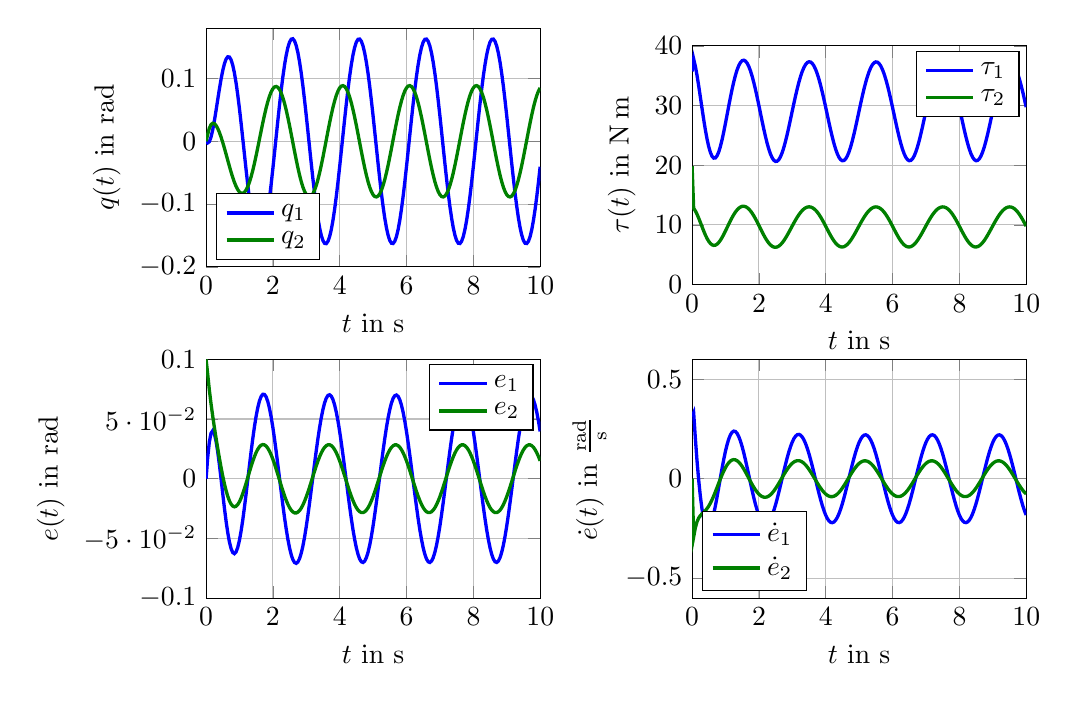
\begin{tikzpicture}

\begin{axis}[%
width=0.35\textwidth,
height=0.25\textwidth,
scale only axis,
xmin=0,
xmax=10,
xlabel={$t$ in $\mathrm{s}$},
xmajorgrids,
ymin=-0.2,
ymax=0.18,
ylabel={$q(t)$ in $\mathrm{rad}$},
ymajorgrids,
name=plot1,
legend style={at={(0.03,0.03)},anchor=south west,draw=black,fill=white,legend cell align=left}
]
\addplot [
color=blue,
solid,
line width=1.2pt
]
table[row sep=crcr]{
0 0\\
0.0468374379716776 -0.00260775825617093\\
0.0968374379716776 -0.000701580971386904\\
0.146837437971678 0.00647829086272891\\
0.196837437971678 0.017841725196221\\
0.246837437971678 0.0322609343439869\\
0.296837437971678 0.0486048125162246\\
0.346837437971678 0.0657688571325622\\
0.396837437971678 0.0827051054192895\\
0.446837437971678 0.0984501350572239\\
0.496837437971678 0.112149722042267\\
0.546837437971678 0.12307922079046\\
0.596837437971678 0.130659112149736\\
0.646837437971678 0.134465461007288\\
0.696837437971678 0.134235246301875\\
0.746837437971678 0.129866686775573\\
0.796837437971678 0.121414803852635\\
0.846837437971678 0.109082557746652\\
0.896837437971678 0.0932079805041726\\
0.946837437971678 0.0742478197938567\\
0.996837437971678 0.0527583005780258\\
1.04683743797167 0.0293737004147362\\
1.09683743797167 0.00478350417354535\\
1.14683743797166 -0.0202910597836074\\
1.19683743797166 -0.0451203089119427\\
1.24683743797165 -0.0689884864488954\\
1.29683743797165 -0.0912145993071283\\
1.34683743797164 -0.111171213593224\\
1.39683743797163 -0.128300851453371\\
1.44683743797163 -0.142129768898969\\
1.49683743797162 -0.152279005895585\\
1.54683743797162 -0.158472677644046\\
1.59683743797161 -0.160543518203298\\
1.64683743797161 -0.158435700977288\\
1.6968374379716 -0.15220495782402\\
1.7468374379716 -0.142016015368488\\
1.79683743797159 -0.128137378516121\\
1.84683743797159 -0.110933527862513\\
1.89683743797158 -0.0908546633829927\\
1.94683743797157 -0.0684242170643191\\
1.99683743797157 -0.0442244603038098\\
2.04683743797156 -0.0188806315361628\\
2.09683743797156 0.00695591163669206\\
2.14683743797155 0.0326249676218908\\
2.19683743797155 0.0574746436830291\\
2.24683743797154 0.0808778772569143\\
2.29683743797154 0.102247890435291\\
2.34683743797153 0.121052235587569\\
2.39683743797152 0.136825186326659\\
2.44683743797152 0.149178312006452\\
2.49683743797151 0.157809134841612\\
2.54683743797151 0.162507802034031\\
2.5968374379715 0.163161713353426\\
2.6468374379715 0.159758035912935\\
2.69683743797149 0.15238402494645\\
2.74683743797149 0.141225066056477\\
2.79683743797148 0.126560372667648\\
2.84683743797147 0.108756319664885\\
2.89683743797147 0.0882574712038145\\
2.94683743797146 0.0655754610604634\\
2.99683743797146 0.041275995077393\\
3.04683743797145 0.0159643510480811\\
3.09683743797145 -0.00973016462512999\\
3.14683743797144 -0.035170294888174\\
3.19683743797144 -0.059726928051629\\
3.24683743797143 -0.082794727646942\\
3.29683743797143 -0.103806876258464\\
3.34683743797142 -0.122248596436017\\
3.39683743797141 -0.137669197921175\\
3.44683743797141 -0.149692475549298\\
3.4968374379714 -0.158025336303728\\
3.5468374379714 -0.162464563048365\\
3.59683743797139 -0.162901628888014\\
3.64683743797139 -0.159325468045502\\
3.69683743797138 -0.151823098555395\\
3.74683743797138 -0.140577992069456\\
3.79683743797137 -0.125866107970996\\
3.84683743797136 -0.108049559638789\\
3.89683743797136 -0.0875679605526183\\
3.94683743797135 -0.0649276005099472\\
3.99683743797135 -0.0406887150703147\\
4.04683743797136 -0.0154512184638729\\
4.09683743797138 0.0101606445502788\\
4.1468374379714 0.0355142217518823\\
4.19683743797141 0.0599844358363405\\
4.24683743797143 0.082969341123552\\
4.29683743797145 0.103904832264513\\
4.34683743797146 0.122278164030311\\
4.39683743797148 0.137640026182765\\
4.4468374379715 0.14961499180149\\
4.49683743797151 0.1579102113137\\
4.54683743797153 0.162322253761186\\
4.59683743797155 0.162742003886161\\
4.64683743797156 0.159157516430551\\
4.69683743797158 0.151654719428851\\
4.7468374379716 0.14041585921445\\
4.79683743797161 0.125715602581188\\
4.84683743797163 0.107914762832282\\
4.89683743797165 0.087451696772249\\
4.94683743797166 0.0648315226049221\\
4.99683743797168 0.0406134217878283\\
5.0468374379717 0.0153963952160302\\
5.09683743797171 -0.0101960704371703\\
5.14683743797173 -0.0355319195327062\\
5.19683743797175 -0.059986511011443\\
5.24683743797176 -0.0829581826669378\\
5.29683743797178 -0.103882972597588\\
5.3468374379718 -0.122248155595739\\
5.39683743797181 -0.137604337120992\\
5.44683743797183 -0.149575921947213\\
5.49683743797185 -0.157869828591123\\
5.54683743797186 -0.162282350122282\\
5.59683743797188 -0.162704069233432\\
5.6468374379719 -0.159122728494122\\
5.69683743797191 -0.151623947302584\\
5.74683743797193 -0.140389678157269\\
5.79683743797195 -0.125694317712416\\
5.84683743797196 -0.107898439451317\\
5.89683743797198 -0.0874401951803917\\
5.946837437972 -0.0648245354799834\\
5.99683743797201 -0.0406105123514408\\
6.04683743797203 -0.0153970346385861\\
6.09683743797205 0.010192467725213\\
6.14683743797206 0.0355259637097945\\
6.19683743797208 0.0599788087376211\\
6.2468374379721 0.0829493135097145\\
6.29683743797211 0.103873470288248\\
6.34683743797213 0.122238494138171\\
6.39683743797215 0.137594921551708\\
6.44683743797216 0.149567083365425\\
6.49683743797218 0.157861822948265\\
6.5468374379722 0.162275360182301\\
6.59683743797221 0.162698209084248\\
6.64683743797223 0.159118049998662\\
6.69683743797225 0.151620447914285\\
6.74683743797226 0.140387309579407\\
6.79683743797228 0.125692994943799\\
6.8468374379723 0.107898049826131\\
6.89683743797232 0.0874406070733161\\
6.94683743797233 0.0648256064078034\\
6.99683743797235 0.040612096259421\\
7.04683743797237 0.0153989882149842\\
7.09683743797238 -0.0101902798092076\\
7.1468374379724 -0.0355236646846832\\
7.19683743797242 -0.0599765067443001\\
7.24683743797243 -0.0829470996854705\\
7.29683743797245 -0.103871417843412\\
7.34683743797247 -0.122236658305536\\
7.39683743797248 -0.137593340269604\\
7.4468374379725 -0.149565778544588\\
7.49683743797252 -0.1578608021718\\
7.54683743797253 -0.162274618695498\\
7.59683743797255 -0.162697731944728\\
7.64683743797257 -0.159117814274828\\
7.69683743797258 -0.15162042483922\\
7.7468374379726 -0.140387466586336\\
7.79683743797262 -0.125693297526833\\
7.84683743797263 -0.107898463185676\\
7.89683743797265 -0.0874410975191613\\
7.94683743797267 -0.0648261425047492\\
7.99683743797268 -0.0406126497107796\\
8.04683743797266 -0.0153995344886489\\
8.09683743797263 0.0101897610989942\\
8.1468374379726 0.0355231896193295\\
8.19683743797257 0.0599760871399343\\
8.24683743797255 0.0829467432977838\\
8.29683743797252 0.103871128704194\\
8.34683743797249 0.122236437155982\\
8.39683743797246 0.137593185056515\\
8.44683743797244 0.149565684948277\\
8.49683743797241 0.157860764138427\\
8.54683743797238 0.162274628951265\\
8.59683743797235 0.162697782474322\\
8.64683743797232 0.159117896751332\\
8.6968374379723 0.15162053099709\\
8.74683743797227 0.140387588532798\\
8.79683743797224 0.125693427990118\\
8.84683743797221 0.10789859570096\\
8.89683743797219 0.0874412265549801\\
8.94683743797216 0.0648262635341656\\
8.99683743797213 0.0406127592327782\\
9.0468374379721 0.01539963000617\\
9.09683743797208 -0.0101896811372592\\
9.14683743797205 -0.0355231259058064\\
9.19683743797202 -0.0599760396159712\\
9.24683743797199 -0.0829467112748184\\
9.29683743797196 -0.103871110991187\\
9.34683743797194 -0.122236432186789\\
9.39683743797191 -0.137593191011843\\
9.44683743797188 -0.149565699868019\\
9.49683743797185 -0.157860786021314\\
9.54683743797183 -0.162274655839904\\
9.5968374379718 -0.162697812524694\\
9.64683743797177 -0.15911792828664\\
9.69683743797174 -0.151620562546534\\
9.74683743797172 -0.140387618856291\\
9.79683743797169 -0.125693456090313\\
9.84683743797166 -0.107898620824143\\
9.89683743797163 -0.0874412481825042\\
9.9468374379716 -0.0648262813661561\\
9.99683743797158 -0.04061277316585\\
};
\addlegendentry{$q_1$};

\addplot [
color=green!50!black,
solid,
line width=1.2pt
]
table[row sep=crcr]{
0 0\\
0.0468374379716776 0.0109242774741655\\
0.0968374379716776 0.0208185851165089\\
0.146837437971678 0.0264628065423215\\
0.196837437971678 0.0286853937364457\\
0.246837437971678 0.028132497902037\\
0.296837437971678 0.0253068983540846\\
0.346837437971678 0.0206116224347446\\
0.396837437971678 0.0143835756817986\\
0.446837437971678 0.00691896594446152\\
0.496837437971678 -0.00150807532556403\\
0.546837437971678 -0.0106325944813896\\
0.596837437971678 -0.0201907801538134\\
0.646837437971678 -0.0299160643176383\\
0.696837437971678 -0.0395386969165397\\
0.746837437971678 -0.0487881462582992\\
0.796837437971678 -0.0573976688079763\\
0.846837437971678 -0.0651103836696214\\
0.896837437971678 -0.0716861987494468\\
0.946837437971678 -0.0769089792529262\\
0.996837437971678 -0.0805934268589172\\
1.04683743797167 -0.0825912422336135\\
1.09683743797167 -0.0827962603259977\\
1.14683743797166 -0.0811483604997177\\
1.19683743797166 -0.0776360476028821\\
1.24683743797165 -0.0722976670832667\\
1.29683743797165 -0.0652212564056382\\
1.34683743797164 -0.0565430525791538\\
1.39683743797163 -0.0464446823817132\\
1.44683743797163 -0.0351490697570692\\
1.49683743797162 -0.0229151133904938\\
1.54683743797162 -0.0100312214303948\\
1.59683743797161 0.00319216111755613\\
1.64683743797161 0.0164308394791633\\
1.6968374379716 0.0293557208624334\\
1.7468374379716 0.041641934479741\\
1.79683743797159 0.0529778960265354\\
1.84683743797159 0.0630739900912066\\
1.89683743797158 0.0716705672547238\\
1.94683743797157 0.0785449986626371\\
1.99683743797157 0.0835175924813599\\
2.04683743797156 0.0864562443357125\\
2.09683743797156 0.0872797576240777\\
2.14683743797155 0.0859598213467302\\
2.19683743797155 0.0825216681217481\\
2.24683743797154 0.0770434531889555\\
2.29683743797154 0.0696544003872555\\
2.34683743797153 0.0605317601810582\\
2.39683743797152 0.0498966255479575\\
2.44683743797152 0.0380086604831652\\
2.49683743797151 0.0251598167994262\\
2.54683743797151 0.0116671480089191\\
2.5968374379715 -0.00213512886931943\\
2.6468374379715 -0.0159041275344789\\
2.69683743797149 -0.0292971053622227\\
2.74683743797149 -0.0419803274285703\\
2.79683743797148 -0.0536376999908953\\
2.84683743797147 -0.0639788974408025\\
2.89683743797147 -0.0727467320599689\\
2.94683743797146 -0.0797235579056005\\
2.99683743797146 -0.0847365530940331\\
3.04683743797145 -0.0876617811939805\\
3.09683743797145 -0.0884269847056713\\
3.14683743797144 -0.0870131054330069\\
3.19683743797144 -0.0834545545336803\\
3.24683743797143 -0.077838269318393\\
3.29683743797143 -0.0703015980292626\\
3.34683743797142 -0.0610290537560153\\
3.39683743797141 -0.0502479809268276\\
3.44683743797141 -0.0382231879579295\\
3.4968374379714 -0.0252506207563628\\
3.5468374379714 -0.0116501838410308\\
3.59683743797139 0.00224214412472932\\
3.64683743797139 0.0160827108868844\\
3.69683743797138 0.0295288787932236\\
3.74683743797138 0.0422477433837342\\
3.79683743797137 0.0539246116849303\\
3.84683743797136 0.0642709744562234\\
3.89683743797136 0.0730317302704901\\
3.94683743797135 0.0799914589721296\\
3.99683743797135 0.0849795924423547\\
4.04683743797136 0.0878743846814065\\
4.09683743797138 0.0886056336254899\\
4.1468374379714 0.0871561477619379\\
4.19683743797141 0.0835619780748741\\
4.24683743797143 0.0779114501760574\\
4.29683743797145 0.0703430360013499\\
4.34683743797146 0.0610421048444811\\
4.39683743797148 0.0502365961411796\\
4.4468374379715 0.0381916667114344\\
4.49683743797151 0.025203386187049\\
4.54683743797153 0.0115915861519177\\
4.59683743797155 -0.00230799179026861\\
4.64683743797156 -0.016152061386998\\
4.69683743797158 -0.0295984441071619\\
4.7468374379716 -0.0423147532139961\\
4.79683743797161 -0.0539868405230124\\
4.84683743797163 -0.0643267413414753\\
4.89683743797165 -0.0730798762074702\\
4.94683743797166 -0.0800313071944905\\
4.99683743797168 -0.0850108964947205\\
5.0468374379717 -0.0878972687602445\\
5.09683743797171 -0.0886205289215942\\
5.14683743797173 -0.0871637278170287\\
5.19683743797175 -0.0835630955054921\\
5.24683743797176 -0.0779070765853039\\
5.29683743797178 -0.0703342065017359\\
5.3468374379718 -0.0610298683247758\\
5.39683743797181 -0.0502219721781524\\
5.44683743797183 -0.0381756098037518\\
5.49683743797185 -0.0251867577371274\\
5.54683743797186 -0.0115751343286409\\
5.59683743797188 0.00232364449937511\\
5.6468374379719 0.0161664234532145\\
5.69683743797191 0.0296111538811837\\
5.74683743797193 0.0423255725298194\\
5.79683743797195 0.0539956441596645\\
5.84683743797196 0.0643335035505262\\
5.89683743797198 0.0730846554536593\\
5.946837437972 0.080034230122522\\
5.99683743797201 0.085012141955558\\
6.04683743797203 0.0878970525350707\\
6.09683743797205 0.0886190895970359\\
6.14683743797206 0.0871613141093053\\
6.19683743797208 0.0835599552119723\\
6.2468374379721 0.0779034472583865\\
6.29683743797211 0.070330307883979\\
6.34683743797213 0.0610258965445021\\
6.39683743797215 0.0502180956704806\\
6.44683743797216 0.0381719668855211\\
6.49683743797218 0.0251834557226176\\
6.5468374379722 0.0115722500281057\\
6.59683743797221 -0.00232606309940909\\
6.64683743797223 -0.0161683545637066\\
6.69683743797225 -0.0296125985949137\\
6.74683743797226 -0.0423265510759152\\
6.79683743797228 -0.0539961919729733\\
6.8468374379723 -0.0643336673699655\\
6.89683743797232 -0.0730844896224091\\
6.94683743797233 -0.0800337932167913\\
6.99683743797235 -0.0850114938234833\\
7.04683743797237 -0.0878962517877544\\
7.09683743797238 -0.0886181915626736\\
7.1468374379724 -0.087160369239617\\
7.19683743797242 -0.0835590079168255\\
7.24683743797243 -0.077902535137414\\
7.29683743797245 -0.0703294613205654\\
7.34683743797247 -0.061025138625366\\
7.39683743797248 -0.0502174423916232\\
7.4468374379725 -0.0381714276019464\\
7.49683743797252 -0.0251830337952805\\
7.54683743797253 -0.0115719436179698\\
7.59683743797255 0.00232626014236492\\
7.64683743797257 0.0161684517682181\\
7.69683743797258 0.0296126079410979\\
7.7468374379726 0.0423264861146687\\
7.79683743797262 0.0539960670252182\\
7.84683743797263 0.0643334968289305\\
7.89683743797265 0.0730842873721096\\
7.94683743797267 0.0800335721708141\\
7.99683743797268 0.0850112655808692\\
8.04683743797266 0.0878960263975887\\
8.09683743797263 0.08861797738593\\
8.1468374379726 0.0871601728955237\\
8.19683743797257 0.0835588343010021\\
8.24683743797255 0.0779023874996649\\
8.29683743797252 0.0703293413910259\\
8.34683743797249 0.0610250467783547\\
8.39683743797246 0.0502173778369488\\
8.44683743797244 0.0381713885936146\\
8.49683743797241 0.0251830178477446\\
8.54683743797238 0.0115719477204741\\
8.59683743797235 -0.00232623932199901\\
8.64683743797232 -0.0161684176977583\\
8.6968374379723 -0.0296125640617331\\
8.74683743797227 -0.0423264357062625\\
8.79683743797224 -0.0539960131007044\\
8.84683743797221 -0.0643334420576733\\
8.89683743797219 -0.0730842340304734\\
8.94683743797216 -0.0800335221170475\\
8.99683743797213 -0.0850112202507424\\
9.0468374379721 -0.0878959868169933\\
9.09683743797208 -0.0886179441967657\\
9.14683743797205 -0.0871601463915294\\
9.19683743797202 -0.0835588144706018\\
9.24683743797199 -0.0779023740733225\\
9.29683743797196 -0.0703293338909437\\
9.34683743797194 -0.0610250445686146\\
9.39683743797191 -0.050217380172384\\
9.44683743797188 -0.0381713946658699\\
9.49683743797185 -0.0251830268271644\\
9.54683743797183 -0.0115719587926938\\
9.5968374379718 0.00232622692558808\\
9.64683743797177 0.0161684046761484\\
9.69683743797174 0.0296125510271475\\
9.74683743797172 0.0423264231734534\\
9.79683743797169 0.0539960014821322\\
9.84683743797166 0.0643334316637684\\
9.89683743797163 0.0730842250740457\\
9.9468374379716 0.0800335147208725\\
9.99683743797158 0.0850112144573927\\
};
\addlegendentry{$q_2$};

\end{axis}

\begin{axis}[%
width=0.35\textwidth,
height=0.25\textwidth,
scale only axis,
xmin=0,
xmax=10,
xlabel={$t$ in $\mathrm{s}$},
xmajorgrids,
ymin=-0.1,
ymax=0.1,
ylabel={$e(t)$ in $\mathrm{rad}$},
ymajorgrids,
name=plot3,
at=(plot1.below south west),
anchor=above north west,
legend style={draw=black,fill=white,legend cell align=left}
]
\addplot [
color=blue,
solid,
line width=1.2pt
]
table[row sep=crcr]{
0 0\\
0.0468374379716776 0.0172691328625021\\
0.0968374379716776 0.0306568503003278\\
0.146837437971678 0.038033275042104\\
0.196837437971678 0.0401301148065092\\
0.246837437971678 0.037743720658267\\
0.296837437971678 0.0317089105472677\\
0.346837437971678 0.0228763435843802\\
0.396837437971678 0.0120888339128977\\
0.446837437971678 0.000158401500802013\\
0.496837437971678 -0.012154657691431\\
0.546837437971678 -0.0241598389957233\\
0.596837437971678 -0.0352511363854921\\
0.646837437971678 -0.0449181522777691\\
0.696837437971678 -0.0527535565384822\\
0.746837437971678 -0.058456965602504\\
0.796837437971678 -0.0618353956004485\\
0.846837437971678 -0.0628005051792365\\
0.896837437971678 -0.0613629013570642\\
0.946837437971678 -0.0576238456034152\\
0.996837437971678 -0.0517647687606271\\
1.04683743797167 -0.044035075021066\\
1.09683743797167 -0.0347387735024833\\
1.14683743797166 -0.0242205061212212\\
1.19683743797166 -0.0128515310907821\\
1.24683743797165 -0.00101616855335254\\
1.29683743797165 0.010900876243642\\
1.34683743797164 0.0225260128762873\\
1.39683743797163 0.0335069121211878\\
1.44683743797163 0.0435212323409461\\
1.49683743797162 0.0522839415447497\\
1.54683743797162 0.0595532958493064\\
1.59683743797161 0.065135542439048\\
1.64683743797161 0.0688883922477592\\
1.6968374379716 0.0707232680606132\\
1.7468374379716 0.0706062941954015\\
1.79683743797159 0.0685579702639128\\
1.84683743797159 0.0646514752950722\\
1.89683743797158 0.0590095842358548\\
1.94683743797157 0.0518002428738453\\
1.99683743797157 0.0432309284863765\\
2.04683743797156 0.0335420061424584\\
2.09683743797156 0.0229993576922128\\
2.14683743797155 0.0118865982829068\\
2.19683743797155 0.000497196319667451\\
2.24683743797154 -0.0108732222546911\\
2.29683743797154 -0.0219341673718255\\
2.34683743797153 -0.0324070348706476\\
2.39683743797152 -0.042031246994487\\
2.44683743797152 -0.0505697754484341\\
2.49683743797151 -0.0578140704907762\\
2.54683743797151 -0.0635884202392872\\
2.5968374379715 -0.0677537375891649\\
2.6468374379715 -0.0702107271833907\\
2.69683743797149 -0.0709023351830228\\
2.74683743797149 -0.0698153448833665\\
2.79683743797148 -0.066980964415412\\
2.84683743797147 -0.0624742670974133\\
2.89683743797147 -0.0564123920566438\\
2.94683743797146 -0.0489514868699554\\
2.99683743797146 -0.0402824632599251\\
3.04683743797145 -0.0306257256543425\\
3.09683743797145 -0.0202251047037418\\
3.14683743797144 -0.00934127101659258\\
3.19683743797144 0.00175508804896059\\
3.24683743797143 0.0127900726447435\\
3.29683743797143 0.0234931531950194\\
3.34683743797142 0.0336033957191123\\
3.39683743797141 0.042875258589014\\
3.44683743797141 0.0510839389912861\\
3.4968374379714 0.0580302719528934\\
3.5468374379714 0.0635451812536152\\
3.59683743797139 0.0674936531237432\\
3.64683743797139 0.0697781593159428\\
3.69683743797138 0.0703414087919483\\
3.74683743797138 0.0691682708963205\\
3.79683743797137 0.0662866997187322\\
3.84683743797136 0.0617675070712863\\
3.89683743797136 0.0557228814054149\\
3.94683743797135 0.0483036263194051\\
3.99683743797135 0.0396951832528122\\
4.04683743797136 0.0301125930701064\\
4.09683743797138 0.0197946247785728\\
4.1468374379714 0.00899734415287149\\
4.19683743797141 -0.00201259583367808\\
4.24683743797143 -0.0129646861213537\\
4.29683743797145 -0.0235911092010644\\
4.34683743797146 -0.0336329633134003\\
4.39683743797148 -0.0428460868505973\\
4.4468374379715 -0.0510064552434732\\
4.49683743797151 -0.0579151469628648\\
4.54683743797153 -0.0634028719664427\\
4.59683743797155 -0.067334028121904\\
4.64683743797156 -0.0696102077010169\\
4.69683743797158 -0.07017302966544\\
4.7468374379716 -0.0690061380413637\\
4.79683743797161 -0.0661361943289861\\
4.84683743797163 -0.0616327102648529\\
4.89683743797165 -0.0556066176251312\\
4.94683743797166 -0.0482075484144761\\
4.99683743797168 -0.0396198899704302\\
5.0468374379717 -0.0300577698223675\\
5.09683743797171 -0.0197591988917813\\
5.14683743797173 -0.00897964637214161\\
5.19683743797175 0.00201467100869511\\
5.24683743797176 0.0129535276646645\\
5.29683743797178 0.0235692495340762\\
5.3468374379718 0.0336029548787794\\
5.39683743797181 0.0428103977887914\\
5.44683743797183 0.0509673853891794\\
5.49683743797185 0.057874764240287\\
5.54683743797186 0.0633629683275543\\
5.59683743797188 0.0672960934692068\\
5.6468374379719 0.0695754197646338\\
5.69683743797191 0.0701422575392339\\
5.74683743797193 0.0689799569842564\\
5.79683743797195 0.0661149094602976\\
5.84683743797196 0.0616163868839812\\
5.89683743797198 0.0555951160333735\\
5.946837437972 0.0482005612896408\\
5.99683743797201 0.0396169805341477\\
6.04683743797203 0.030058409245027\\
6.09683743797205 0.0197628016038389\\
6.14683743797206 0.00898560219514719\\
6.19683743797208 -0.00200696873478755\\
6.2468374379721 -0.0129446585073665\\
6.29683743797211 -0.0235597472246741\\
6.34683743797213 -0.033593293421163\\
6.39683743797215 -0.0428009822194734\\
6.44683743797216 -0.0509585468073733\\
6.49683743797218 -0.0578667585974277\\
6.5468374379722 -0.0633559783875882\\
6.59683743797221 -0.0672902333200542\\
6.64683743797223 -0.0695707412692204\\
6.69683743797225 -0.0701387581509958\\
6.74683743797226 -0.0689775884064674\\
6.79683743797228 -0.0661135866917656\\
6.8468374379723 -0.0616159972588879\\
6.89683743797232 -0.0555955279263972\\
6.94683743797233 -0.048201632217564\\
6.99683743797235 -0.0396185644422327\\
7.04683743797237 -0.0300603628215288\\
7.09683743797238 -0.0197649895199443\\
7.1468374379724 -0.00898790122035235\\
7.19683743797242 0.00200466674138114\\
7.24683743797243 0.0129424446830476\\
7.29683743797245 0.0235576947797752\\
7.34683743797247 0.0335914575884795\\
7.39683743797248 0.0427994009373359\\
7.4468374379725 0.0509572419865192\\
7.49683743797252 0.0578657378209613\\
7.54683743797253 0.0633552369008008\\
7.59683743797255 0.0672897561805662\\
7.64683743797257 0.0695705055454333\\
7.69683743797258 0.0701387350759917\\
7.7468374379726 0.0689777454134701\\
7.79683743797262 0.0661138892748834\\
7.84683743797263 0.0616164106185262\\
7.89683743797265 0.0555960183723418\\
7.94683743797267 0.0482021683146136\\
7.99683743797268 0.0396191178936961\\
8.04683743797266 0.0300609090952846\\
8.09683743797263 0.0197655082302319\\
8.1468374379726 0.00898837628576325\\
8.19683743797257 -0.00200424713697459\\
8.24683743797255 -0.012942088295335\\
8.29683743797252 -0.023557405640544\\
8.34683743797249 -0.0335912364389215\\
8.39683743797246 -0.042799245724249\\
8.44683743797244 -0.0509571483902114\\
8.49683743797241 -0.0578656997875883\\
8.54683743797238 -0.0633552471565606\\
8.59683743797235 -0.0672898067101418\\
8.64683743797232 -0.0695705880219036\\
8.6968374379723 -0.0701388412338097\\
8.74683743797227 -0.068977867359859\\
8.79683743797224 -0.066114019738074\\
8.84683743797221 -0.061616543133694\\
8.89683743797219 -0.0555961474080229\\
8.94683743797216 -0.0482022893438726\\
8.99683743797213 -0.0396192274155213\\
9.0468374379721 -0.0300610046126334\\
9.09683743797208 -0.0197655881918008\\
9.14683743797205 -0.00898843999913048\\
9.19683743797202 0.00200419961315364\\
9.24683743797199 0.0129420562724939\\
9.29683743797196 0.0235573879276415\\
9.34683743797194 0.0335912314698094\\
9.39683743797191 0.0427992516796331\\
9.44683743797188 0.0509571633099829\\
9.49683743797185 0.0578657216704774\\
9.54683743797183 0.0633552740451748\\
9.5968374379718 0.0672898367604611\\
9.64683743797177 0.069570619557134\\
9.69683743797174 0.0701388727831526\\
9.74683743797172 0.0689778976832302\\
9.79683743797169 0.0661140478381295\\
9.84683743797166 0.061616568256723\\
9.89683743797163 0.0555961690353819\\
9.9468374379716 0.0482023071756915\\
9.99683743797158 0.039619241348419\\
};
\addlegendentry{$e_1$};

\addplot [
color=green!50!black,
solid,
line width=1.2pt
]
table[row sep=crcr]{
0 0.1\\
0.0468374379716776 0.0879951043205709\\
0.0968374379716776 0.0745893906477353\\
0.146837437971678 0.0630845021871971\\
0.196837437971678 0.0527962960269475\\
0.246837437971678 0.0432772232710317\\
0.296837437971678 0.0342725098981016\\
0.346837437971678 0.0256704301326707\\
0.396837437971678 0.01746150346531\\
0.446837437971678 0.00970500824598014\\
0.496837437971678 0.0025016071429629\\
0.546837437971678 -0.00402878012494168\\
0.596837437971678 -0.0097644891751276\\
0.646837437971678 -0.0145955015871947\\
0.696837437971678 -0.0184331430861906\\
0.746837437971678 -0.0212165087439547\\
0.796837437971678 -0.0229160542555161\\
0.846837437971678 -0.0235348170473211\\
0.896837437971678 -0.0231077405827404\\
0.946837437971678 -0.0216995573050997\\
0.996837437971678 -0.0194016374919187\\
1.04683743797167 -0.0163281395611231\\
1.09683743797167 -0.0126117154382474\\
1.14683743797166 -0.008398948229803\\
1.19683743797166 -0.00384564216051488\\
1.24683743797165 0.000887945910192159\\
1.29683743797165 0.00564184815344396\\
1.34683743797164 0.010261000011728\\
1.39683743797163 0.0145996032345917\\
1.44683743797163 0.0185250955666125\\
1.49683743797162 0.0219215815730779\\
1.54683743797162 0.0246925960367075\\
1.59683743797161 0.0267631082113653\\
1.64683743797161 0.0280807264256498\\
1.6968374379716 0.0286161191402773\\
1.7468374379716 0.0283627205224945\\
1.79683743797159 0.0273358270369406\\
1.84683743797159 0.0255712106257224\\
1.89683743797158 0.0231233720774535\\
1.94683743797157 0.0200635378953834\\
1.99683743797157 0.0164774718694757\\
2.04683743797156 0.0124631374590292\\
2.09683743797156 0.00812821814017781\\
2.14683743797155 0.00358748738280593\\
2.19683743797155 -0.001039978358331\\
2.24683743797154 -0.00563373201585679\\
2.29683743797154 -0.0100749921350334\\
2.34683743797153 -0.0142497076136017\\
2.39683743797152 -0.0180515464008032\\
2.44683743797152 -0.0213846862926743\\
2.49683743797151 -0.0241662849819756\\
2.54683743797151 -0.0263285226151975\\
2.5968374379715 -0.027820140459569\\
2.6468374379715 -0.0286074383703033\\
2.69683743797149 -0.0286747346404598\\
2.74683743797149 -0.0280243275736405\\
2.79683743797148 -0.02667602307256\\
2.84683743797147 -0.0246663032761104\\
2.89683743797147 -0.0220472072721975\\
2.94683743797146 -0.0188849786524142\\
2.99683743797146 -0.0152585112568021\\
3.04683743797145 -0.0112576006007663\\
3.09683743797145 -0.00698099105859459\\
3.14683743797144 -0.00253420329654463\\
3.19683743797144 0.00197286477024319\\
3.24683743797143 0.00642854814527008\\
3.29683743797143 0.0107221897770127\\
3.34683743797142 0.0147470011885281\\
3.39683743797141 0.0184029017796405\\
3.44683743797141 0.0215992137674045\\
3.4968374379714 0.0242570889388775\\
3.5468374379714 0.026311558447275\\
3.59683743797139 0.027713125204126\\
3.64683743797139 0.0284288550178667\\
3.69683743797138 0.0284429612094308\\
3.74683743797138 0.0277569116184519\\
3.79683743797137 0.0263891113785044\\
3.84683743797136 0.0243742262606735\\
3.89683743797136 0.0217622090616653\\
3.94683743797135 0.0186170775858793\\
3.99683743797135 0.0150154719084802\\
4.04683743797136 0.0110449971133443\\
4.09683743797138 0.00680234213878234\\
4.1468374379714 0.00239116096762002\\
4.19683743797141 -0.0020802883114327\\
4.24683743797143 -0.00650172900293421\\
4.29683743797145 -0.0107636277491054\\
4.34683743797146 -0.014760052277006\\
4.39683743797148 -0.0183915169940121\\
4.4468374379715 -0.0215676925209366\\
4.49683743797151 -0.0242098543695984\\
4.54683743797153 -0.026252960758203\\
4.59683743797155 -0.027647277538633\\
4.64683743797156 -0.0283595045178028\\
4.69683743797158 -0.0283733958955433\\
4.7468374379716 -0.0276899017882396\\
4.79683743797161 -0.0263268825404678\\
4.84683743797163 -0.0243184593754601\\
4.89683743797165 -0.0217140631247139\\
4.94683743797166 -0.0185772293635347\\
4.99683743797168 -0.0149841678561154\\
5.0468374379717 -0.011022113034491\\
5.09683743797171 -0.00678744684264666\\
5.14683743797173 -0.00238358091248247\\
5.19683743797175 0.00208140574211151\\
5.24683743797176 0.00649735541225416\\
5.29683743797178 0.0107547982495756\\
5.3468374379718 0.0147478157573937\\
5.39683743797181 0.0183768930310842\\
5.44683743797183 0.0215516356133575\\
5.49683743797185 0.0241932259197816\\
5.54683743797186 0.02623650893503\\
5.59683743797188 0.0276316248296265\\
5.6468374379719 0.0283451424516803\\
5.69683743797191 0.0283606861216069\\
5.74683743797193 0.0276790824724913\\
5.79683743797195 0.0263180789038784\\
5.84683743797196 0.0243116971664579\\
5.89683743797198 0.0217092838785583\\
5.946837437972 0.0185743064355206\\
5.99683743797201 0.0149829223952789\\
6.04683743797203 0.0110223292596494\\
6.09683743797205 0.00678888616717342\\
6.14683743797206 0.00238599462015923\\
6.19683743797208 -0.00207826544865265\\
6.2468374379721 -0.00649372608541013\\
6.29683743797211 -0.0107508996319031\\
6.34683743797213 -0.014743843977213\\
6.39683743797215 -0.018373016523512\\
6.44683743797216 -0.0215479926952301\\
6.49683743797218 -0.0241899239053769\\
6.5468374379722 -0.0262336246345985\\
6.59683743797221 -0.0276292062296928\\
6.64683743797223 -0.028343211341282\\
6.69683743797225 -0.0283592414079626\\
6.74683743797226 -0.0276781039264703\\
6.79683743797228 -0.026317531090632\\
6.8468374379723 -0.024311533347067\\
6.89683743797232 -0.0217094497098419\\
6.94683743797233 -0.0185747433412687\\
6.99683743797235 -0.0149835705273547\\
7.04683743797237 -0.0110231300069503\\
7.09683743797238 -0.00678978420150439\\
7.1468374379724 -0.00238693948980089\\
7.19683743797242 0.00207731815356661\\
7.24683743797243 0.00649281396451103\\
7.29683743797245 0.0107500530685737\\
7.34683743797247 0.0147430860581701\\
7.39683743797248 0.018372363244754\\
7.4468374379725 0.0215474534117591\\
7.49683743797252 0.0241895019781446\\
7.54683743797253 0.0262333182245666\\
7.59683743797255 0.027629009186837\\
7.64683743797257 0.0283431141368646\\
7.69683743797258 0.0283592320618637\\
7.7468374379726 0.0276781688877919\\
7.79683743797262 0.0263176560384495\\
7.84683743797263 0.0243117038881507\\
7.89683743797265 0.0217096519601747\\
7.94683743797267 0.0185749643872634\\
7.99683743797268 0.0149837987699698\\
8.04683743797266 0.0110233553971025\\
8.09683743797263 0.00678999837822467\\
8.1468374379726 0.00238713583386575\\
8.19683743797257 -0.0020771445377722\\
8.24683743797255 -0.0064926663267873\\
8.29683743797252 -0.0107499331390518\\
8.34683743797249 -0.0147429942111657\\
8.39683743797246 -0.0183722986900742\\
8.44683743797244 -0.0215474144034077\\
8.49683743797241 -0.0241894860305749\\
8.54683743797238 -0.0262333223270234\\
8.59683743797235 -0.0276290300071442\\
8.64683743797232 -0.0283431482072566\\
8.6968374379723 -0.0283592759411555\\
8.74683743797227 -0.0276782192961239\\
8.79683743797224 -0.0263177099628932\\
8.84683743797221 -0.024311758659347\\
8.89683743797219 -0.0217097053017646\\
8.94683743797216 -0.0185750144410035\\
8.99683743797213 -0.0149838441000949\\
9.0468374379721 -0.0110233949777235\\
9.09683743797208 -0.00679003156744112\\
9.14683743797205 -0.00238716233793757\\
9.19683743797202 0.00207712470727084\\
9.24683743797199 0.00649265290032297\\
9.29683743797196 0.0107499256388299\\
9.34683743797194 0.0147429920012713\\
9.39683743797191 0.018372301025344\\
9.44683743797188 0.0215474204754913\\
9.49683743797185 0.0241894950098206\\
9.54683743797183 0.0262333333990709\\
9.5968374379718 0.0276290424033887\\
9.64683743797177 0.0283431612287107\\
9.69683743797174 0.0283592889755993\\
9.74683743797172 0.0276782318288088\\
9.79683743797169 0.0263177215813617\\
9.84683743797166 0.0243117690531714\\
9.89683743797163 0.0217097142581369\\
9.9468374379716 0.0185750218371495\\
9.99683743797158 0.0149838498934429\\
};
\addlegendentry{$e_2$};

\end{axis}

\begin{axis}[%
width=0.35\textwidth,
height=0.25\textwidth,
scale only axis,
xmin=0,
xmax=10,
xlabel={$t$ in $\mathrm{s}$},
xmajorgrids,
ymin=-0.6,
ymax=0.6,
ylabel={$\dot{e}(t)$ in $\mathrm{\frac{rad}{s}}$},
ymajorgrids,
name=plot2,
at=(plot3.right of south east),
anchor=left of south west,
legend style={at={(0.03,0.03)},anchor=south west,draw=black,fill=white,legend cell align=left}
]
\addplot [
color=blue,
solid,
line width=1.2pt
]
table[row sep=crcr]{
0 0.314159265358979\\
0.0468374379716776 0.331732299503059\\
0.0968374379716776 0.205105646809838\\
0.146837437971678 0.0917870989156097\\
0.196837437971678 -0.00611787267578029\\
0.246837437971678 -0.0876275633400841\\
0.296837437971678 -0.152189379706086\\
0.346837437971678 -0.199721038358337\\
0.396837437971678 -0.230612125007389\\
0.446837437971678 -0.245694947057344\\
0.496837437971678 -0.246194441764899\\
0.546837437971678 -0.23366496716779\\
0.596837437971678 -0.209920002554917\\
0.646837437971678 -0.176959156914057\\
0.696837437971678 -0.136895512354726\\
0.746837437971678 -0.0918853069306485\\
0.796837437971678 -0.0440613408621864\\
0.846837437971678 0.00452874615188031\\
0.896837437971678 0.0519781305347336\\
0.946837437971678 0.0965690280354294\\
0.996837437971678 0.136812015279902\\
1.04683743797167 0.171475097930706\\
1.09683743797167 0.199601591742458\\
1.14683743797166 0.22051657927455\\
1.19683743797166 0.233822564080636\\
1.24683743797165 0.239385791876945\\
1.29683743797165 0.237315363805138\\
1.34683743797164 0.227937593047814\\
1.39683743797163 0.211767992892591\\
1.44683743797163 0.189482860808505\\
1.49683743797162 0.161891745554478\\
1.54683743797162 0.129911308787957\\
1.59683743797161 0.0945403888412187\\
1.64683743797161 0.0568355897037824\\
1.6968374379716 0.0178865479313335\\
1.7468374379716 -0.0212098020244055\\
1.79683743797159 -0.0593761902366486\\
1.84683743797159 -0.0955828068738713\\
1.89683743797158 -0.128874906322793\\
1.94683743797157 -0.158398718346197\\
1.99683743797157 -0.1834239684156\\
2.04683743797156 -0.20336145439366\\
2.09683743797156 -0.217774591428283\\
2.14683743797155 -0.226384522446682\\
2.19683743797155 -0.229069147630992\\
2.24683743797154 -0.225857088995963\\
2.29683743797154 -0.216918038438196\\
2.34683743797153 -0.202551059379428\\
2.39683743797152 -0.183172215359158\\
2.44683743797152 -0.159302444792323\\
2.49683743797151 -0.13155600261458\\
2.54683743797151 -0.100629185442165\\
2.5968374379715 -0.0672885827674441\\
2.6468374379715 -0.0323578585268893\\
2.69683743797149 0.00329787889543873\\
2.74683743797149 0.038790719785469\\
2.79683743797148 0.0732316507203675\\
2.84683743797147 0.105754684991624\\
2.89683743797147 0.135542182230437\\
2.94683743797146 0.161849673502514\\
2.99683743797146 0.184028354369739\\
3.04683743797145 0.20154358356658\\
3.09683743797145 0.213988197544465\\
3.14683743797144 0.221090122162832\\
3.19683743797144 0.222714489448671\\
3.24683743797143 0.218861097667236\\
3.29683743797143 0.209658461598434\\
3.34683743797142 0.195355815521596\\
3.39683743797141 0.176314249481305\\
3.44683743797141 0.152997739349706\\
3.4968374379714 0.125964280196534\\
3.5468374379714 0.0958567812379545\\
3.59683743797139 0.0633929565456518\\
3.64683743797139 0.0293532480320399\\
3.69683743797138 -0.0054341020226249\\
3.74683743797138 -0.0401113586616303\\
3.79683743797137 -0.0738129517295838\\
3.84683743797136 -0.10568979833953\\
3.89683743797136 -0.134934996390487\\
3.94683743797135 -0.160809167451103\\
3.99683743797135 -0.182663582414968\\
4.04683743797136 -0.199959382426482\\
4.09683743797138 -0.212281679612153\\
4.1468374379714 -0.219347989850435\\
4.19683743797141 -0.221011172743636\\
4.24683743797143 -0.217257682391868\\
4.29683743797145 -0.208202342618202\\
4.34683743797146 -0.194080980990244\\
4.39683743797148 -0.175242082238456\\
4.4468374379715 -0.152138211593946\\
4.49683743797151 -0.125317417733367\\
4.54683743797153 -0.0954142826319891\\
4.59683743797155 -0.0631398679739587\\
4.64683743797156 -0.0292696135974648\\
4.69683743797158 0.00537167517979573\\
4.7468374379716 0.0399282632316586\\
4.79683743797161 0.0735352991125242\\
4.84683743797163 0.10534331043853\\
4.89683743797165 0.134544079354736\\
4.94683743797166 0.160396170888665\\
4.99683743797168 0.182248243326741\\
5.0468374379717 0.199558449128465\\
5.09683743797171 0.211908706637268\\
5.14683743797173 0.219013290154738\\
5.19683743797175 0.220721908810575\\
5.24683743797176 0.217018073616181\\
5.29683743797178 0.208013963290049\\
5.3468374379718 0.193943121777706\\
5.39683743797181 0.175152148500097\\
5.44683743797183 0.15209213405003\\
5.49683743797185 0.125310054621407\\
5.54683743797186 0.0954397969295498\\
5.59683743797188 0.0631920679921195\\
5.6468374379719 0.0293422496906916\\
5.69683743797191 -0.0052846612753186\\
5.74683743797193 -0.0398325370384516\\
5.79683743797195 -0.0734359786611393\\
5.84683743797196 -0.105244855546167\\
5.89683743797198 -0.134450221682003\\
5.946837437972 -0.160309881140328\\
5.99683743797201 -0.182171731660903\\
6.04683743797203 -0.19949319449704\\
6.09683743797205 -0.211855510374744\\
6.14683743797206 -0.218972348720511\\
6.19683743797208 -0.220692900277863\\
6.2468374379721 -0.217000252397613\\
6.29683743797211 -0.208006257774125\\
6.34683743797213 -0.193944230044274\\
6.39683743797215 -0.175160628050974\\
6.44683743797216 -0.152106482448702\\
6.49683743797218 -0.125328778972385\\
6.5468374379722 -0.0954614711295098\\
6.59683743797221 -0.0632153775558927\\
6.64683743797223 -0.0293660246333085\\
6.69683743797225 0.005261424557122\\
6.74683743797226 0.0398106636819215\\
6.79683743797228 0.0734161117483831\\
6.8468374379723 0.105227459715838\\
6.89683743797232 0.134435592706282\\
6.94683743797233 0.160298160298613\\
6.99683743797235 0.182162923792126\\
7.04683743797237 0.199487188642105\\
7.09683743797238 0.211852101940921\\
7.1468374379724 0.218971262130649\\
7.19683743797242 0.220693811129258\\
7.24683743797243 0.217002808261263\\
7.29683743797245 0.208010096917092\\
7.34683743797247 0.193948997547086\\
7.39683743797248 0.175165989000711\\
7.4468374379725 0.15211213209558\\
7.49683743797252 0.125334449922384\\
7.54683743797253 0.095466937792593\\
7.59683743797255 0.0632204581698197\\
7.64683743797257 0.0293705812366758\\
7.69683743797258 -0.00525748781637578\\
7.7468374379726 -0.0398074035336993\\
7.79683743797262 -0.0734135497496648\\
7.84683743797263 -0.105225586869498\\
7.89683743797265 -0.134434374495833\\
7.94683743797267 -0.160297541916961\\
7.99683743797268 -0.182162835366821\\
8.04683743797266 -0.199487550279153\\
8.09683743797263 -0.211852828428303\\
8.1468374379726 -0.218972267164825\\
8.19683743797257 -0.220695010956052\\
8.24683743797255 -0.217004124656591\\
8.29683743797252 -0.208011459471163\\
8.34683743797249 -0.193950345254618\\
8.39683743797246 -0.175167271195586\\
8.44683743797244 -0.152113308797509\\
8.49683743797241 -0.125335491683418\\
8.54683743797238 -0.0954678251415792\\
8.59683743797235 -0.0632211807540664\\
8.64683743797232 -0.0293711367536774\\
8.6968374379723 0.00525709481544648\\
8.74683743797227 0.0398071629005454\\
8.79683743797224 0.07341344700061\\
8.84683743797221 0.105225604409321\\
8.89683743797219 0.134434492769903\\
8.94683743797216 0.160297740464991\\
8.99683743797213 0.182163093756967\\
9.0468374379721 0.199487848905965\\
9.09683743797208 0.211853149162772\\
9.14683743797205 0.218972593850399\\
9.19683743797202 0.220695329750562\\
9.24683743797199 0.217004424226436\\
9.29683743797196 0.208011731050362\\
9.34683743797194 0.193950582586481\\
9.39683743797191 0.175167470378464\\
9.44683743797188 0.152113468057849\\
9.49683743797185 0.125335611099259\\
9.54683743797183 0.0954679063378974\\
9.5968374379718 0.0632212265884258\\
9.64683743797177 0.029371151007111\\
9.69683743797174 -0.00525710773109458\\
9.74683743797172 -0.0398071982109137\\
9.79683743797169 -0.0734134998075951\\
9.84683743797166 -0.105225669897257\\
9.89683743797163 -0.134434566377524\\
9.9468374379716 -0.160297818022587\\
9.99683743797158 -0.182163171588927\\
};
\addlegendentry{$\dot{e}_1$};

\addplot [
color=green!50!black,
solid,
line width=1.2pt
]
table[row sep=crcr]{
0 -0\\
0.0468374379716776 -0.292759020026348\\
0.0968374379716776 -0.247246408711962\\
0.146837437971678 -0.216815361343858\\
0.196837437971678 -0.197624622507212\\
0.246837437971678 -0.185257849866192\\
0.296837437971678 -0.176391586658059\\
0.346837437971678 -0.16860217065955\\
0.396837437971678 -0.160204436980867\\
0.446837437971678 -0.150118694072148\\
0.496837437971678 -0.137758002612444\\
0.546837437971678 -0.122930084912801\\
0.596837437971678 -0.10575020412446\\
0.646837437971678 -0.0865630493314516\\
0.696837437971678 -0.0658729701348364\\
0.746837437971678 -0.0442827439998151\\
0.796837437971678 -0.0224413981237409\\
0.846837437971678 -0.00100148700605579\\
0.896837437971678 0.0194142300833481\\
0.946837437971678 0.0382373790428039\\
0.996837437971678 0.0549710621174014\\
1.04683743797167 0.0692010379325736\\
1.09683743797167 0.0806026246131485\\
1.14683743797166 0.0889446993567078\\
1.19683743797166 0.0940916867418733\\
1.24683743797165 0.0960038702518476\\
1.29683743797165 0.0947358814031445\\
1.34683743797164 0.0904329391794015\\
1.39683743797163 0.0833243856303921\\
1.44683743797163 0.0737142748074923\\
1.49683743797162 0.061969144214792\\
1.54683743797162 0.0485035193967917\\
1.59683743797161 0.033764059770536\\
1.64683743797161 0.0182134591269267\\
1.6968374379716 0.00231522144946517\\
1.7468374379716 -0.0134797565329242\\
1.79683743797159 -0.0287442061220997\\
1.84683743797159 -0.0430829399360685\\
1.89683743797158 -0.0561389749230583\\
1.94683743797157 -0.0675978744980294\\
1.99683743797157 -0.0771910121800485\\
2.04683743797156 -0.0846984252633384\\
2.09683743797156 -0.0899517218363264\\
2.14683743797155 -0.0928371839813303\\
2.19683743797155 -0.0932988578793661\\
2.24683743797154 -0.0913411278598043\\
2.29683743797154 -0.0870301094188579\\
2.34683743797153 -0.0804932040470697\\
2.39683743797152 -0.0719163315205563\\
2.44683743797152 -0.0615386494597786\\
2.49683743797151 -0.0496449167998497\\
2.54683743797151 -0.0365559820930629\\
2.5968374379715 -0.022618114630154\\
2.6468374379715 -0.00819200418102323\\
2.69683743797149 0.00635778038697726\\
2.74683743797149 0.0206722489033129\\
2.79683743797148 0.0344059985143949\\
2.84683743797147 0.0472337074359945\\
2.89683743797147 0.0588553281096957\\
2.94683743797146 0.0690003958004479\\
2.99683743797146 0.0774319480750813\\
3.04683743797145 0.0839504886619493\\
3.09683743797145 0.088398239170488\\
3.14683743797144 0.0906636491263766\\
3.19683743797144 0.0906858462043382\\
3.24683743797143 0.0884584775058086\\
3.29683743797143 0.084032278778506\\
3.34683743797142 0.0775157420890331\\
3.39683743797141 0.0690734280495375\\
3.44683743797141 0.0589217478120561\\
3.4968374379714 0.0473223628688583\\
3.5468374379714 0.03457365152727\\
3.59683743797139 0.0210009127784259\\
3.64683743797139 0.00694608323868429\\
3.69683743797138 -0.00724228302596996\\
3.74683743797138 -0.0212181684424924\\
3.79683743797137 -0.0346460119454284\\
3.84683743797136 -0.0472073048126767\\
3.89683743797136 -0.058606035057816\\
3.94683743797135 -0.068573346046872\\
3.99683743797135 -0.0768718543373681\\
4.04683743797136 -0.0833000172241742\\
4.09683743797138 -0.0876967627752108\\
4.1468374379714 -0.0899463361081614\\
4.19683743797141 -0.0899830396787134\\
4.24683743797143 -0.0877953232499668\\
4.29683743797145 -0.0834285694871417\\
4.34683743797146 -0.0769859544852992\\
4.39683743797148 -0.0686269346679949\\
4.4468374379715 -0.0585631857602701\\
4.49683743797151 -0.0470521379559434\\
4.54683743797153 -0.0343885496244669\\
4.59683743797155 -0.0208947835839986\\
4.64683743797156 -0.00691055705940191\\
4.69683743797158 0.00721708571630403\\
4.7468374379716 0.0211429715060286\\
4.79683743797161 0.0345317918117021\\
4.84683743797163 0.0470647924241238\\
4.89683743797165 0.0584453209805182\\
4.94683743797166 0.0684035884558407\\
4.99683743797168 0.0767010819325688\\
5.0468374379717 0.0831350142997248\\
5.09683743797171 0.087543021746191\\
5.14683743797173 0.0898080633320372\\
5.19683743797175 0.0898632025479085\\
5.24683743797176 0.0876957292991518\\
5.29683743797178 0.0833499707795157\\
5.3468374379718 0.076928172230372\\
5.39683743797181 0.0685889996666057\\
5.44683743797183 0.0585434900121328\\
5.49683743797185 0.0470485919904061\\
5.54683743797186 0.0343987393134497\\
5.59683743797188 0.0209161198023928\\
5.6468374379719 0.00694041184626215\\
5.69683743797191 -0.00718126180896334\\
5.74683743797193 -0.0211035545443065\\
5.79683743797195 -0.034490913771215\\
5.84683743797196 -0.0470242943208234\\
5.89683743797198 -0.0584067278071657\\
5.946837437972 -0.0683681026829043\\
5.99683743797201 -0.0766695917278854\\
6.04683743797203 -0.0831081125941208\\
6.09683743797205 -0.087521032695986\\
6.14683743797206 -0.0897910734167322\\
6.19683743797208 -0.0898510942931376\\
6.2468374379721 -0.0876882162639927\\
6.29683743797211 -0.0833466328905502\\
6.34683743797213 -0.07692849075504\\
6.39683743797215 -0.0685923911362216\\
6.44683743797216 -0.0585493383154111\\
6.49683743797218 -0.0470562777603074\\
6.5468374379722 -0.0344076657070684\\
6.59683743797221 -0.02092573387376\\
6.64683743797223 -0.00695022094105158\\
6.69683743797225 0.00717167888165943\\
6.74683743797226 0.0210945414407229\\
6.79683743797228 0.0344827351745277\\
6.8468374379723 0.0470171383991152\\
6.89683743797232 0.0584007116733746\\
6.94683743797233 0.0683632799256697\\
6.99683743797235 0.0766659611531761\\
7.04683743797237 0.0831056274654176\\
7.09683743797238 0.0875196099455214\\
7.1468374379724 0.0897906024827844\\
7.19683743797242 0.0898514453876511\\
7.24683743797243 0.0876892479741498\\
7.29683743797245 0.0833481990653391\\
7.34683743797247 0.0769304466345208\\
7.39683743797248 0.068594598665568\\
7.4468374379725 0.0585516705682251\\
7.49683743797252 0.0470586223921187\\
7.54683743797253 0.0344099273790533\\
7.59683743797255 0.0209278356284043\\
7.64683743797257 0.00695210456866241\\
7.69683743797258 -0.00717005338535331\\
7.7468374379726 -0.0210931971721447\\
7.79683743797262 -0.0344816801851081\\
7.84683743797263 -0.0470163679200667\\
7.89683743797265 -0.0584002105084063\\
7.94683743797267 -0.0683630248459681\\
7.99683743797268 -0.0766659231690609\\
8.04683743797266 -0.0831057738928752\\
8.09683743797263 -0.0875199062257605\\
8.1468374379726 -0.0897910137437608\\
8.19683743797257 -0.0898519377556384\\
8.24683743797255 -0.0876897896512276\\
8.29683743797252 -0.083348761188233\\
8.34683743797249 -0.076931003925315\\
8.39683743797246 -0.0685951298797459\\
8.44683743797244 -0.0585521587432344\\
8.49683743797241 -0.0470590549018157\\
8.54683743797238 -0.0344102958056433\\
8.59683743797235 -0.0209281354723794\\
8.64683743797232 -0.0069523348264417\\
8.6968374379723 0.00716989073910568\\
8.74683743797227 0.021093097756846\\
8.79683743797224 0.034481637801221\\
8.84683743797221 0.0470163751154197\\
8.89683743797219 0.058400259096447\\
8.94683743797216 0.0683631063578764\\
8.99683743797213 0.0766660292310363\\
9.0468374379721 0.0831058965278011\\
9.09683743797208 0.0875200380841618\\
9.14683743797205 0.0897911482719451\\
9.19683743797202 0.0898520693096468\\
9.24683743797199 0.0876899135643565\\
9.29683743797196 0.083348873798164\\
9.34683743797194 0.0769311025652752\\
9.39683743797191 0.0685952128371469\\
9.44683743797188 0.0585522251891518\\
9.49683743797185 0.0470591047954154\\
9.54683743797183 0.034410329778857\\
9.5968374379718 0.0209281547013689\\
9.64683743797177 0.00695234089721714\\
9.69683743797174 -0.00716989596341366\\
9.74683743797172 -0.0210931122602226\\
9.79683743797169 -0.0344816595250151\\
9.84683743797166 -0.0470164020509336\\
9.89683743797163 -0.0584002893581599\\
9.9468374379716 -0.0683631382374031\\
9.99683743797158 -0.0766660612333491\\
};
\addlegendentry{$\dot{e}_2$};

\end{axis}

\begin{axis}[%
width=0.35\textwidth,
height=0.25\textwidth,
scale only axis,
xmin=0,
xmax=10,
xlabel={$t$ in $\mathrm{s}$},
xmajorgrids,
ymin=0,
ymax=40,
ylabel={$\tau(t)$ in $\mathrm{N\,m}$},
ymajorgrids,
at=(plot2.above north west),
anchor=below south west,
legend style={draw=black,fill=white,legend cell align=left}
]
\addplot [
color=blue,
solid,
line width=1.2pt
]
table[row sep=crcr]{
0 35.7131853071796\\
0.0468374379716776 37.7936463796086\\
0.0968374379716776 36.6008777544728\\
0.146837437971678 35.07085701499\\
0.196837437971678 33.3167027574492\\
0.246837437971678 31.4355400611138\\
0.296837437971678 29.5206968763112\\
0.346837437971678 27.6591677795254\\
0.396837437971678 25.9293598635356\\
0.446837437971678 24.3991482386897\\
0.496837437971678 23.1242563356962\\
0.546837437971678 22.1470092509342\\
0.596837437971678 21.4955251563802\\
0.646837437971678 21.1834091576871\\
0.696837437971678 21.2099976299278\\
0.746837437971678 21.5611720976316\\
0.796837437971678 22.2107238362038\\
0.846837437971678 23.1222076697626\\
0.896837437971678 24.2511807637965\\
0.946837437971678 25.547685296911\\
0.996837437971678 26.9588089432282\\
1.04683743797167 28.431149586497\\
1.09683743797167 29.9130237953522\\
1.14683743797166 31.3562918480337\\
1.19683743797166 32.717720938812\\
1.24683743797165 33.9598647170778\\
1.29683743797165 35.0514920320223\\
1.34683743797164 35.9676418827175\\
1.39683743797163 36.6894089391006\\
1.44683743797163 37.2035721855634\\
1.49683743797162 37.5021696318277\\
1.54683743797162 37.5820989788638\\
1.59683743797161 37.4447935629876\\
1.64683743797161 37.0959909466112\\
1.6968374379716 36.5455833295228\\
1.7468374379716 35.807518017323\\
1.79683743797159 34.8997041376117\\
1.84683743797159 33.8438785840496\\
1.89683743797158 32.6653884671203\\
1.94683743797157 31.3928570822383\\
1.99683743797157 30.0577132486094\\
2.04683743797156 28.6935776627424\\
2.09683743797156 27.3355129142402\\
2.14683743797155 26.0191548608855\\
2.19683743797155 24.779751589577\\
2.24683743797154 23.6511421966971\\
2.29683743797154 22.6647115630658\\
2.34683743797153 21.8483599160569\\
2.39683743797152 21.2255280360014\\
2.44683743797152 20.814320968898\\
2.49683743797151 20.626774977183\\
2.54683743797151 20.6683133830407\\
2.5968374379715 20.9374354429644\\
2.6468374379715 21.4256765979556\\
2.69683743797149 22.117866752334\\
2.74683743797149 22.9926949273734\\
2.79683743797148 24.0235644824373\\
2.84683743797147 25.1796956246789\\
2.89683743797147 26.4274052191142\\
2.94683743797146 27.7314728626946\\
2.99683743797146 29.056491387169\\
3.04683743797145 30.3681024538033\\
3.09683743797145 31.6340342526347\\
3.14683743797144 32.8248862346274\\
3.19683743797144 33.914640572324\\
3.24683743797143 34.88091558375\\
3.29683743797143 35.7050066187677\\
3.34683743797142 36.3717801995222\\
3.39683743797141 36.8694950582733\\
3.44683743797141 37.1896191484292\\
3.4968374379714 37.3266969032885\\
3.5468374379714 37.2782996014615\\
3.59683743797139 37.0450678405551\\
3.64683743797139 36.6308327367873\\
3.69683743797138 36.0427846221423\\
3.74683743797138 35.2916465929152\\
3.79683743797137 34.3918059242468\\
3.84683743797136 33.3613586527154\\
3.89683743797136 32.2220302651699\\
3.94683743797135 30.9989466575888\\
3.99683743797135 29.7202424536828\\
4.04683743797136 28.4165066834263\\
4.09683743797138 27.1200773936044\\
4.1468374379714 25.8642061865884\\
4.19683743797141 24.6821206927059\\
4.24683743797143 23.6060177990002\\
4.29683743797145 22.6660236738755\\
4.34683743797146 21.8891590111715\\
4.39683743797148 21.298350163065\\
4.4468374379715 20.9115292811399\\
4.49683743797151 20.7408689882096\\
4.54683743797153 20.7921985011637\\
4.59683743797155 21.0646469436909\\
4.64683743797156 21.5505539783775\\
4.69683743797158 22.2356762764701\\
4.7468374379716 23.0997000734888\\
4.79683743797161 24.117045938796\\
4.84683743797163 25.2579244425693\\
4.89683743797165 26.4895746672503\\
4.94683743797166 27.7775963101728\\
4.99683743797168 29.0872749865347\\
5.0468374379717 30.3848022946661\\
5.09683743797171 31.6383078413677\\
5.14683743797173 32.8186475523826\\
5.19683743797175 33.8999266225695\\
5.24683743797176 34.8597704347152\\
5.29683743797178 35.6793867347601\\
5.3468374379718 36.3434826271489\\
5.39683743797181 36.8401080495158\\
5.44683743797183 37.1604932491868\\
5.49683743797185 37.2989335053802\\
5.54683743797186 37.2527534477675\\
5.59683743797188 37.0223599148943\\
5.6468374379719 36.6113702480194\\
5.69683743797191 36.0267852788634\\
5.74683743797193 35.2791649444296\\
5.79683743797195 34.3827601230817\\
5.84683743797196 33.3555565112289\\
5.89683743797198 32.2191938992544\\
5.946837437972 30.9987353223994\\
5.99683743797201 29.7222733844426\\
6.04683743797203 28.4203738739559\\
6.09683743797205 27.1253682974908\\
6.14683743797206 25.8705163343239\\
6.19683743797208 24.6890662054919\\
6.2468374379721 23.6132457656194\\
6.29683743797211 22.6732203549037\\
6.34683743797213 21.8960558517485\\
6.39683743797215 21.3047276315689\\
6.44683743797216 20.9172186013055\\
6.49683743797218 20.7457518887234\\
6.5468374379722 20.7962051619699\\
6.59683743797221 21.0677523667075\\
6.64683743797223 21.5527730495614\\
6.69683743797225 22.2370578160087\\
6.74683743797226 23.1003201920352\\
6.79683743797228 24.1170010301675\\
6.8468374379723 25.2573241456636\\
6.89683743797232 26.4885351190976\\
6.94683743797233 27.7762339846677\\
6.99683743797235 29.0857013673596\\
7.04683743797237 30.3831195669221\\
7.09683743797238 31.6366057087295\\
7.1468374379724 32.8170012026854\\
7.19683743797242 33.8983957839555\\
7.24683743797243 34.8583993960093\\
7.29683743797245 35.6782051546946\\
7.34683743797247 36.3425069310389\\
7.39683743797248 36.8393432088011\\
7.4468374379725 37.1599347553699\\
7.49683743797252 37.2985693796345\\
7.54683743797253 37.2525661644583\\
7.59683743797255 37.0223281555269\\
7.64683743797257 36.6114704371134\\
7.69683743797258 36.0269928820727\\
7.7468374379726 35.2794555306231\\
7.79683743797262 34.3831102061533\\
7.84683743797263 33.3559441950575\\
7.89683743797265 32.219599351895\\
7.94683743797267 30.999141104776\\
7.99683743797268 29.7226646559474\\
8.04683743797266 28.4207384936427\\
8.09683743797263 27.1256968359036\\
8.1468374379726 25.8708020080367\\
8.19683743797257 24.689304744513\\
8.24683743797255 23.6134352229509\\
8.29683743797252 22.673360867587\\
8.34683743797249 21.896149363325\\
8.39683743797246 21.3047775866564\\
8.44683743797244 20.9172296235853\\
8.49683743797241 20.7457294538343\\
8.54683743797238 20.7961552765191\\
8.59683743797235 21.0676812638764\\
8.64683743797232 21.5526869106983\\
8.6968374379723 22.2369625262602\\
8.74683743797227 23.1002211365177\\
8.79683743797224 24.1169029354317\\
8.84683743797221 25.2572309692173\\
8.89683743797219 26.488449987545\\
8.94683743797216 27.7761591786353\\
8.99683743797213 29.0856383489871\\
9.0468374379721 30.383069043508\\
9.09683743797208 31.6365677244063\\
9.14683743797205 32.8169752489765\\
9.19683743797202 33.8983809198667\\
9.24683743797199 34.8583943689395\\
9.29683743797196 35.6782085147736\\
9.34683743797194 36.3425171333005\\
9.39683743797191 36.8393586995925\\
9.44683743797188 37.1599540413285\\
9.49683743797185 37.2985910792196\\
9.54683743797183 37.2525890432806\\
9.5968374379718 37.0223511475363\\
9.64683743797177 36.6114926541068\\
9.69683743797174 36.027013614047\\
9.74683743797172 35.2794742393212\\
9.79683743797169 34.3831265138235\\
9.84683743797166 33.3559578700631\\
9.89683743797163 32.2196102924242\\
9.9468374379716 30.9991493215638\\
9.99683743797158 29.7226702546456\\
};
\addlegendentry{$\tau_1$};

\addplot [
color=green!50!black,
solid,
line width=1.2pt
]
table[row sep=crcr]{
0 19.81\\
0.0468374379716776 12.7706571983296\\
0.0968374379716776 12.3380971582421\\
0.146837437971678 11.7919012843402\\
0.196837437971678 11.1402389154753\\
0.246837437971678 10.4266984608088\\
0.296837437971678 9.69265780044485\\
0.346837437971678 8.97620260813062\\
0.396837437971678 8.3112074020852\\
0.446837437971678 7.72649798509091\\
0.496837437971678 7.24516180099453\\
0.546837437971678 6.88407253062088\\
0.596837437971678 6.6536813198401\\
0.646837437971678 6.55810194451204\\
0.696837437971678 6.59548614049681\\
0.746837437971678 6.75865455513316\\
0.796837437971678 7.03592403708094\\
0.846837437971678 7.41205720897352\\
0.896837437971678 7.86925698454904\\
0.946837437971678 8.38813601062118\\
0.996837437971678 8.94860614596864\\
1.04683743797167 9.53065218042222\\
1.09683743797167 10.1149730794929\\
1.14683743797166 10.6834898902466\\
1.19683743797166 11.2197301837401\\
1.24683743797165 11.709104218872\\
1.29683743797165 12.1390889380779\\
1.34683743797164 12.4993343298769\\
1.39683743797163 12.7817046408037\\
1.44683743797163 12.9802659012103\\
1.49683743797162 13.091231819699\\
1.54683743797162 13.1128818455262\\
1.59683743797161 13.0454668591136\\
1.64683743797161 12.8911179880805\\
1.6968374379716 12.6537711865672\\
1.7468374379716 12.3391139439405\\
1.79683743797159 11.9545513327424\\
1.84683743797159 11.5091781335165\\
1.89683743797158 11.0137342935931\\
1.94683743797157 10.4805149873016\\
1.99683743797157 9.92320606849349\\
2.04683743797156 9.35662167631238\\
2.09683743797156 8.79633265376188\\
2.14683743797155 8.25819031826995\\
2.19683743797155 7.75776703632334\\
2.24683743797154 7.30974976985715\\
2.29683743797154 6.92733255068868\\
2.34683743797153 6.62165707872812\\
2.39683743797152 6.40134707769175\\
2.44683743797152 6.27217267826069\\
2.49683743797151 6.23686778223036\\
2.54683743797151 6.29510827616261\\
2.5968374379715 6.4436441742965\\
2.6468374379715 6.6765659399136\\
2.69683743797149 6.98567552454127\\
2.74683743797149 7.36092676929112\\
2.79683743797148 7.79089802226286\\
2.84683743797147 8.2632620519535\\
2.89683743797147 8.76522408501556\\
2.94683743797146 9.28390713627931\\
2.99683743797146 9.80667340466205\\
3.04683743797145 10.3213798379316\\
3.09683743797145 10.8165735640916\\
3.14683743797144 11.2816377182232\\
3.19683743797144 11.7068999227539\\
3.24683743797143 12.0837147286291\\
3.29683743797143 12.4045287143276\\
3.34683743797142 12.6629339404536\\
3.39683743797141 12.8537131841718\\
3.44683743797141 12.9728794526436\\
3.4968374379714 13.0177126694805\\
3.5468374379714 12.9867975146655\\
3.59683743797139 12.8800671768444\\
3.64683743797139 12.6988572067665\\
3.69683743797138 12.445971002733\\
3.74683743797138 12.1257535497748\\
3.79683743797137 11.7441634311202\\
3.84683743797136 11.3088260833937\\
3.89683743797136 10.8290455008559\\
3.94683743797135 10.3157489205883\\
3.99683743797135 9.78134085436374\\
4.04683743797136 9.23944973767842\\
4.09683743797138 8.70456188010256\\
4.1468374379714 8.19155165549329\\
4.19683743797141 7.71513152995958\\
4.24683743797143 7.28925795662553\\
4.29683743797145 6.92653716413855\\
4.34683743797146 6.63767713931067\\
4.39683743797148 6.4310284850642\\
4.4468374379715 6.31224818047377\\
4.49683743797151 6.28410813710784\\
4.54683743797153 6.3464566769608\\
4.59683743797155 6.49632741641404\\
4.64683743797156 6.72817799074322\\
4.69683743797158 7.03423167966373\\
4.7468374379716 7.40488901939446\\
4.79683743797161 7.82917430086726\\
4.84683743797163 8.29518349897495\\
4.89683743797165 8.7905052867612\\
4.94683743797166 9.30259453183562\\
4.99683743797168 9.8190867934433\\
5.0468374379717 10.328051329906\\
5.09683743797171 10.8181875349489\\
5.14683743797173 11.2789745007508\\
5.19683743797175 11.7007851831699\\
5.24683743797176 12.0749758007915\\
5.29683743797178 12.393958612882\\
5.3468374379718 12.6512633319753\\
5.39683743797181 12.8415902327638\\
5.44683743797183 12.9608571429572\\
5.49683743797185 13.0062429283271\\
5.54683743797186 12.9762312036929\\
5.59683743797188 12.8706588312083\\
5.6468374379719 12.690773274607\\
5.69683743797191 12.4393003207004\\
5.74683743797193 12.1205188807253\\
5.79683743797195 11.7403330820812\\
5.84683743797196 11.3063248863357\\
5.89683743797198 10.8277647330729\\
5.946837437972 10.3155550181851\\
5.99683743797201 9.78208298973316\\
6.04683743797203 9.24096646282578\\
6.09683743797205 8.70668707497147\\
6.14683743797206 8.19411997678453\\
6.19683743797208 7.71798345930905\\
6.2468374379721 7.29224443262529\\
6.29683743797211 6.92952368394897\\
6.34683743797213 6.64054715669996\\
6.39683743797215 6.43368592345602\\
6.44683743797216 6.31461891930497\\
6.49683743797218 6.28614040439169\\
6.5468374379722 6.3481203718847\\
6.59683743797221 6.49761247427466\\
6.64683743797223 6.72909197355419\\
6.69683743797225 7.03479682038967\\
6.74683743797226 7.40513896336287\\
6.79683743797228 7.82915077713595\\
6.8468374379723 8.29493312339084\\
6.89683743797232 8.79007665476363\\
6.94683743797233 9.30203571030679\\
6.99683743797235 9.81844327350877\\
7.04683743797237 10.3273644611943\\
7.09683743797238 10.8174934291066\\
7.1468374379724 11.2783033687646\\
7.19683743797242 11.7001610565187\\
7.24683743797243 12.0744165788573\\
7.29683743797245 12.3934763762463\\
7.34683743797247 12.6508648612385\\
7.39683743797248 12.8412776740418\\
7.4468374379725 12.9606287636931\\
7.49683743797252 13.0060939106583\\
7.54683743797253 12.9761544278436\\
7.59683743797255 12.8706456086866\\
7.64683743797257 12.6908140004304\\
7.69683743797258 12.4393850249364\\
7.7468374379726 12.1206376712623\\
7.79683743797262 11.7404764813711\\
7.84683743797263 11.3064840735082\\
7.89683743797265 10.8279317082974\\
7.94683743797267 10.3157227080105\\
7.99683743797268 9.78224531062517\\
8.04683743797266 9.24111835610995\\
8.09683743797263 8.70682452114606\\
8.1468374379726 8.19423999203929\\
8.19683743797257 7.71808407320989\\
8.24683743797255 7.29232464397921\\
8.29683743797252 6.92958339197952\\
8.34683743797249 6.64058706647621\\
8.39683743797246 6.43370742733008\\
8.44683743797244 6.31462395910858\\
8.49683743797241 6.28613132160611\\
8.54683743797238 6.34809975444364\\
8.59683743797235 6.49758300890192\\
8.64683743797232 6.72905631165581\\
8.6968374379723 7.034757463794\\
8.74683743797227 7.40509817399753\\
8.79683743797224 7.8291105124202\\
8.84683743797221 8.29489499701066\\
8.89683743797219 8.79004192079359\\
8.94683743797216 9.30200526745211\\
8.99683743797213 9.81841768557386\\
9.0468374379721 10.3273439896833\\
9.09683743797208 10.8174780740223\\
9.14683743797205 11.2782929140748\\
9.19683743797202 11.7001551172803\\
9.24683743797199 12.0744146475426\\
9.29683743797196 12.3934778663285\\
9.34683743797194 12.6508691465576\\
9.39683743797191 12.8412841228758\\
9.44683743797188 12.9606367668366\\
9.49683743797185 13.0061029031736\\
9.54683743797183 12.976163904512\\
9.5968374379718 12.8706551335374\\
9.64683743797177 12.6908232110333\\
9.69683743797174 12.4393936323844\\
9.74683743797172 12.1206454569053\\
9.79683743797169 11.7404832913736\\
9.84683743797166 11.3064898122027\\
9.89683743797163 10.8279363311058\\
9.9468374379716 10.3157262144558\\
9.99683743797158 9.78224773769936\\
};
\addlegendentry{$\tau_2$};

\end{axis}
\end{tikzpicture}%
	\caption{Simulation results of PD controller with gravity compensation and $\omega_n = 10\,\mathrm{\frac{rad}{s}}$}
	\label{fig:ch3_sim12}
\end{figure}
\section{Classical joint control}
In the classical joint control, even more simplifications are made. While the PD controller with gravity compensation still included the gravitational part, this controller does not cover any nonlinearities of the system and simply implements the linear control law. This means, the control law only includes the linear part $\mathbf{u}$:
\begin{equation*}
	\tau_c = -\mathbf{u}
\end{equation*}
Therefore, this controller results in one decoupled control law per joint. This method works pretty good for motors with very high gear ratio, as higher gear ratio decrease the influence of the nonlinear effects and reduces the control problem to the control of the drives. The model of the joints is then simplified to:
\begin{gather}
J_i\ddot{q}_i + B_i\dot{q}_i = u_i - \frac{1}{N_i}\tau_{D,i}
\label{eq:ch3_system}
\intertext{where:}
\begin{tabular}{>{$}l<{$} @{${}:{}$} l}
J_i & moment of inertia of $i^{th}$ joint\\
B_i & viscous friction coefficient\\
N_i & gear ratio
\end{tabular}\nonumber
\end{gather}
In this section, first a PD controller is applied for both joints and afterwards a PID controller is used.
\subsection{PD control}
For the design of the PD controller, the general second order polynomial is used. Again, critical damping is used for the controller design. The control law for the $i^{th}$ joint is:
\begin{equation*}
	u_i = k_{d,i} \dot{e}_i + k_{p,i} e_i
\end{equation*} To show the influence of the frequency $\omega_n$, three simulations with different values are performed. Table \ref{tab:ch3_pd} summarises the controller parameters and the according figures. Both joints use the same controller parameters.
\begin{table}[H]
	\begin{center}
		\caption{Controller parameters for simulations witch classical PD controller}
		\label{tab:ch3_pd}
		\begin{tabular}{llll}
			& & & According \\
			& $k_{p,i}$ & $k_{d,i}$ & Figure \\
			\midrule
			$\omega_n = 10\,\mathrm{\frac{rad}{s}}$: & 100 & 20 & \ref{fig:ch3_sim21} \\
			$\omega_n = 25\,\mathrm{\frac{rad}{s}}$: & 625 & 50 & \ref{fig:ch3_sim22} \\
			$\omega_n = 50\,\mathrm{\frac{rad}{s}}$: & 2500 & 100 & \ref{fig:ch3_sim23} \\
			\bottomrule
		\end{tabular}
	\end{center}
\end{table}
In Figure \ref{fig:ch3_sim21}, the results of the simulation with the classical PD controller with $\omega_n = 10\,\mathrm{\frac{rad}{s}}$ can be seen. The position error, when using this controller, is very high, with an approximate average of $0.3\,\mathrm{rad}$ for the first joint and $0.1\,\mathrm{rad}$ for the second joint. This high offset is caused by the gravitation, which was neglected in the controller design. The applied torque has no high peak at the beginning and an oscillation from $21\,\mathrm{N\,m}$ up to $34\,\mathrm{N\,m}$ for the first joint and ranges from $7\,\mathrm{N\,m}$ to $11\,\mathrm{N\,m}$ for the second joint.
\begin{figure}[H]
	\centering
	% This file was created by matlab2tikz v0.4.3.
% Copyright (c) 2008--2013, Nico Schlömer <nico.schloemer@gmail.com>
% All rights reserved.
% 
% The latest updates can be retrieved from
%   http://www.mathworks.com/matlabcentral/fileexchange/22022-matlab2tikz
% where you can also make suggestions and rate matlab2tikz.
% 
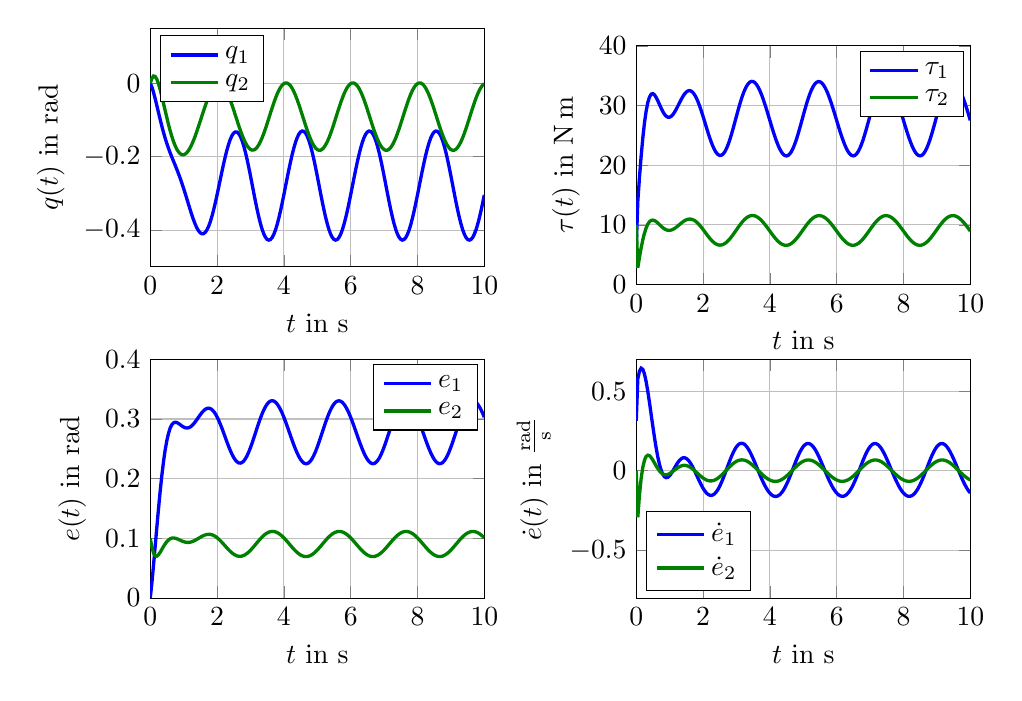
\begin{tikzpicture}

\begin{axis}[%
width=0.35\textwidth,
height=0.25\textwidth,
scale only axis,
xmin=0,
xmax=10,
xlabel={$t$ in $\mathrm{s}$},
xmajorgrids,
ymin=-0.5,
ymax=0.15,
ylabel={$q(t)$ in $\mathrm{rad}$},
ymajorgrids,
name=plot1,
legend style={at={(0.03,0.97)},anchor=north west,draw=black,fill=white,legend cell align=left}
]
\addplot [
color=blue,
solid,
line width=1.2pt
]
table[row sep=crcr]{
0 0\\
0.0466635464521439 -0.00915579321657421\\
0.0966635464521439 -0.0241206723596741\\
0.146663546452144 -0.0414643197518216\\
0.196663546452144 -0.0601742621918725\\
0.246663546452144 -0.0793707164550442\\
0.296663546452144 -0.0983362098904086\\
0.346663546452144 -0.116534488221546\\
0.396663546452144 -0.133613697335543\\
0.446663546452144 -0.149397287333023\\
0.496663546452144 -0.163865479494176\\
0.546663546452144 -0.17712976255877\\
0.596663546452144 -0.189402680018246\\
0.646663546452144 -0.200965040763087\\
0.696663546452144 -0.212132560858067\\
0.746663546452144 -0.223223781653843\\
0.796663546452144 -0.234530890127757\\
0.846663546452144 -0.246294790133301\\
0.896663546452145 -0.258685448349459\\
0.946663546452145 -0.271788182830322\\
0.996663546452145 -0.285596194890841\\
1.04666354645214 -0.300009287235511\\
1.09666354645213 -0.314838382739821\\
1.14666354645213 -0.329815177180014\\
1.19666354645212 -0.344606040115091\\
1.24666354645212 -0.358829130737066\\
1.29666354645211 -0.372073623257903\\
1.34666354645211 -0.383919935931646\\
1.3966635464521 -0.393959919475652\\
1.4466635464521 -0.401816070183719\\
1.49666354645209 -0.407158973997737\\
1.54666354645208 -0.409722344413922\\
1.59666354645208 -0.409315176516474\\
1.64666354645207 -0.40583069323077\\
1.69666354645207 -0.399251904205004\\
1.74666354645206 -0.389653732174056\\
1.79666354645206 -0.377201787364\\
1.84666354645205 -0.36214798793086\\
1.89666354645205 -0.344823331722779\\
1.94666354645204 -0.325628217023393\\
1.99666354645203 -0.305020780447804\\
2.04666354645203 -0.283503761670024\\
2.09666354645202 -0.261610412218952\\
2.14666354645202 -0.239889938573257\\
2.19666354645201 -0.218892913003311\\
2.24666354645201 -0.199157008912458\\
2.296663546452 -0.181193334103343\\
2.346663546452 -0.165473559652852\\
2.39666354645199 -0.152417986394395\\
2.44666354645199 -0.142384663841495\\
2.49666354645198 -0.135659680707535\\
2.54666354645197 -0.132448778869505\\
2.59666354645197 -0.132870494776709\\
2.64666354645196 -0.136951090248619\\
2.69666354645196 -0.144621581642267\\
2.74666354645195 -0.155717195151765\\
2.79666354645195 -0.169979551458138\\
2.84666354645194 -0.187061805466424\\
2.89666354645194 -0.206536835196869\\
2.94666354645193 -0.227908396960889\\
2.99666354645192 -0.250624960770026\\
3.04666354645192 -0.274095737141684\\
3.09666354645191 -0.29770823362055\\
3.14666354645191 -0.320846562815762\\
3.1966635464519 -0.342909680953175\\
3.2466635464519 -0.363328771307145\\
3.29666354645189 -0.38158309105495\\
3.34666354645189 -0.397213752462962\\
3.39666354645188 -0.409835083118829\\
3.44666354645188 -0.419143378567405\\
3.49666354645187 -0.424923003379798\\
3.54666354645186 -0.427049901965722\\
3.59666354645186 -0.425492647152615\\
3.64666354645185 -0.4203111899871\\
3.69666354645185 -0.411653490503613\\
3.74666354645184 -0.399750219077516\\
3.79666354645184 -0.384907731021759\\
3.84666354645183 -0.367499537457958\\
3.89666354645183 -0.347956521511197\\
3.94666354645182 -0.326756174354929\\
3.99666354645181 -0.304411142414014\\
4.04666354645183 -0.281457377912288\\
4.09666354645185 -0.258442166104424\\
4.14666354645186 -0.235912264862869\\
4.19666354645188 -0.214402341408461\\
4.2466635464519 -0.194423835967182\\
4.29666354645191 -0.176454333585783\\
4.34666354645193 -0.160927493127568\\
4.39666354645195 -0.148223573873233\\
4.44666354645196 -0.138660618513838\\
4.49666354645198 -0.132486395386669\\
4.546663546452 -0.129871266644805\\
4.59666354645201 -0.130902222515224\\
4.64666354645203 -0.135578391413711\\
4.69666354645205 -0.143808386063821\\
4.74666354645206 -0.155409861605598\\
4.79666354645208 -0.170111630288195\\
4.8466635464521 -0.187558591488271\\
4.89666354645211 -0.207319596310189\\
4.94666354645213 -0.22889818336102\\
4.99666354645215 -0.25174591628626\\
5.04666354645216 -0.275277850965145\\
5.09666354645218 -0.298889489729497\\
5.1466635464522 -0.321974466744688\\
5.19666354645221 -0.343942168744684\\
5.24666354645223 -0.364234531839323\\
5.29666354645225 -0.382341357980927\\
5.34666354645226 -0.397813643123476\\
5.39666354645228 -0.410274576864754\\
5.4466635464523 -0.419428034752644\\
5.49666354645231 -0.425064519741798\\
5.54666354645233 -0.427064608066386\\
5.59666354645235 -0.425400016536121\\
5.64666354645236 -0.420132440516814\\
5.69666354645238 -0.411410326664948\\
5.7466635464524 -0.399463754238596\\
5.79666354645241 -0.384597612670342\\
5.84666354645243 -0.367183284847915\\
5.89666354645245 -0.347649073266195\\
5.94666354645246 -0.326469633574018\\
5.99666354645248 -0.304154698845437\\
6.0466635464525 -0.281237380934059\\
6.09666354645251 -0.258262318656363\\
6.14666354645253 -0.235773907103448\\
6.19666354645255 -0.214304793570069\\
6.24666354645256 -0.194364772349999\\
6.29666354645258 -0.176430163427369\\
6.3466635464526 -0.160933728700017\\
6.39666354645261 -0.148255171072354\\
6.44666354645263 -0.138712279953445\\
6.49666354645265 -0.132552830239621\\
6.54666354645267 -0.129947404955466\\
6.59666354645268 -0.130983384351397\\
6.6466635464527 -0.135660413050224\\
6.69666354645272 -0.143887706501776\\
6.74666354645273 -0.155483573291459\\
6.79666354645275 -0.170177498087191\\
6.84666354645277 -0.187615043960568\\
6.89666354645278 -0.207365693277245\\
6.9466635464528 -0.228933563726184\\
6.99666354645282 -0.251770730124126\\
7.04666354645283 -0.275292680001497\\
7.09666354645285 -0.298895260440083\\
7.14666354645287 -0.321972360329131\\
7.19666354645288 -0.343933532107813\\
7.2466635464529 -0.364220793387436\\
7.29666354645292 -0.382323951504504\\
7.34666354645293 -0.397793942321176\\
7.39666354645295 -0.410253842229719\\
7.44666354645297 -0.419407373672444\\
7.49666354645298 -0.425044859839069\\
7.546663546453 -0.427046683094437\\
7.59666354645302 -0.42538436358407\\
7.64666354645303 -0.420119406887635\\
7.69666354645305 -0.411400084560383\\
7.74666354645307 -0.399456321296593\\
7.79666354645308 -0.384592876426982\\
7.8466635464531 -0.367181029311071\\
7.89666354645312 -0.3476490059707\\
7.94666354645313 -0.326471411720435\\
7.99666354645315 -0.304157953391593\\
8.04666354645313 -0.281241737795777\\
8.0966635464531 -0.258267416465533\\
8.14666354645307 -0.235779411251298\\
8.19666354645304 -0.214310406515066\\
8.24666354645301 -0.194370240379681\\
8.29666354645299 -0.176435280222413\\
8.34666354645296 -0.160938336153383\\
8.39666354645293 -0.148259157868567\\
8.4466635464529 -0.138715578419744\\
8.49666354645288 -0.132555411952017\\
8.54666354645285 -0.1299492755301\\
8.59666354645282 -0.13098457778631\\
8.64666354645279 -0.135660985914445\\
8.69666354645276 -0.143887732204836\\
8.74666354645274 -0.155483136611728\\
8.79666354645271 -0.170176690093759\\
8.84666354645268 -0.187613957430326\\
8.89666354645265 -0.207364418684287\\
8.94666354645263 -0.228932185861334\\
8.9966635464526 -0.251769325385078\\
9.04666354645257 -0.275291314375739\\
9.09666354645254 -0.298893988182012\\
9.14666354645252 -0.321971223309267\\
9.19666354645249 -0.343932559787154\\
9.24666354645246 -0.364220003346003\\
9.29666354645243 -0.382323350432726\\
9.3466635464524 -0.397793527368328\\
9.39666354645238 -0.410253602596647\\
9.44666354645235 -0.419407292336714\\
9.49666354645232 -0.425044915308704\\
9.54666354645229 -0.427046851099935\\
9.59666354645227 -0.425384618635514\\
9.64666354645224 -0.420119723642275\\
9.69666354645221 -0.411400438964545\\
9.74666354645218 -0.399456691482889\\
9.79666354645216 -0.384593243362896\\
9.84666354645213 -0.367181377207784\\
9.8966635464521 -0.347649322471331\\
9.94666354645207 -0.326471687894788\\
9.99666354645204 -0.304158183569963\\
};
\addlegendentry{$q_1$};

\addplot [
color=green!50!black,
solid,
line width=1.2pt
]
table[row sep=crcr]{
0 0\\
0.0466635464521439 0.0124130542433354\\
0.0966635464521439 0.0198395850371679\\
0.146663546452144 0.0188033431328314\\
0.196663546452144 0.011239005189147\\
0.246663546452144 -0.00118156862818231\\
0.296663546452144 -0.0170355583929673\\
0.346663546452144 -0.0351201812141119\\
0.396663546452144 -0.0544273385397241\\
0.446663546452144 -0.07412059489627\\
0.496663546452144 -0.0935141252296691\\
0.546663546452144 -0.112053549618253\\
0.596663546452144 -0.129298578908223\\
0.646663546452144 -0.144907364458919\\
0.696663546452144 -0.15862246031936\\
0.746663546452144 -0.170258360217581\\
0.796663546452144 -0.179690626954527\\
0.846663546452144 -0.186846654117073\\
0.896663546452145 -0.191698075094498\\
0.946663546452145 -0.194254769017666\\
0.996663546452145 -0.194560328233741\\
1.04666354645214 -0.192688771742077\\
1.09666354645213 -0.18874223283048\\
1.14666354645213 -0.18284932586536\\
1.19666354645212 -0.175163904966038\\
1.24666354645212 -0.165863956683244\\
1.29666354645211 -0.155150407638016\\
1.34666354645211 -0.143245666192296\\
1.3966635464521 -0.130391749494819\\
1.4466635464521 -0.116847874285531\\
1.49666354645209 -0.102887416486826\\
1.54666354645208 -0.0887941770769045\\
1.59666354645208 -0.0748579345822907\\
1.64666354645207 -0.0613693184491469\\
1.69666354645207 -0.0486140987342722\\
1.74666354645206 -0.036867048551925\\
1.79666354645206 -0.0263855875324468\\
1.84666354645205 -0.0174034491745577\\
1.89666354645205 -0.0101246275126128\\
1.94666354645204 -0.0047178483777307\\
1.99666354645203 -0.00131178131709373\\
2.04666354645203 8.83346892635934e-06\\
2.09666354645202 -0.000793984638182865\\
2.14666354645202 -0.00370975243549256\\
2.19666354645201 -0.00867898952564953\\
2.24666354645201 -0.0155938703062184\\
2.296663546452 -0.02430005240054\\
2.346663546452 -0.0345996535702645\\
2.39666354645199 -0.0462553313824485\\
2.44666354645199 -0.0589954006847967\\
2.49666354645198 -0.072519901465265\\
2.54666354645197 -0.0865075032409985\\
2.59666354645197 -0.100623102160431\\
2.64666354645196 -0.114525935045994\\
2.69666354645196 -0.127878003322373\\
2.74666354645195 -0.140352572921998\\
2.79666354645195 -0.151642498348228\\
2.84666354645194 -0.161468114591697\\
2.89666354645194 -0.169584452759703\\
2.94666354645193 -0.175787564678414\\
2.99666354645192 -0.17991978534004\\
3.04666354645192 -0.181873813290214\\
3.09666354645191 -0.181595539068767\\
3.14666354645191 -0.179085592103915\\
3.1966635464519 -0.174399601643421\\
3.2466635464519 -0.167647177279765\\
3.29666354645189 -0.158989614937513\\
3.34666354645189 -0.148636334362484\\
3.39666354645188 -0.13684006443166\\
3.44666354645188 -0.123890820315489\\
3.49666354645187 -0.110108763376497\\
3.54666354645186 -0.0958360959790587\\
3.59666354645186 -0.0814282093211573\\
3.64666354645185 -0.0672443609314648\\
3.69666354645185 -0.053638198614471\\
3.74666354645184 -0.0409484621727018\\
3.79666354645184 -0.0294901812189387\\
3.84666354645183 -0.019546650034544\\
3.89666354645183 -0.011362405881299\\
3.94666354645182 -0.00513737453687531\\
3.99666354645181 -0.00102228504948158\\
4.04666354645183 0.000884598155434471\\
4.09666354645185 0.000539419551538766\\
4.14666354645186 -0.0020466240921003\\
4.19666354645188 -0.00680790049008554\\
4.2466635464519 -0.0136261676378944\\
4.29666354645191 -0.0223335505092364\\
4.34666354645193 -0.0327166035392368\\
4.39666354645195 -0.0445213843027973\\
4.44666354645196 -0.0574594505989733\\
4.49666354645198 -0.0712146759693945\\
4.546663546452 -0.085450757902498\\
4.59666354645201 -0.0998192694497609\\
4.64666354645203 -0.113968080049213\\
4.69666354645205 -0.127549947093885\\
4.74666354645206 -0.14023105921348\\
4.79666354645208 -0.15169929918638\\
4.8466635464521 -0.161671992857544\\
4.89666354645211 -0.169902923393672\\
4.94666354645213 -0.176188418293044\\
4.99666354645215 -0.180372357092163\\
5.04666354645216 -0.182349994662905\\
5.09666354645218 -0.182070540334279\\
5.1466635464522 -0.179538469109537\\
5.19666354645221 -0.174813563319072\\
5.24666354645223 -0.168009691447037\\
5.29666354645225 -0.159292331117403\\
5.34666354645226 -0.148874844396693\\
5.39666354645228 -0.137013525179776\\
5.4466635464523 -0.124001467014215\\
5.49666354645231 -0.110161346412221\\
5.54666354645233 -0.0958372765905241\\
5.59666354645235 -0.0813859500850155\\
5.64666354645236 -0.0671673442904674\\
5.69666354645238 -0.0535353013462871\\
5.7466635464524 -0.0408283063098597\\
5.79666354645241 -0.0293607736117123\\
5.84666354645243 -0.0194151146518929\\
5.89666354645245 -0.0112348060210575\\
5.94666354645246 -0.00501861695003141\\
5.99666354645248 -0.000916094749664898\\
6.0466635464525 0.000975645100645765\\
6.09666354645251 0.000613818062169136\\
6.14666354645253 -0.00198941919614635\\
6.19666354645255 -0.00676760789963453\\
6.24666354645256 -0.013601825850575\\
6.29666354645258 -0.0223236689017536\\
6.3466635464526 -0.0327193113355288\\
6.39666354645261 -0.0445345717058641\\
6.44666354645263 -0.0574808974691542\\
6.49666354645265 -0.0712421645530358\\
6.54666354645267 -0.0854821672523069\\
6.59666354645268 -0.0998526503085271\\
6.6466635464527 -0.114001710043842\\
6.69666354645272 -0.127582367047788\\
6.74666354645273 -0.140261092176587\\
6.79666354645275 -0.151726054362159\\
6.84666354645277 -0.16169485695541\\
6.89666354645278 -0.169921542057109\\
6.9466635464528 -0.176202670176213\\
6.99666354645282 -0.180382322928063\\
7.04666354645283 -0.18235592334507\\
7.09666354645285 -0.182072813685589\\
7.14666354645287 -0.179537566692255\\
7.19666354645288 -0.174810028387139\\
7.2466635464529 -0.168004098966248\\
7.29666354645292 -0.159285258666442\\
7.34666354645293 -0.148866846677568\\
7.39666354645295 -0.137005112768656\\
7.44666354645297 -0.123993089839205\\
7.49666354645298 -0.110153382238268\\
7.546663546453 -0.0958300245318435\\
7.59666354645302 -0.0813796288811041\\
7.64666354645303 -0.067162094812715\\
7.69666354645305 -0.05353119258777\\
7.74666354645307 -0.0408253439790964\\
7.79666354645308 -0.0293589104130711\\
7.8466635464531 -0.0194142613842198\\
7.89666354645312 -0.0112348427415316\\
7.94666354645313 -0.00501940360476827\\
7.99666354645315 -0.000917480838619238\\
8.04666354645313 0.000973812101567201\\
8.0966635464531 0.000611685668072506\\
8.14666354645307 -0.00199171407772781\\
8.19666354645304 -0.00676994316003029\\
8.24666354645301 -0.0136040970408288\\
8.29666354645299 -0.0223257908735126\\
8.34666354645296 -0.0327212187958093\\
8.39666354645293 -0.044536218836405\\
8.4466635464529 -0.0574822567730274\\
8.49666354645288 -0.0712432250981579\\
8.54666354645285 -0.0854829324826624\\
8.59666354645282 -0.0998531355884523\\
8.64666354645279 -0.114001940088421\\
8.69666354645276 -0.12758237337389\\
8.74666354645274 -0.140260910685719\\
8.79666354645271 -0.151725723140056\\
8.84666354645268 -0.161694414346425\\
8.89666354645265 -0.16992102504612\\
8.94666354645263 -0.176202113088877\\
8.9966635464526 -0.180381756443141\\
9.04666354645257 -0.182355373800712\\
9.09666354645254 -0.182072302654739\\
9.14666354645252 -0.179537110799632\\
9.19666354645249 -0.174809639339942\\
9.24666354645246 -0.168003783771298\\
9.29666354645243 -0.159285020006324\\
9.3466635464524 -0.148866683416942\\
9.39666354645238 -0.137005020559267\\
9.44666354645235 -0.123993061789103\\
9.49666354645232 -0.110153409608562\\
9.54666354645229 -0.095830097424192\\
9.59666354645227 -0.0813797368817231\\
9.64666354645224 -0.0671622275641836\\
9.69666354645221 -0.0535313402676393\\
9.74666354645218 -0.0408254976732755\\
9.79666354645216 -0.0293590623808989\\
9.84666354645213 -0.0194144052199334\\
9.8966635464521 -0.0112349734427594\\
9.94666354645207 -0.00501951756237981\\
9.99666354645204 -0.000917575763877365\\
};
\addlegendentry{$q_2$};

\end{axis}

\begin{axis}[%
width=0.35\textwidth,
height=0.25\textwidth,
scale only axis,
xmin=0,
xmax=10,
xlabel={$t$ in $\mathrm{s}$},
xmajorgrids,
ymin=0,
ymax=0.4,
ylabel={$e(t)$ in $\mathrm{rad}$},
ymajorgrids,
name=plot3,
at=(plot1.below south west),
anchor=above north west,
legend style={draw=black,fill=white,legend cell align=left}
]
\addplot [
color=blue,
solid,
line width=1.2pt
]
table[row sep=crcr]{
0 0\\
0.0466635464521439 0.0237631263435458\\
0.0966635464521439 0.0540238161952011\\
0.146663546452144 0.0859269596518288\\
0.196663546452144 0.11810158039898\\
0.246663546452144 0.149336350145246\\
0.296663546452144 0.178617372959626\\
0.346663546452144 0.205154391997111\\
0.396663546452144 0.228390225673902\\
0.446663546452144 0.247996727561222\\
0.496663546452144 0.263859986161016\\
0.546663546452144 0.276057139047372\\
0.596663546452144 0.284827005998322\\
0.646663546452144 0.290536652633826\\
0.696663546452144 0.293645908264075\\
0.746663546452144 0.294671735454694\\
0.796663546452144 0.294154164578709\\
0.846663546452144 0.292625262339071\\
0.896663546452145 0.290582308322317\\
0.946663546452145 0.288466024018128\\
0.996663546452145 0.28664435349297\\
1.04666354645214 0.28540195410854\\
1.09666354645213 0.284935238904297\\
1.14666354645213 0.285352537280011\\
1.19666354645212 0.286678721907989\\
1.24666354645212 0.28886349704687\\
1.29666354645211 0.291792460188691\\
1.34666354645211 0.295300032156086\\
1.3966635464521 0.299183391137297\\
1.4466635464521 0.303216629955522\\
1.49666354645209 0.307164467330897\\
1.54666354645208 0.310794967925317\\
1.59666354645208 0.313890850536392\\
1.64666354645207 0.316259081360021\\
1.69666354645207 0.317738556798982\\
1.74666354645206 0.318205778373187\\
1.79666354645206 0.317578512913025\\
1.84666354645205 0.315817515725065\\
1.89666354645205 0.312926471749892\\
1.94666354645204 0.308950375835554\\
1.99666354645203 0.303972621845641\\
2.04666354645203 0.29811109479696\\
2.09666354645202 0.291513556054443\\
2.14666354645202 0.284352578473229\\
2.19666354645201 0.276820231210385\\
2.24666354645201 0.26912264260263\\
2.296663546452 0.261474497172534\\
2.346663546452 0.254093463428396\\
2.39666354645199 0.247194514732739\\
2.44666354645199 0.240984104069686\\
2.49666354645198 0.235654187374375\\
2.54666354645197 0.231376155358115\\
2.59666354645197 0.228294820756801\\
2.64666354645196 0.226522702119383\\
2.69666354645196 0.226134929048309\\
2.74666354645195 0.227165148952658\\
2.79666354645195 0.22960282590914\\
2.84666354645194 0.23339227767225\\
2.89666354645194 0.23843369516979\\
2.94666354645193 0.244586238148761\\
2.99666354645192 0.251673119372224\\
3.04666354645192 0.259488404014782\\
3.09666354645191 0.267805089785092\\
3.14666354645191 0.276383922915821\\
3.1966635464519 0.28498236274613\\
3.2466635464519 0.293363137616999\\
3.29666354645189 0.301301927985779\\
3.34666354645189 0.308593848687434\\
3.39666354645188 0.315058554780496\\
3.44666354645188 0.320543938339219\\
3.49666354645187 0.324928496712959\\
3.54666354645186 0.328122525477107\\
3.59666354645186 0.330068321172512\\
3.64666354645185 0.33073957811632\\
3.69666354645185 0.330140143097551\\
3.74666354645184 0.328302265276599\\
3.79666354645184 0.325284456570729\\
3.84666354645183 0.321169065252102\\
3.89666354645183 0.316059661538244\\
3.94666354645182 0.310078333167022\\
3.99666354645181 0.303362983811782\\
4.04666354645183 0.296064711039162\\
4.09666354645185 0.288345309939862\\
4.14666354645186 0.280374904762797\\
4.19666354645188 0.2723296596155\\
4.2466635464519 0.264389469657329\\
4.29666354645191 0.256735496654957\\
4.34666354645193 0.249547396903102\\
4.39666354645195 0.243000102211573\\
4.44666354645196 0.237260058742028\\
4.49666354645198 0.232480902053509\\
4.546663546452 0.228798643133414\\
4.59666354645201 0.226326548495312\\
4.64666354645203 0.225150003284465\\
4.69666354645205 0.225321733469846\\
4.74666354645206 0.226857815406466\\
4.79666354645208 0.229734904739164\\
4.8466635464521 0.233889063694054\\
4.89666354645211 0.239216456283056\\
4.94666354645213 0.24557602454883\\
4.99666354645215 0.252794074888388\\
5.04666354645216 0.260670517838167\\
5.09666354645218 0.268986345893959\\
5.1466635464522 0.277511826844666\\
5.19666354645221 0.286014850537559\\
5.24666354645223 0.294268898149102\\
5.29666354645225 0.302060194911689\\
5.34666354645226 0.309193739347893\\
5.39666354645228 0.31549804852638\\
5.4466635464523 0.320828594524437\\
5.49666354645231 0.325070013074958\\
5.54666354645233 0.328137231577793\\
5.59666354645235 0.329975690556064\\
5.64666354645236 0.330560828646106\\
5.69666354645238 0.329896979258983\\
5.7466635464524 0.328015800437801\\
5.79666354645241 0.324974338219457\\
5.84666354645243 0.320852812642226\\
5.89666354645245 0.315752213293427\\
5.94666354645246 0.309791792386311\\
5.99666354645248 0.303106540243414\\
6.0466635464525 0.29584471406114\\
6.09666354645251 0.288165462492001\\
6.14666354645253 0.280236547003564\\
6.19666354645255 0.27223211177728\\
6.24666354645256 0.264330406040295\\
6.29666354645258 0.256711326496668\\
6.3466635464526 0.249553632475648\\
6.39666354645261 0.243031699410761\\
6.44666354645263 0.237311720181671\\
6.49666354645265 0.232547336906463\\
6.54666354645267 0.228874781444044\\
6.59666354645268 0.226407710331422\\
6.6466635464527 0.225232024920886\\
6.69666354645272 0.22540105390768\\
6.74666354645273 0.22693152709218\\
6.79666354645275 0.229800772537992\\
6.84666354645277 0.233945516166164\\
6.89666354645278 0.239262553249914\\
6.9466635464528 0.245611404913787\\
6.99666354645282 0.252818888726044\\
7.04666354645283 0.260685346874311\\
7.09666354645285 0.268992116604345\\
7.14666354645287 0.277509720428921\\
7.19666354645288 0.286006213900516\\
7.2466635464529 0.294255159697065\\
7.29666354645292 0.302042788435141\\
7.34666354645293 0.309174038545496\\
7.39666354645295 0.315477313891279\\
7.44666354645297 0.320807933444201\\
7.49666354645298 0.325050353172226\\
7.546663546453 0.328119306605874\\
7.59666354645302 0.329960037604076\\
7.64666354645303 0.33054779501702\\
7.69666354645305 0.32988673715454\\
7.74666354645307 0.328008367495945\\
7.79666354645308 0.324969601976266\\
7.8466635464531 0.320850557105567\\
7.89666354645312 0.315752145998131\\
7.94666354645313 0.309793570532934\\
7.99666354645315 0.30310979478978\\
8.04666354645313 0.295849070923053\\
8.0966635464531 0.288170560301346\\
8.14666354645307 0.280242051151565\\
8.19666354645304 0.272237724722403\\
8.24666354645301 0.264335874070079\\
8.29666354645299 0.256716443291789\\
8.34666354645296 0.249558239929067\\
8.39666354645293 0.243035686207005\\
8.4466635464529 0.237315018647984\\
8.49666354645288 0.23254991861886\\
8.54666354645285 0.22887665201867\\
8.59666354645282 0.226408903766322\\
8.64666354645279 0.225232597785093\\
8.69666354645276 0.225401079610731\\
8.74666354645274 0.226931090412449\\
8.79666354645271 0.22979996454457\\
8.84666354645268 0.233944429635946\\
8.89666354645265 0.239261278656993\\
8.94666354645263 0.245610027048991\\
8.9966635464526 0.252817483987065\\
9.04666354645257 0.260683981248635\\
9.09666354645254 0.268990844346365\\
9.14666354645252 0.277508583409156\\
9.19666354645249 0.286005241579959\\
9.24666354645246 0.294254369655731\\
9.29666354645243 0.302042187363454\\
9.3466635464524 0.309173623592725\\
9.39666354645238 0.315477074258264\\
9.44666354645235 0.320807852108504\\
9.49666354645232 0.325050408641863\\
9.54666354645229 0.328119474611339\\
9.59666354645227 0.329960292655449\\
9.64666354645224 0.33054811177155\\
9.69666354645221 0.32988709155855\\
9.74666354645218 0.328008737682047\\
9.79666354645216 0.324969968911946\\
9.84666354645213 0.32085090500201\\
9.8966635464521 0.31575246249846\\
9.94666354645207 0.309793846706959\\
9.99666354645204 0.303110024967802\\
};
\addlegendentry{$e_1$};

\addplot [
color=green!50!black,
solid,
line width=1.2pt
]
table[row sep=crcr]{
0 0.1\\
0.0466635464521439 0.086514322245267\\
0.0966635464521439 0.075584740942908\\
0.146663546452144 0.0707682687379075\\
0.196663546452144 0.0702743422168608\\
0.246663546452144 0.072629522429033\\
0.296663546452144 0.0766588328439201\\
0.346663546452144 0.0814506534198813\\
0.396663546452144 0.0863241985125824\\
0.446663546452144 0.0907984360840763\\
0.496663546452144 0.0945622838317981\\
0.546663546452144 0.0974462164912813\\
0.596663546452144 0.0993954350726955\\
0.646663546452144 0.100444724558912\\
0.696663546452144 0.100695142112253\\
0.746663546452144 0.10029272652738\\
0.796663546452144 0.0994094638853089\\
0.846663546452144 0.0982267503415074\\
0.896663546452145 0.0969215467561379\\
0.946663546452145 0.0956553287894665\\
0.996663546452145 0.0945658215669009\\
1.04666354645214 0.0937613952534742\\
1.09666354645213 0.0933179068504036\\
1.14666354645213 0.0932777139946192\\
1.19666354645212 0.0936505575600263\\
1.24666354645212 0.0944160028823874\\
1.29666354645211 0.0955271331870547\\
1.34666354645211 0.0969151939865159\\
1.3966635464521 0.0984948895219475\\
1.4466635464521 0.10017003309771\\
1.49666354645209 0.10183925788468\\
1.54666354645208 0.103401510203858\\
1.59666354645208 0.104761078417798\\
1.64666354645207 0.105831958349134\\
1.69666354645207 0.10654141694136\\
1.74666354645206 0.106832682242108\\
1.79666354645206 0.106666750601648\\
1.84666354645205 0.106023352950109\\
1.89666354645205 0.104901155850962\\
1.94666354645204 0.103317288605925\\
1.99666354645203 0.101306287983934\\
2.04666354645203 0.0989185430196813\\
2.09666354645202 0.09621831061827\\
2.14666354645202 0.093281364306249\\
2.19666354645201 0.0901923369316811\\
2.24666354645201 0.0870418241070992\\
2.296663546452 0.0839233268515286\\
2.346663546452 0.080930125776075\\
2.39666354645199 0.0781521913553524\\
2.44666354645199 0.0756732418726521\\
2.49666354645198 0.0735680600674456\\
2.54666354645197 0.0719001701140795\\
2.59666354645197 0.0707199583249567\\
2.64666354645196 0.0700632951460372\\
2.69666354645196 0.0699506851153135\\
2.74666354645195 0.0703869392318392\\
2.79666354645195 0.0713613352790466\\
2.84666354645194 0.0728482108161611\\
2.89666354645194 0.0748079244213647\\
2.94666354645193 0.0771881244502256\\
2.99666354645192 0.0799252786732003\\
3.04666354645192 0.0829464368016016\\
3.09666354645191 0.0861712130886695\\
3.14666354645191 0.0895139802331429\\
3.1966635464519 0.0928862542373695\\
3.2466635464519 0.0961992234788599\\
3.29666354645189 0.0993663404864963\\
3.34666354645189 0.102305862156643\\
3.39666354645188 0.104943204458724\\
3.44666354645188 0.107212979127599\\
3.49666354645187 0.109060604774282\\
3.54666354645186 0.110443429105943\\
3.59666354645186 0.111331353156599\\
3.64666354645185 0.11170700083139\\
3.69666354645185 0.111565516821503\\
3.74666354645184 0.110914095862836\\
3.79666354645184 0.109771344288099\\
3.84666354645183 0.108166553810064\\
3.89666354645183 0.106138934219627\\
3.94666354645182 0.103736814765058\\
3.99666354645181 0.101016791716321\\
4.04666354645183 0.0980427783331823\\
4.09666354645185 0.0948849064285651\\
4.14666354645186 0.0916182359628784\\
4.19666354645188 0.0883212478961414\\
4.2466635464519 0.0850741214387995\\
4.29666354645191 0.0819568249602473\\
4.34666354645193 0.0790470757450657\\
4.39666354645195 0.0764182442757142\\
4.44666354645196 0.0741372917868355\\
4.49666354645198 0.072262834571575\\
4.546663546452 0.070843424775572\\
4.59666354645201 0.0699161256142729\\
4.64666354645203 0.0695054401492375\\
4.69666354645205 0.069622628886802\\
4.74666354645206 0.0702654255232963\\
4.79666354645208 0.0714181361171741\\
4.8466635464521 0.0730520890819861\\
4.89666354645211 0.0751263950553151\\
4.94666354645213 0.0775889780648447\\
4.99666354645215 0.0803778504253229\\
5.04666354645216 0.0834226181743031\\
5.09666354645218 0.0866462143542066\\
5.1466635464522 0.0899668572388059\\
5.19666354645221 0.0933002159130771\\
5.24666354645223 0.0965617376462054\\
5.29666354645225 0.0996690566664765\\
5.34666354645226 0.102544372190957\\
5.39666354645228 0.105116665206958\\
5.4466635464523 0.107323625826456\\
5.49666354645231 0.109113187810146\\
5.54666354645233 0.110444609717554\\
5.59666354645235 0.111289093920604\\
5.64666354645236 0.111629984190536\\
5.69666354645238 0.111462619553455\\
5.7466635464524 0.110793940000118\\
5.79666354645241 0.109641936680981\\
5.84666354645243 0.1080350184275\\
5.89666354645245 0.106011334359448\\
5.94666354645246 0.103618057178248\\
5.99666354645248 0.100910601416506\\
6.0466635464525 0.0979517313879404\\
6.09666354645251 0.0948105079178719\\
6.14666354645253 0.0915610310668312\\
6.19666354645255 0.0882809553055688\\
6.24666354645256 0.0850497796513334\\
6.29666354645258 0.0819469433525961\\
6.3466635464526 0.079049783541172\\
6.39666354645261 0.0764314316785822\\
6.44666354645263 0.0741587386568097\\
6.49666354645265 0.0722903231550065\\
6.54666354645267 0.0708748341251736\\
6.59666354645268 0.0699495064728389\\
6.6466635464527 0.0695390701436791\\
6.69666354645272 0.0696550488405342\\
6.74666354645273 0.0702954584862532\\
6.79666354645275 0.0714448912928278\\
6.84666354645277 0.0730749531797539\\
6.89666354645278 0.0751450137186856\\
6.9466635464528 0.0776032299479791\\
6.99666354645282 0.0803878162612201\\
7.04666354645283 0.0834285468564992\\
7.09666354645285 0.0866484877055792\\
7.14666354645287 0.0899659548216171\\
7.19666354645288 0.0932966809812653\\
7.2466635464529 0.0965561451655631\\
7.29666354645292 0.0996619842156836\\
7.34666354645293 0.102536374472018\\
7.39666354645295 0.105108252796037\\
7.44666354645297 0.107315248651654\\
7.49666354645298 0.109105223636402\\
7.546663546453 0.110437357659081\\
7.59666354645302 0.111282772716892\\
7.64666354645303 0.111624734712972\\
7.69666354645305 0.111458510795109\\
7.74666354645307 0.110790977669505\\
7.79666354645308 0.109640073482465\\
7.8466635464531 0.108034165159924\\
7.89666354645312 0.106011371079988\\
7.94666354645313 0.10361884383302\\
7.99666354645315 0.100911987505463\\
8.04666354645313 0.0979535643869901\\
8.0966635464531 0.0948126403119138\\
8.14666354645307 0.0915633259483375\\
8.19666354645304 0.0882832905658746\\
8.24666354645301 0.0850520508414883\\
8.29666354645299 0.0819490653242531\\
8.34666354645296 0.079051691001352\\
8.39666354645293 0.0764330788090288\\
8.4466635464529 0.0741600979605985\\
8.49666354645288 0.0722913837000572\\
8.54666354645285 0.0708755993554722\\
8.59666354645282 0.0699499917527228\\
8.64666354645279 0.0695393001882311\\
8.69666354645276 0.0696550551666238\\
8.74666354645274 0.0702952769953844\\
8.79666354645271 0.0714445600707328\\
8.84666354645268 0.073074510570782\\
8.89666354645265 0.075144496707709\\
8.94666354645263 0.0776026728606521\\
8.9966635464526 0.0803872497762994\\
9.04666354645257 0.0834279973121288\\
9.09666354645254 0.0866479766747008\\
9.14666354645252 0.0899654989289444\\
9.19666354645249 0.0932962919339966\\
9.24666354645246 0.096555829970517\\
9.29666354645243 0.0996617455554435\\
9.3466635464524 0.102536211211245\\
9.39666354645238 0.105108160586478\\
9.44666354645235 0.107315220601361\\
9.49666354645232 0.109105251006489\\
9.54666354645229 0.11043743055121\\
9.59666354645227 0.111282880717286\\
9.64666354645224 0.111624867464217\\
9.69666354645221 0.111458658474764\\
9.74666354645218 0.110791131363486\\
9.79666354645216 0.109640225450119\\
9.84666354645213 0.108034308995496\\
9.8966635464521 0.106011501781115\\
9.94666354645207 0.103618957790576\\
9.99666354645204 0.100912082430717\\
};
\addlegendentry{$e_2$};

\end{axis}

\begin{axis}[%
width=0.35\textwidth,
height=0.25\textwidth,
scale only axis,
xmin=0,
xmax=10,
xlabel={$t$ in $\mathrm{s}$},
xmajorgrids,
ymin=-0.8,
ymax=0.7,
ylabel={$\dot{e}(t)$ in $\mathrm{\frac{rad}{s}}$},
ymajorgrids,
name=plot2,
at=(plot3.right of south east),
anchor=left of south west,
legend style={at={(0.03,0.03)},anchor=south west,draw=black,fill=white,legend cell align=left}
]
\addplot [
color=blue,
solid,
line width=1.2pt
]
table[row sep=crcr]{
0 0.314159265358979\\
0.0466635464521439 0.578295306969531\\
0.0966635464521439 0.626150765110167\\
0.146663546452144 0.644652869603314\\
0.196663546452144 0.63723754145224\\
0.246663546452144 0.607465435597557\\
0.296663546452144 0.559612326486958\\
0.346663546452144 0.498297882370149\\
0.396663546452144 0.428185373604702\\
0.446663546452144 0.353740786625548\\
0.496663546452144 0.279042112330404\\
0.546663546452144 0.207634037622363\\
0.596663546452144 0.142425695289372\\
0.646663546452144 0.0856298543025435\\
0.696663546452144 0.0387415119083502\\
0.746663546452144 0.00255281428347987\\
0.796663546452144 -0.0227999964879911\\
0.846663546452144 -0.0377630474158256\\
0.896663546452145 -0.0432710187385706\\
0.946663546452145 -0.0406398640917704\\
0.996663546452145 -0.0314529961128685\\
1.04666354645214 -0.0174475784986259\\
1.09666354645213 -0.000406899153013784\\
1.14666354645213 0.017936195035385\\
1.19666354645212 0.035981062028449\\
1.24666354645212 0.0523238639488671\\
1.29666354645211 0.0658040204016636\\
1.34666354645211 0.0755327890771375\\
1.3966635464521 0.0809052646630555\\
1.4466635464521 0.0815978004506727\\
1.49666354645209 0.0775532528121884\\
1.54666354645208 0.0689565668917187\\
1.59666354645208 0.0562031414393082\\
1.64666354645207 0.0398622266824764\\
1.69666354645207 0.0206374060258016\\
1.74666354645206 -0.000673957854792878\\
1.79666354645206 -0.0232205615877302\\
1.84666354645205 -0.046134656180043\\
1.89666354645205 -0.0685657445521102\\
1.94666354645204 -0.089709309706755\\
1.99666354645203 -0.108829820614683\\
2.04666354645203 -0.125277801314079\\
2.09666354645202 -0.138501341393252\\
2.14666354645202 -0.14805297393636\\
2.19666354645201 -0.153593243335792\\
2.24666354645201 -0.154892444228093\\
2.296663546452 -0.151831891733859\\
2.346663546452 -0.14440569346702\\
2.39666354645199 -0.132723397642462\\
2.44666354645199 -0.117013189402672\\
2.49666354645198 -0.0976246200123464\\
2.54666354645197 -0.075029304001023\\
2.59666354645197 -0.0498177169283903\\
2.64666354645196 -0.022690252179197\\
2.69666354645196 0.00555891163034158\\
2.74666354645195 0.0340658351456126\\
2.79666354645195 0.0619284161849203\\
2.84666354645194 0.0882440877508053\\
2.89666354645194 0.112151045784\\
2.94666354645193 0.132869608914879\\
2.99666354645192 0.149739942207146\\
3.04666354645192 0.162252577744912\\
3.09666354645191 0.170068938969806\\
3.14666354645191 0.173030300518921\\
3.1966635464519 0.171155065554254\\
3.2466635464519 0.164625642105741\\
3.29666354645189 0.153767290185156\\
3.34666354645189 0.13902191452554\\
3.39666354645188 0.120919835786265\\
3.44666354645188 0.100052152457657\\
3.49666354645187 0.0770455688828326\\
3.54666354645186 0.0525407193148567\\
3.59666354645186 0.0271742599086246\\
3.64666354645185 0.00156446833000051\\
3.69666354645185 -0.023700160795305\\
3.74666354645184 -0.0480698361529386\\
3.79666354645184 -0.0710402573426672\\
3.84666354645183 -0.0921574216865913\\
3.89666354645183 -0.111020472531598\\
3.94666354645182 -0.127282620983659\\
3.99666354645181 -0.140650333852542\\
4.04666354645183 -0.150881248748033\\
4.09666354645185 -0.15778156979564\\
4.14666354645186 -0.161203918194693\\
4.19666354645188 -0.161046678337343\\
4.2466635464519 -0.15725574395976\\
4.29666354645191 -0.149829224932386\\
4.34666354645193 -0.138825161148642\\
4.39666354645195 -0.124371675655781\\
4.44666354645196 -0.106678374504947\\
4.49666354645198 -0.0860472623234511\\
4.546663546452 -0.0628810825365002\\
4.59666354645201 -0.0376868878665479\\
4.64666354645203 -0.0110728552441192\\
4.69666354645205 0.0162630996588997\\
4.74666354645206 0.0435535047232553\\
4.79666354645208 0.0699898322277157\\
4.8466635464521 0.0947576768948112\\
4.89666354645211 0.117075901353941\\
4.94666354645213 0.136236264366089\\
4.99666354645215 0.15163973777448\\
5.04666354645216 0.162825972523041\\
5.09666354645218 0.169493181346605\\
5.1466635464522 0.171506936057584\\
5.19666354645221 0.168897805123561\\
5.24666354645223 0.161849113150465\\
5.29666354645225 0.150677141088209\\
5.34666354645226 0.135806639829318\\
5.39666354645228 0.117744553479921\\
5.4466635464523 0.0970544147230335\\
5.49666354645231 0.0743331461748786\\
5.54666354645233 0.0501911813607715\\
5.59666354645235 0.02523609549308\\
5.64666354645236 5.94399650043764e-05\\
5.69666354645238 -0.0247737458634974\\
5.7466635464524 -0.0487332487325005\\
5.79666354645241 -0.0713301498383568\\
5.84666354645243 -0.0921215678509431\\
5.89666354645245 -0.110713662814863\\
5.94666354645246 -0.126762893745841\\
5.99666354645248 -0.139975680878934\\
6.0466635464525 -0.150106889440945\\
6.09666354645251 -0.156957843445953\\
6.14666354645253 -0.160374800280749\\
6.19666354645255 -0.160248887919424\\
6.24666354645256 -0.156518377910438\\
6.29666354645258 -0.149173833118502\\
6.3466635464526 -0.138266165615299\\
6.39666354645261 -0.123917035812432\\
6.44666354645263 -0.10633040756476\\
6.49666354645265 -0.0858035413533336\\
6.54666354645267 -0.0627353507470375\\
6.59666354645268 -0.0376299447000801\\
6.6466635464527 -0.011093385369573\\
6.69666354645272 0.0161777705725653\\
6.74666354645273 0.0434167343494367\\
6.79666354645275 0.0698150673444181\\
6.84666354645277 0.0945579394982158\\
6.89666354645278 0.116863354062724\\
6.9466635464528 0.136021855360977\\
6.99666354645282 0.151432926987189\\
7.04666354645283 0.162634541452525\\
7.09666354645285 0.169323128115202\\
7.14666354645287 0.171362454963691\\
7.19666354645288 0.168781346306974\\
7.2466635464529 0.161761513727065\\
7.29666354645292 0.150617815062254\\
7.34666354645293 0.13577381102526\\
7.39666354645295 0.117735514176051\\
7.44666354645297 0.0970657927933517\\
7.49666354645298 0.0743611651852287\\
7.546663546453 0.0502319008005828\\
7.59666354645302 0.0252856216237377\\
7.64666354645303 0.000114101130290784\\
7.69666354645305 -0.0247172625582371\\
7.74666354645307 -0.0486777999022409\\
7.79666354645308 -0.0712780759654055\\
7.8466635464531 -0.0920746680544149\\
7.89666354645312 -0.11067320004158\\
7.94666354645313 -0.1267296253405\\
7.99666354645315 -0.139949908940276\\
8.04666354645313 -0.150088525119955\\
8.0966635464531 -0.156946479416131\\
8.14666354645307 -0.160369786016698\\
8.19666354645304 -0.160249403130337\\
8.24666354645301 -0.156523500418164\\
8.29666354645299 -0.149182598542469\\
8.34666354645296 -0.138277617312624\\
8.39666354645293 -0.123930264513722\\
8.4466635464529 -0.10634458096297\\
8.49666354645288 -0.0858179244980564\\
8.54666354645285 -0.062749318459058\\
8.59666354645282 -0.0376429873700311\\
8.64666354645279 -0.0111051094808643\\
8.69666354645276 0.0161676460006983\\
8.74666354645274 0.04340838441251\\
8.79666354645271 0.0698085702343183\\
8.84666354645268 0.0945532872491467\\
8.89666354645265 0.116860464634572\\
8.94666354645263 0.136020585704523\\
8.9966635464526 0.151433086742549\\
9.04666354645257 0.162635906893177\\
9.09666354645254 0.169325455892741\\
9.14666354645252 0.171365495163402\\
9.19666354645249 0.16878485431687\\
9.24666354645246 0.161765260467681\\
9.29666354645243 0.150621595221919\\
9.3466635464524 0.135777449083434\\
9.39666354645238 0.117738868154781\\
9.44666354645235 0.0970687558301184\\
9.49666354645232 0.0743636651492361\\
9.54666354645229 0.0502338982657585\\
9.59666354645227 0.0252871065616048\\
9.64666354645224 0.0001150886980682\\
9.69666354645221 -0.0247167367754029\\
9.74666354645218 -0.0486776848710476\\
9.79666354645216 -0.0712783101268042\\
9.84666354645213 -0.09207518395748\\
9.8966635464521 -0.110673928506491\\
9.94666354645207 -0.126730499017088\\
9.99666354645204 -0.139950865177146\\
};
\addlegendentry{$\dot{e}_1$};

\addplot [
color=green!50!black,
solid,
line width=1.2pt
]
table[row sep=crcr]{
0 -0\\
0.0466635464521439 -0.29281600635641\\
0.0966635464521439 -0.151990254067377\\
0.146663546452144 -0.0485649075903094\\
0.196663546452144 0.0221761216676782\\
0.246663546452144 0.0665768033494602\\
0.296663546452144 0.0902407895486808\\
0.346663546452144 0.09810127238217\\
0.396663546452144 0.0944566431927068\\
0.446663546452144 0.0829959040586111\\
0.496663546452144 0.0668253422880044\\
0.546663546452144 0.0484984637946859\\
0.596663546452144 0.0300486228363747\\
0.646663546452144 0.0130241797312463\\
0.696663546452144 -0.00147306973588879\\
0.746663546452144 -0.012745131011166\\
0.796663546452144 -0.0204501292335795\\
0.846663546452144 -0.0245501056856703\\
0.896663546452145 -0.0252557217016572\\
0.946663546452145 -0.0229700122638572\\
0.996663546452145 -0.0182335435469715\\
1.04666354645214 -0.0116730646142014\\
1.09666354645213 -0.00395517301803278\\
1.14666354645213 0.00425413911467365\\
1.19666354645212 0.0123237355632542\\
1.24666354645212 0.0196853884254388\\
1.29666354645211 0.0258557467582061\\
1.34666354645211 0.0304523021907737\\
1.3966635464521 0.0332033708502222\\
1.4466635464521 0.0339521258643687\\
1.49666354645209 0.0326548626562428\\
1.54666354645208 0.0293739537748215\\
1.59666354645208 0.0242662892049305\\
1.64666354645207 0.0175683099931823\\
1.69666354645207 0.00957893841433238\\
1.74666354645206 0.000641729455440498\\
1.79666354645206 -0.00887259252325562\\
1.84666354645205 -0.0185823507965259\\
1.89666354645205 -0.0281093945865791\\
1.94666354645204 -0.0370916942101352\\
1.99666354645203 -0.0451941626310687\\
2.04666354645203 -0.0521179332618667\\
2.09666354645202 -0.0576083108926415\\
2.14666354645202 -0.0614615019425817\\
2.19666354645201 -0.0635300771984728\\
2.24666354645201 -0.0637269814542002\\
2.296663546452 -0.0620278224425845\\
2.346663546452 -0.058471166621492\\
2.39666354645199 -0.0531566408128726\\
2.44666354645199 -0.0462407704278378\\
2.49666354645198 -0.0379306538416571\\
2.54666354645197 -0.0284757535282761\\
2.59666354645197 -0.0181582531222632\\
2.64666354645196 -0.00728256053312759\\
2.69666354645196 0.00383539497415014\\
2.74666354645195 0.0148784417847035\\
2.79666354645195 0.0255375065772983\\
2.84666354645194 0.0355197061934594\\
2.89666354645194 0.0445551361410385\\
2.94666354645193 0.052402546186983\\
2.99666354645192 0.0588542537361082\\
3.04666354645192 0.0637406603552668\\
3.09666354645191 0.066934585104193\\
3.14666354645191 0.0683553461806645\\
3.1966635464519 0.067972198836278\\
3.2466635464519 0.0658064886507347\\
3.29666354645189 0.0619318075643105\\
3.34666354645189 0.0564715952970033\\
3.39666354645188 0.0495939866800664\\
3.44666354645188 0.0415041737253289\\
3.49666354645187 0.0324350004483275\\
3.54666354645186 0.0226368147637529\\
3.59666354645186 0.0123676856887174\\
3.64666354645185 0.00188494128001243\\
3.69666354645185 -0.00856135767686983\\
3.74666354645184 -0.018732828894676\\
3.79666354645184 -0.0284053101972876\\
3.84666354645183 -0.0373700991155451\\
3.89666354645183 -0.0454346198569591\\
3.94666354645182 -0.0524232332493923\\
3.99666354645181 -0.058178740309333\\
4.04666354645183 -0.0625648669960463\\
4.09666354645185 -0.0654697223200504\\
4.14666354645186 -0.066809956529762\\
4.19666354645188 -0.0665351561320248\\
4.2466635464519 -0.0646319198762743\\
4.29666354645191 -0.0611270631144724\\
4.34666354645193 -0.056089478888242\\
4.39666354645195 -0.049630317112921\\
4.44666354645196 -0.0419013040660038\\
4.49666354645198 -0.0330911947979849\\
4.546663546452 -0.0234205184454467\\
4.59666354645201 -0.0131349295332686\\
4.64666354645203 -0.00249760250865766\\
4.69666354645205 0.00821881815359299\\
4.74666354645206 0.0187401957885787\\
4.79666354645208 0.028798372149176\\
4.8466635464521 0.0381378580428665\\
4.89666354645211 0.0465216835453304\\
4.94666354645213 0.0537365526656037\\
4.99666354645215 0.0595975772215375\\
5.04666354645216 0.0639528630010371\\
5.09666354645218 0.0666880698915541\\
5.1466635464522 0.0677308018841814\\
5.19666354645221 0.0670543873385645\\
5.24666354645223 0.0646803930420149\\
5.29666354645225 0.0606791709366177\\
5.34666354645226 0.0551679061455928\\
5.39666354645228 0.0483059913143223\\
5.4466635464523 0.0402880046580996\\
5.49666354645231 0.0313349941175726\\
5.54666354645233 0.0216850523079837\\
5.59666354645235 0.0115842347858511\\
5.64666354645236 0.00127871788195949\\
5.69666354645238 -0.0089912384582726\\
5.7466635464524 -0.0189953737549036\\
5.79666354645241 -0.0285158082680481\\
5.84666354645243 -0.0373482750902869\\
5.89666354645245 -0.0453029017716839\\
5.94666354645246 -0.0522052188531236\\
5.99666354645248 -0.0578979080611441\\
6.0466635464525 -0.0622435460019077\\
6.09666354645251 -0.0651283129728922\\
6.14666354645253 -0.0664663804868223\\
6.19666354645255 -0.0662045088003976\\
6.24666354645256 -0.0643262980644452\\
6.29666354645258 -0.0608555422447256\\
6.3466635464526 -0.0558582161396631\\
6.39666354645261 -0.0494427580289963\\
6.44666354645263 -0.041758470355319\\
6.49666354645265 -0.032992030718595\\
6.54666354645267 -0.0233622729683102\\
6.59666354645268 -0.0131135520395306\\
6.6466635464527 -0.00250813145711581\\
6.69666354645272 0.00818189127966368\\
6.74666354645273 0.0186826010737495\\
6.79666354645275 0.0287257836957102\\
6.84666354645277 0.0380556689335465\\
6.89666354645278 0.0464348336346653\\
6.9466635464528 0.053649405941383\\
6.99666354645282 0.059513843013507\\
7.04666354645283 0.0638755541329378\\
7.09666354645285 0.0666194909356923\\
7.14666354645287 0.0676725617088045\\
7.19666354645288 0.0670074316712509\\
7.2466635464529 0.0646450542582315\\
7.29666354645292 0.0606552332385806\\
7.34666354645293 0.0551546844461075\\
7.39666354645295 0.0483024214926444\\
7.44666354645297 0.0402927416909235\\
7.49666354645298 0.0313465133570107\\
7.546663546453 0.0217017483429913\\
7.59666354645302 0.0116045122135348\\
7.64666354645303 0.00130106903602184\\
7.69666354645305 -0.00896817235184427\\
7.74666354645307 -0.0189727596995415\\
7.79666354645308 -0.0284945967387526\\
7.8466635464531 -0.0373291916683594\\
7.89666354645312 -0.0452864523764034\\
7.94666354645313 -0.0521917052791742\\
7.99666354645315 -0.0578874505467114\\
8.04666354645313 -0.0622361099344642\\
8.0966635464531 -0.0651237374107865\\
8.14666354645307 -0.0664644067759806\\
8.19666354645304 -0.0662048080860857\\
8.24666354645301 -0.064328496886968\\
8.29666354645299 -0.0608592456656077\\
8.34666354645296 -0.0558630280046605\\
8.39666354645293 -0.0494482980816374\\
8.4466635464529 -0.0417643880095416\\
8.49666354645288 -0.0329980154058456\\
8.54666354645285 -0.0233680611001184\\
8.59666354645282 -0.0131189307637189\\
8.64666354645279 -0.00251293951928699\\
8.69666354645276 0.00817776514476043\\
8.74666354645274 0.0186792217178228\\
8.79666354645271 0.0287231745607237\\
8.84666354645268 0.0380538179546348\\
8.89666354645265 0.0464336995645281\\
8.94666354645263 0.0536489247027416\\
8.9966635464526 0.0595139337898141\\
9.04666354645257 0.063876125014148\\
9.09666354645254 0.0666204440289836\\
9.14666354645252 0.0676737976900929\\
9.19666354645249 0.0670088537854022\\
9.24666354645246 0.0646465717757018\\
9.29666354645243 0.0606567643543025\\
9.3466635464524 0.0551561585783013\\
9.39666354645238 0.0483037809213658\\
9.44666354645235 0.0402939424801337\\
9.49666354645232 0.0313475255334687\\
9.54666354645229 0.0217025553551081\\
9.59666354645227 0.0116051097519441\\
9.64666354645224 0.00130146335091758\\
9.69666354645221 -0.00896796646553893\\
9.74666354645218 -0.0189727210661049\\
9.79666354645216 -0.0284946999440635\\
9.84666354645213 -0.0373294090417678\\
9.8966635464521 -0.0452867557155961\\
9.94666354645207 -0.0521920672657874\\
9.99666354645204 -0.0578878458390978\\
};
\addlegendentry{$\dot{e}_2$};

\end{axis}

\begin{axis}[%
width=0.35\textwidth,
height=0.25\textwidth,
scale only axis,
xmin=0,
xmax=10,
xlabel={$t$ in $\mathrm{s}$},
xmajorgrids,
ymin=0,
ymax=40,
ylabel={$\tau(t)$ in $\mathrm{N\,m}$},
ymajorgrids,
at=(plot2.above north west),
anchor=below south west,
legend style={draw=black,fill=white,legend cell align=left}
]
\addplot [
color=blue,
solid,
line width=1.2pt
]
table[row sep=crcr]{
0 6.28318530717959\\
0.0466635464521439 13.9452141602671\\
0.0966635464521439 17.9314938093825\\
0.146663546452144 21.4948016204368\\
0.196663546452144 24.5666857093899\\
0.246663546452144 27.0971591592855\\
0.296663546452144 29.07028781974\\
0.346663546452144 30.4993879439377\\
0.396663546452144 31.4219652385804\\
0.446663546452144 31.8944941555622\\
0.496663546452144 31.9871243915568\\
0.546663546452144 31.7784566001523\\
0.596663546452144 31.3505608710905\\
0.646663546452144 30.7844167656826\\
0.696663546452144 30.1559365096227\\
0.746663546452144 29.5326996399176\\
0.796663546452144 28.9714844059056\\
0.846663546452144 28.5166340811985\\
0.896663546452145 28.1992494800406\\
0.946663546452145 28.0371558194242\\
0.996663546452145 28.0355552980123\\
1.04666354645214 28.1882484543597\\
1.09666354645213 28.4792890197104\\
1.14666354645213 28.8849293655211\\
1.19666354645212 29.3757165909207\\
1.24666354645212 29.9186115508547\\
1.29666354645211 30.4790224328642\\
1.34666354645211 31.0226679003278\\
1.3966635464521 31.5172092078947\\
1.4466635464521 31.9336133376366\\
1.49666354645209 32.2472282604864\\
1.54666354645208 32.4385661873982\\
1.59666354645208 32.4938015169545\\
1.64666354645207 32.4049982534025\\
1.69666354645207 32.170088355366\\
1.74666354645206 31.7926288714442\\
1.79666354645206 31.2813721817535\\
1.84666354645205 30.6496896532977\\
1.89666354645205 29.9148932613667\\
1.94666354645204 29.0975006899735\\
1.99666354645203 28.2204859012978\\
2.04666354645203 27.3085488399363\\
2.09666354645202 26.3874256652383\\
2.14666354645202 25.4832466317833\\
2.19666354645201 24.6219350947698\\
2.24666354645201 23.8286308085108\\
2.296663546452 23.1271158766144\\
2.346663546452 22.5392235703228\\
2.39666354645199 22.0842187195208\\
2.44666354645199 21.7781522858442\\
2.49666354645198 21.6332098660377\\
2.54666354645197 21.6570913987589\\
2.59666354645197 21.8524741025832\\
2.64666354645196 22.2166195846035\\
2.69666354645196 22.741186582486\\
2.74666354645195 23.4123014069567\\
2.79666354645195 24.2109187924069\\
2.84666354645194 25.113478317849\\
2.89666354645194 26.0928294552393\\
2.94666354645193 27.1193666926205\\
2.99666354645192 28.162290652338\\
3.04666354645192 29.1908965698546\\
3.09666354645191 30.1757908702463\\
3.14666354645191 31.0899500387729\\
3.1966635464519 31.9095607452509\\
3.2466635464519 32.614611171005\\
3.29666354645189 33.1892346082429\\
3.34666354645189 33.6218320624306\\
3.39666354645188 33.9050169946788\\
3.44666354645188 34.035431216146\\
3.49666354645187 34.0134775201054\\
3.54666354645186 33.84300499104\\
3.59666354645186 33.5309709499528\\
3.64666354645185 33.087092761983\\
3.69666354645185 32.5234956488008\\
3.74666354645184 31.8543599958224\\
3.79666354645184 31.0955726324251\\
3.84666354645183 30.2643892958704\\
3.89666354645183 29.3791176806121\\
3.94666354645182 28.4588301975822\\
3.99666354645181 27.5231118331547\\
4.04666354645183 26.5918415154774\\
4.09666354645185 25.6849964857324\\
4.14666354645186 24.8224603755735\\
4.19666354645188 24.0238092352503\\
4.2466635464519 23.3080475193474\\
4.29666354645191 22.6932691608862\\
4.34666354645193 22.196227564161\\
4.39666354645195 21.8318119071378\\
4.44666354645196 21.6124440510329\\
4.49666354645198 21.547428487729\\
4.546663546452 21.6423046055792\\
4.59666354645201 21.8982634576711\\
4.64666354645203 22.3116976398133\\
4.69666354645205 22.8739507852109\\
4.74666354645206 23.5713214438904\\
4.79666354645208 24.3853549962652\\
4.8466635464521 25.2934287029095\\
4.89666354645211 26.2696026779647\\
4.94666354645213 27.2856784416516\\
4.99666354645215 28.312382115301\\
5.04666354645216 29.3205758477557\\
5.09666354645218 30.282401328669\\
5.1466635464522 31.1722731424306\\
5.19666354645221 31.96766431578\\
5.24666354645223 32.6496566451098\\
5.29666354645225 33.2032583188949\\
5.34666354645226 33.6175156345521\\
5.39666354645228 33.8854607231403\\
5.4466635464523 34.0039420799753\\
5.49666354645231 33.9733807021462\\
5.54666354645233 33.7974848420269\\
5.59666354645235 33.4829445999971\\
5.64666354645236 33.0391172476616\\
5.69666354645238 32.4777075635801\\
5.7466635464524 31.8124452603514\\
5.79666354645241 31.0587629473842\\
5.84666354645243 30.2334811115958\\
5.89666354645245 29.3545090504652\\
5.94666354645246 28.4405706642675\\
5.99666354645248 27.5109605357901\\
6.0466635464525 26.585329003817\\
6.09666354645251 25.6834862679401\\
6.14666354645253 24.8252069579291\\
6.19666354645255 24.0300102597867\\
6.24666354645256 23.3168884786304\\
6.29666354645258 22.703959981335\\
6.3466635464526 22.2080310320824\\
6.39666354645261 21.8440644239236\\
6.44666354645263 21.6245695338009\\
6.49666354645265 21.5589463924268\\
6.54666354645267 21.6528330724315\\
6.59666354645268 21.9075185046115\\
6.6466635464527 22.3194892009462\\
6.69666354645272 22.8801762472676\\
6.74666354645273 23.5759572049854\\
6.79666354645275 24.388446478482\\
6.84666354645277 25.2950792021886\\
6.89666354645278 26.2699614288261\\
6.9466635464528 27.284928298045\\
6.99666354645282 28.3107272833208\\
7.04666354645283 29.3182301299597\\
7.09666354645285 30.2795773350795\\
7.14666354645287 31.1691728789782\\
7.19666354645288 31.9644714757439\\
7.2466635464529 32.646530811438\\
7.29666354645292 33.200331150721\\
7.34666354645293 33.6148889782312\\
7.39666354645295 33.8832064735527\\
7.44666354645297 34.0021035333581\\
7.49666354645298 33.9719750920801\\
7.546663546453 33.7965067336312\\
7.59666354645302 33.4823698274115\\
7.64666354645303 33.0389071080588\\
7.69666354645305 32.477813019241\\
7.74666354645307 31.8128109427711\\
7.79666354645308 31.0593308005241\\
7.8466635464531 30.2341935538606\\
7.89666354645312 29.3553115764013\\
7.94666354645313 28.4414138470367\\
7.99666354645315 27.5118014291999\\
8.04666354645313 26.5861319764281\\
8.0966635464531 25.684223329471\\
8.14666354645307 24.8258576580103\\
8.19666354645304 24.0305612500808\\
8.24666354645301 23.3173328314543\\
8.29666354645299 22.7042963523677\\
8.34666354645296 22.2082627434778\\
8.39666354645293 21.8441985295222\\
8.4466635464529 21.624615912468\\
8.49666354645288 21.558916900772\\
8.54666354645285 21.6527407756536\\
8.59666354645282 21.9073769947024\\
8.64666354645279 22.3193120051411\\
8.69666354645276 22.8799763261353\\
8.74666354645274 23.5757465382737\\
8.79666354645271 24.3882357369378\\
8.84666354645268 25.2948775041854\\
8.89666354645265 26.269776180971\\
8.94666354645263 27.2847651184364\\
8.9966635464526 28.3105900045301\\
9.04666354645257 29.3181208762051\\
9.09666354645254 30.2794966648323\\
9.14666354645252 31.1691199809959\\
9.19666354645249 31.9644444038862\\
9.24666354645246 32.646526742117\\
9.29666354645243 33.2003466467456\\
9.3466635464524 33.6149202441176\\
9.39666354645238 33.8832495898258\\
9.44666354645235 34.0021546605237\\
9.49666354645232 33.9720306383239\\
9.54666354645229 33.7965634834813\\
9.59666354645227 33.4824250313062\\
9.64666354645224 33.0389585348672\\
9.69666354645221 32.4778589752987\\
9.74666354645218 31.812850262005\\
9.79666354645216 31.0593628108641\\
9.84666354645213 30.2342180254435\\
9.8966635464521 29.3553286571359\\
9.94666354645207 28.4414239909074\\
9.99666354645204 27.5118053222646\\
};
\addlegendentry{$\tau_1$};

\addplot [
color=green!50!black,
solid,
line width=1.2pt
]
table[row sep=crcr]{
0 10\\
0.0466635464521439 2.8151740403663\\
0.0966635464521439 4.53801537841411\\
0.146663546452144 6.12368313823366\\
0.196663546452144 7.48747210008789\\
0.246663546452144 8.60895811867119\\
0.296663546452144 9.48276695316007\\
0.346663546452144 10.1164595852394\\
0.396663546452144 10.5279917376926\\
0.446663546452144 10.7431123890267\\
0.496663546452144 10.7929150999125\\
0.546663546452144 10.7115955385\\
0.596663546452144 10.534419076338\\
0.646663546452144 10.2959077873285\\
0.696663546452144 10.0282759760603\\
0.746663546452144 9.76015459970493\\
0.796663546452144 9.51563980982111\\
0.846663546452144 9.31368182361374\\
0.896663546452145 9.16780504248447\\
0.946663546452145 9.08612696674046\\
0.996663546452145 9.07162775690354\\
1.04666354645214 9.12261629009559\\
1.09666354645213 9.23334085920886\\
1.14666354645213 9.39469976550629\\
1.19666354645212 9.59501502221947\\
1.24666354645212 9.82083824796884\\
1.29666354645211 10.0577603760751\\
1.34666354645211 10.2911966468592\\
1.3966635464521 10.5071173466189\\
1.4466635464521 10.6926951276115\\
1.49666354645209 10.8368431706202\\
1.54666354645208 10.930625482404\\
1.59666354645208 10.9675305135375\\
1.64666354645207 10.9436102979647\\
1.69666354645207 10.8574973028698\\
1.74666354645206 10.7103182461294\\
1.79666354645206 10.5055272037379\\
1.84666354645205 10.248679375904\\
1.89666354645205 9.94716289246084\\
1.94666354645204 9.60990064331883\\
1.99666354645203 9.24702907461912\\
2.04666354645203 8.8695575796986\\
2.09666354645202 8.48901120944502\\
2.14666354645202 8.11706080802237\\
2.19666354645201 7.7651475942469\\
2.24666354645201 7.4441125904046\\
2.296663546452 7.16384411409562\\
2.346663546452 6.93295804078558\\
2.39666354645199 6.75852534185807\\
2.44666354645199 6.64585947815528\\
2.49666354645198 6.59837280088406\\
2.54666354645197 6.61750655432059\\
2.59666354645197 6.70273388239138\\
2.64666354645196 6.85163004075352\\
2.69666354645196 7.05999957056723\\
2.74666354645195 7.32204732606829\\
2.79666354645195 7.63057966541244\\
2.84666354645194 7.97722410866171\\
2.89666354645194 8.35265996586107\\
2.94666354645193 8.74685770183318\\
2.99666354645192 9.14932941319506\\
3.04666354645192 9.54939494429769\\
3.09666354645191 9.93646664547996\\
3.14666354645191 10.3003505306785\\
3.1966635464519 10.6315539554143\\
3.2466635464519 10.921582312122\\
3.29666354645189 11.1632023221414\\
3.34666354645189 11.3506493259964\\
3.39666354645188 11.4797611568934\\
3.44666354645188 11.5480306878197\\
3.49666354645187 11.5545806154221\\
3.54666354645186 11.5000745923912\\
3.59666354645186 11.3865859170933\\
3.64666354645185 11.2174471719269\\
3.69666354645185 10.99710136906\\
3.74666354645184 10.7309684411998\\
3.79666354645184 10.4253322189023\\
3.84666354645183 10.087244495519\\
3.89666354645183 9.72443622391965\\
3.94666354645182 9.34522247844699\\
3.99666354645181 8.95838789429255\\
4.04666354645183 8.57304243636513\\
4.09666354645185 8.19844256192637\\
4.14666354645186 7.84377888194172\\
4.19666354645188 7.51793711202191\\
4.2466635464519 7.22924355513316\\
4.29666354645191 6.98520911152974\\
4.34666354645193 6.79228679234965\\
4.39666354645195 6.65565710789328\\
4.44666354645196 6.57905379681029\\
4.49666354645198 6.56463943217044\\
4.546663546452 6.61293672212643\\
4.59666354645201 6.72281708310288\\
4.64666354645203 6.89154370156294\\
4.69666354645205 7.11486241130493\\
4.74666354645206 7.38713103529149\\
4.79666354645208 7.70147706066273\\
4.8466635464521 8.04997497223234\\
4.89666354645211 8.42383797734193\\
4.94666354645213 8.81362319286749\\
4.99666354645215 9.2094530581159\\
5.04666354645216 9.60125713448324\\
5.09666354645218 9.9790364677809\\
5.1466635464522 10.3331473453151\\
5.19666354645221 10.6545938930308\\
5.24666354645223 10.9353118166822\\
5.29666354645225 11.1684212075856\\
5.34666354645226 11.3484265463996\\
5.39666354645228 11.471347324402\\
5.4466635464523 11.5347719763608\\
5.49666354645231 11.5378387923934\\
5.54666354645233 11.4811574044369\\
5.59666354645235 11.3666909754364\\
5.64666354645236 11.1976210398805\\
5.69666354645238 10.9782140266272\\
5.7466635464524 10.7137019577235\\
5.79666354645241 10.4101814967753\\
5.84666354645243 10.0745274377679\\
5.89666354645245 9.71431059960726\\
5.94666354645246 9.33770700769137\\
5.99666354645248 8.95338550927489\\
6.0466635464525 8.5703641617237\\
6.09666354645251 8.1978308978002\\
6.14666354645253 7.84492991319578\\
6.19666354645255 7.52052079959716\\
6.24666354645256 7.2329218126231\\
6.29666354645258 6.98965136815952\\
6.3466635464526 6.79718282693183\\
6.39666354645261 6.66072702985853\\
6.44666354645263 6.58405515802137\\
6.49666354645265 6.56937157210134\\
6.54666354645267 6.61724256662927\\
6.59666354645268 6.7265827188342\\
6.6466635464527 6.8946961220379\\
6.69666354645272 7.11736586919953\\
6.74666354645273 7.38898243729059\\
6.79666354645275 7.70270080915877\\
6.84666354645277 8.0506175998227\\
6.89666354645278 8.42396284546567\\
6.9466635464528 8.81330544669651\\
6.99666354645282 9.20877495754502\\
7.04666354645283 9.60030382534087\\
7.09666354645285 9.97789222380092\\
7.14666354645287 10.3318923000887\\
7.19666354645288 10.6533012865033\\
7.2466635464529 10.9340457929423\\
7.29666354645292 11.1672352085456\\
7.34666354645293 11.3473623405161\\
7.39666354645295 11.4704346868763\\
7.44666354645297 11.5340289995371\\
7.49666354645298 11.5372727598078\\
7.546663546453 11.4807661192898\\
7.59666354645302 11.366464403619\\
7.64666354645303 11.1975431152054\\
7.69666354645305 10.9782644729212\\
7.74666354645307 10.7138580057694\\
7.79666354645308 10.4104194075096\\
7.8466635464531 10.0748237794488\\
7.89666354645312 9.71464325956698\\
7.94666354645313 9.33805594464755\\
7.99666354645315 8.9537332684592\\
8.04666354645313 8.57069618297751\\
8.0966635464531 8.19813564844648\\
8.14666354645307 7.8451988755632\\
8.19666354645304 7.52074833991395\\
8.24666354645301 7.2331049551881\\
8.29666354645299 6.98978949690754\\
8.34666354645296 6.79727733564985\\
8.39666354645293 6.66078094185035\\
8.4466635464529 6.58407273531578\\
8.49666354645288 6.56935793286139\\
8.54666354645285 6.61720332702297\\
8.59666354645282 6.72652367233881\\
8.64666354645279 6.89462296524968\\
8.69666354645276 7.11728397911044\\
8.74666354645274 7.38889670108517\\
8.79666354645271 7.70261550424954\\
8.84666354645268 8.05053631934729\\
8.89666354645265 8.42388846296529\\
8.94666354645263 8.813240113191\\
8.9966635464526 9.20872012457909\\
9.04666354645257 9.60026028852805\\
9.09666354645254 9.97786018257892\\
9.14666354645252 10.3318714304472\\
9.19666354645249 10.6532908240595\\
9.24666354645246 10.9340446237871\\
9.29666354645243 11.167241964836\\
9.3466635464524 11.3473754970826\\
9.39666354645238 11.4704526544948\\
9.44666354645235 11.5340502102919\\
9.49666354645232 11.5372957403456\\
9.54666354645229 11.480789548745\\
9.59666354645227 11.3664871544266\\
9.64666354645224 11.1975642766277\\
9.69666354645221 10.9782833586127\\
9.74666354645218 10.7138741478362\\
9.79666354645216 10.4104325401688\\
9.84666354645213 10.0748338155378\\
9.8966635464521 9.71465026289569\\
9.94666354645207 9.33806010067085\\
9.99666354645204 8.95373485513691\\
};
\addlegendentry{$\tau_2$};

\end{axis}
\end{tikzpicture}%
	\caption{Simulation results of classical PD controller with $\omega_n = 10\,\mathrm{\frac{rad}{s}}$}
	\label{fig:ch3_sim21}
\end{figure}
Figure \ref{fig:ch3_sim22} shows the simulation results for the decoupled PD controller with $\omega_n = 25\,\mathrm{\frac{rad}{s}}$. Compared to the previous results, with the lower gains, the position error is smaller with an average value of $0.05\,\mathrm{rad}$ for the first joint and $0.19\,\mathrm{rad}$ for the second joint. The amplitude of the velocity error is also smaller than in the previous simulation. On the other hand, the initial torque already shows a high peak of approximately $60\,\mathrm{N\,m}$. After the system is settled, the amplitudes of the torque are similar to the previous simulation.
\begin{figure}[H]
	\centering
	% This file was created by matlab2tikz v0.4.3.
% Copyright (c) 2008--2013, Nico Schlömer <nico.schloemer@gmail.com>
% All rights reserved.
% 
% The latest updates can be retrieved from
%   http://www.mathworks.com/matlabcentral/fileexchange/22022-matlab2tikz
% where you can also make suggestions and rate matlab2tikz.
% 
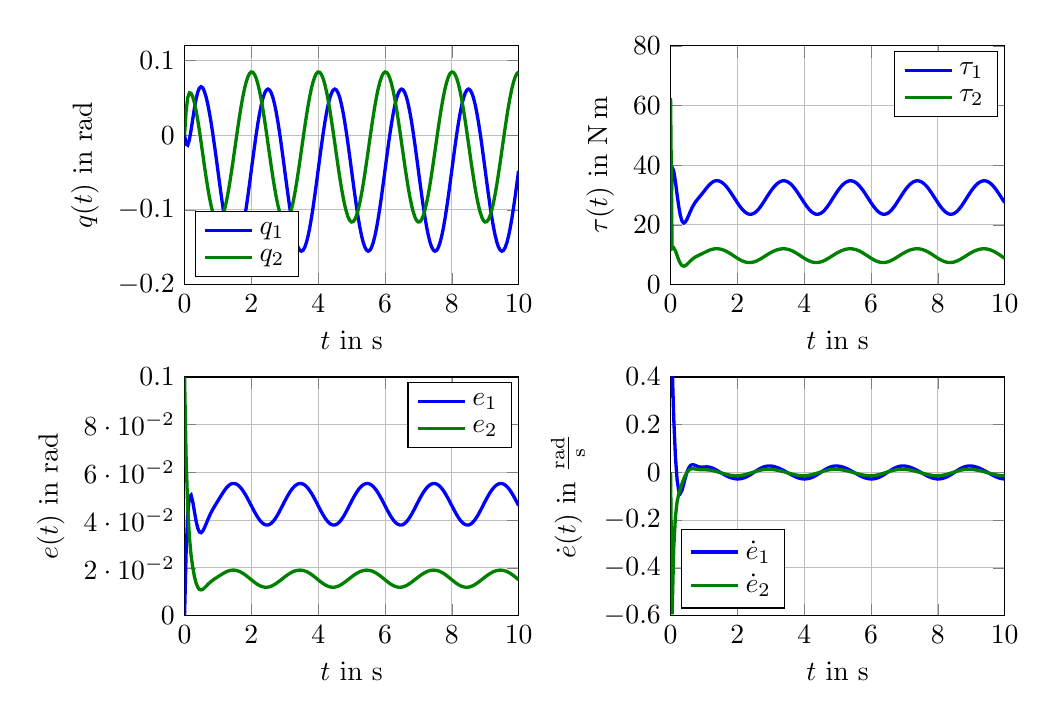
\begin{tikzpicture}

\begin{axis}[%
width=0.35\textwidth,
height=0.25\textwidth,
scale only axis,
xmin=0,
xmax=10,
xlabel={$t$ in $\mathrm{s}$},
xmajorgrids,
ymin=-0.2,
ymax=0.12,
ylabel={$q(t)$ in $\mathrm{rad}$},
ymajorgrids,
name=plot1,
legend style={at={(0.03,0.03)},anchor=south west,draw=black,fill=white,legend cell align=left}
]
\addplot [
color=blue,
solid,
line width=1.2pt
]
table[row sep=crcr]{
0 0\\
0.0455395182595911 -0.0117460746231492\\
0.0955395182595912 -0.0132236689560169\\
0.145539518259591 -0.00565329276728305\\
0.195539518259591 0.00712665794075456\\
0.245539518259591 0.0219921490805025\\
0.295539518259591 0.0364869248046341\\
0.345539518259591 0.0488537549767069\\
0.395539518259591 0.0580175771043982\\
0.445539518259591 0.0634942010665574\\
0.495539518259592 0.0652462017705019\\
0.545539518259592 0.0635225898608572\\
0.595539518259592 0.0587149490558528\\
0.645539518259592 0.0512504745821542\\
0.695539518259592 0.0415287725374959\\
0.745539518259592 0.029898357738129\\
0.795539518259592 0.016662144564355\\
0.845539518259592 0.00209889776337053\\
0.895539518259592 -0.0135113028552113\\
0.945539518259592 -0.0298663424864553\\
0.995539518259592 -0.0466308941560494\\
1.04553951825959 -0.0634359164964478\\
1.09553951825958 -0.0798872574189286\\
1.14553951825958 -0.0955803118912466\\
1.19553951825957 -0.110117330437932\\
1.24553951825957 -0.123124450943022\\
1.29553951825956 -0.134266444786907\\
1.34553951825955 -0.143258174795391\\
1.39553951825955 -0.149872603476924\\
1.44553951825954 -0.153945737865136\\
1.49553951825954 -0.155379136962218\\
1.54553951825953 -0.154140601479556\\
1.59553951825953 -0.150263510952599\\
1.64553951825952 -0.143845067997249\\
1.69553951825952 -0.135043528204059\\
1.74553951825951 -0.12407437934504\\
1.7955395182595 -0.111205396566335\\
1.8455395182595 -0.0967505292032254\\
1.89553951825949 -0.0810626450783237\\
1.94553951825949 -0.0645252419943057\\
1.99553951825948 -0.0475433105974585\\
2.04553951825948 -0.0305335837892446\\
2.09553951825947 -0.0139144312726084\\
2.14553951825947 0.00190434220449241\\
2.19553951825946 0.0165315506823531\\
2.24553951825945 0.0296043070379694\\
2.29553951825945 0.0407971175866683\\
2.34553951825944 0.0498301855568873\\
2.39553951825944 0.0564767162333854\\
2.44553951825943 0.0605690123655698\\
2.49553951825943 0.0620031489831389\\
2.54553951825942 0.0607420300521945\\
2.59553951825942 0.0568166619495169\\
2.64553951825941 0.0503255337341999\\
2.69553951825941 0.0414320703196169\\
2.7455395182594 0.0303602156606546\\
2.79553951825939 0.0173882985654453\\
2.84553951825939 0.00284142098161145\\
2.89553951825938 -0.0129173247944306\\
2.94553951825938 -0.0294964667170122\\
2.99553951825937 -0.0464862446527997\\
3.04553951825937 -0.0634688632139369\\
3.09553951825936 -0.0800286342143352\\
3.14553951825936 -0.0957617946139139\\
3.19553951825935 -0.110285839469793\\
3.24553951825934 -0.123248249136607\\
3.29553951825934 -0.134334510376136\\
3.34553951825933 -0.143275332303897\\
3.39553951825933 -0.14985294523283\\
3.44553951825932 -0.153906351677843\\
3.49553951825932 -0.155335383344229\\
3.54553951825931 -0.154103414162989\\
3.59553951825931 -0.150238593111477\\
3.6455395182593 -0.143833493850745\\
3.6955395182593 -0.13504312940814\\
3.74553951825929 -0.124081343989494\\
3.79553951825928 -0.111215662750016\\
3.84553951825928 -0.0967607452141191\\
3.89553951825927 -0.0810706410154184\\
3.94553951825927 -0.0645300821725537\\
3.99553951825926 -0.0475450622478301\\
4.04553951825928 -0.0305329513568652\\
4.09553951825929 -0.0139123822528195\\
4.14553951825931 0.0019068764211251\\
4.19553951825933 0.0165338610996999\\
4.24553951825934 0.0296059803156132\\
4.29553951825936 0.0407980204652113\\
4.34553951825938 0.0498303951091018\\
4.39553951825939 0.0564764298897514\\
4.44553951825941 0.0605684639414358\\
4.49553951825943 0.0620025463858268\\
4.54553951825944 0.0607415202341098\\
4.59553951825946 0.0568163209767773\\
4.64553951825948 0.050325375308299\\
4.69553951825949 0.0414320645404638\\
4.74553951825951 0.0303603105218574\\
4.79553951825953 0.0173884386954534\\
4.84553951825954 0.00284156061395274\\
4.89553951825956 -0.0129172153846358\\
4.94553951825958 -0.0294964004282345\\
4.99553951825959 -0.0464862206431125\\
5.04553951825961 -0.0634688718617205\\
5.09553951825963 -0.0800286622415356\\
5.14553951825964 -0.0957618292141662\\
5.19553951825966 -0.110285870897851\\
5.24553951825968 -0.123248271736022\\
5.29553951825969 -0.134334522367753\\
5.34553951825971 -0.143275334813342\\
5.39553951825973 -0.149852941032645\\
5.44553951825974 -0.15390634401513\\
5.49553951825976 -0.155335375076286\\
5.54553951825978 -0.154103407279107\\
5.59553951825979 -0.150238588608573\\
5.64553951825981 -0.143833491865802\\
5.69553951825983 -0.13504312948921\\
5.74553951825984 -0.124081345398613\\
5.79553951825986 -0.111215664721745\\
5.84553951825988 -0.0967607471296271\\
5.89553951825989 -0.0810706424841412\\
5.94553951825991 -0.0645300830361876\\
5.99553951825993 -0.0475450625329911\\
6.04553951825995 -0.0305329512046135\\
6.09553951825996 -0.0139123818483474\\
6.14553951825998 0.00190687690357465\\
6.19553951826 0.0165338615302122\\
6.24553951826001 0.0296059806207711\\
6.29553951826003 0.0407980206239322\\
6.34553951826005 0.049830395138792\\
6.39553951826006 0.0564764298291398\\
6.44553951826008 0.0605684638349004\\
6.4955395182601 0.0620025462720104\\
6.54553951826011 0.0607415201397269\\
6.59553951826013 0.056816320915104\\
6.64553951826015 0.0503253752810316\\
6.69553951826016 0.0414320645413836\\
6.74553951826018 0.0303603105409013\\
6.7955395182602 0.0173884387221911\\
6.84553951826021 0.002841560639938\\
6.89553951826023 -0.0129172153647492\\
6.94553951826025 -0.0294964004166255\\
6.99553951826026 -0.0464862206394256\\
7.04553951826028 -0.0634688718640228\\
7.0955395182603 -0.0800286622472797\\
7.14553951826031 -0.0957618292209513\\
7.19553951826033 -0.110285870903887\\
7.24553951826035 -0.123248271740299\\
7.29553951826036 -0.134334522369989\\
7.34553951826038 -0.143275334813785\\
7.3955395182604 -0.149852941031835\\
7.44553951826041 -0.153906344013681\\
7.49553951826043 -0.155335375074728\\
7.54553951826045 -0.154103407277801\\
7.59553951826046 -0.150238588607693\\
7.64553951826048 -0.143833491865363\\
7.6955395182605 -0.135043129489122\\
7.74553951826051 -0.124081345398736\\
7.79553951826053 -0.11121566472194\\
7.84553951826055 -0.0967607471297835\\
7.89553951826056 -0.0810706424841944\\
7.94553951826058 -0.0645300830361163\\
7.9955395182606 -0.0475450625328085\\
8.04553951826057 -0.0305329512043543\\
8.09553951826054 -0.013912381848056\\
8.14553951826052 0.00190687690385699\\
8.19553951826049 0.0165338615304546\\
8.24553951826046 0.0296059806209562\\
8.29553951826043 0.0407980206240551\\
8.34553951826041 0.0498303951388575\\
8.39553951826038 0.0564764298291587\\
8.44553951826035 0.0605684638348858\\
8.49553951826032 0.0620025462719752\\
8.54553951826029 0.060741520139682\\
8.59553951826027 0.0568163209150578\\
8.64553951826024 0.05032537528099\\
8.69553951826021 0.0414320645413504\\
8.74553951826018 0.0303603105408792\\
8.79553951826016 0.0173884387221818\\
8.84553951826013 0.002841560639943\\
8.8955395182601 -0.012917215364729\\
8.94553951826007 -0.0294964004165896\\
8.99553951826005 -0.0464862206393739\\
9.04553951826002 -0.0634688718639562\\
9.09553951825999 -0.0800286622472002\\
9.14553951825996 -0.0957618292208617\\
9.19553951825993 -0.110285870903791\\
9.24553951825991 -0.123248271740203\\
9.29553951825988 -0.134334522369897\\
9.34553951825985 -0.143275334813704\\
9.39553951825982 -0.149852941031771\\
9.4455395182598 -0.15390634401364\\
9.49553951825977 -0.155335375074715\\
9.54553951825974 -0.154103407277822\\
9.59553951825971 -0.150238588607752\\
9.64553951825969 -0.143833491865463\\
9.69553951825966 -0.135043129489266\\
9.74553951825963 -0.124081345398923\\
9.7955395182596 -0.111215664722169\\
9.84553951825957 -0.096760747130052\\
9.89553951825955 -0.0810706424844977\\
9.94553951825952 -0.0645300830364486\\
9.99553951825949 -0.0475450625331623\\
};
\addlegendentry{$q_1$};

\addplot [
color=green!50!black,
solid,
line width=1.2pt
]
table[row sep=crcr]{
0 0\\
0.0455395182595911 0.0323744658510274\\
0.0955395182595912 0.0507319891351314\\
0.145539518259591 0.0569633386662316\\
0.195539518259591 0.0564055089888706\\
0.245539518259591 0.0515493461379264\\
0.295539518259591 0.0435401767031275\\
0.345539518259591 0.0329772188620955\\
0.395539518259591 0.020311421007536\\
0.445539518259591 0.00601327602377142\\
0.495539518259592 -0.00938539800805047\\
0.545539518259592 -0.0253106161658608\\
0.595539518259592 -0.0411862912466375\\
0.645539518259592 -0.056472695625054\\
0.695539518259592 -0.070693154087518\\
0.745539518259592 -0.0834469096644321\\
0.795539518259592 -0.0944106854658524\\
0.845539518259592 -0.103333318215173\\
0.895539518259592 -0.110027820056058\\
0.945539518259592 -0.114364138049934\\
0.995539518259592 -0.116264393958552\\
1.04553951825959 -0.115700986912302\\
1.09553951825958 -0.112696917139974\\
1.14553951825958 -0.107327145745699\\
1.19553951825957 -0.0997197076987002\\
1.24553951825957 -0.090055521472544\\
1.29553951825956 -0.0785662376493497\\
1.34553951825955 -0.0655299014131569\\
1.39553951825955 -0.0512645695781131\\
1.44553951825954 -0.0361202683866121\\
1.49553951825954 -0.0204697940172956\\
1.54553951825953 -0.00469886520959869\\
1.59553951825953 0.0108039256002417\\
1.64553951825952 0.0256570099438129\\
1.69553951825952 0.0394953296311976\\
1.74553951825951 0.0519792236607736\\
1.7955395182595 0.0628025727854834\\
1.8455395182595 0.071700079992937\\
1.89553951825949 0.0784535709874601\\
1.94553951825949 0.082897199167472\\
1.99553951825948 0.0849214429712913\\
2.04553951825948 0.0844757950827712\\
2.09553951825947 0.0815700646207297\\
2.14553951825947 0.076274243920914\\
2.19553951825946 0.0687169278134342\\
2.24553951825945 0.0590823116766924\\
2.29553951825945 0.0476058316545703\\
2.34553951825944 0.0345685439836292\\
2.39553951825944 0.0202903694859277\\
2.44553951825943 0.00512235426853042\\
2.49553951825943 -0.0105618803664477\\
2.54553951825942 -0.0263753056149734\\
2.59553951825942 -0.0419270581197639\\
2.64553951825941 -0.0568321878660948\\
2.69553951825941 -0.0707213352472953\\
2.7455395182594 -0.0832500807943158\\
2.79553951825939 -0.09410770783798\\
2.84553951825939 -0.103025125286809\\
2.89553951825938 -0.109781716592288\\
2.94553951825938 -0.114210912307357\\
2.99553951825937 -0.116204326224598\\
3.04553951825937 -0.115714346083716\\
3.09553951825936 -0.112755125213079\\
3.14553951825936 -0.107401976627555\\
3.19553951825935 -0.0997892217363705\\
3.24553951825934 -0.0901065886550973\\
3.29553951825934 -0.0785942884546642\\
3.34553951825933 -0.0655369215017693\\
3.39553951825933 -0.0512563817760474\\
3.44553951825932 -0.0361039370060312\\
3.49553951825932 -0.0204516691644777\\
3.54553951825931 -0.00468346537899601\\
3.59553951825931 0.0108142451657239\\
3.6455395182593 0.0256618071054086\\
3.6955395182593 0.0394955013804173\\
3.74553951825929 0.0519763454264541\\
3.79553951825928 0.0627983234339268\\
3.84553951825928 0.0716958459110578\\
3.89553951825927 0.0784502513926428\\
3.94553951825927 0.0828951838729425\\
3.99553951825926 0.0849207069834184\\
4.04553951825928 0.0844760488840701\\
4.09553951825929 0.081570908485525\\
4.14553951825931 0.0762752918290922\\
4.19553951825933 0.0687178850894306\\
4.24553951825934 0.0590830059458408\\
4.29553951825936 0.047606206846646\\
4.34553951825938 0.034568631612482\\
4.39553951825939 0.0202902513038148\\
4.44553951825941 0.00512212728767294\\
4.49553951825943 -0.010562129859458\\
4.54553951825944 -0.0263755166716259\\
4.59553951825946 -0.0419271992456766\\
4.64553951825948 -0.0568322534399539\\
4.69553951825949 -0.0707213376932001\\
4.74553951825951 -0.0832500416496824\\
4.79553951825953 -0.0941076499953191\\
4.84553951825954 -0.103025067645769\\
4.89553951825956 -0.109781671419338\\
4.94553951825958 -0.114210884924888\\
4.99553951825959 -0.116204316288909\\
5.04553951825961 -0.115714349629926\\
5.09553951825963 -0.11275513676527\\
5.14553951825964 -0.107401990900213\\
5.19553951825966 -0.0997892347038503\\
5.24553951825968 -0.0901065979783353\\
5.29553951825969 -0.0785942933963273\\
5.34553951825971 -0.0655369225259095\\
5.39553951825973 -0.0512563800284846\\
5.44553951825974 -0.0361039338292461\\
5.49553951825976 -0.0204516657397162\\
5.54553951825978 -0.00468346252835103\\
5.59553951825979 0.0108142470305807\\
5.64553951825981 0.0256618079282011\\
5.69553951825983 0.0394955013480815\\
5.74553951825984 0.0519763448439852\\
5.79553951825986 0.062798322617704\\
5.84553951825988 0.0716958451170669\\
5.89553951825989 0.0784502507827597\\
5.94553951825991 0.0828951835131702\\
5.99553951825993 0.0849207068632647\\
6.04553951825995 0.0844760489455198\\
6.09553951825996 0.081570908652047\\
6.14553951825998 0.0762752920284594\\
6.19553951826 0.0687178852676395\\
6.24553951826001 0.0590830060722664\\
6.29553951826003 0.0476062069124005\\
6.34553951826005 0.0345686316247085\\
6.39553951826006 0.0202902512785594\\
6.44553951826008 0.00512212724335558\\
6.4955395182601 -0.0105621299067938\\
6.54553951826011 -0.0263755167108952\\
6.59553951826013 -0.0419271992713783\\
6.64553951826015 -0.0568322534513912\\
6.69553951826016 -0.0707213376929521\\
6.74553951826018 -0.083250041641913\\
6.7955395182602 -0.0941076499843381\\
6.84553951826021 -0.103025067635063\\
6.89553951826023 -0.109781671411112\\
6.94553951826025 -0.114210884920042\\
6.99553951826026 -0.116204316287298\\
7.04553951826028 -0.115714349630756\\
7.0955395182603 -0.112755136767493\\
7.14553951826031 -0.107401990902842\\
7.19553951826033 -0.0997892347061485\\
7.24553951826035 -0.0901065979798913\\
7.29553951826036 -0.0785942933970285\\
7.34553951826038 -0.0655369225258638\\
7.3955395182604 -0.0512563800279208\\
7.44553951826041 -0.0361039338284238\\
7.49553951826043 -0.0204516657388597\\
7.54553951826045 -0.00468346252761468\\
7.59553951826046 0.0108142470311202\\
7.64553951826048 0.0256618079285332\\
7.6955395182605 0.0394955013482399\\
7.74553951826051 0.0519763448440244\\
7.79553951826053 0.0627983226176798\\
7.84553951826055 0.0716958451170232\\
7.89553951826056 0.0784502507827229\\
7.94553951826058 0.0828951835131495\\
7.9955395182606 0.0849207068632561\\
8.04553951826057 0.0844760489455131\\
8.09553951826054 0.0815709086520316\\
8.14553951826052 0.0762752920284257\\
8.19553951826049 0.0687178852675817\\
8.24553951826046 0.0590830060721838\\
8.29553951826043 0.047606206912297\\
8.34553951826041 0.0345686316245911\\
8.39553951826038 0.0202902512784366\\
8.44553951826035 0.00512212724323568\\
8.49553951826032 -0.0105621299069036\\
8.54553951826029 -0.0263755167109898\\
8.59553951826027 -0.0419271992714548\\
8.64553951826024 -0.0568322534514487\\
8.69553951826021 -0.0707213376929915\\
8.74553951826018 -0.0832500416419368\\
8.79553951826016 -0.0941076499843494\\
8.84553951826013 -0.103025067635066\\
8.8955395182601 -0.10978167141111\\
8.94553951826007 -0.11421088492004\\
8.99553951826005 -0.116204316287301\\
9.04553951826002 -0.115714349630767\\
9.09553951825999 -0.112755136767516\\
9.14553951825996 -0.10740199090288\\
9.19553951825993 -0.0997892347062061\\
9.24553951825991 -0.0901065979799697\\
9.29553951825988 -0.078594293397129\\
9.34553951825985 -0.0655369225259867\\
9.39553951825982 -0.0512563800280654\\
9.4455395182598 -0.036103933828588\\
9.49553951825977 -0.0204516657390404\\
9.54553951825974 -0.00468346252780774\\
9.59553951825971 0.01081424703092\\
9.64553951825969 0.0256618079283319\\
9.69553951825966 0.0394955013480443\\
9.74553951825963 0.0519763448438417\\
9.7955395182596 0.0627983226175174\\
9.84553951825957 0.0716958451168885\\
9.89553951825955 0.0784502507826231\\
9.94553951825952 0.0828951835130911\\
9.99553951825949 0.0849207068632448\\
};
\addlegendentry{$q_2$};

\end{axis}

\begin{axis}[%
width=0.35\textwidth,
height=0.25\textwidth,
scale only axis,
xmin=0,
xmax=10,
xlabel={$t$ in $\mathrm{s}$},
xmajorgrids,
ymin=0,
ymax=0.1,
ylabel={$e(t)$ in $\mathrm{rad}$},
ymajorgrids,
name=plot3,
at=(plot1.below south west),
anchor=above north west,
legend style={draw=black,fill=white,legend cell align=left}
]
\addplot [
color=blue,
solid,
line width=1.2pt
]
table[row sep=crcr]{
0 0\\
0.0455395182595911 0.0260039812205406\\
0.0955395182595912 0.0427896609772418\\
0.145539518259591 0.0497993573648771\\
0.195539518259591 0.0505124566104274\\
0.245539518259591 0.0477207491307633\\
0.295539518259591 0.0435831941489097\\
0.345539518259591 0.0396019926529892\\
0.395539518259591 0.0366457251270117\\
0.445539518259591 0.035045731096141\\
0.495539518259592 0.0347439801583542\\
0.545539518259592 0.0354557517066799\\
0.595539518259592 0.0368143768906902\\
0.645539518259592 0.0384775866949348\\
0.695539518259592 0.0401886214111349\\
0.745539518259592 0.0417962154385465\\
0.795539518259592 0.0432442495081089\\
0.845539518259592 0.0445442229648944\\
0.895539518259592 0.0457426418073047\\
0.945539518259592 0.0468922571276955\\
0.995539518259592 0.0480321499621981\\
1.04553951825959 0.0491780098990576\\
1.09553951825958 0.0503212653977066\\
1.14553951825958 0.0514342472936569\\
1.19553951825957 0.0524782158867556\\
1.24553951825957 0.0534115527317623\\
1.29553951825956 0.0541963258333688\\
1.34553951825955 0.0548024271657008\\
1.39553951825955 0.0552093012455189\\
1.44553951825954 0.0554058057024403\\
1.49553951825954 0.0553889550333622\\
1.54553951825953 0.0551622599120163\\
1.59553951825953 0.0547341850060501\\
1.64553951825952 0.0541170067201505\\
1.69553951825952 0.0533261342554149\\
1.74553951825951 0.0523798061683466\\
1.7955395182595 0.0512990024938496\\
1.8455395182595 0.0501074084749346\\
1.89553951825949 0.0488313061262009\\
1.94553951825949 0.0474993273530332\\
1.99553951825948 0.0461420547912753\\
2.04553951825948 0.0447914903866005\\
2.09553951825947 0.0434804232937973\\
2.14553951825947 0.0422417223930663\\
2.19553951825946 0.0411075638687952\\
2.24553951825945 0.0401085911732657\\
2.29553951825945 0.0392730013668488\\
2.34553951825944 0.0386255620727872\\
2.39553951825944 0.038186585998009\\
2.44553951825943 0.03797091979712\\
2.49553951825943 0.0379870329457165\\
2.54553951825942 0.0382363115153503\\
2.59553951825942 0.0387126639970425\\
2.64553951825941 0.0394025275429142\\
2.69553951825941 0.0402853236290476\\
2.7455395182594 0.041334357516063\\
2.79553951825939 0.0425180955070683\\
2.84553951825939 0.0438016997467099\\
2.89553951825938 0.0451486637465861\\
2.94553951825938 0.0465223813583188\\
2.99553951825937 0.0478875004590175\\
3.04553951825937 0.0492109566166153\\
3.09553951825936 0.0504626421931794\\
3.14553951825936 0.0516157300163862\\
3.19553951825935 0.0526467249186731\\
3.24553951825934 0.0535353509253971\\
3.29553951825934 0.0542643914226401\\
3.34553951825933 0.0548195846742383\\
3.39553951825933 0.0551896430014463\\
3.44553951825932 0.0553664195151593\\
3.49553951825932 0.055345201415374\\
3.54553951825931 0.055125072595439\\
3.59553951825931 0.0547092671649072\\
3.6455395182593 0.0541054325736154\\
3.6955395182593 0.0533257354594554\\
3.74553951825929 0.0523867708127528\\
3.79553951825928 0.051309268677475\\
3.84553951825928 0.050117624485767\\
3.89553951825927 0.0488393020632301\\
3.94553951825927 0.047504167531213\\
3.99553951825926 0.0461438064415778\\
4.04553951825928 0.044790857954159\\
4.09553951825929 0.0434783742739552\\
4.14553951825931 0.0422391881763898\\
4.19553951825933 0.0411052534514142\\
4.24553951825934 0.0401069178955969\\
4.29553951825936 0.0392720984882891\\
4.34553951825938 0.038625352520563\\
4.39553951825939 0.0381868723416385\\
4.44553951825941 0.0379714682212529\\
4.49553951825943 0.0379876355430285\\
4.54553951825944 0.038236821333434\\
4.59553951825946 0.0387130049697779\\
4.64553951825948 0.0394026859688059\\
4.69553951825949 0.0402853294081847\\
4.74553951825951 0.0413342626548358\\
4.79553951825953 0.0425179553770266\\
4.84553951825954 0.0438015601143255\\
4.89553951825956 0.0451485543367385\\
4.94553951825958 0.0465223150694793\\
4.99553951825959 0.0478874764492605\\
5.04553951825961 0.049210965264323\\
5.09553951825963 0.0504626702202996\\
5.14553951825964 0.0516157646165573\\
5.19553951825966 0.0526467563466513\\
5.24553951825968 0.0535353735247364\\
5.29553951825969 0.05426440341419\\
5.34553951825971 0.0548195871836287\\
5.39553951825973 0.0551896388012216\\
5.44553951825974 0.0553664118524236\\
5.49553951825976 0.0553451931474294\\
5.54553951825978 0.0551250657115784\\
5.59553951825979 0.054709262662049\\
5.64553951825981 0.054105430588743\\
5.69553951825983 0.0533257355406225\\
5.74553951825984 0.0523867722219923\\
5.79553951825986 0.0513092706493491\\
5.84553951825988 0.0501176264014415\\
5.89553951825989 0.0488393035321378\\
5.94553951825991 0.0475041683950461\\
5.99553951825993 0.046143806726948\\
6.04553951825995 0.0447908578021147\\
6.09553951825996 0.0434783738696834\\
6.14553951825998 0.0422391876941283\\
6.19553951826 0.0411052530210734\\
6.24553951826001 0.0401069175905893\\
6.29553951826003 0.0392720983296939\\
6.34553951826005 0.0386253524909705\\
6.39553951826006 0.0381868724023178\\
6.44553951826008 0.0379714683278241\\
6.4955395182601 0.0379876356568479\\
6.54553951826011 0.038236821427787\\
6.59553951826013 0.0387130050313891\\
6.64553951826015 0.0394026859959806\\
6.69553951826016 0.0402853294071439\\
6.74553951826018 0.0413342626356456\\
6.7955395182602 0.042517955350121\\
6.84553951826021 0.0438015600881545\\
6.89553951826023 0.0451485543166534\\
6.94553951826025 0.0465223150576634\\
6.99553951826026 0.0478874764453639\\
7.04553951826028 0.0492109652664175\\
7.0955395182603 0.0504626702258435\\
7.14553951826031 0.0516157646231539\\
7.19553951826033 0.0526467563525156\\
7.24553951826035 0.0535353735288635\\
7.29553951826036 0.0542644034163006\\
7.34553951826038 0.0548195871839736\\
7.3955395182604 0.0551896388003441\\
7.44553951826041 0.055366411850939\\
7.49553951826043 0.0553451931458684\\
7.54553951826045 0.0551250657103021\\
7.59553951826046 0.0547092626612306\\
7.64553951826048 0.0541054305883967\\
7.6955395182605 0.053325735540655\\
7.74553951826051 0.0523867722222619\\
7.79553951826053 0.0513092706497116\\
7.84553951826055 0.0501176264017837\\
7.89553951826056 0.0488393035323894\\
7.94553951826058 0.0475041683951817\\
7.9955395182606 0.046143806726975\\
8.04553951826057 0.0447908578020506\\
8.09553951826054 0.0434783738695668\\
8.14553951826052 0.0422391876939977\\
8.19553951826049 0.0411052530209578\\
8.24553951826046 0.0401069175905055\\
8.29553951826043 0.0392720983296471\\
8.34553951826041 0.0386253524909578\\
8.39553951826038 0.0381868724023309\\
8.44553951826035 0.0379714683278531\\
8.49553951826032 0.037987635656884\\
8.54553951826029 0.0382368214278237\\
8.59553951826027 0.0387130050314224\\
8.64553951826024 0.0394026859960092\\
8.69553951826021 0.0402853294071681\\
8.74553951826018 0.0413342626356667\\
8.79553951826016 0.04251795535014\\
8.84553951826013 0.0438015600881728\\
8.8955395182601 0.0451485543166712\\
8.94553951826007 0.0465223150576811\\
8.99553951826005 0.0478874764453801\\
9.04553951826002 0.0492109652664322\\
9.09553951825999 0.0504626702258557\\
9.14553951825996 0.0516157646231633\\
9.19553951825993 0.0526467563525211\\
9.24553951825991 0.0535353735288657\\
9.29553951825988 0.0542644034162993\\
9.34553951825985 0.0548195871839695\\
9.39553951825982 0.0551896388003374\\
9.4455395182598 0.0553664118509305\\
9.49553951825977 0.0553451931458586\\
9.54553951825974 0.0551250657102918\\
9.59553951825971 0.0547092626612206\\
9.64553951825969 0.0541054305883873\\
9.69553951825966 0.0533257355406471\\
9.74553951825963 0.0523867722222555\\
9.7955395182596 0.0513092706497075\\
9.84553951825957 0.0501176264017822\\
9.89553951825955 0.0488393035323907\\
9.94553951825952 0.0475041683951856\\
9.99553951825949 0.0461438067269817\\
};
\addlegendentry{$e_1$};

\addplot [
color=green!50!black,
solid,
line width=1.2pt
]
table[row sep=crcr]{
0 0.1\\
0.0455395182595911 0.0666038757165098\\
0.0955395182595912 0.0447973368114116\\
0.145539518259591 0.0327647226108575\\
0.195539518259591 0.0253118849597603\\
0.245539518259591 0.0201452270387493\\
0.295539518259591 0.0163662173693365\\
0.345539518259591 0.0136659018661696\\
0.395539518259591 0.0119199179445576\\
0.445539518259591 0.011012638617469\\
0.495539518259592 0.0107866538141993\\
0.545539518259592 0.0110527095684693\\
0.595539518259592 0.0116202992254124\\
0.645539518259592 0.0123266310274598\\
0.695539518259592 0.013054039536336\\
0.745539518259592 0.0137340114531662\\
0.795539518259592 0.0143405665123085\\
0.845539518259592 0.0148775705854772\\
0.895539518259592 0.0153645178246485\\
0.945539518259592 0.015824205887236\\
0.995539518259592 0.0162742120296962\\
1.04553951825959 0.0167226453447643\\
1.09553951825958 0.0171675911934299\\
1.14553951825958 0.0175990844686082\\
1.19553951825957 0.0180023137500656\\
1.24553951825957 0.0183609482958626\\
1.29553951825956 0.0186598435768777\\
1.34553951825955 0.0188867806848815\\
1.39553951825955 0.0190332306260067\\
1.44553951825954 0.0190943537453567\\
1.49553951825954 0.0190685382111298\\
1.54553951825953 0.0189567718069717\\
1.59553951825953 0.0187620664209637\\
1.64553951825952 0.0184890546537613\\
1.69553951825952 0.0181437849199648\\
1.74553951825951 0.0177336745504738\\
1.7955395182595 0.017267546168044\\
1.8455395182595 0.0167556676367456\\
1.89553951825949 0.0162097312439399\\
1.94553951825949 0.0156427329952208\\
1.99553951825948 0.0150687389575643\\
2.04553951825948 0.0145025464847711\\
2.09553951825947 0.0139592613258245\\
2.14553951825947 0.0134538173561925\\
2.19553951825946 0.0130004661352204\\
2.24553951825945 0.0126122615000132\\
2.29553951825945 0.0123005624179294\\
2.34553951825944 0.0120745767446769\\
2.39553951825944 0.0119409694662114\\
2.44553951825943 0.0119035603727591\\
2.49553951825943 0.0119631361726481\\
2.54553951825942 0.0121173990176347\\
2.59553951825942 0.0123610660985916\\
2.64553951825941 0.0126861232685517\\
2.69553951825941 0.0130822206961612\\
2.7455395182594 0.0135371825830931\\
2.79553951825939 0.0140375888844733\\
2.84553951825939 0.0145693776571421\\
2.89553951825938 0.015118414360899\\
2.94553951825938 0.0156709801446698\\
2.99553951825937 0.0162141442957433\\
3.04553951825937 0.0167360045161683\\
3.09553951825936 0.0172257992665142\\
3.14553951825936 0.017673915350433\\
3.19553951825935 0.0180718277876959\\
3.24553951825934 0.0184120154783676\\
3.29553951825934 0.0186878943821368\\
3.34553951825933 0.0188938007734327\\
3.39553951825933 0.0190250428238756\\
3.44553951825932 0.0190780223647075\\
3.49553951825932 0.0190504133582426\\
3.54553951825931 0.0189413719763005\\
3.59553951825931 0.0187517468554155\\
3.6455395182593 0.0184842574921034\\
3.6955395182593 0.0181436131706885\\
3.74553951825929 0.0177365527847438\\
3.79553951825928 0.0172717955195592\\
3.84553951825928 0.0167599017185924\\
3.89553951825927 0.0162130508387349\\
3.94553951825927 0.0156447482897385\\
3.99553951825926 0.0150694749454362\\
4.04553951825928 0.0145022926834812\\
4.09553951825929 0.0139584174610457\\
4.14553951825931 0.0134527694480358\\
4.19553951825933 0.0129995088592481\\
4.24553951825934 0.012611567230889\\
4.29553951825936 0.012300187225876\\
4.34553951825938 0.0120744891158426\\
4.39553951825939 0.0119410876483375\\
4.44553951825941 0.0119037873536235\\
4.49553951825943 0.0119633856656584\\
4.54553951825944 0.0121176100742803\\
4.59553951825946 0.0123612072244909\\
4.64553951825948 0.012686188842392\\
4.69553951825949 0.0130822231420432\\
4.74553951825951 0.0135371434384348\\
4.79553951825953 0.0140375310417874\\
4.84553951825954 0.0145693200160802\\
4.89553951825956 0.0151183691879311\\
4.94553951825958 0.01567095276219\\
4.99553951825959 0.0162141343600528\\
5.04553951825961 0.0167360080623898\\
5.09553951825963 0.0172258108187305\\
5.14553951825964 0.0176739296231316\\
5.19553951825966 0.0180718407552321\\
5.24553951825968 0.0184120248016786\\
5.29553951825969 0.0186878993238893\\
5.34553951825971 0.0188938017976776\\
5.39553951825973 0.0190250410764316\\
5.44553951825974 0.0190780191880529\\
5.49553951825976 0.0190504099336208\\
5.54553951825978 0.0189413691258004\\
5.59553951825979 0.0187517449907054\\
5.64553951825981 0.0184842566694548\\
5.69553951825983 0.0181436132031612\\
5.74553951825984 0.0177365533673376\\
5.79553951825986 0.0172717963358907\\
5.84553951825988 0.0167599025126712\\
5.89553951825989 0.016213051448681\\
5.94553951825991 0.0156447486495453\\
5.99553951825993 0.0150694750655929\\
6.04553951825995 0.0145022926220015\\
6.09553951825996 0.0139584172944617\\
6.14553951825998 0.0134527692485761\\
6.19553951826 0.0129995086809183\\
6.24553951826001 0.0126115671043173\\
6.29553951826003 0.0123001871599535\\
6.34553951826005 0.0120744891034307\\
6.39553951826006 0.0119410876733943\\
6.44553951826008 0.011903787397734\\
6.4955395182601 0.0119633857127845\\
6.54553951826011 0.0121176101133418\\
6.59553951826013 0.0123612072499922\\
6.64553951826015 0.0126861888536409\\
6.69553951826016 0.0130822231416237\\
6.74553951826018 0.0135371434305149\\
6.7955395182602 0.0140375310306807\\
6.84553951826021 0.014569320005276\\
6.89553951826023 0.0151183691796377\\
6.94553951826025 0.0156709527573083\\
6.99553951826026 0.0162141343584392\\
7.04553951826028 0.0167360080632495\\
7.0955395182603 0.0172258108210152\\
7.14553951826031 0.0176739296258525\\
7.19553951826033 0.0180718407576511\\
7.24553951826035 0.0184120248033809\\
7.29553951826036 0.0186878993247583\\
7.34553951826038 0.0188938017978176\\
7.3955395182604 0.0190250410760663\\
7.44553951826041 0.0190780191874375\\
7.49553951826043 0.0190504099329738\\
7.54553951826045 0.0189413691252718\\
7.59553951826046 0.0187517449903661\\
7.64553951826048 0.0184842566693112\\
7.6955395182605 0.0181436132031741\\
7.74553951826051 0.0177365533674489\\
7.79553951826053 0.0172717963360404\\
7.84553951826055 0.0167599025128128\\
7.89553951826056 0.0162130514487853\\
7.94553951826058 0.0156447486496017\\
7.9955395182606 0.0150694750656044\\
8.04553951826057 0.0145022926219801\\
8.09553951826054 0.013958417294423\\
8.14553951826052 0.0134527692485352\\
8.19553951826049 0.0129995086808866\\
8.24553951826046 0.0126115671043013\\
8.29553951826043 0.0123001871599552\\
8.34553951826041 0.0120744891034479\\
8.39553951826038 0.011941087673423\\
8.44553951826035 0.0119037873977699\\
8.49553951826032 0.0119633857128229\\
8.54553951826029 0.0121176101133798\\
8.59553951826027 0.012361207250027\\
8.64553951826024 0.012686188853672\\
8.69553951826021 0.0130822231416504\\
8.74553951826018 0.0135371434305376\\
8.79553951826016 0.0140375310306992\\
8.84553951826013 0.014569320005291\\
8.8955395182601 0.0151183691796489\\
8.94553951826007 0.0156709527573158\\
8.99553951826005 0.0162141343584425\\
9.04553951826002 0.0167360080632486\\
9.09553951825999 0.0172258108210099\\
9.14553951825996 0.0176739296258428\\
9.19553951825993 0.0180718407576374\\
9.24553951825991 0.0184120248033632\\
9.29553951825988 0.0186878993247374\\
9.34553951825985 0.0188938017977938\\
9.39553951825982 0.019025041076041\\
9.4455395182598 0.0190780191874109\\
9.49553951825977 0.0190504099329471\\
9.54553951825974 0.0189413691252454\\
9.59553951825971 0.0187517449903412\\
9.64553951825969 0.0184842566692886\\
9.69553951825966 0.0181436132031546\\
9.74553951825963 0.0177365533674326\\
9.7955395182596 0.0172717963360283\\
9.84553951825957 0.0167599025128052\\
9.89553951825955 0.0162130514487823\\
9.94553951825952 0.0156447486496033\\
9.99553951825949 0.0150694750656108\\
};
\addlegendentry{$e_2$};

\end{axis}

\begin{axis}[%
width=0.35\textwidth,
height=0.25\textwidth,
scale only axis,
xmin=0,
xmax=10,
xlabel={$t$ in $\mathrm{s}$},
xmajorgrids,
ymin=-0.6,
ymax=0.4,
ylabel={$\dot{e}(t)$ in $\mathrm{\frac{rad}{s}}$},
ymajorgrids,
name=plot2,
at=(plot3.right of south east),
anchor=left of south west,
legend style={at={(0.03,0.03)},anchor=south west,draw=black,fill=white,legend cell align=left}
]
\addplot [
color=blue,
solid,
line width=1.2pt
]
table[row sep=crcr]{
0 0.314159265358979\\
0.0455395182595911 0.461054352494977\\
0.0955395182595912 0.224352520335091\\
0.145539518259591 0.0659360482796881\\
0.195539518259591 -0.030284594134737\\
0.245539518259591 -0.0768892360724568\\
0.295539518259591 -0.0868026869312594\\
0.345539518259591 -0.073169938531883\\
0.395539518259591 -0.0479218049785774\\
0.445539518259591 -0.0204335829784504\\
0.495539518259592 0.00314799704165468\\
0.545539518259592 0.0198405675952214\\
0.595539518259592 0.029216040517185\\
0.645539518259592 0.0325215905282742\\
0.695539518259592 0.031786220590741\\
0.745539518259592 0.0290915718273809\\
0.795539518259592 0.0260955331643598\\
0.845539518259592 0.0238176873087723\\
0.895539518259592 0.0226397847886193\\
0.945539518259592 0.0224461181386309\\
0.995539518259592 0.0228249751836908\\
1.04553951825959 0.0232662725468196\\
1.09553951825958 0.0233135016295933\\
1.14553951825958 0.0226524504961979\\
1.19553951825957 0.0211391267159786\\
1.24553951825957 0.018781953771437\\
1.29553951825956 0.0156982578561725\\
1.34553951825955 0.0120637767951936\\
1.39553951825955 0.00806882480834237\\
1.44553951825954 0.00388832561244103\\
1.49553951825954 -0.000332870572209421\\
1.54553951825953 -0.00448201859194082\\
1.59553951825953 -0.00847246998856514\\
1.64553951825952 -0.0122344211501409\\
1.69553951825952 -0.0157061990010019\\
1.74553951825951 -0.0188283119441903\\
1.7955395182595 -0.0215409603702462\\
1.8455395182595 -0.0237845519019212\\
1.89553951825949 -0.025502155291186\\
1.94553951825949 -0.0266427282920469\\
1.99553951825948 -0.0271642239358243\\
2.04553951825948 -0.0270361195544248\\
2.09553951825947 -0.0262413363666218\\
2.14553951825947 -0.0247777911197993\\
2.19553951825946 -0.0226598870002835\\
2.24553951825945 -0.01992012413739\\
2.29553951825945 -0.0166107603313751\\
2.34553951825944 -0.012805176566765\\
2.39553951825944 -0.00859839451517209\\
2.44553951825943 -0.00410612622882734\\
2.49553951825943 0.000538155850517357\\
2.54553951825942 0.00518836534852704\\
2.59553951825942 0.00969300748075333\\
2.64553951825941 0.0139038529405489\\
2.69553951825941 0.017685114295589\\
2.7455395182594 0.0209219365569685\\
2.79553951825939 0.0235270127043563\\
2.84553951825939 0.0254443783288068\\
2.89553951825938 0.0266498919447686\\
2.94553951825938 0.0271484789776982\\
2.99553951825937 0.0269687831151653\\
3.04553951825937 0.0261563009516484\\
3.09553951825936 0.0247662787657882\\
3.14553951825936 0.0228575853451919\\
3.19553951825935 0.0204884691118149\\
3.24553951825934 0.0177146430305984\\
3.29553951825934 0.0145896279776839\\
3.34553951825933 0.011166835203975\\
3.39553951825933 0.00750256675152705\\
3.44553951825932 0.00365900469101645\\
3.49553951825932 -0.00029365189566639\\
3.54553951825931 -0.00427649459953587\\
3.59553951825931 -0.00820290349255853\\
3.6455395182593 -0.0119811113597121\\
3.6955395182593 -0.0155178953692704\\
3.74553951825929 -0.0187227583259758\\
3.79553951825928 -0.0215119162694497\\
3.84553951825928 -0.0238115207119493\\
3.89553951825927 -0.0255597802855559\\
3.94553951825927 -0.0267079470606293\\
3.99553951825926 -0.0272204215674668\\
4.04553951825928 -0.0270744356626233\\
4.09553951825929 -0.0262598435623213\\
4.14553951825931 -0.0247794719502529\\
4.19553951825933 -0.0226502698036649\\
4.24553951825934 -0.0199052073379117\\
4.29553951825936 -0.0165955686135923\\
4.34553951825938 -0.0127930338943687\\
4.39553951825939 -0.00859081491266625\\
4.44553951825941 -0.00410312679721617\\
4.49553951825943 0.000537535114727304\\
4.54553951825944 0.00518551742128482\\
4.59553951825946 0.00968931284877489\\
4.64553951825948 0.0139003918447725\\
4.69553951825949 0.0176825421680085\\
4.74553951825951 0.0209204922532938\\
4.79553951825953 0.0235266119815031\\
4.84553951825954 0.0254447435601208\\
4.89553951825956 0.0266506782282074\\
4.94553951825958 0.0271493711240668\\
4.99553951825959 0.0269695528406886\\
5.04553951825961 0.0261568256990702\\
5.09553951825963 0.0247665313057674\\
5.14553951825964 0.0228576064683604\\
5.19553951825966 0.0204883351506868\\
5.24553951825968 0.0177144370237839\\
5.29553951825969 0.0145894194453557\\
5.34553951825971 0.0111666699038288\\
5.39553951825973 0.00750246513927907\\
5.44553951825974 0.00365896636948822\\
5.49553951825976 -0.000293640796834577\\
5.54553951825978 -0.0042764537294591\\
5.59553951825979 -0.00820285203456785\\
5.64553951825981 -0.0119810640705516\\
5.69553951825983 -0.0155178609538141\\
5.74553951825984 -0.0187227396805424\\
5.79553951825986 -0.0215119118891365\\
5.84553951825988 -0.0238115265531702\\
5.89553951825989 -0.0255597915238986\\
5.94553951825991 -0.0267079594016961\\
5.99553951825993 -0.0272204319841992\\
6.04553951825995 -0.0270744426008878\\
6.09553951825996 -0.0262598467572412\\
6.14553951825998 -0.0247794720299625\\
6.19553951826 -0.0226502678409917\\
6.24553951826001 -0.0199052044649113\\
6.29553951826003 -0.0165955657594288\\
6.34553951826005 -0.0127930316588976\\
6.39553951826006 -0.00859081355458163\\
6.44553951826008 -0.00410312629870819\\
6.4955395182601 0.000537534947508788\\
6.54553951826011 0.00518551685578043\\
6.59553951826013 0.00968931214380796\\
6.64553951826015 0.0139003911987826\\
6.69553951826016 0.0176825416979803\\
6.74553951826018 0.0209204919981814\\
6.7955395182602 0.0235266119209657\\
6.84553951826021 0.0254447436393689\\
6.89553951826023 0.026650678381603\\
6.94553951826025 0.0271493712929056\\
6.99553951826026 0.0269695529833667\\
7.04553951826028 0.0261568257940759\\
7.0955395182603 0.0247665313493247\\
7.14553951826031 0.0228576064690702\\
7.19553951826033 0.0204883351233626\\
7.24553951826035 0.0177144369840968\\
7.29553951826036 0.0145894194061579\\
7.34553951826038 0.0111666698733754\\
7.3955395182604 0.00750246512105375\\
7.44553951826041 0.00365896636312935\\
7.49553951826043 -0.000293640794118019\\
7.54553951826045 -0.00427645372142996\\
7.59553951826046 -0.00820285202481957\\
7.64553951826048 -0.0119810640617878\\
7.6955395182605 -0.0155178609475843\\
7.74553951826051 -0.0187227396773057\\
7.79553951826053 -0.0215119118885497\\
7.84553951826055 -0.0238115265544369\\
7.89553951826056 -0.0255597915261029\\
7.94553951826058 -0.0267079594040381\\
7.9955395182606 -0.0272204319861292\\
8.04553951826057 -0.0270744426020753\\
8.09553951826054 -0.0262598467576204\\
8.14553951826052 -0.0247794720296678\\
8.19553951826049 -0.0226502678402574\\
8.24553951826046 -0.0199052044639884\\
8.29553951826043 -0.0165955657585277\\
8.34553951826041 -0.0127930316581593\\
8.39553951826038 -0.00859081355407323\\
8.44553951826035 -0.00410312629843585\\
8.49553951826032 0.00053753494758077\\
8.54553951826029 0.00518551685570466\\
8.59553951826027 0.00968931214363886\\
8.64553951826024 0.0139003911985642\\
8.69553951826021 0.0176825416977422\\
8.74553951826018 0.0209204919979369\\
8.79553951826016 0.0235266119207166\\
8.84553951826013 0.0254447436391119\\
8.8955395182601 0.0266506783813318\\
8.94553951826007 0.0271493712926164\\
8.99553951826005 0.0269695529830595\\
9.04553951826002 0.0261568257937558\\
9.09553951825999 0.0247665313490003\\
9.14553951825996 0.0228576064687517\\
9.19553951825993 0.0204883351230616\\
9.24553951825991 0.0177144369838238\\
9.29553951825988 0.0145894194059246\\
9.34553951825985 0.0111666698731875\\
9.39553951825982 0.00750246512091853\\
9.4455395182598 0.0036589663630492\\
9.49553951825977 -0.000293640794139577\\
9.54553951825974 -0.00427645372139458\\
9.59553951825971 -0.00820285202472713\\
9.64553951825969 -0.0119810640616427\\
9.69553951825966 -0.0155178609473899\\
9.74553951825963 -0.0187227396770681\\
9.7955395182596 -0.0215119118882743\\
9.84553951825957 -0.0238115265541322\\
9.89553951825955 -0.0255597915257766\\
9.94553951825952 -0.0267079594037001\\
9.99553951825949 -0.0272204319857884\\
};
\addlegendentry{$\dot{e}_1$};

\addplot [
color=green!50!black,
solid,
line width=1.2pt
]
table[row sep=crcr]{
0 -0\\
0.0455395182595911 -0.594888913107251\\
0.0955395182595912 -0.316080056907498\\
0.145539518259591 -0.185594204100796\\
0.195539518259591 -0.123320766483849\\
0.245539518259591 -0.0893341784628913\\
0.295539518259591 -0.0655126760163773\\
0.345539518259591 -0.0451111648611623\\
0.395539518259591 -0.0267615797956563\\
0.445539518259591 -0.0110915939795222\\
0.495539518259592 0.00103307170072758\\
0.545539518259592 0.0092513415807291\\
0.595539518259592 0.0138483350399349\\
0.645539518259592 0.0155901540689675\\
0.695539518259592 0.0154540341778013\\
0.745539518259592 0.0143781171274527\\
0.795539518259592 0.0130920720303091\\
0.845539518259592 0.0120436847190341\\
0.895539518259592 0.0114073833476814\\
0.945539518259592 0.011146458935133\\
0.995539518259592 0.0110981954172175\\
1.04553951825959 0.0110563497200573\\
1.09553951825958 0.0108345098038709\\
1.14553951825958 0.0103034884261983\\
1.19553951825957 0.00940379146644574\\
1.24553951825957 0.00813920241421268\\
1.29553951825956 0.0065595262991322\\
1.34553951825955 0.00474010361714733\\
1.39553951825955 0.00276374321555151\\
1.44553951825954 0.000708175405247646\\
1.49553951825954 -0.00136024142111518\\
1.54553951825953 -0.0033875402243756\\
1.59553951825953 -0.00532975931137369\\
1.64553951825952 -0.00714916295852241\\
1.69553951825952 -0.00881070445916576\\
1.74553951825951 -0.0102797402378227\\
1.7955395182595 -0.0115213590535624\\
1.8455395182595 -0.0125011834138172\\
1.89553951825949 -0.0131871995601713\\
1.94553951825949 -0.0135520743348254\\
1.99553951825948 -0.0135754725813414\\
2.04553951825948 -0.0132460292666592\\
2.09553951825947 -0.0125627909303333\\
2.14553951825947 -0.0115360730478702\\
2.19553951825946 -0.0101877583371591\\
2.24553951825945 -0.00855108370053004\\
2.29553951825945 -0.00666994582267169\\
2.34553951825944 -0.00459772256407365\\
2.39553951825944 -0.00239558523179734\\
2.44553951825943 -0.000130284836641903\\
2.49553951825943 0.00212855901525416\\
2.54553951825942 0.00431156091572982\\
2.59553951825942 0.0063528674639674\\
2.64553951825941 0.0081933727475369\\
2.69553951825941 0.00978352837186186\\
2.7455395182594 0.0110854324240673\\
2.79553951825939 0.0120739496602245\\
2.84553951825939 0.0127367368175656\\
2.89553951825938 0.013073202493051\\
2.94553951825938 0.01309259143237\\
2.99553951825937 0.0128115161882264\\
3.04553951825937 0.0122513369685435\\
3.09553951825936 0.0114357960130322\\
3.14553951825936 0.0103892441906255\\
3.19553951825935 0.00913566895198759\\
3.24553951825934 0.00769857139542801\\
3.29553951825934 0.0061015794319737\\
3.34553951825933 0.00436955560025232\\
3.39553951825933 0.00252988479333893\\
3.44553951825932 0.00061361839488544\\
3.49553951825932 -0.00134379777395138\\
3.54553951825931 -0.00330239012251377\\
3.59553951825931 -0.00521818251075035\\
3.6455395182593 -0.00704433295400653\\
3.6955395182593 -0.00873274692063275\\
3.74553951825929 -0.0102359800408054\\
3.79553951825928 -0.0115092301035008\\
3.84553951825928 -0.0125122405143945\\
3.89553951825927 -0.0132109847748311\\
3.94553951825927 -0.0135790603924985\\
3.99553951825926 -0.0135987765711505\\
4.04553951825928 -0.0132619605360974\\
4.09553951825929 -0.0125705240641584\\
4.14553951825931 -0.0115368221760559\\
4.19553951825933 -0.0101838041139279\\
4.24553951825934 -0.00854491288556988\\
4.29553951825936 -0.00666364821451548\\
4.34553951825938 -0.00459268409634433\\
4.39553951825939 -0.00239243892075569\\
4.44553951825941 -0.000129039497074435\\
4.49553951825943 0.00212830221167809\\
4.54553951825944 0.0043103810394301\\
4.59553951825946 0.00635133775171814\\
4.64553951825948 0.00819194085298064\\
4.69553951825949 0.00978246508288383\\
4.74553951825951 0.0110848357592388\\
4.79553951825953 0.01207378415953\\
4.84553951825954 0.0127368874793465\\
4.89553951825956 0.0130735268753971\\
4.94553951825958 0.0130929595335057\\
4.99553951825959 0.0128118338778978\\
5.04553951825961 0.0122515536671869\\
5.09553951825963 0.0114359004098368\\
5.14553951825964 0.0103892530336189\\
5.19553951825966 0.00913561369778929\\
5.24553951825968 0.00769848632452028\\
5.29553951825969 0.00610149328248158\\
5.34553951825971 0.00436948730719633\\
5.39553951825973 0.00252984282874891\\
5.44553951825974 0.000613602597768159\\
5.49553951825976 -0.00134379314315342\\
5.54553951825978 -0.00330237319259863\\
5.59553951825979 -0.00521816121277174\\
5.64553951825981 -0.00704431338416323\\
5.69553951825983 -0.00873273267249908\\
5.74553951825984 -0.0102359723099746\\
5.79553951825986 -0.0115092282705755\\
5.84553951825988 -0.0125122429130093\\
5.89553951825989 -0.0132109894149934\\
5.94553951825991 -0.0135790654999034\\
5.99553951825993 -0.013598780891519\\
6.04553951825995 -0.0132619634216936\\
6.09553951825996 -0.0125705254001866\\
6.14553951825998 -0.0115368222188096\\
6.19553951826 -0.0101838033061965\\
6.24553951826001 -0.00854491169678312\\
6.29553951826003 -0.00666364703119901\\
6.34553951826005 -0.00459268316866956\\
6.39553951826006 -0.00239243835694841\\
6.44553951826008 -0.000129039290044874\\
6.4955395182601 0.0021283021424704\\
6.54553951826011 0.00431038080515639\\
6.59553951826013 0.00635133745984573\\
6.64553951826015 0.00819194058573353\\
6.69553951826016 0.00978246488858381\\
6.74553951826018 0.0110848356538497\\
6.7955395182602 0.0120737841345276\\
6.84553951826021 0.0127368875120409\\
6.89553951826023 0.0130735269386823\\
6.94553951826025 0.0130929596031694\\
6.99553951826026 0.0128118339367845\\
7.04553951826028 0.0122515537064208\\
7.0955395182603 0.011435900427844\\
7.14553951826031 0.0103892530339313\\
7.19553951826033 0.00913561368651516\\
7.24553951826035 0.00769848630812822\\
7.29553951826036 0.00610149326628417\\
7.34553951826038 0.00436948729461073\\
7.3955395182604 0.00252984282121826\\
7.44553951826041 0.000613602595143259\\
7.49553951826043 -0.00134379314202643\\
7.54553951826045 -0.00330237318927767\\
7.59553951826046 -0.00521816120874041\\
7.64553951826048 -0.00704431338053968\\
7.6955395182605 -0.00873273266992142\\
7.74553951826051 -0.0102359723086343\\
7.79553951826053 -0.0115092282703291\\
7.84553951826055 -0.0125122429135305\\
7.89553951826056 -0.0132109894159021\\
7.94553951826058 -0.013579065500872\\
7.9955395182606 -0.0135987808923157\\
8.04553951826057 -0.0132619634222396\\
8.09553951826054 -0.0125705254004524\\
8.14553951826052 -0.0115368222188429\\
8.19553951826049 -0.0101838033060873\\
8.24553951826046 -0.00854491169662847\\
8.29553951826043 -0.00666364703107836\\
8.34553951826041 -0.00459268316863759\\
8.39553951826038 -0.00239243835702524\\
8.44553951826035 -0.000129039290225175\\
8.49553951826032 0.00212830214220866\\
8.54553951826029 0.00431038080484231\\
8.59553951826027 0.00635133745950933\\
8.64553951826024 0.00819194058539996\\
8.69553951826021 0.00978246488827095\\
8.74553951826018 0.0110848356535681\\
8.79553951826016 0.0120737841342836\\
8.84553951826013 0.0127368875118352\\
8.8955395182601 0.0130735269385157\\
8.94553951826007 0.0130929596030415\\
8.99553951826005 0.0128118339366975\\
9.04553951826002 0.0122515537063731\\
9.09553951825999 0.0114359004278372\\
9.14553951825996 0.010389253033967\\
9.19553951825993 0.00913561368659646\\
9.24553951825991 0.00769848630825223\\
9.29553951825988 0.00610149326644854\\
9.34553951825985 0.00436948729481368\\
9.39553951825982 0.00252984282145657\\
9.4455395182598 0.000613602595409379\\
9.49553951825977 -0.00134379314173966\\
9.54553951825974 -0.00330237318897586\\
9.59553951825971 -0.00521816120843177\\
9.64553951825969 -0.00704431338023259\\
9.69553951825966 -0.00873273266962382\\
9.74553951825963 -0.0102359723083529\\
9.7955395182596 -0.0115092282700729\\
9.84553951825957 -0.0125122429133054\\
9.89553951825955 -0.0132109894157143\\
9.94553951825952 -0.0135790655007253\\
9.99553951825949 -0.0135987808922182\\
};
\addlegendentry{$\dot{e}_2$};

\end{axis}

\begin{axis}[%
width=0.35\textwidth,
height=0.25\textwidth,
scale only axis,
xmin=0,
xmax=10,
xlabel={$t$ in $\mathrm{s}$},
xmajorgrids,
ymin=0,
ymax=80,
ylabel={$\tau(t)$ in $\mathrm{N\,m}$},
ymajorgrids,
at=(plot2.above north west),
anchor=below south west,
legend style={draw=black,fill=white,legend cell align=left}
]
\addplot [
color=blue,
solid,
line width=1.2pt
]
table[row sep=crcr]{
0 15.707963267949\\
0.0455395182595911 39.3206999297699\\
0.0955395182595912 37.9928997028423\\
0.145539518259591 34.4685964402841\\
0.195539518259591 30.1175493318628\\
0.245539518259591 26.0552838660947\\
0.295539518259591 22.9845943077524\\
0.345539518259591 21.1868369386545\\
0.395539518259591 20.6081157883912\\
0.445539518259591 20.9865922036991\\
0.495539518259592 21.9785606522795\\
0.545539518259592 23.2569158447705\\
0.595539518259592 24.5711131793656\\
0.645539518259592 25.7696847835892\\
0.695539518259592 26.7937589485266\\
0.745539518259592 27.6530873586037\\
0.795539518259592 28.3957530274414\\
0.845539518259592 29.0802312946126\\
0.895539518259592 29.7550234407365\\
0.945539518259592 30.4476908654287\\
0.995539518259592 31.1624714912439\\
1.04553951825959 31.8840757720688\\
1.09553951825958 32.5847303797347\\
1.14553951825958 33.2318314100939\\
1.19553951825957 33.7943476079386\\
1.24553951825957 34.2470406829328\\
1.29553951825956 34.5723842274174\\
1.34553951825955 34.7606173611923\\
1.39553951825955 34.8086266859287\\
1.44553951825954 34.7183554271137\\
1.49553951825954 34.4952801660155\\
1.54553951825953 34.1472688670787\\
1.59553951825953 33.6839165325281\\
1.64553951825952 33.1162945697458\\
1.69553951825952 32.4569644225539\\
1.74553951825951 31.7200891398641\\
1.7955395182595 30.9215081134883\\
1.8455395182595 30.0786951256231\\
1.89553951825949 29.2105754925762\\
1.94553951825949 28.3372189273559\\
1.99553951825948 27.4794440420702\\
2.04553951825948 26.6583695560872\\
2.09553951825947 25.8949333156038\\
2.14553951825947 25.209382612928\\
2.19553951825946 24.6207267250654\\
2.24553951825945 24.146140739412\\
2.29553951825945 23.8003201489585\\
2.34553951825944 23.5948059242841\\
2.39553951825944 23.5373243559347\\
2.44553951825943 23.6312079792922\\
2.49553951825943 23.8749765848241\\
2.54553951825942 24.2621556128548\\
2.59553951825942 24.7813909690141\\
2.64553951825941 25.4168859341901\\
2.69553951825941 26.1491425199645\\
2.7455395182594 26.9559443935309\\
2.79553951825939 27.8134807537909\\
2.84553951825939 28.6974888342491\\
2.89553951825938 29.5842925105949\\
2.94553951825938 30.4516365515216\\
2.99553951825937 31.2792559483299\\
3.04553951825937 32.0491688907839\\
3.09553951825936 32.745729733715\\
3.14553951825936 33.3555148542495\\
3.19553951825935 33.8671328726789\\
3.24553951825934 34.2710490169127\\
3.29553951825934 34.5594937267875\\
3.34553951825933 34.7264937244673\\
3.39553951825933 34.7680273805426\\
3.44553951825932 34.6822730139919\\
3.49553951825932 34.4698950886001\\
3.54553951825931 34.1343029938381\\
3.59553951825931 33.6818212066141\\
3.6455395182593 33.1217262176828\\
3.6955395182593 32.4661303566658\\
3.74553951825929 31.7297197235286\\
3.79553951825928 30.9293766832939\\
3.84553951825928 30.0837316918918\\
3.89553951825927 29.2126917035008\\
3.94553951825927 28.3369831002892\\
3.99553951825926 27.4777289419271\\
4.04553951825928 26.6560584804013\\
4.09553951825929 25.8927273184175\\
4.14553951825931 25.2077146859825\\
4.19553951825933 24.6197635740332\\
4.24553951825934 24.1458407808429\\
4.29553951825936 23.8005154357478\\
4.34553951825938 23.5952820877638\\
4.39553951825939 23.5378823008285\\
4.44553951825941 23.6317007159558\\
4.49553951825943 23.8753221713546\\
4.54553951825944 24.262331852795\\
4.59553951825946 24.7814193453749\\
4.64553951825948 25.4168118955836\\
4.69553951825949 26.1490175255462\\
4.74553951825951 26.9558128900802\\
4.79553951825953 27.8133731363722\\
4.84553951825954 28.6974198255745\\
4.89553951825956 29.584263443612\\
4.94553951825958 30.4516397283153\\
4.99553951825959 31.2792794285078\\
5.04553951825961 32.0492005329722\\
5.09553951825963 32.745759877664\\
5.14553951825964 33.3555375355147\\
5.19553951825966 33.8671458171088\\
5.24553951825968 34.2710528411589\\
5.29553951825969 34.5594907948897\\
5.34553951825971 34.7264870278289\\
5.39553951825973 34.7680196747897\\
5.44553951825974 34.6822663087056\\
5.49553951825976 34.4698904760762\\
5.54553951825978 34.1343007349291\\
5.59553951825979 33.6818209652273\\
5.64553951825981 33.1217273415956\\
5.69553951825983 32.4661321281681\\
5.74553951825984 31.7297215365751\\
5.79553951825986 30.9293781347311\\
5.84553951825988 30.0837325971275\\
5.89553951825989 29.2126920596513\\
5.94553951825991 28.3369830231317\\
5.99553951825993 27.4777285994471\\
6.04553951825995 26.6560580384606\\
6.09553951825996 25.8927269060018\\
6.14553951825998 25.2077143805838\\
6.19553951826 24.619763403204\\
6.24553951826001 24.1458407338634\\
6.29553951826003 23.8005154793341\\
6.34553951826005 23.5952821810422\\
6.39553951826006 23.5378824066573\\
6.44553951826008 23.6317008074882\\
6.4955395182601 23.8753222341308\\
6.54553951826011 24.2623318834903\\
6.59553951826013 24.7814193486335\\
6.64553951826015 25.4168118802681\\
6.69553951826016 26.1490175013942\\
6.74553951826018 26.9558128653305\\
6.7955395182602 27.8133731165292\\
6.84553951826021 28.6974198131798\\
6.89553951826023 29.5842634387284\\
6.94553951826025 30.4516397293721\\
6.99553951826026 31.2792794332062\\
7.04553951826028 32.0492005390313\\
7.0955395182603 32.7457598833066\\
7.14553951826031 33.3555375396729\\
7.19553951826033 33.8671458194076\\
7.24553951826035 34.2710528417539\\
7.29553951826036 34.5594907942488\\
7.34553951826038 34.7264870265217\\
7.3955395182604 34.7680196733299\\
7.44553951826041 34.6822663074597\\
7.49553951826043 34.4698904752364\\
7.54553951826045 34.1343007345329\\
7.59553951826046 33.6818209652033\\
7.64553951826048 33.1217273418174\\
7.6955395182605 32.4661321285\\
7.74553951826051 31.7297215369056\\
7.79553951826053 30.9293781349872\\
7.84553951826055 30.0837325972783\\
7.89553951826056 29.2126920596985\\
7.94553951826058 28.3369830230996\\
7.9955395182606 27.4777285993676\\
8.04553951826057 26.6560580383614\\
8.09553951826054 25.8927269059101\\
8.14553951826052 25.207714380517\\
8.19553951826049 24.6197634031686\\
8.24553951826046 24.1458407338572\\
8.29553951826043 23.80051547935\\
8.34553951826041 23.5952821810712\\
8.39553951826038 23.537882406691\\
8.44553951826035 23.63170080752\\
8.49553951826032 23.875322234157\\
8.54553951826029 24.2623318835094\\
8.59553951826027 24.7814193486458\\
8.64553951826024 25.4168118802751\\
8.69553951826021 26.1490175013973\\
8.74553951826018 26.9558128653314\\
8.79553951826016 27.8133731165285\\
8.84553951826013 28.6974198131784\\
8.8955395182601 29.584263438726\\
8.94553951826007 30.4516397293687\\
8.99553951826005 31.279279433201\\
9.04553951826002 32.0492005390246\\
9.09553951825999 32.7457598832981\\
9.14553951825996 33.3555375396629\\
9.19553951825993 33.8671458193961\\
9.24553951825991 34.2710528417417\\
9.29553951825988 34.5594907942364\\
9.34553951825985 34.7264870265099\\
9.39553951825982 34.768019673319\\
9.4455395182598 34.6822663074505\\
9.49553951825977 34.4698904752293\\
9.54553951825974 34.1343007345282\\
9.59553951825971 33.6818209652015\\
9.64553951825969 33.1217273418188\\
9.69553951825966 32.4661321285047\\
9.74553951825963 31.7297215369133\\
9.7955395182596 30.9293781349981\\
9.84553951825957 30.0837325972923\\
9.89553951825955 29.2126920597153\\
9.94553951825952 28.3369830231185\\
9.99553951825949 27.4777285993885\\
};
\addlegendentry{$\tau_1$};

\addplot [
color=green!50!black,
solid,
line width=1.2pt
]
table[row sep=crcr]{
0 62.5\\
0.0455395182595911 11.9880193157905\\
0.0955395182595912 12.2956582585823\\
0.145539518259591 11.2933549995873\\
0.195539518259591 9.74044931268799\\
0.245539518259591 8.19993209421676\\
0.295539518259591 7.01657248167181\\
0.345539518259591 6.33483799941283\\
0.395539518259591 6.14575279730573\\
0.445539518259591 6.34604369062944\\
0.495539518259592 6.79444122459653\\
0.545539518259592 7.3550165171466\\
0.595539518259592 7.92336819256789\\
0.645539518259592 8.43645642235921\\
0.695539518259592 8.86998276201746\\
0.745539518259592 9.22838555161103\\
0.795539518259592 9.53222536046149\\
0.845539518259592 9.80657739474459\\
0.895539518259592 10.0725649748517\\
0.945539518259592 10.3427622087456\\
0.995539518259592 10.6201190881956\\
1.04553951825959 10.8994281781461\\
1.09553951825958 11.1701443892624\\
1.14553951825958 11.4194886413489\\
1.19553951825957 11.635076130083\\
1.24553951825957 11.8066786874817\\
1.29553951825956 11.9270581238498\\
1.34553951825955 11.9920355327933\\
1.39553951825955 12.0000732302917\\
1.44553951825954 11.9516556074229\\
1.49553951825954 11.8486953052147\\
1.54553951825953 11.6940994103217\\
1.59553951825953 11.4915391228452\\
1.64553951825952 11.2453966839262\\
1.69553951825952 10.9608240091022\\
1.74553951825951 10.6438370451455\\
1.7955395182595 10.3013807135961\\
1.8455395182595 9.94132155940549\\
1.89553951825949 9.57234988239159\\
1.94553951825949 9.20379382280524\\
1.99553951825948 8.84536142063602\\
2.04553951825948 8.50683273798341\\
2.09553951825947 8.19772437894861\\
2.14553951825947 7.92694576806803\\
2.19553951825946 7.70246295468512\\
2.24553951825945 7.53098337062478\\
2.29553951825945 7.41767464672768\\
2.34553951825944 7.3659319133344\\
2.39553951825944 7.37720972653234\\
2.44553951825943 7.45093524482985\\
2.49553951825943 7.58451706435341\\
2.54553951825942 7.77345838962505\\
2.59553951825942 8.01157410950653\\
2.64553951825941 8.29130000697015\\
2.69553951825941 8.60407069661131\\
2.7455395182594 8.94073327264613\\
2.79553951825939 9.2919582245603\\
2.84553951825939 9.64860941946175\\
2.89553951825938 10.0020412672767\\
2.94553951825938 10.3443027445036\\
2.99553951825937 10.6682427930255\\
3.04553951825937 10.9675270226979\\
3.09553951825936 11.236588745398\\
3.14553951825936 11.4705457307107\\
3.19553951825935 11.665116277879\\
3.24553951825934 11.816564125608\\
3.29553951825934 11.9216925337788\\
3.34553951825933 11.977895687293\\
3.39553951825933 11.9832629328491\\
3.44553951825932 11.936720643999\\
3.49553951825932 11.8381894545184\\
3.54553951825931 11.6887320212452\\
3.59553951825931 11.4906682344087\\
3.6455395182593 11.2476399581158\\
3.6955395182593 10.9646145427312\\
3.74553951825929 10.647823951415\\
3.79553951825928 10.3046430057962\\
3.84553951825928 9.94341500553088\\
3.89553951825927 9.57323536840546\\
3.94553951825927 9.20370407899516\\
3.99553951825926 8.84465621356548\\
4.04553951825928 8.50587754870535\\
4.09553951825929 8.19681030677062\\
4.14553951825931 7.92625336906086\\
4.19553951825933 7.70206236836398\\
4.24553951825934 7.53085799317026\\
4.29553951825936 7.41775503210218\\
4.34553951825938 7.36612906869942\\
4.39553951825939 7.3774409059133\\
4.44553951825941 7.45113937484845\\
4.49553951825943 7.58466015730608\\
4.54553951825944 7.77353130621356\\
4.59553951825946 8.01158582758112\\
4.64553951825948 8.29126939589249\\
4.69553951825949 8.60401906083859\\
4.74553951825951 8.9406789739932\\
4.79553951825953 9.29191379784678\\
4.84553951825954 9.64858092688702\\
4.89553951825956 10.002029253289\\
4.94553951825958 10.3443040355104\\
4.99553951825959 10.6682524677025\\
5.04553951825961 10.9675400740185\\
5.09553951825963 11.2366011853735\\
5.14553951825964 11.470555093297\\
5.19553951825966 11.6651216198793\\
5.24553951825968 11.8165656991321\\
5.29553951825969 11.9216913148995\\
5.34553951825971 11.9778929127934\\
5.39553951825973 11.9832597424672\\
5.44553951825974 11.9367178687341\\
5.49553951825976 11.8381875456698\\
5.54553951825978 11.6887310861786\\
5.59553951825979 11.490668133864\\
5.64553951825981 11.2476404224528\\
5.69553951825983 10.9646152754335\\
5.74553951825984 10.6478247020778\\
5.79553951825986 10.3046436076498\\
5.84553951825988 9.9434153818995\\
5.89553951825989 9.57323551761374\\
5.94553951825991 9.20370404850422\\
5.99553951825993 8.84465607264505\\
6.04553951825995 8.50587736600076\\
6.09553951825996 8.19681013585417\\
6.14553951825998 7.92625324226077\\
6.19553951826 7.70206229729434\\
6.24553951826001 7.53085797350215\\
6.29553951826003 7.41775505006628\\
6.34553951826005 7.36612910732555\\
6.39553951826006 7.37744094976394\\
6.44553951826008 7.45113941276874\\
6.4955395182601 7.58466018329926\\
6.54553951826011 7.77353131891309\\
6.59553951826013 8.01158582892561\\
6.64553951826015 8.29126938956053\\
6.69553951826016 8.60401905086125\\
6.74553951826018 8.94067896377368\\
6.7955395182602 9.29191378965484\\
6.84553951826021 9.64858092176904\\
6.89553951826023 10.0020292512698\\
6.94553951826025 10.3443040359426\\
6.99553951826026 10.6682524696383\\
7.04553951826028 10.9675400765175\\
7.0955395182603 11.2366011877018\\
7.14553951826031 11.4705550950132\\
7.19553951826033 11.6651216208275\\
7.24553951826035 11.8165656993766\\
7.29553951826036 11.921691314633\\
7.34553951826038 11.9778929122518\\
7.3955395182604 11.9832597418625\\
7.44553951826041 11.9367178682184\\
7.49553951826043 11.838187545322\\
7.54553951826045 11.6887310860145\\
7.59553951826046 11.4906681338537\\
7.64553951826048 11.2476404225443\\
7.6955395182605 10.9646152755706\\
7.74553951826051 10.6478247022146\\
7.79553951826053 10.3046436077558\\
7.84553951826055 9.94341538196205\\
7.89553951826056 9.57323551763358\\
7.94553951826058 9.20370404849109\\
7.9955395182606 8.84465607261241\\
8.04553951826057 8.50587736595999\\
8.09553951826054 8.19681013581659\\
8.14553951826052 7.92625324223339\\
8.19553951826049 7.70206229727987\\
8.24553951826046 7.53085797349973\\
8.29553951826043 7.41775505007321\\
8.34553951826041 7.36612910733777\\
8.39553951826038 7.37744094977793\\
8.44553951826035 7.45113941278208\\
8.49553951826032 7.58466018331012\\
8.54553951826029 7.77353131892108\\
8.59553951826027 8.01158582893047\\
8.64553951826024 8.29126938956322\\
8.69553951826021 8.60401905086231\\
8.74553951826018 8.94067896377381\\
8.79553951826016 9.29191378965427\\
8.84553951826013 9.64858092176816\\
8.8955395182601 10.0020292512686\\
8.94553951826007 10.3443040359409\\
8.99553951826005 10.6682524696361\\
9.04553951826002 10.9675400765146\\
9.09553951825999 11.2366011876982\\
9.14553951825996 11.4705550950089\\
9.19553951825993 11.665121620823\\
9.24553951825991 11.8165656993716\\
9.29553951825988 11.921691314628\\
9.34553951825985 11.9778929122469\\
9.39553951825982 11.9832597418585\\
9.4455395182598 11.9367178682149\\
9.49553951825977 11.8381875453194\\
9.54553951825974 11.6887310860128\\
9.59553951825971 11.4906681338534\\
9.64553951825969 11.2476404225453\\
9.69553951825966 10.964615275573\\
9.74553951825963 10.6478247022182\\
9.7955395182596 10.3046436077609\\
9.84553951825957 9.94341538196832\\
9.89553951825955 9.57323551764093\\
9.94553951825952 9.20370404849933\\
9.99553951825949 8.84465607262132\\
};
\addlegendentry{$\tau_2$};

\end{axis}
\end{tikzpicture}%
	\caption{Simulation results of classical PD controller with $\omega_n = 25\,\mathrm{\frac{rad}{s}}$}
	\label{fig:ch3_sim22}
\end{figure}
The simulation results for the high gains, with $\omega_n = 50\,\mathrm{\frac{rad}{s}}$, can be seen in Figure \ref{fig:ch3_sim23}. The position and velocity errors are even smaller than in the simulation with $\omega_n = 25\,\mathrm{\frac{rad}{s}}$. The average position error is decreased to $0.01\,\mathrm{rad}$ for the first joint and to $0.003\,\mathrm{rad}$ for the second joint. On the other hand, the initial torque peak is much higher with an approximate value of $250\,\mathrm{N\,m}$.\\
The next step is to implement an integrating part into this classical joint controller, to remove the steady state error, which is caused by the gravitation.
\begin{figure}[H]
	\centering
	% This file was created by matlab2tikz v0.4.3.
% Copyright (c) 2008--2013, Nico Schlömer <nico.schloemer@gmail.com>
% All rights reserved.
% 
% The latest updates can be retrieved from
%   http://www.mathworks.com/matlabcentral/fileexchange/22022-matlab2tikz
% where you can also make suggestions and rate matlab2tikz.
% 
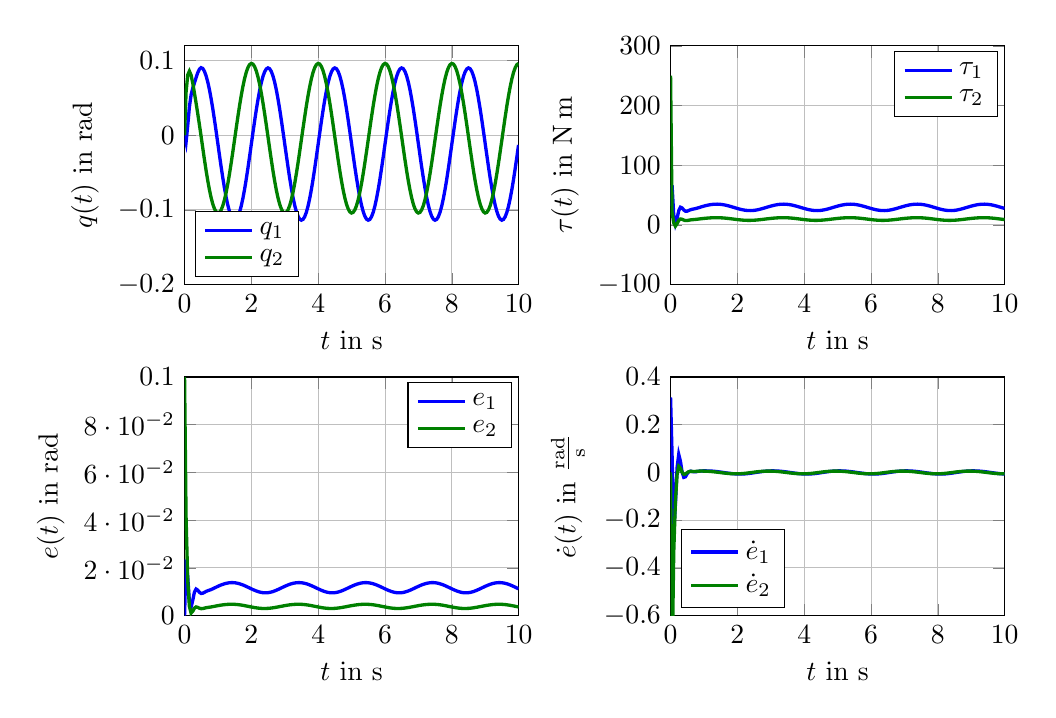
\begin{tikzpicture}

\begin{axis}[%
width=0.35\textwidth,
height=0.25\textwidth,
scale only axis,
xmin=0,
xmax=10,
xlabel={$t$ in $\mathrm{s}$},
xmajorgrids,
ymin=-0.2,
ymax=0.12,
ylabel={$q(t)$ in $\mathrm{rad}$},
ymajorgrids,
name=plot1,
legend style={at={(0.03,0.03)},anchor=south west,draw=black,fill=white,legend cell align=left}
]
\addplot [
color=blue,
solid,
line width=1.2pt
]
table[row sep=crcr]{
0 0\\
0.0446557465348323 -0.00953381112898908\\
0.0946557465348323 0.0129645884249693\\
0.144655746534832 0.0378850869707776\\
0.194655746534832 0.0539558594212379\\
0.244655746534832 0.0631140128130044\\
0.294655746534833 0.0700975490642797\\
0.344655746534833 0.0771851831161083\\
0.394655746534833 0.0838807449435335\\
0.444655746534833 0.088709124242084\\
0.494655746534833 0.0906767226600734\\
0.544655746534833 0.0896181911241804\\
0.594655746534833 0.0858406471215362\\
0.644655746534833 0.0797025136971008\\
0.694655746534833 0.0714396916222002\\
0.744655746534833 0.061208569238474\\
0.794655746534833 0.0491896107164486\\
0.844655746534833 0.0356444817788552\\
0.894655746534833 0.0209110764634811\\
0.944655746534833 0.00537012643436415\\
0.994655746534833 -0.0105839848251297\\
1.04465574653483 -0.0265574048888253\\
1.09465574653482 -0.0421614645071757\\
1.14465574653482 -0.0570164301292263\\
1.19465574653481 -0.0707584833269325\\
1.24465574653481 -0.0830492754828552\\
1.2946557465348 -0.0935856767871058\\
1.3446557465348 -0.102108050483801\\
1.39465574653479 -0.108406666027256\\
1.44465574653478 -0.112326553562168\\
1.49465574653478 -0.11377110167175\\
1.54465574653477 -0.112704429556196\\
1.59465574653477 -0.109152382271023\\
1.64465574653476 -0.103201999101029\\
1.69465574653476 -0.0949994110827336\\
1.74465574653475 -0.0847462314186947\\
1.79465574653475 -0.0726945655825271\\
1.84465574653474 -0.0591407930158804\\
1.89465574653473 -0.0444182836525333\\
1.94465574653473 -0.0288892255979424\\
1.99465574653472 -0.0129357570255309\\
2.04465574653472 0.00304938893107742\\
2.09465574653471 0.0186725066030543\\
2.14465574653471 0.0335485822223922\\
2.1946557465347 0.0473107732956305\\
2.2446557465347 0.0596194767592487\\
2.29465574653469 0.0701707635183995\\
2.34465574653469 0.0787039648471521\\
2.39465574653468 0.0850082097870495\\
2.44465574653467 0.0889277335129535\\
2.49465574653467 0.0903658053685954\\
2.54465574653466 0.0892871617661221\\
2.59465574653466 0.0857188722702532\\
2.64465574653465 0.0797496148438261\\
2.69465574653465 0.0715273855167407\\
2.74465574653464 0.0612557153615563\\
2.79465574653464 0.049188510492308\\
2.84465574653463 0.0356236664643062\\
2.89465574653462 0.0208956357022669\\
2.94465574653462 0.00536714544122325\\
2.99465574653461 -0.0105797247947834\\
3.04465574653461 -0.0265528912299075\\
3.0946557465346 -0.0421598223434229\\
3.1446557465346 -0.0570170870787937\\
3.19465574653459 -0.0707596798449352\\
3.24465574653459 -0.0830499107734423\\
3.29465574653458 -0.0935856551834358\\
3.34465574653458 -0.102107764873401\\
3.39465574653457 -0.108406456977161\\
3.44465574653456 -0.112326514865203\\
3.49465574653456 -0.113771160722779\\
3.54465574653455 -0.112704491110289\\
3.59465574653455 -0.109152404292153\\
3.64465574653454 -0.103201989834709\\
3.69465574653454 -0.0949993946596801\\
3.74465574653453 -0.0847462227911919\\
3.79465574653453 -0.0726945659484753\\
3.84465574653452 -0.0591407969517294\\
3.89465574653451 -0.0444182865058716\\
3.94465574653451 -0.0288892261118253\\
3.9946557465345 -0.012935756210094\\
4.04465574653452 0.00304938977193762\\
4.09465574653453 0.0186725069006652\\
4.14465574653455 0.0335485820939546\\
4.19465574653457 0.0473107730713384\\
4.24465574653458 0.0596194766419854\\
4.2946557465346 0.0701707635236293\\
4.34465574653462 0.078703964900834\\
4.39465574653463 0.0850082098259475\\
4.44465574653465 0.0889277335199953\\
4.49465574653467 0.0903658053574973\\
4.54465574653468 0.0892871617546322\\
4.5946557465347 0.0857188722661554\\
4.64465574653472 0.0797496148455556\\
4.69465574653473 0.071527385519794\\
4.74465574653475 0.0612557153631466\\
4.79465574653477 0.0491885104922117\\
4.84465574653478 0.0356236664635338\\
4.8946557465348 0.0208956357016864\\
4.94465574653482 0.0053671454410699\\
4.99465574653483 -0.0105797247946969\\
5.04465574653485 -0.0265528912298229\\
5.09465574653487 -0.0421598223434442\\
5.14465574653488 -0.0570170870788963\\
5.1946557465349 -0.0707596798450544\\
5.24465574653492 -0.0830499107735372\\
5.29465574653493 -0.0935856551835002\\
5.34465574653495 -0.102107764873446\\
5.39465574653497 -0.108406456977194\\
5.44465574653499 -0.112326514865224\\
5.494655746535 -0.113771160722784\\
5.54465574653502 -0.112704491110271\\
5.59465574653504 -0.10915240429211\\
5.64465574653505 -0.10320198983464\\
5.69465574653507 -0.094999394659585\\
5.74465574653509 -0.0847462227910719\\
5.7946557465351 -0.072694565948332\\
5.84465574653512 -0.0591407969515649\\
5.89465574653514 -0.0444182865056885\\
5.94465574653515 -0.0288892261116274\\
5.99465574653517 -0.012935756209886\\
6.04465574653519 0.00304938977214973\\
6.0946557465352 0.0186725069008722\\
6.14465574653522 0.0335485820941484\\
6.19465574653524 0.0473107730715136\\
6.24465574653525 0.0596194766421382\\
6.29465574653527 0.0701707635237567\\
6.34465574653529 0.0787039649009333\\
6.3946557465353 0.0850082098260161\\
6.44465574653532 0.0889277335200314\\
6.49465574653534 0.0903658053574998\\
6.54465574653535 0.089287161754601\\
6.59465574653537 0.0857188722660915\\
6.64465574653539 0.0797496148454604\\
6.6946557465354 0.07152738551967\\
6.74465574653542 0.0612557153629968\\
6.79465574653544 0.0491885104920398\\
6.84465574653545 0.0356236664633441\\
6.89465574653547 0.0208956357014835\\
6.94465574653549 0.00536714544085884\\
6.9946557465355 -0.0105797247949109\\
7.04465574653552 -0.0265528912300347\\
7.09465574653554 -0.0421598223436485\\
7.14465574653555 -0.057017087079088\\
7.19465574653557 -0.070759679845229\\
7.24465574653559 -0.0830499107736903\\
7.2946557465356 -0.0935856551836281\\
7.34465574653562 -0.102107764873545\\
7.39465574653564 -0.108406456977263\\
7.44465574653565 -0.11232651486526\\
7.49465574653567 -0.113771160722786\\
7.54465574653569 -0.11270449111024\\
7.5946557465357 -0.109152404292046\\
7.64465574653572 -0.103201989834545\\
7.69465574653574 -0.0949993946594613\\
7.74465574653575 -0.0847462227909224\\
7.79465574653577 -0.0726945659481603\\
7.84465574653579 -0.0591407969513752\\
7.8946557465358 -0.0444182865054857\\
7.94465574653582 -0.0288892261114163\\
7.99465574653584 -0.0129357562096718\\
8.04465574653581 0.00304938977235944\\
8.09465574653579 0.0186725069010652\\
8.14465574653576 0.0335485820943152\\
8.19465574653573 0.0473107730716507\\
8.2446557465357 0.0596194766422462\\
8.29465574653567 0.0701707635238377\\
8.34465574653565 0.0787039649009895\\
8.39465574653562 0.0850082098260499\\
8.44465574653559 0.0889277335200457\\
8.49465574653556 0.0903658053574984\\
8.54465574653554 0.0892871617545884\\
8.59465574653551 0.0857188722660727\\
8.64465574653548 0.0797496148454401\\
8.69465574653545 0.0715273855196526\\
8.74465574653543 0.0612557153629864\\
8.7946557465354 0.0491885104920399\\
8.84465574653537 0.0356236664633573\\
8.89465574653534 0.0208956357015115\\
8.94465574653531 0.00536714544090242\\
8.99465574653529 -0.0105797247948521\\
9.04465574653526 -0.0265528912299621\\
9.09465574653523 -0.0421598223435645\\
9.1446557465352 -0.057017087078996\\
9.19465574653518 -0.0707596798451332\\
9.24465574653515 -0.0830499107735957\\
9.29465574653512 -0.09358565518354\\
9.34465574653509 -0.102107764873469\\
9.39465574653507 -0.108406456977205\\
9.44465574653504 -0.112326514865226\\
9.49465574653501 -0.113771160722782\\
9.54465574653498 -0.112704491110269\\
9.59465574653495 -0.109152404292113\\
9.64465574653493 -0.103201989834651\\
9.6946557465349 -0.0949993946596085\\
9.74465574653487 -0.084746222791111\\
9.79465574653484 -0.0726945659483887\\
9.84465574653482 -0.0591407969516406\\
9.89465574653479 -0.0444182865057835\\
9.94465574653476 -0.0288892261117406\\
9.99465574653473 -0.0129357562100155\\
};
\addlegendentry{$q_1$};

\addplot [
color=green!50!black,
solid,
line width=1.2pt
]
table[row sep=crcr]{
0 0\\
0.0446557465348323 0.0574325651226278\\
0.0946557465348323 0.0809785654940199\\
0.144655746534832 0.0859725849186419\\
0.194655746534832 0.080807743781339\\
0.244655746534832 0.0700651136271607\\
0.294655746534833 0.0570106888148154\\
0.344655746534833 0.0432384576491328\\
0.394655746534833 0.0290240971336033\\
0.444655746534833 0.0141936811723833\\
0.494655746534833 -0.00124473855491904\\
0.544655746534833 -0.0169577123090355\\
0.594655746534833 -0.0324411674042166\\
0.644655746534833 -0.0472035820966997\\
0.694655746534833 -0.0608462300078268\\
0.744655746534833 -0.0730526785592832\\
0.794655746534833 -0.0835520647395752\\
0.844655746534833 -0.092100269454833\\
0.894655746534833 -0.0984852971774233\\
0.944655746534833 -0.102542830650572\\
0.994655746534833 -0.104168433905692\\
1.04465574653483 -0.103321943712817\\
1.09465574653482 -0.100026349815327\\
1.14465574653482 -0.0943648074991498\\
1.19465574653481 -0.0864776020166175\\
1.24465574653481 -0.0765589421445808\\
1.2946557465348 -0.0648527728245802\\
1.3446557465348 -0.051647115714025\\
1.39465574653479 -0.0372669987500232\\
1.44465574653478 -0.0220663380632326\\
1.49465574653478 -0.00641914656020144\\
1.54465574653477 0.00928966418089174\\
1.59465574653477 0.0246736999851924\\
1.64465574653476 0.0393545378122366\\
1.69465574653476 0.0529710083712482\\
1.74465574653475 0.0651880755309772\\
1.79465574653475 0.0757050806425439\\
1.84465574653474 0.0842631398167411\\
1.89465574653473 0.090651510808684\\
1.94465574653473 0.0947127761376326\\
1.99465574653472 0.0963467188721231\\
2.04465574653472 0.0955127984286191\\
2.09465574653471 0.0922311667730572\\
2.14465574653471 0.0865822002249452\\
2.1946557465347 0.078704557444608\\
2.2446557465347 0.0687918089532509\\
2.29465574653469 0.0570877169531669\\
2.34465574653469 0.0438802759207504\\
2.39465574653468 0.0294946541894958\\
2.44465574653467 0.0142852041694563\\
2.49465574653467 -0.00137326659077613\\
2.54465574653466 -0.0170947503623563\\
2.59465574653466 -0.0324915906952818\\
2.64465574653465 -0.0471840900279074\\
2.69465574653465 -0.0608099287747004\\
2.74465574653464 -0.0730331541521556\\
2.79465574653464 -0.0835525075437112\\
2.84465574653463 -0.0921088771879743\\
2.89465574653462 -0.098491687674879\\
2.94465574653462 -0.102544067942123\\
2.99465574653461 -0.104166673658122\\
3.04465574653461 -0.103320076445383\\
3.0946557465346 -0.10002566984574\\
3.1446557465346 -0.0943650790308306\\
3.19465574653459 -0.0864780971257621\\
3.24465574653459 -0.0765592050675596\\
3.29465574653458 -0.0648527638315915\\
3.34465574653458 -0.0516469974345943\\
3.39465574653457 -0.0372669121943522\\
3.44465574653456 -0.0220663220573588\\
3.49465574653456 -0.0064191710277276\\
3.54465574653455 0.00928963868193905\\
3.59465574653455 0.0246736908593863\\
3.64465574653454 0.0393545416456822\\
3.69465574653454 0.0529710151731808\\
3.74465574653453 0.0651880791083202\\
3.79465574653453 0.0757050804953777\\
3.84465574653452 0.0842631381883377\\
3.89465574653451 0.0906515096260371\\
3.94465574653451 0.0947127759232375\\
3.9946557465345 0.096346719209038\\
4.04465574653452 0.0955127987769308\\
4.09465574653453 0.0922311668966819\\
4.14465574653455 0.0865822001719971\\
4.19465574653457 0.0787045573517811\\
4.24465574653458 0.0687918089046831\\
4.2946557465346 0.0570877169553427\\
4.34465574653462 0.0438802759430111\\
4.39465574653463 0.029494654205632\\
4.44465574653465 0.0142852041723879\\
4.49465574653467 -0.00137326659536685\\
4.54465574653468 -0.0170947503671159\\
4.5946557465347 -0.0324915906969856\\
4.64465574653472 -0.0471840900272021\\
4.69465574653473 -0.0608099287734488\\
4.74465574653475 -0.0730331541515089\\
4.79465574653477 -0.0835525075437597\\
4.84465574653478 -0.0921088771882975\\
4.8946557465348 -0.0984916876751153\\
4.94465574653482 -0.102544067942173\\
4.99465574653483 -0.10416667365806\\
5.04465574653485 -0.103320076445308\\
5.09465574653487 -0.100025669845694\\
5.14465574653488 -0.0943650790308037\\
5.1946557465349 -0.0864780971257271\\
5.24465574653492 -0.0765592050675004\\
5.29465574653493 -0.0648527638315071\\
5.34465574653495 -0.0516469974344911\\
5.39465574653497 -0.0372669121942366\\
5.44465574653499 -0.022066322057234\\
5.494655746535 -0.00641917102759523\\
5.54465574653502 0.00928963868207716\\
5.59465574653504 0.024673690859527\\
5.64465574653505 0.0393545416458213\\
5.69465574653507 0.0529710151733136\\
5.74465574653509 0.065188079108442\\
5.7946557465351 0.0757050804954839\\
5.84465574653512 0.084263138188424\\
5.89465574653514 0.0906515096260996\\
5.94465574653515 0.0947127759232727\\
5.99465574653517 0.0963467192090427\\
6.04465574653519 0.0955127987769039\\
6.0946557465352 0.0922311668966231\\
6.14465574653522 0.0865822001719072\\
6.19465574653524 0.0787045573516619\\
6.24465574653525 0.0687918089045379\\
6.29465574653527 0.0570877169551754\\
6.34465574653529 0.043880275942826\\
6.3946557465353 0.0294946542054336\\
6.44465574653532 0.0142852041721809\\
6.49465574653534 -0.00137326659557726\\
6.54465574653535 -0.0170947503673246\\
6.59465574653537 -0.0324915906971874\\
6.64465574653539 -0.047184090027392\\
6.6946557465354 -0.0608099287736221\\
6.74465574653542 -0.0730331541516614\\
6.79465574653544 -0.0835525075438877\\
6.84465574653545 -0.0921088771883977\\
6.89465574653547 -0.0984916876751853\\
6.94465574653549 -0.102544067942211\\
6.9946557465355 -0.104166673658066\\
7.04465574653552 -0.10332007644528\\
7.09465574653554 -0.100025669845634\\
7.14465574653555 -0.0943650790307129\\
7.19465574653557 -0.0864780971256078\\
7.24465574653559 -0.0765592050673554\\
7.2946557465356 -0.06485276383134\\
7.34465574653562 -0.0516469974343061\\
7.39465574653564 -0.0372669121940382\\
7.44465574653565 -0.0220663220570272\\
7.49465574653567 -0.00641917102738495\\
7.54465574653569 0.00928963868228566\\
7.5946557465357 0.0246736908597286\\
7.64465574653572 0.039354541646011\\
7.69465574653574 0.0529710151734869\\
7.74465574653575 0.0651880791085944\\
7.79465574653577 0.0757050804956118\\
7.84465574653579 0.0842631381885243\\
7.8946557465358 0.0906515096261697\\
7.94465574653582 0.0947127759233108\\
7.99465574653584 0.0963467192090481\\
8.04465574653581 0.0955127987768784\\
8.09465574653579 0.0922311668965706\\
8.14465574653576 0.086582200171831\\
8.19465574653573 0.0787045573515675\\
8.2446557465357 0.0687918089044319\\
8.29465574653567 0.0570877169550641\\
8.34465574653565 0.0438802759427152\\
8.39465574653562 0.029494654205328\\
8.44465574653559 0.0142852041720845\\
8.49465574653556 -0.00137326659566155\\
8.54465574653554 -0.0170947503673946\\
8.59465574653551 -0.0324915906972417\\
8.64465574653548 -0.0471840900274307\\
8.69465574653545 -0.0608099287736461\\
8.74465574653543 -0.0730331541516725\\
8.7946557465354 -0.0835525075438887\\
8.84465574653537 -0.092108877188392\\
8.89465574653534 -0.098491687675177\\
8.94465574653531 -0.102544067942204\\
8.99465574653529 -0.104166673658065\\
9.04465574653526 -0.10332007644529\\
9.09465574653523 -0.100025669845659\\
9.1446557465352 -0.0943650790307558\\
9.19465574653518 -0.0864780971256718\\
9.24465574653515 -0.0765592050674426\\
9.29465574653512 -0.0648527638314514\\
9.34465574653509 -0.0516469974344416\\
9.39465574653507 -0.0372669121941964\\
9.44465574653504 -0.0220663220572058\\
9.49465574653501 -0.00641917102758031\\
9.54465574653498 0.00928963868207821\\
9.59465574653495 0.0246736908595147\\
9.64465574653493 0.0393545416457973\\
9.6946557465349 0.0529710151732804\\
9.74465574653487 0.0651880791084028\\
9.79465574653484 0.0757050804954426\\
9.84465574653482 0.0842631381883853\\
9.89465574653479 0.0906515096260682\\
9.94465574653476 0.0947127759232534\\
9.99465574653473 0.0963467192090404\\
};
\addlegendentry{$q_2$};

\end{axis}

\begin{axis}[%
width=0.35\textwidth,
height=0.25\textwidth,
scale only axis,
xmin=0,
xmax=10,
xlabel={$t$ in $\mathrm{s}$},
xmajorgrids,
ymin=0,
ymax=0.1,
ylabel={$e(t)$ in $\mathrm{rad}$},
ymajorgrids,
name=plot3,
at=(plot1.below south west),
anchor=above north west,
legend style={draw=black,fill=white,legend cell align=left}
]
\addplot [
color=blue,
solid,
line width=1.2pt
]
table[row sep=crcr]{
0 0\\
0.0446557465348323 0.0235168546332067\\
0.0946557465348323 0.0163360575102949\\
0.144655746534832 0.00601168224933834\\
0.194655746534832 0.00345614894050583\\
0.244655746534832 0.00639956050496945\\
0.294655746534833 0.00980593433251263\\
0.344655746534833 0.0111407214138157\\
0.394655746534833 0.0106927038131246\\
0.444655746534833 0.00978315656163782\\
0.494655746534833 0.00930918336018523\\
0.544655746534833 0.00939935527219903\\
0.594655746534833 0.00977039903828929\\
0.644655746534833 0.010147770954846\\
0.694655746534833 0.0104374193177386\\
0.744655746534833 0.0106792817835635\\
0.794655746534833 0.010938862913426\\
0.844655746534833 0.0112440518831259\\
0.894655746534833 0.0115829659177271\\
0.944655746534833 0.0119293135011019\\
0.994655746534833 0.0122628526900929\\
1.04465574653483 0.012574361384609\\
1.09465574653482 0.0128608185719144\\
1.14465574653482 0.0131196609091147\\
1.19465574653481 0.013346474965194\\
1.24465574653481 0.0135357021648872\\
1.2946557465348 0.0136821933903195\\
1.3446557465348 0.0137821459538828\\
1.39465574653479 0.0138332172706018\\
1.44465574653478 0.013834272758449\\
1.49465574653478 0.0137851956514917\\
1.54465574653477 0.0136868831598138\\
1.59465574653477 0.0135413361111912\\
1.64465574653476 0.0133517144490727\\
1.69465574653476 0.013122300142781\\
1.74465574653475 0.0128583803966393\\
1.79465574653475 0.0125660919526306\\
1.84465574653474 0.0122522593538736\\
1.89465574653473 0.0119242412712959\\
1.94465574653473 0.0115897856624442\\
1.99465574653472 0.0112568891605332\\
2.04465574653472 0.0109336545731047\\
2.09465574653471 0.0106281393321739\\
2.14465574653471 0.0103481869976884\\
2.1946557465347 0.0101012350660796\\
2.2446557465347 0.0098940965586943\\
2.29465574653469 0.00973271987836605\\
2.34465574653469 0.00962193968275019\\
2.39465574653468 0.00956523896959297\\
2.44465574653467 0.00956454729075978\\
2.49465574653467 0.00962010065166242\\
2.54465574653466 0.00973038463026481\\
2.59465574653466 0.00989217388958843\\
2.64465574653465 0.0101006698081457\\
2.69465574653465 0.0103497254232317\\
2.74465574653464 0.0106321356605231\\
2.79465574653464 0.010939963137616\\
2.84465574653463 0.0112648671977313\\
2.89465574653462 0.0115984066790032\\
2.94465574653462 0.011932294494309\\
2.99465574653461 0.0122585926598156\\
3.04465574653461 0.0125698477257597\\
3.0946557465346 0.0128591764082277\\
3.1446557465346 0.0131203178587442\\
3.19465574653459 0.0133476714832534\\
3.24465574653459 0.0135363374555242\\
3.29465574653458 0.0136821717866911\\
3.34465574653458 0.0137818603435149\\
3.39465574653457 0.0138330082205299\\
3.44465574653456 0.0138342340614953\\
3.49465574653456 0.0137852547025218\\
3.54465574653455 0.0136869447138968\\
3.59465574653455 0.0135413581323015\\
3.64465574653454 0.0133517051827224\\
3.69465574653454 0.0131222837196878\\
3.74465574653453 0.0128583717690884\\
3.79465574653453 0.0125660923185235\\
3.84465574653452 0.0122522632896614\\
3.89465574653451 0.0119242441245687\\
3.94465574653451 0.0115897861762589\\
3.9946557465345 0.0112568883450272\\
4.04465574653452 0.010933653732182\\
4.09465574653453 0.0106281390345094\\
4.14465574653455 0.0103481871260818\\
4.19465574653457 0.0101012352903371\\
4.24465574653458 0.00989409667593235\\
4.2946557465346 0.00973271987311926\\
4.34465574653462 0.00962193962905838\\
4.39465574653463 0.00956523893069033\\
4.44465574653465 0.00956454728371665\\
4.49465574653467 0.00962010066276042\\
4.54465574653468 0.00973038464175381\\
4.5946557465347 0.0098921738936822\\
4.64465574653472 0.0101006698064072\\
4.69465574653473 0.0103497254201626\\
4.74465574653475 0.0106321356589087\\
4.79465574653477 0.0109399631376792\\
4.84465574653478 0.0112648671984607\\
4.8946557465348 0.0115984066795312\\
4.94465574653482 0.0119322944944008\\
4.99465574653483 0.0122585926596597\\
5.04465574653485 0.0125698477255994\\
5.09465574653487 0.0128591764081693\\
5.14465574653488 0.0131203178587658\\
5.1946557465349 0.0133476714832929\\
5.24465574653492 0.0135363374555441\\
5.29465574653493 0.0136821717866886\\
5.34465574653495 0.0137818603435041\\
5.39465574653497 0.0138330082205224\\
5.44465574653499 0.0138342340614943\\
5.494655746535 0.0137852547025244\\
5.54465574653502 0.0136869447138997\\
5.59465574653504 0.0135413581323033\\
5.64465574653505 0.0133517051827234\\
5.69465574653507 0.0131222837196886\\
5.74465574653509 0.0128583717690896\\
5.7946557465351 0.0125660923185249\\
5.84465574653512 0.0122522632896631\\
5.89465574653514 0.0119242441245701\\
5.94465574653515 0.0115897861762601\\
5.99465574653517 0.011256888345028\\
6.04465574653519 0.0109336537321778\\
6.0946557465352 0.0106281390345029\\
6.14465574653522 0.0103481871260766\\
6.19465574653524 0.0101012352903338\\
6.24465574653525 0.0098940966759305\\
6.29465574653527 0.00973271987311795\\
6.34465574653529 0.00962193962905748\\
6.3946557465353 0.00956523893068986\\
6.44465574653532 0.00956454728371688\\
6.49465574653534 0.00962010066276148\\
6.54465574653535 0.00973038464175564\\
6.59465574653537 0.00989217389368469\\
6.64465574653539 0.0101006698064102\\
6.6946557465354 0.0103497254201662\\
6.74465574653542 0.0106321356589127\\
6.79465574653544 0.0109399631376836\\
6.84465574653545 0.0112648671984652\\
6.89465574653547 0.0115984066795359\\
6.94465574653549 0.0119322944944053\\
6.9946557465355 0.0122585926596641\\
7.04465574653552 0.0125698477256034\\
7.09465574653554 0.0128591764081732\\
7.14465574653555 0.0131203178587689\\
7.19465574653557 0.0133476714832956\\
7.24465574653559 0.0135363374555463\\
7.2946557465356 0.0136821717866902\\
7.34465574653562 0.0137818603435051\\
7.39465574653564 0.0138330082205227\\
7.44465574653565 0.0138342340614939\\
7.49465574653567 0.0137852547025234\\
7.54465574653569 0.013686944713898\\
7.5946557465357 0.0135413581323011\\
7.64465574653572 0.0133517051827205\\
7.69465574653574 0.0131222837196854\\
7.74465574653575 0.0128583717690858\\
7.79465574653577 0.0125660923185209\\
7.84465574653579 0.0122522632896586\\
7.8946557465358 0.0119242441245657\\
7.94465574653582 0.0115897861762554\\
7.99465574653584 0.0112568883450237\\
8.04465574653581 0.0109336537321633\\
8.09465574653579 0.0106281390344852\\
8.14465574653576 0.0103481871260617\\
8.19465574653573 0.010101235290324\\
8.2446557465357 0.00989409667592411\\
8.29465574653567 0.00973271987311361\\
8.34465574653565 0.0096219396290544\\
8.39465574653562 0.00956523893068853\\
8.44465574653559 0.00956454728371743\\
8.49465574653556 0.0096201006627641\\
8.54465574653554 0.00973038464176013\\
8.59465574653551 0.00989217389369061\\
8.64465574653548 0.0101006698064174\\
8.69465574653545 0.0103497254201744\\
8.74465574653543 0.0106321356589219\\
8.7946557465354 0.0109399631376929\\
8.84465574653537 0.0112648671984749\\
8.89465574653534 0.0115984066795455\\
8.94465574653531 0.0119322944944149\\
8.99465574653529 0.0122585926596729\\
9.04465574653526 0.0125698477256118\\
9.09465574653523 0.0128591764081806\\
9.1446557465352 0.0131203178587755\\
9.19465574653518 0.013347671483301\\
9.24465574653515 0.0135363374555505\\
9.29465574653512 0.0136821717866934\\
9.34465574653509 0.013781860343507\\
9.39465574653507 0.0138330082205234\\
9.44465574653504 0.0138342340614935\\
9.49465574653501 0.0137852547025221\\
9.54465574653498 0.0136869447138959\\
9.59465574653495 0.0135413581322983\\
9.64465574653493 0.0133517051827171\\
9.6946557465349 0.0131222837196815\\
9.74465574653487 0.0128583717690817\\
9.79465574653484 0.0125660923185168\\
9.84465574653482 0.0122522632896546\\
9.89465574653479 0.0119242441245618\\
9.94465574653476 0.0115897861762518\\
9.99465574653473 0.0112568883450207\\
};
\addlegendentry{$e_1$};

\addplot [
color=green!50!black,
solid,
line width=1.2pt
]
table[row sep=crcr]{
0 0.1\\
0.0446557465348323 0.0415849812737517\\
0.0946557465348323 0.0146324806658056\\
0.144655746534832 0.00387769973330504\\
0.194655746534832 0.0010693671585999\\
0.244655746534832 0.00182273739487693\\
0.294655746534833 0.00311778481505923\\
0.344655746534833 0.00365007601284845\\
0.394655746534833 0.00346994524760496\\
0.444655746534833 0.00310575876308293\\
0.494655746534833 0.00292360641988246\\
0.544655746534833 0.00297466880481779\\
0.594655746534833 0.00314052146895225\\
0.644655746534833 0.00330681287658364\\
0.694655746534833 0.0034342216460829\\
0.744655746534833 0.0035391052413092\\
0.794655746534833 0.00364858134278279\\
0.844655746534833 0.0037743649249089\\
0.894655746534833 0.00391184842076518\\
0.944655746534833 0.00405054984685002\\
0.994655746534833 0.0041825278854334\\
1.04465574653483 0.00430439731643752\\
1.09465574653482 0.00441530365550045\\
1.14465574653482 0.00451452284720086\\
1.19465574653481 0.00460049107667485\\
1.24465574653481 0.00467109112253751\\
1.2946557465348 0.0047242991946975\\
1.3446557465348 0.00475858205203344\\
1.39465574653479 0.00477295636880214\\
1.44465574653478 0.0047668981277514\\
1.49465574653478 0.00474027869522103\\
1.54465574653477 0.0046933793233075\\
1.59465574653477 0.00462694595005229\\
1.64465574653476 0.00454223140785948\\
1.69465574653476 0.0044409999904761\\
1.74465574653475 0.00432549778697833\\
1.79465574653475 0.00419840275423201\\
1.84465574653474 0.0040627647131693\\
1.89465574653473 0.00392193794796415\\
1.94465574653473 0.00377950466608361\\
1.99465574653472 0.00363918714813495\\
2.04465574653472 0.0035047479677654\\
2.09465574653471 0.00337987938677937\\
2.14465574653471 0.00326808442701902\\
2.1946557465347 0.00317255349535447\\
2.2446557465347 0.00309604206881646\\
2.29465574653469 0.0030407566767434\\
2.34465574653469 0.00300825774127181\\
2.39465574653468 0.00299938819175797\\
2.44465574653467 0.00301423576605904\\
2.49465574653467 0.0030521344557911\\
2.54465574653466 0.00311170685819133\\
2.59465574653466 0.00319094476007023\\
2.64465574653465 0.00328732080784244\\
2.69465574653465 0.00339792041300449\\
2.74465574653464 0.00351958083422496\\
2.79465574653464 0.00364902414695605\\
2.84465574653463 0.0037829726580801\\
2.89465574653462 0.00391823891824215\\
2.94465574653462 0.00405178713841288\\
2.99465574653461 0.00418076763786478\\
3.04465574653461 0.0043025300489932\\
3.0946557465346 0.00441462368589307\\
3.1446557465346 0.00451479437885126\\
3.19465574653459 0.0046009861857798\\
3.24465574653459 0.00467135404546809\\
3.29465574653458 0.00472429020165354\\
3.34465574653458 0.00475846377254158\\
3.39465574653457 0.00477286981306577\\
3.44465574653456 0.0047668821218094\\
3.49465574653456 0.00474030316267799\\
3.54465574653455 0.00469340482219165\\
3.59465574653455 0.00462695507579238\\
3.64465574653454 0.00454222757435163\\
3.69465574653454 0.00444099318848673\\
3.74465574653453 0.00432549420958553\\
3.79465574653453 0.00419840290135665\\
3.84465574653452 0.00406276634154026\\
3.89465574653451 0.0039219391305885\\
3.94465574653451 0.00377950488046677\\
3.9946557465345 0.00363918681121891\\
4.04465574653452 0.00350474761946244\\
4.09465574653453 0.00337987926317113\\
4.14465574653455 0.00326808447998865\\
4.19465574653457 0.00317255358820566\\
4.24465574653458 0.00309604211740873\\
4.2946557465346 0.00304075667459017\\
4.34465574653462 0.00300825771902986\\
4.39465574653463 0.0029993881756353\\
4.44465574653465 0.00301423576313462\\
4.49465574653467 0.0030521344603822\\
4.54465574653468 0.00311170686294444\\
4.5946557465347 0.00319094476176091\\
4.64465574653472 0.00328732080711869\\
4.69465574653473 0.00339792041173029\\
4.74465574653475 0.00351958083355336\\
4.79465574653477 0.0036490241469796\\
4.84465574653478 0.00378297265838048\\
4.8946557465348 0.00391823891846038\\
4.94465574653482 0.0040517871384516\\
4.99465574653483 0.00418076763780183\\
5.04465574653485 0.0043025300489293\\
5.09465574653487 0.00441462368587216\\
5.14465574653488 0.00451479437886397\\
5.1946557465349 0.00460098618580068\\
5.24465574653492 0.0046713540454814\\
5.29465574653493 0.00472429020165811\\
5.34465574653495 0.00475846377254276\\
5.39465574653497 0.00477286981306855\\
5.44465574653499 0.00476688212181475\\
5.494655746535 0.00474030316268483\\
5.54465574653502 0.00469340482219846\\
5.59465574653504 0.00462695507579804\\
5.64465574653505 0.00454222757435663\\
5.69465574653507 0.00444099318849079\\
5.74465574653509 0.00432549420958903\\
5.7946557465351 0.00419840290135928\\
5.84465574653512 0.00406276634154219\\
5.89465574653514 0.00392193913058934\\
5.94465574653515 0.00377950488046656\\
5.99465574653517 0.00363918681121768\\
6.04465574653519 0.00350474761946006\\
6.0946557465352 0.00337987926316838\\
6.14465574653522 0.00326808447998639\\
6.19465574653524 0.0031725535882044\\
6.24465574653525 0.00309604211740799\\
6.29465574653527 0.00304075667458987\\
6.34465574653529 0.00300825771902952\\
6.3946557465353 0.0029993881756353\\
6.44465574653532 0.00301423576313477\\
6.49465574653534 0.00305213446038287\\
6.54465574653535 0.00311170686294525\\
6.59465574653537 0.00319094476176214\\
6.64465574653539 0.00328732080711995\\
6.6946557465354 0.00339792041173191\\
6.74465574653542 0.00351958083355507\\
6.79465574653544 0.00364902414698152\\
6.84465574653545 0.00378297265838232\\
6.89465574653547 0.00391823891846226\\
6.94465574653549 0.00405178713845337\\
6.9946557465355 0.00418076763780356\\
7.04465574653552 0.00430253004893087\\
7.09465574653554 0.0044146236858735\\
7.14465574653555 0.00451479437886526\\
7.19465574653557 0.00460098618580185\\
7.24465574653559 0.00467135404548234\\
7.2946557465356 0.0047242902016588\\
7.34465574653562 0.0047584637725432\\
7.39465574653564 0.00477286981306874\\
7.44465574653565 0.00476688212181466\\
7.49465574653567 0.00474030316268447\\
7.54465574653569 0.00469340482219748\\
7.5946557465357 0.00462695507579716\\
7.64465574653572 0.00454222757435518\\
7.69465574653574 0.00444099318848946\\
7.74465574653575 0.00432549420958726\\
7.79465574653577 0.00419840290135762\\
7.84465574653579 0.00406276634154022\\
7.8946557465358 0.00392193913058746\\
7.94465574653582 0.00377950488046465\\
7.99465574653584 0.00363918681121587\\
8.04465574653581 0.00350474761945793\\
8.09465574653579 0.00337987926316727\\
8.14465574653576 0.00326808447998836\\
8.19465574653573 0.00317255358820946\\
8.2446557465357 0.00309604211741575\\
8.29465574653567 0.00304075667459922\\
8.34465574653565 0.00300825771904024\\
8.39465574653562 0.00299938817564651\\
8.44465574653559 0.00301423576314695\\
8.49465574653556 0.00305213446039544\\
8.54465574653554 0.00311170686295821\\
8.59465574653551 0.00319094476177441\\
8.64465574653548 0.00328732080713184\\
8.69465574653545 0.00339792041174276\\
8.74465574653543 0.00351958083356493\\
8.7946557465354 0.00364902414698956\\
8.84465574653537 0.00378297265838885\\
8.89465574653534 0.0039182389184669\\
8.94465574653531 0.00405178713845608\\
8.99465574653529 0.00418076763780421\\
9.04465574653526 0.00430253004892955\\
9.09465574653523 0.00441462368587024\\
9.1446557465352 0.00451479437886004\\
9.19465574653518 0.00460098618579491\\
9.24465574653515 0.00467135404547395\\
9.29465574653512 0.00472429020164896\\
9.34465574653509 0.00475846377253236\\
9.39465574653507 0.00477286981305725\\
9.44465574653504 0.00476688212180287\\
9.49465574653501 0.00474030316267236\\
9.54465574653498 0.00469340482218575\\
9.59465574653495 0.00462695507578612\\
9.64465574653493 0.00454222757434514\\
9.6946557465349 0.00444099318848036\\
9.74465574653487 0.00432549420957969\\
9.79465574653484 0.00419840290135179\\
9.84465574653482 0.00406276634153624\\
9.89465574653479 0.00392193913058528\\
9.94465574653476 0.00377950488046444\\
9.99465574653473 0.00363918681121767\\
};
\addlegendentry{$e_2$};

\end{axis}

\begin{axis}[%
width=0.35\textwidth,
height=0.25\textwidth,
scale only axis,
xmin=0,
xmax=10,
xlabel={$t$ in $\mathrm{s}$},
xmajorgrids,
ymin=-0.6,
ymax=0.4,
ylabel={$\dot{e}(t)$ in $\mathrm{\frac{rad}{s}}$},
ymajorgrids,
name=plot2,
at=(plot3.right of south east),
anchor=left of south west,
legend style={at={(0.03,0.03)},anchor=south west,draw=black,fill=white,legend cell align=left}
]
\addplot [
color=blue,
solid,
line width=1.2pt
]
table[row sep=crcr]{
0 0.314159265358979\\
0.0446557465348323 0.0750359554030567\\
0.0946557465348323 -0.246613707836071\\
0.144655746534832 -0.136379149343452\\
0.194655746534832 0.0198396787332904\\
0.244655746534832 0.0755603666084879\\
0.294655746534833 0.0478075328847762\\
0.344655746534833 0.00221435094663827\\
0.394655746534833 -0.0207049539895125\\
0.444655746534833 -0.0183913541295104\\
0.494655746534833 -0.00624133398557152\\
0.544655746534833 0.00278932999009926\\
0.594655746534833 0.0052591644133175\\
0.644655746534833 0.00400107107343953\\
0.694655746534833 0.00262933989590947\\
0.744655746534833 0.0026965133932188\\
0.794655746534833 0.00384477834097086\\
0.844655746534833 0.00513104841889589\\
0.894655746534833 0.00597862035013558\\
0.944655746534833 0.00634241923613194\\
0.994655746534833 0.00643030002210737\\
1.04465574653483 0.00641912877248924\\
1.09465574653482 0.00635582371319743\\
1.14465574653482 0.00620213326078423\\
1.19465574653481 0.00591083862561104\\
1.24465574653481 0.00546515906405526\\
1.2946557465348 0.00487688404262718\\
1.3446557465348 0.00416860267168453\\
1.39465574653479 0.00336115649011383\\
1.44465574653478 0.00247162573552193\\
1.49465574653478 0.00151694463307763\\
1.54465574653477 0.000517171862953934\\
1.59465574653477 -0.000504026320729586\\
1.64465574653476 -0.00152094986075421\\
1.69465574653476 -0.00250782447274214\\
1.74465574653475 -0.00344011078369189\\
1.79465574653475 -0.00429503941548648\\
1.84465574653474 -0.0050517140610663\\
1.89465574653473 -0.00569112770730479\\
1.94465574653473 -0.00619626497819564\\
1.99465574653472 -0.00655233763470908\\
2.04465574653472 -0.0067471665121876\\
2.09465574653471 -0.00677172482742555\\
2.14465574653471 -0.00662083760137822\\
2.1946557465347 -0.0062939781690895\\
2.2446557465347 -0.0057960390916936\\
2.29465574653469 -0.00513791168201294\\
2.34465574653469 -0.00433670407211903\\
2.39465574653468 -0.00341546511264035\\
2.44465574653467 -0.00240235252703937\\
2.49465574653467 -0.0013292749234317\\
2.54465574653466 -0.000230131386760091\\
2.59465574653466 0.000861149358972857\\
2.64465574653465 0.00191252341110879\\
2.69465574653465 0.00289545371421698\\
2.74465574653464 0.00378604244387257\\
2.79465574653464 0.00456556455613977\\
2.84465574653463 0.00522040168946797\\
2.89465574653462 0.0057414804998277\\
2.94465574653462 0.00612339844109244\\
2.99465574653461 0.0063634576289906\\
3.04465574653461 0.00646081880536348\\
3.0946557465346 0.00641593805040108\\
3.1446557465346 0.0062303721055561\\
3.19465574653459 0.00590695121088192\\
3.24465574653459 0.00545023852740953\\
3.29465574653458 0.00486713690987092\\
3.34465574653458 0.00416747661813849\\
3.39465574653457 0.00336442522369902\\
3.44465574653456 0.00247460084511775\\
3.49465574653456 0.00151783316607073\\
3.54465574653455 0.000516589756247215\\
3.59465574653455 -0.000504848161543642\\
3.64465574653454 -0.00152133137019767\\
3.69465574653454 -0.00250776764522376\\
3.74465574653453 -0.00343990557849136\\
3.79465574653453 -0.00429490665035864\\
3.84465574653452 -0.00505169955567814\\
3.89465574653451 -0.00569117286946536\\
3.94465574653451 -0.00619630563230089\\
3.9946557465345 -0.0065523495790199\\
4.04465574653452 -0.00674715843120888\\
4.09465574653453 -0.00677171359532519\\
4.14465574653455 -0.00662083243394462\\
4.19465574653457 -0.00629397897110856\\
4.24465574653458 -0.00579604189291794\\
4.2946557465346 -0.00513791348656745\\
4.34465574653462 -0.00433670426742308\\
4.39465574653463 -0.00341546449765695\\
4.44465574653465 -0.00240235197310447\\
4.49465574653467 -0.00132927475972542\\
4.54465574653468 -0.000230131496239315\\
4.5946557465347 0.000861149205655637\\
4.64465574653472 0.00191252334012787\\
4.69465574653473 0.00289545372493943\\
4.74465574653475 0.00378604248224335\\
4.79465574653477 0.00456556458102092\\
4.84465574653478 0.00522040169230853\\
4.8946557465348 0.00574148049154138\\
4.94465574653482 0.00612339843365017\\
4.99465574653483 0.00636345762691121\\
5.04465574653485 0.00646081880702293\\
5.09465574653487 0.00641593805264107\\
5.14465574653488 0.00623037210665339\\
5.1946557465349 0.00590695121085499\\
5.24465574653492 0.00545023852700022\\
5.29465574653493 0.00486713690963325\\
5.34465574653495 0.00416747661818317\\
5.39465574653497 0.00336442522387223\\
5.44465574653499 0.00247460084525557\\
5.494655746535 0.00151783316611141\\
5.54465574653502 0.000516589756213687\\
5.59465574653504 -0.000504848161606716\\
5.64465574653505 -0.00152133137026825\\
5.69465574653507 -0.00250776764530036\\
5.74465574653509 -0.00343990557858251\\
5.7946557465351 -0.00429490665046856\\
5.84465574653512 -0.00505169955580698\\
5.89465574653514 -0.00569117286960635\\
5.94465574653515 -0.00619630563244927\\
5.99465574653517 -0.00655234957917028\\
6.04465574653519 -0.00674715843129942\\
6.0946557465352 -0.00677171359533396\\
6.14465574653522 -0.0066208324339127\\
6.19465574653524 -0.00629397897107736\\
6.24465574653525 -0.00579604189290261\\
6.29465574653527 -0.00513791348656334\\
6.34465574653529 -0.00433670426741883\\
6.3946557465353 -0.00341546449764768\\
6.44465574653532 -0.00240235197308876\\
6.49465574653534 -0.0013292747597089\\
6.54465574653535 -0.000230131496223453\\
6.59465574653537 0.000861149205669959\\
6.64465574653539 0.0019125233401418\\
6.6946557465354 0.00289545372495184\\
6.74465574653542 0.00378604248225525\\
6.79465574653544 0.00456556458103113\\
6.84465574653545 0.00522040169231597\\
6.89465574653547 0.00574148049154705\\
6.94465574653549 0.00612339843365423\\
6.9946557465355 0.00636345762691387\\
7.04465574653552 0.00646081880702259\\
7.09465574653554 0.00641593805263979\\
7.14465574653555 0.00623037210665056\\
7.19465574653557 0.00590695121085072\\
7.24465574653559 0.00545023852699336\\
7.2946557465356 0.00486713690962395\\
7.34465574653562 0.00416747661817216\\
7.39465574653564 0.00336442522386045\\
7.44465574653565 0.00247460084524317\\
7.49465574653567 0.00151783316609884\\
7.54465574653569 0.00051658975620044\\
7.5946557465357 -0.000504848161620899\\
7.64465574653572 -0.0015213313702814\\
7.69465574653574 -0.00250776764531396\\
7.74465574653575 -0.00343990557859494\\
7.79465574653577 -0.00429490665048082\\
7.84465574653579 -0.00505169955581636\\
7.8946557465358 -0.00569117286961424\\
7.94465574653582 -0.00619630563245416\\
7.99465574653584 -0.00655234957917367\\
8.04465574653581 -0.00674715843118129\\
8.09465574653579 -0.00677171359505924\\
8.14465574653576 -0.00662083243357275\\
8.19465574653573 -0.00629397897076328\\
8.2446557465357 -0.00579604189265079\\
8.29465574653567 -0.00513791348636525\\
8.34465574653565 -0.00433670426725907\\
8.39465574653562 -0.00341546449752056\\
8.44465574653559 -0.00240235197299991\\
8.49465574653556 -0.00132927475966301\\
8.54465574653554 -0.000230131496225874\\
8.59465574653551 0.000861149205618653\\
8.64465574653548 0.00191252334004344\\
8.69465574653545 0.00289545372481131\\
8.74465574653543 0.00378604248207504\\
8.7946557465354 0.00456556458081525\\
8.84465574653537 0.005220401692072\\
8.89465574653534 0.00574148049128004\\
8.94465574653531 0.00612339843337106\\
8.99465574653529 0.00636345762662066\\
9.04465574653526 0.00646081880672844\\
9.09465574653523 0.00641593805235097\\
9.1446557465352 0.00623037210637489\\
9.19465574653518 0.00590695121059542\\
9.24465574653515 0.00545023852676549\\
9.29465574653512 0.00486713690942861\\
9.34465574653509 0.00416747661801312\\
9.39465574653507 0.00336442522374382\\
9.44465574653504 0.0024746008451724\\
9.49465574653501 0.00151783316607477\\
9.54465574653498 0.000516589756222693\\
9.59465574653495 -0.000504848161551524\\
9.64465574653493 -0.00152133137016708\\
9.6946557465349 -0.00250776764515648\\
9.74465574653487 -0.00343990557839943\\
9.79465574653484 -0.00429490665025106\\
9.84465574653482 -0.00505169955555967\\
9.89465574653479 -0.00569117286933674\\
9.94465574653476 -0.00619630563216289\\
9.99465574653473 -0.00655234957887552\\
};
\addlegendentry{$\dot{e}_1$};

\addplot [
color=green!50!black,
solid,
line width=1.2pt
]
table[row sep=crcr]{
0 -0\\
0.0446557465348323 -0.831773876100769\\
0.0946557465348323 -0.336926516523173\\
0.144655746534832 -0.121424657652931\\
0.194655746534832 -0.0103965960081583\\
0.244655746534832 0.025639834889009\\
0.294655746534833 0.0180336515302704\\
0.344655746534833 0.000578780312881\\
0.394655746534833 -0.00815112924445383\\
0.444655746534833 -0.00662182452483057\\
0.494655746534833 -0.00109690800080409\\
0.544655746534833 0.00307773963774383\\
0.594655746534833 0.00447752791372252\\
0.644655746534833 0.00427254005545585\\
0.694655746534833 0.00395503726621288\\
0.744655746534833 0.00416392151393361\\
0.794655746534833 0.00474870639533773\\
0.844655746534833 0.00531817769312279\\
0.894655746534833 0.00563385781312825\\
0.944655746534833 0.00567817316101724\\
0.994655746534833 0.00553923723333955\\
1.04465574653483 0.005293540996773\\
1.09465574653482 0.00496508070723349\\
1.14465574653482 0.004543902199135\\
1.19465574653481 0.0040176434924781\\
1.24465574653481 0.00338782289720041\\
1.2946557465348 0.00266896960165824\\
1.3446557465348 0.00188108136147569\\
1.39465574653479 0.00104417840847498\\
1.44465574653478 0.000177187566628823\\
1.49465574653478 -0.000700847286208561\\
1.54465574653477 -0.00156968725135725\\
1.59465574653477 -0.0024079595372492\\
1.64465574653476 -0.00319405991069066\\
1.69465574653476 -0.00390721747213818\\
1.74465574653475 -0.00452830858682832\\
1.79465574653475 -0.00504037954269909\\
1.84465574653474 -0.00542901802652213\\
1.89465574653473 -0.00568269903071852\\
1.94465574653473 -0.00579314464381486\\
1.99465574653472 -0.00575567491743506\\
2.04465574653472 -0.00556951041269264\\
2.09465574653471 -0.00523799378074141\\
2.14465574653471 -0.0047687034718539\\
2.1946557465347 -0.00417343025990904\\
2.2446557465347 -0.00346798325928008\\
2.29465574653469 -0.00267179551802721\\
2.34465574653469 -0.00180731429291342\\
2.39465574653468 -0.000899186142819586\\
2.44465574653467 2.67230892684323e-05\\
2.49465574653467 0.000944404747304006\\
2.54465574653466 0.00182879044998796\\
2.59465574653466 0.00265674329169263\\
2.64465574653465 0.00340786573413832\\
2.69465574653465 0.0040650559277583\\
2.74465574653464 0.0046147802020283\\
2.79465574653464 0.00504707176147898\\
2.84465574653463 0.00535530575398002\\
2.89465574653462 0.00553583057645354\\
2.94465574653462 0.00558754865063997\\
2.99465574653461 0.00551153487102098\\
3.04465574653461 0.00531075959116935\\
3.0946557465346 0.00498995081151757\\
3.1446557465346 0.00455559437374048\\
3.19465574653459 0.00401603868164074\\
3.24465574653459 0.00338164753375797\\
3.29465574653458 0.00266493449376565\\
3.34465574653458 0.00188061559118236\\
3.39465574653457 0.00104553226596954\\
3.44465574653456 0.000178419555958098\\
3.49465574653456 -0.000700479464652903\\
3.54465574653455 -0.00156992837350578\\
3.59465574653455 -0.00240829990566105\\
3.64465574653454 -0.00319421797875269\\
3.69465574653454 -0.0039071940372904\\
3.74465574653453 -0.00452822364573979\\
3.79465574653453 -0.0050403245220714\\
3.84465574653452 -0.00542901195580006\\
3.89465574653451 -0.00568271770090632\\
3.94465574653451 -0.00579316148622527\\
3.9946557465345 -0.00575567988420162\\
4.04465574653452 -0.00556950707801517\\
4.09465574653453 -0.0052379891292893\\
4.14465574653455 -0.00476870132757501\\
4.19465574653457 -0.00417343058939085\\
4.24465574653458 -0.00346798441910848\\
4.2946557465346 -0.00267179626585845\\
4.34465574653462 -0.00180731437395759\\
4.39465574653463 -0.000899185887942522\\
4.44465574653465 2.67233189050753e-05\\
4.49465574653467 0.000944404815259259\\
4.54465574653468 0.00182879040477735\\
4.5946557465347 0.00265674322833198\\
4.64465574653472 0.00340786570486179\\
4.69465574653473 0.00406505593228801\\
4.74465574653475 0.0046147802179862\\
4.79465574653477 0.00504707177183628\\
4.84465574653478 0.00535530575519555\\
4.8946557465348 0.00553583057303937\\
4.94465574653482 0.0055875486475478\\
4.99465574653483 0.00551153487012203\\
5.04465574653485 0.00531075959179493\\
5.09465574653487 0.00498995081236385\\
5.14465574653488 0.00455559437409606\\
5.1946557465349 0.00401603868151254\\
5.24465574653492 0.00338164753345654\\
5.29465574653493 0.00266493449352689\\
5.34465574653495 0.00188061559105018\\
5.39465574653497 0.00104553226588788\\
5.44465574653499 0.000178419555859899\\
5.494655746535 -0.000700479464785964\\
5.54465574653502 -0.00156992837366166\\
5.59465574653504 -0.00240829990581992\\
5.64465574653505 -0.00319421797890052\\
5.69465574653507 -0.00390719403742279\\
5.74465574653509 -0.00452822364585739\\
5.7946557465351 -0.00504032452217545\\
5.84465574653512 -0.00542901195588838\\
5.89465574653514 -0.00568271770097654\\
5.94465574653515 -0.0057931614862719\\
5.99465574653517 -0.00575567988422436\\
6.04465574653519 -0.00556950707803399\\
6.0946557465352 -0.00523798912928426\\
6.14465574653522 -0.00476870132755383\\
6.19465574653524 -0.00417343058937122\\
6.24465574653525 -0.00346798441909565\\
6.29465574653527 -0.00267179626585062\\
6.34465574653529 -0.0018073143739486\\
6.3946557465353 -0.000899185887930642\\
6.44465574653532 2.67233189182869e-05\\
6.49465574653534 0.000944404815273192\\
6.54465574653535 0.00182879040478906\\
6.59465574653537 0.00265674322834247\\
6.64465574653539 0.00340786570487095\\
6.6946557465354 0.00406505593229556\\
6.74465574653542 0.00461478021799178\\
6.79465574653544 0.00504707177184049\\
6.84465574653545 0.00535530575519913\\
6.89465574653547 0.00553583057304066\\
6.94465574653549 0.00558754864754769\\
6.9946557465355 0.00551153487011919\\
7.04465574653552 0.00531075959179201\\
7.09465574653554 0.00498995081235827\\
7.14465574653555 0.00455559437408998\\
7.19465574653557 0.0040160386815038\\
7.24465574653559 0.0033816475334475\\
7.2946557465356 0.0026649344935154\\
7.34465574653562 0.00188061559104102\\
7.39465574653564 0.001045532265875\\
7.44465574653565 0.000178419555849518\\
7.49465574653567 -0.000700479464799786\\
7.54465574653569 -0.00156992837367309\\
7.5946557465357 -0.00240829990583225\\
7.64465574653572 -0.00319421797891067\\
7.69465574653574 -0.00390719403743184\\
7.74465574653575 -0.00452822364586572\\
7.79465574653577 -0.00504032452218239\\
7.84465574653579 -0.0054290119558931\\
7.8946557465358 -0.00568271770097785\\
7.94465574653582 -0.00579316148627409\\
7.99465574653584 -0.00575567988422309\\
8.04465574653581 -0.00556950707807157\\
8.09465574653579 -0.00523798912931761\\
8.14465574653576 -0.00476870132760515\\
8.19465574653573 -0.00417343058946776\\
8.2446557465357 -0.00346798441924223\\
8.29465574653567 -0.00267179626604203\\
8.34465574653565 -0.00180731437417314\\
8.39465574653562 -0.000899185888176279\\
8.44465574653559 2.67233186601046e-05\\
8.49465574653556 0.000944404815003019\\
8.54465574653554 0.00182879040451228\\
8.59465574653551 0.00265674322806642\\
8.64465574653548 0.0034078657046055\\
8.69465574653545 0.00406505593204559\\
8.74465574653543 0.00461478021776227\\
8.7946557465354 0.00504707177163977\\
8.84465574653537 0.00535530575503032\\
8.89465574653534 0.00553583057290963\\
8.94465574653531 0.00558754864745731\\
8.99465574653529 0.00551153487007428\\
9.04465574653526 0.00531075959178914\\
9.09465574653523 0.00498995081240129\\
9.1446557465352 0.00455559437417521\\
9.19465574653518 0.00401603868163339\\
9.24465574653515 0.00338164753361334\\
9.29465574653512 0.00266493449371658\\
9.34465574653509 0.00188061559127245\\
9.39465574653507 0.00104553226613291\\
9.44465574653504 0.000178419556123521\\
9.49465574653501 -0.000700479464511961\\
9.54465574653498 -0.0015699283733806\\
9.59465574653495 -0.00240829990554087\\
9.64465574653493 -0.00319421797863179\\
9.6946557465349 -0.0039071940371701\\
9.74465574653487 -0.00452822364562616\\
9.79465574653484 -0.00504032452197364\\
9.84465574653482 -0.00542901195571935\\
9.89465574653479 -0.00568271770084344\\
9.94465574653476 -0.00579316148618173\\
9.99465574653473 -0.00575567988417921\\
};
\addlegendentry{$\dot{e}_2$};

\end{axis}

\begin{axis}[%
width=0.35\textwidth,
height=0.25\textwidth,
scale only axis,
xmin=0,
xmax=10,
xlabel={$t$ in $\mathrm{s}$},
xmajorgrids,
ymin=-100,
ymax=300,
ylabel={$\tau(t)$ in $\mathrm{N\,m}$},
ymajorgrids,
at=(plot2.above north west),
anchor=below south west,
legend style={draw=black,fill=white,legend cell align=left}
]
\addplot [
color=blue,
solid,
line width=1.2pt
]
table[row sep=crcr]{
0 31.4159265358979\\
0.0446557465348323 66.3390367679164\\
0.0946557465348323 16.2679173049232\\
0.144655746534832 1.52407964115884\\
0.194655746534832 10.7975041114135\\
0.244655746534832 23.7642128751625\\
0.294655746534833 29.5358220928602\\
0.344655746534833 28.3385142904298\\
0.394655746534833 24.9450505160337\\
0.444655746534833 22.9140653317017\\
0.494655746534833 22.9483858048087\\
0.544655746534833 24.0737572636021\\
0.594655746534833 25.2379261621361\\
0.644655746534833 26.0380800927873\\
0.694655746534833 26.6009488716304\\
0.744655746534833 27.1822237965611\\
0.794655746534833 27.9106260750645\\
0.844655746534833 28.7624411147706\\
0.894655746534833 29.6512712744294\\
0.944655746534833 30.5079442996723\\
0.994655746534833 31.303763055118\\
1.04465574653483 32.0345116941774\\
1.09465574653482 32.6984844883126\\
1.14465574653482 33.2865766467071\\
1.19465574653481 33.7841073887264\\
1.24465574653481 34.1764963667336\\
1.2946557465348 34.4529389069606\\
1.3446557465348 34.6069494906488\\
1.39465574653479 34.6353724433426\\
1.44465574653478 34.5375351291166\\
1.49465574653478 34.3151227891343\\
1.54465574653477 33.9724890017353\\
1.59465574653477 33.5169255208239\\
1.64465574653476 32.9586455382779\\
1.69465574653476 32.3105013219855\\
1.74465574653475 31.5875719148987\\
1.79465574653475 30.8067349826255\\
1.84465574653474 29.986270413511\\
1.89465574653473 29.1454959624111\\
1.94465574653473 28.3044190349864\\
1.99465574653472 27.4833878101872\\
2.04465574653472 26.7027244261367\\
2.09465574653471 25.9823201604851\\
2.14465574653471 25.3411726862411\\
2.1946557465347 24.7968537351098\\
2.2446557465347 24.3649124394564\\
2.29465574653469 24.0582415008147\\
2.34465574653469 23.8864544608901\\
2.39465574653468 23.8553372948918\\
2.44465574653467 23.9664423147536\\
2.49465574653467 24.2168849397156\\
2.54465574653466 24.5993845210807\\
2.59465574653466 25.1025617849495\\
2.64465574653465 25.7114724598036\\
2.69465574653465 26.408325517194\\
2.74465574653464 27.1733113940255\\
2.79465574653464 27.9854552570566\\
2.84465574653463 28.8234147283414\\
2.89465574653462 29.6661591925891\\
2.94465574653462 30.4934947031863\\
2.99465574653461 31.2864287401131\\
3.04465574653461 32.0273965503419\\
3.0946557465346 32.7003905128166\\
3.1446557465346 33.2910429052582\\
3.19465574653459 33.786709942402\\
3.24465574653459 34.1765925396616\\
3.29465574653458 34.4519101846139\\
3.34465574653458 34.6061228593745\\
3.39465574653457 34.6351766915212\\
3.44465574653456 34.537735897692\\
3.49465574653456 34.3153592700089\\
3.54465574653455 33.9725846762719\\
3.59465574653455 33.5168983895183\\
3.64465574653454 32.9585842214577\\
3.69465574653454 32.3104659470041\\
3.74465574653453 31.5875708665413\\
3.79465574653453 30.8067491738703\\
3.84465574653452 29.9862817035191\\
3.89465574653451 29.1454985793769\\
3.94465574653451 28.3044162541125\\
3.9946557465345 27.4833845769908\\
4.04465574653452 26.7027231319278\\
4.09465574653453 25.9823205395337\\
4.14465574653455 25.341173523968\\
4.19465574653457 24.7968542155517\\
4.24465574653458 24.3649124524291\\
4.2946557465346 24.0582413072424\\
4.34465574653462 23.8864543071303\\
4.39465574653463 23.8553372591337\\
4.44465574653465 23.9664423525395\\
4.49465574653467 24.2168849838315\\
4.54465574653468 24.5993845388555\\
4.5946557465347 25.1025617798524\\
4.64465574653472 25.7114724483592\\
4.69465574653473 26.4083255105936\\
4.74465574653475 27.1733113938267\\
4.79465574653477 27.9854552597026\\
4.84465574653478 28.823414730449\\
4.8946557465348 29.6661591930803\\
4.94465574653482 30.4934947026713\\
4.99465574653483 31.2864287395151\\
5.04465574653485 32.0273965501067\\
5.09465574653487 32.7003905128942\\
5.14465574653488 33.2910429054215\\
5.1946557465349 33.7867099424977\\
5.24465574653492 34.1765925396701\\
5.29465574653493 34.4519101845836\\
5.34465574653495 34.6061228593517\\
5.39465574653497 34.6351766915195\\
5.44465574653499 34.5377358977028\\
5.494655746535 34.3153592700192\\
5.54465574653502 33.9725846762759\\
5.59465574653504 33.5168983895163\\
5.64465574653505 32.9585842214533\\
5.69465574653507 32.3104659469985\\
5.74465574653509 31.5875708665354\\
5.7946557465351 30.806749173863\\
5.84465574653512 29.9862817035109\\
5.89465574653514 29.1454985793666\\
5.94465574653515 28.3044162541013\\
5.99465574653517 27.4833845769783\\
6.04465574653519 26.7027231319088\\
6.0946557465352 25.9823205395173\\
6.14465574653522 25.3411735239587\\
6.19465574653524 24.7968542155469\\
6.24465574653525 24.3649124524264\\
6.29465574653527 24.0582413072399\\
6.34465574653529 23.8864543071288\\
6.3946557465353 23.8553372591337\\
6.44465574653532 23.9664423525416\\
6.49465574653534 24.2168849838358\\
6.54465574653535 24.5993845388614\\
6.59465574653537 25.1025617798599\\
6.64465574653539 25.7114724483679\\
6.6946557465354 26.4083255106034\\
6.74465574653542 27.1733113938374\\
6.79465574653544 27.9854552597142\\
6.84465574653545 28.8234147304604\\
6.89465574653547 29.666159193092\\
6.94465574653549 30.4934947026823\\
6.9946557465355 31.286428739526\\
7.04465574653552 32.0273965501162\\
7.09465574653554 32.7003905129031\\
7.14465574653555 33.2910429054284\\
7.19465574653557 33.7867099425036\\
7.24465574653559 34.1765925396744\\
7.2946557465356 34.4519101845864\\
7.34465574653562 34.6061228593527\\
7.39465574653564 34.6351766915191\\
7.44465574653565 34.5377358977005\\
7.49465574653567 34.3153592700156\\
7.54465574653569 33.9725846762704\\
7.5946557465357 33.5168983895097\\
7.64465574653572 32.9585842214449\\
7.69465574653574 32.3104659469896\\
7.74465574653575 31.587570866525\\
7.79465574653577 30.8067491738524\\
7.84465574653579 29.9862817034992\\
7.8946557465358 29.1454985793557\\
7.94465574653582 28.3044162540897\\
7.99465574653584 27.483384576968\\
8.04465574653581 26.7027231318849\\
8.09465574653579 25.982320539501\\
8.14465574653576 25.3411735239559\\
8.19465574653573 24.7968542155542\\
8.2446557465357 24.3649124524358\\
8.29465574653567 24.058241307249\\
8.34465574653565 23.8864543071371\\
8.39465574653562 23.8553372591429\\
8.44465574653559 23.9664423525518\\
8.49465574653556 24.2168849838467\\
8.54465574653554 24.5993845388722\\
8.59465574653551 25.1025617798693\\
8.64465574653548 25.711472448376\\
8.69465574653545 26.4083255106098\\
8.74465574653543 27.1733113938422\\
8.7946557465354 27.9854552597158\\
8.84465574653537 28.8234147304603\\
8.89465574653534 29.6661591930895\\
8.94465574653531 30.4934947026782\\
8.99465574653529 31.2864287395187\\
9.04465574653526 32.0273965501079\\
9.09465574653523 32.7003905128931\\
9.1446557465352 33.2910429054179\\
9.19465574653518 33.786709942492\\
9.24465574653515 34.1765925396626\\
9.29465574653512 34.4519101845752\\
9.34465574653509 34.6061228593421\\
9.39465574653507 34.6351766915095\\
9.44465574653504 34.5377358976928\\
9.49465574653501 34.3153592700099\\
9.54465574653498 33.9725846762674\\
9.59465574653495 33.5168983895094\\
9.64465574653493 32.9585842214478\\
9.6946557465349 32.3104659469952\\
9.74465574653487 31.5875708665339\\
9.79465574653484 30.8067491738646\\
9.84465574653482 29.9862817035143\\
9.89465574653479 29.1454985793727\\
9.94465574653476 28.304416254109\\
9.99465574653473 27.4833845769891\\
};
\addlegendentry{$\tau_1$};

\addplot [
color=green!50!black,
solid,
line width=1.2pt
]
table[row sep=crcr]{
0 250\\
0.0446557465348323 21.0815016583969\\
0.0946557465348323 3.17456213727777\\
0.144655746534832 -2.17967083370214\\
0.194655746534832 1.87822488337682\\
0.244655746534832 7.33519497442364\\
0.294655746534833 9.77681814807758\\
0.344655746534833 9.32227462847551\\
0.394655746534833 7.95574463966509\\
0.444655746534833 7.15263307852853\\
0.494655746534833 7.20292657730063\\
0.544655746534833 7.70114133122487\\
0.594655746534833 8.20991215095983\\
0.644655746534833 8.56149724484655\\
0.694655746534833 8.80789395500867\\
0.744655746534833 9.05488030277629\\
0.794655746534833 9.35609102338976\\
0.844655746534833 9.7024544203579\\
0.894655746534833 10.0592204510523\\
0.944655746534833 10.3988825926686\\
0.994655746534833 10.7106826340147\\
1.04465574653483 10.9939113066765\\
1.09465574653482 11.2487550843934\\
1.14465574653482 11.4721517395874\\
1.19465574653481 11.658525453242\\
1.24465574653481 11.8021420977334\\
1.2946557465348 11.8986539895071\\
1.3446557465348 11.9453567011649\\
1.39465574653479 11.9408143177548\\
1.44465574653478 11.8845454527371\\
1.49465574653478 11.7770106817568\\
1.54465574653477 11.6197842277269\\
1.59465574653477 11.4157132341988\\
1.64465574653476 11.1689614807377\\
1.69465574653476 10.8849421157962\\
1.74465574653475 10.5701885606529\\
1.79465574653475 10.232201904411\\
1.84465574653474 9.87928564149758\\
1.89465574653473 9.52036134901188\\
1.94465574653473 9.16475654138559\\
1.99465574653472 8.82196118149661\\
2.04465574653472 8.50135496223889\\
2.09465574653471 8.21191121395544\\
2.14465574653471 7.96188631869052\\
2.1946557465347 7.75850730008827\\
2.2446557465347 7.60767484444366\\
2.29465574653469 7.51370309745832\\
2.34465574653469 7.47911948895456\\
2.39465574653468 7.50454631021116\\
2.44465574653467 7.58868034737885\\
2.49465574653467 7.72837794188318\\
2.54465574653466 7.91884154588332\\
2.59465574653466 8.15389191655195\\
2.64465574653465 8.42629964086192\\
2.69465574653465 8.72814273846735\\
2.74465574653464 9.05115515387532\\
2.79465574653464 9.38703457043716\\
2.84465574653463 9.72768655937172\\
2.89465574653462 10.0653939710774\\
2.94465574653462 10.3929133705381\\
2.99465574653461 10.7035117788613\\
3.04465574653461 10.9909649975053\\
3.0946557465346 11.2495421708033\\
3.1446557465346 11.4739997861738\\
3.19465574653459 11.6596027449205\\
3.24465574653459 11.8021818687154\\
3.29465574653458 11.8982279961078\\
3.34465574653458 11.9450144254057\\
3.39465574653457 11.9407333141631\\
3.44465574653456 11.8846286368148\\
3.49465574653456 11.7771086325545\\
3.54465574653455 11.6198238627223\\
3.59465574653455 11.4157020117076\\
3.64465574653454 11.1689360901617\\
3.69465574653454 10.8849274543074\\
3.74465574653453 10.5701881112797\\
3.79465574653453 10.2322077742853\\
3.84465574653452 9.87929031949718\\
3.89465574653451 9.52036243855394\\
3.94465574653451 9.16475539310247\\
3.9946557465345 8.82195984252987\\
4.04465574653452 8.50135442494942\\
4.09465574653453 8.21191137008026\\
4.14465574653455 7.9618866655427\\
4.19465574653457 7.75850749926827\\
4.24465574653458 7.60767484994166\\
4.2946557465346 7.5137030172923\\
4.34465574653462 7.47911942524541\\
4.39465574653463 7.50454629539228\\
4.44465574653465 7.58868036303154\\
4.49465574653467 7.72837796015646\\
4.54465574653468 7.91884155324497\\
4.5946557465347 8.15389191444248\\
4.64465574653472 8.42629963612475\\
4.69465574653473 8.72814273573465\\
4.74465574653475 9.0511551537919\\
4.79465574653477 9.38703457153156\\
4.84465574653478 9.72768656024404\\
4.8946557465348 10.0653939712813\\
4.94465574653482 10.3929133703255\\
4.99465574653483 10.7035117786138\\
5.04465574653485 10.9909649974079\\
5.09465574653487 11.2495421708356\\
5.14465574653488 11.4739997862411\\
5.1946557465349 11.65960274496\\
5.24465574653492 11.8021818687186\\
5.29465574653493 11.8982279960955\\
5.34465574653495 11.9450144253956\\
5.39465574653497 11.9407333141621\\
5.44465574653499 11.8846286368187\\
5.494655746535 11.7771086325588\\
5.54465574653502 11.6198238627241\\
5.59465574653504 11.4157020117064\\
5.64465574653505 11.1689360901599\\
5.69465574653507 10.8849274543049\\
5.74465574653509 10.5701881112771\\
5.7946557465351 10.2322077742819\\
5.84465574653512 9.87929031949348\\
5.89465574653514 9.52036243854946\\
5.94465574653515 9.16475539309748\\
5.99465574653517 8.82195984252474\\
6.04465574653519 8.50135442494144\\
6.0946557465352 8.21191137007375\\
6.14465574653522 7.96188666553886\\
6.19465574653524 7.75850749926675\\
6.24465574653525 7.60767484994063\\
6.29465574653527 7.51370301729184\\
6.34465574653529 7.47911942524488\\
6.3946557465353 7.50454629539291\\
6.44465574653532 7.58868036303259\\
6.49465574653534 7.72837796015892\\
6.54465574653535 7.91884155324756\\
6.59465574653537 8.153891914446\\
6.64465574653539 8.42629963612832\\
6.6946557465354 8.72814273573893\\
6.74465574653542 9.05115515379633\\
6.79465574653544 9.38703457153639\\
6.84465574653545 9.72768656024862\\
6.89465574653547 10.0653939712859\\
6.94465574653549 10.3929133703298\\
6.9946557465355 10.7035117786178\\
7.04465574653552 10.9909649974117\\
7.09465574653554 11.2495421708384\\
7.14465574653555 11.4739997862439\\
7.19465574653557 11.6596027449624\\
7.24465574653559 11.8021818687206\\
7.2946557465356 11.8982279960966\\
7.34465574653562 11.9450144253964\\
7.39465574653564 11.940733314162\\
7.44465574653565 11.8846286368181\\
7.49465574653567 11.7771086325571\\
7.54465574653569 11.6198238627212\\
7.5946557465357 11.4157020117035\\
7.64465574653572 11.1689360901558\\
7.69465574653574 10.884927454301\\
7.74465574653575 10.5701881112724\\
7.79465574653577 10.2322077742774\\
7.84465574653579 9.87929031948847\\
7.8946557465358 9.5203624385447\\
7.94465574653582 9.16475539309269\\
7.99465574653584 8.82195984252024\\
8.04465574653581 8.50135442493215\\
8.09465574653579 8.21191137006726\\
8.14465574653576 7.96188666553829\\
8.19465574653573 7.75850749926931\\
8.2446557465357 7.607674849945\\
8.29465574653567 7.51370301729563\\
8.34465574653565 7.47911942524889\\
8.39465574653562 7.50454629539602\\
8.44465574653559 7.58868036303695\\
8.49465574653556 7.7283779601631\\
8.54465574653554 7.91884155325214\\
8.59465574653551 8.15389191444902\\
8.64465574653548 8.42629963613145\\
8.69465574653545 8.72814273574114\\
8.74465574653543 9.05115515379811\\
8.7946557465354 9.3870345715366\\
8.84465574653537 9.72768656024832\\
8.89465574653534 10.0653939712846\\
8.94465574653531 10.3929133703278\\
8.99465574653529 10.7035117786152\\
9.04465574653526 10.9909649974082\\
9.09465574653523 11.2495421708347\\
9.1446557465352 11.4739997862395\\
9.19465574653518 11.6596027449579\\
9.24465574653515 11.802181868716\\
9.29465574653512 11.8982279960918\\
9.34465574653509 11.9450144253921\\
9.39465574653507 11.9407333141586\\
9.44465574653504 11.8846286368155\\
9.49465574653501 11.777108632555\\
9.54465574653498 11.6198238627204\\
9.59465574653495 11.4157020117044\\
9.64465574653493 11.1689360901579\\
9.6946557465349 10.8849274543038\\
9.74465574653487 10.5701881112767\\
9.79465574653484 10.2322077742831\\
9.84465574653482 9.8792903194953\\
9.89465574653479 9.52036243855227\\
9.94465574653476 9.16475539310103\\
9.99465574653473 8.82195984252901\\
};
\addlegendentry{$\tau_2$};

\end{axis}
\end{tikzpicture}%
	\caption{Simulation results of classical PD controller with $\omega_n = 50\,\mathrm{\frac{rad}{s}}$}
	\label{fig:ch3_sim23}
\end{figure}
\subsection{PID control}
To remove the steady state error, which existed when using the PD controller, an integrating part is included into the controller. The control law for the $i^{th}$ joint is now:
\begin{equation*}
	u_i = k_{d,i} \dot{e}_i + k_{p,i} e_i + k_{i,i} \varepsilon_i
\end{equation*}
Inserting this controller in the equation of the linear system, as seen in Equation \ref{eq:ch3_system}, results in:
\begin{align*}
	J_i\ddot{q}_i + B_i\dot{q}_i &= k_{d,i} \dot{e}_i + k_{p,i} e_i + k_{i,i} \varepsilon_i - \frac{1}{N}\tau_{D,i}\\
	&= k_{d,i} (\dot{q}_{D,i} - \dot{q}_i) + k_{p,i} (q_{D,i} - q_i) + k_{i,i} \int(q_{D,i} - q_i)dt - \frac{1}{N}\tau_{D,i}\\
	\Rightarrow & J_i\ddot{q}_i + (B_i + k_{d,i}) \dot{q}_i + k_{p,i} q_i + k_{i,i} \int q_i\,dt = k_{d,i} \dot{q}_{D,i} + k_{p,i} q_{D,i} + k_{i,i} \int q_{D,i}\, dt - \frac{1}{N}\tau_{D,i}
\end{align*}
The characteristic polynomial of this differential equation is:
\begin{equation*}
	\Delta(s) = J_i s^3 + (B_i + k_{d,i}) s^2 +  k_{p,i} s + k_{i,i}
\end{equation*}
To find the stability region for the controller parameters, the Routh-Hurwitz stability criterion is applied.
\begin{gather*}
\begin{tabular}{>{$}c<{$}>{$}c<{$}>{$}c<{$}}
J_i & k_{p,i} & 0 \\
B_i + k_{d,i} & k_{i,i} & 0\\
\dfrac{(B_i + k_{d,i})k_{p,i}-J_i k_{i,i}}{B_i + k_{d,i}} & 0 & 0\\
k_{i,i} & 0 & 0
\end{tabular}
\end{gather*}
As a moment of inertia is always positive, $J_i > 0$, the following conditions have to be fulfilled such that there is no change in sign of the first column, which implies that the closed loop system is stable:
\begin{align*}
	B_i + k_{d,i} &> 0\\
	k_{i,i} &> 0\\
	(B_i + k_{d,i})\frac{k_{p,i}}{J_i} &> k_{i,i}
\end{align*}
Again, the controller parameters for both joints are chosen to be the same. The parameter $k_{i,i}$ is set to 1000. For the calculation of the other two controller parameters, the general second order polynomial is enhanced by a third, stable pole. Two simulations are made to show the influence of the frequency $\omega_n$ and in a third simulation, the influence of an actuator saturation is analysed. In Table \ref{tab:ch3_pid}, the controller parameters and the used saturation for the different simulations are summarised.
\begin{table}[H]
	\begin{center}
		\caption{Controller parameters for simulations witch classical PID controller}
		\label{tab:ch3_pid}
		\begin{tabular}{lllll}
			& & & & According \\
			& $k_{p,i}$ & $k_{d,i}$ & saturation & Figure \\
			\midrule
			$\omega_n = 10\,\mathrm{\frac{rad}{s}}$: & 300 & 30 & $\pm\infty\,\mathrm{N\,m}$ & \ref{fig:ch3_sim31} \\
			$\omega_n = 50\,\mathrm{\frac{rad}{s}}$: & 2540 & 100.4 & $\pm\infty\,\mathrm{N\,m}$ & \ref{fig:ch3_sim32} \\
			$\omega_n = 50\,\mathrm{\frac{rad}{s}}$: & 2540 & 100.4 & $\pm 35\,\mathrm{N\,m}$ &  \ref{fig:ch3_sim33}\\
			\bottomrule
		\end{tabular}
	\end{center}
\end{table}
Figure \ref{fig:ch3_sim31} shows the simulation results for the classic PID controller with $\omega_n = 10\,\mathrm{\frac{rad}{s}}$. It can be seen, that the position error has no more offset and oscillates around zero for both joints. The amplitude of the oscillations is $0.02\,\mathrm{rad}$ for the first joint and $0.01\,\mathrm{rad}$ for the second joint. The peak torque of the first joint is $44\,\mathrm{N\,m}$ and for the second joint it is $30\,\mathrm{N\,m}$.
\begin{figure}[H]
	\centering
	% This file was created by matlab2tikz v0.4.3.
% Copyright (c) 2008--2013, Nico Schlömer <nico.schloemer@gmail.com>
% All rights reserved.
% 
% The latest updates can be retrieved from
%   http://www.mathworks.com/matlabcentral/fileexchange/22022-matlab2tikz
% where you can also make suggestions and rate matlab2tikz.
% 
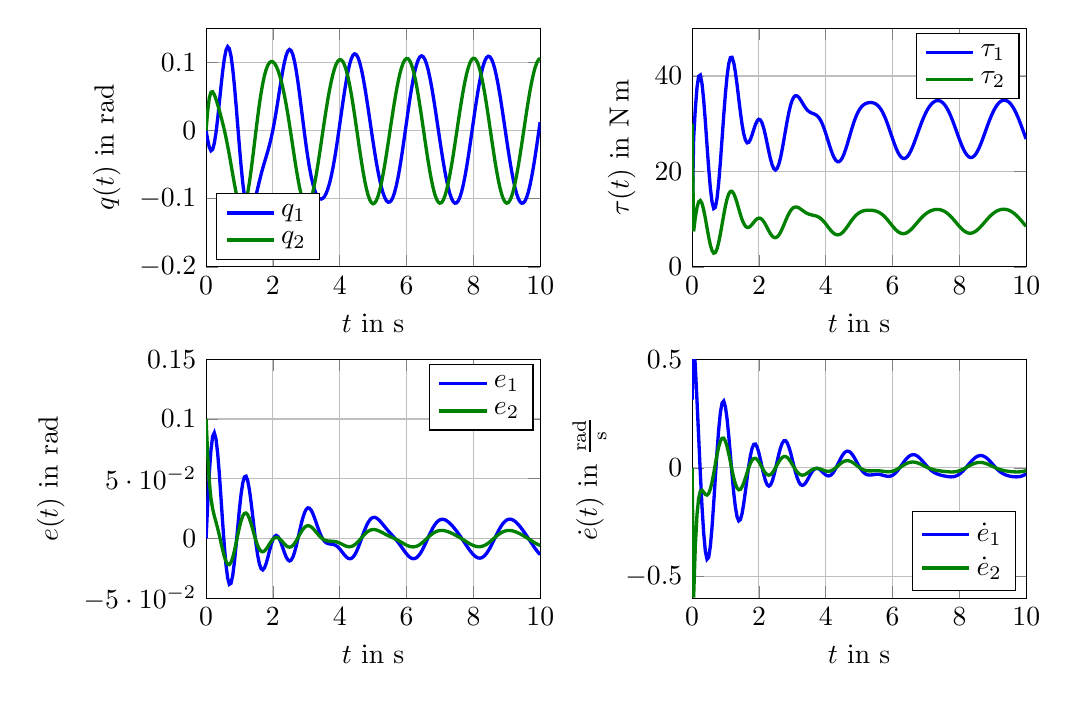
\begin{tikzpicture}

\begin{axis}[%
width=0.35\textwidth,
height=0.25\textwidth,
scale only axis,
xmin=0,
xmax=10,
xlabel={$t$ in $\mathrm{s}$},
xmajorgrids,
ymin=-0.2,
ymax=0.15,
ylabel={$q(t)$ in $\mathrm{rad}$},
ymajorgrids,
name=plot1,
legend style={at={(0.03,0.03)},anchor=south west,draw=black,fill=white,legend cell align=left}
]
\addplot [
color=blue,
solid,
line width=1.2pt
]
table[row sep=crcr]{
0 0\\
0.0461133808868633 -0.013130509080108\\
0.0961133808868633 -0.0246279295907629\\
0.146113380886863 -0.0296840597558359\\
0.196113380886863 -0.0276844734640658\\
0.246113380886863 -0.0186349741079949\\
0.296113380886864 -0.00324480847455139\\
0.346113380886864 0.0171001861611161\\
0.396113380886864 0.0404607921010105\\
0.446113380886864 0.0645398416292712\\
0.496113380886864 0.0869199184313608\\
0.546113380886864 0.105311654670631\\
0.596113380886864 0.117783052978138\\
0.646113380886864 0.122945367440964\\
0.696113380886864 0.120078073064037\\
0.746113380886864 0.109183171184207\\
0.796113380886864 0.0909665448883328\\
0.846113380886864 0.0667507713035266\\
0.896113380886864 0.0383297078996389\\
0.946113380886864 0.00778050703948682\\
0.996113380886864 -0.0227466239651492\\
1.04611338088686 -0.0512373774136238\\
1.09611338088685 -0.075996932711773\\
1.14611338088685 -0.0957872328257093\\
1.19611338088684 -0.109903805309698\\
1.24611338088684 -0.118187144781364\\
1.29611338088683 -0.12097308168019\\
1.34611338088683 -0.118994197857551\\
1.39611338088682 -0.113249058388341\\
1.44611338088682 -0.104857710666282\\
1.49611338088681 -0.0949211420600988\\
1.5461133808868 -0.0843999215325426\\
1.5961133808868 -0.0740236452767566\\
1.64611338088679 -0.0642384538790939\\
1.69611338088679 -0.0551951513642348\\
1.74611338088678 -0.0467757673040496\\
1.79611338088678 -0.0386522464627172\\
1.84611338088677 -0.0303677697830526\\
1.89611338088677 -0.0214293163470201\\
1.94611338088676 -0.011399599311528\\
1.99611338088675 2.25966098982704e-05\\
2.04611338088675 0.0129425780765532\\
2.09611338088674 0.0272363721253906\\
2.14611338088674 0.0425463749224628\\
2.19611338088673 0.0583051146998399\\
2.24611338088673 0.0737831306841329\\
2.29611338088672 0.0881545850860129\\
2.34611338088672 0.10057276834855\\
2.39611338088671 0.110247201155498\\
2.4461133808867 0.116514507661835\\
2.4961133808867 0.118896446983843\\
2.54611338088669 0.117140197291486\\
2.59611338088669 0.111237942012611\\
2.64611338088668 0.101424814332914\\
2.69611338088668 0.088156189759209\\
2.74611338088667 0.0720671064809195\\
2.79611338088667 0.0539181755058075\\
2.84611338088666 0.0345336099437566\\
2.89611338088666 0.0147377887922064\\
2.94611338088665 -0.00470311419245146\\
2.99611338088664 -0.0231285939693096\\
3.04611338088664 -0.0400160108400861\\
3.09611338088663 -0.0549952507657893\\
3.14611338088663 -0.0678459350170846\\
3.19611338088662 -0.0784794821104951\\
3.24611338088662 -0.0869100494690685\\
3.29611338088661 -0.0932193908900987\\
3.34611338088661 -0.0975208968805302\\
3.3961133808866 -0.0999276143899345\\
3.44611338088659 -0.100528033268343\\
3.49611338088659 -0.0993720766767277\\
3.54611338088658 -0.0964682383796218\\
3.59611338088658 -0.0917913483940768\\
3.64611338088657 -0.0852991694744882\\
3.69611338088657 -0.0769550483417817\\
3.74611338088656 -0.0667532492269655\\
3.79611338088656 -0.0547434238884863\\
3.84611338088655 -0.0410509176937022\\
3.89611338088655 -0.0258902264544511\\
3.94611338088654 -0.00956981378116695\\
3.99611338088653 0.00751244641577521\\
4.04611338088655 0.0248828586235484\\
4.09611338088657 0.0420132113928086\\
4.14611338088658 0.0583477340954009\\
4.1961133808866 0.0733331784102274\\
4.24611338088662 0.0864493534016629\\
4.29611338088663 0.0972375908001792\\
4.34611338088665 0.105324996103268\\
4.39611338088667 0.110442869224306\\
4.44611338088668 0.112438272462652\\
4.4961133808867 0.111278316308865\\
4.54611338088672 0.107047282779517\\
4.59611338088673 0.099937193286868\\
4.64611338088675 0.0902328493761728\\
4.69611338088677 0.0782927263514487\\
4.74611338088678 0.0645273672778066\\
4.7961133808868 0.0493770790535224\\
4.84611338088682 0.0332907362751722\\
4.89611338088683 0.0167073223023117\\
4.94611338088685 4.14736146800391e-05\\
4.99611338088687 -0.0163262282024387\\
5.04611338088688 -0.0320540879495022\\
5.0961133808869 -0.0468397420866893\\
5.14611338088692 -0.0604172356200898\\
5.19611338088693 -0.0725521048636866\\
5.24611338088695 -0.0830359787774381\\
5.29611338088697 -0.0916821246328736\\
5.34611338088698 -0.0983230806003963\\
5.396113380887 -0.102811094085549\\
5.44611338088702 -0.10502158918928\\
5.49611338088703 -0.104859389521205\\
5.54611338088705 -0.102266985610528\\
5.59611338088707 -0.0972338074330889\\
5.64611338088708 -0.0898052737724728\\
5.6961133808871 -0.0800903557326003\\
5.74611338088712 -0.0682665092680703\\
5.79611338088713 -0.0545810826335007\\
5.84611338088715 -0.039348656401233\\
5.89611338088717 -0.0229441820528047\\
5.94611338088718 -0.00579219938924608\\
5.9961133808872 0.0116472177461691\\
6.04611338088722 0.028894857203327\\
6.09611338088723 0.0454700123545806\\
6.14611338088725 0.0609082449316503\\
6.19611338088727 0.0747782189318806\\
6.24611338088728 0.0866967280554568\\
6.2961133808873 0.096341261051956\\
6.34611338088732 0.103459683768962\\
6.39611338088733 0.107876831641694\\
6.44611338088735 0.109497982612146\\
6.49611338088737 0.108309313263195\\
6.54611338088738 0.104375537701173\\
6.5961133808874 0.0978350036387332\\
6.64611338088742 0.0888925876248747\\
6.69611338088743 0.077810800077874\\
6.74611338088745 0.0648995799474569\\
6.79611338088747 0.0505053180402462\\
6.84611338088748 0.0349996803324086\\
6.8961133808875 0.0187687901742182\\
6.94611338088752 0.00220325909540118\\
6.99611338088753 -0.0143105710293264\\
7.04611338088755 -0.0303979839162961\\
7.09611338088757 -0.0457018454592961\\
7.14611338088758 -0.0598873462089273\\
7.1961133808876 -0.0726458562468541\\
7.24611338088762 -0.0836982949003417\\
7.29611338088763 -0.0927984165308053\\
7.34611338088765 -0.0997363372170145\\
7.39611338088767 -0.104342489926871\\
7.44611338088768 -0.106492020980499\\
7.4961133808877 -0.106109455837147\\
7.54611338088772 -0.103173295043122\\
7.59611338088773 -0.09772007552577\\
7.64611338088775 -0.0898473661233673\\
7.69611338088777 -0.07971516926352\\
7.74611338088778 -0.0675452741652137\\
7.7961133808878 -0.0536182428575431\\
7.84611338088782 -0.0382678922362514\\
7.89611338088783 -0.0218733402403456\\
7.94611338088785 -0.00484888543939533\\
7.99611338088787 0.0123678390533405\\
8.04611338088784 0.0293288751623915\\
8.09611338088782 0.0455894916531302\\
8.14611338088779 0.0607216607234347\\
8.19611338088776 0.0743268987602662\\
8.24611338088773 0.0860480024853263\\
8.29611338088771 0.0955793172391096\\
8.34611338088768 0.102675273706414\\
8.39611338088765 0.107157009471367\\
8.44611338088762 0.10891694772227\\
8.49611338088759 0.107921241652294\\
8.54611338088757 0.104210021189679\\
8.59611338088754 0.0978954135300816\\
8.64611338088751 0.0891573640368073\\
8.69611338088748 0.0782373669923114\\
8.74611338088746 0.0654303247810292\\
8.79611338088743 0.0510748774216052\\
8.8461133808874 0.0355426614184611\\
8.89611338088737 0.0192270429622388\\
8.94611338088735 0.00253190294031583\\
8.99611338088732 -0.0141389840610928\\
9.04611338088729 -0.0303915383238147\\
9.09611338088726 -0.0458496508539192\\
9.14611338088723 -0.0601620524884475\\
9.19611338088721 -0.0730078637438097\\
9.24611338088718 -0.08410105791181\\
9.29611338088715 -0.0931941544762603\\
9.34611338088712 -0.100081472499902\\
9.3961133808871 -0.104602216361344\\
9.44611338088707 -0.106643553225221\\
9.49611338088704 -0.106143695276373\\
9.54611338088701 -0.10309484614826\\
9.59611338088699 -0.0975457356847811\\
9.64611338088696 -0.0896033717088555\\
9.69611338088693 -0.0794335967790235\\
9.7461133808869 -0.0672600587878697\\
9.79611338088687 -0.0533612846460199\\
9.84611338088685 -0.0380656756296236\\
9.89611338088682 -0.0217444035972686\\
9.94611338088679 -0.00480235711289676\\
9.99611338088676 0.0123325573812787\\
};
\addlegendentry{$q_1$};

\addplot [
color=green!50!black,
solid,
line width=1.2pt
]
table[row sep=crcr]{
0 0\\
0.0461133808868633 0.0277893220667821\\
0.0961133808868633 0.0478611949128803\\
0.146113380886863 0.0561848539705151\\
0.196113380886863 0.0567930047172676\\
0.246113380886863 0.0527024274563873\\
0.296113380886864 0.0460104697120632\\
0.346113380886864 0.0380269238388631\\
0.396113380886864 0.0294290560405176\\
0.446113380886864 0.0204287494513818\\
0.496113380886864 0.0109404822711698\\
0.546113380886864 0.000738951678277065\\
0.596113380886864 -0.010403948770745\\
0.646113380886864 -0.022611232965033\\
0.696113380886864 -0.0358278903686522\\
0.746113380886864 -0.0497857416112706\\
0.796113380886864 -0.0640053670888828\\
0.846113380886864 -0.0778306426496549\\
0.896113380886864 -0.0904881816202592\\
0.946113380886864 -0.101162124947203\\
0.996113380886864 -0.109074579024861\\
1.04611338088686 -0.113563066159398\\
1.09611338088685 -0.114147658325481\\
1.14611338088685 -0.110581399871453\\
1.19611338088684 -0.102878468785398\\
1.24611338088684 -0.0913161872193872\\
1.29611338088683 -0.0764101129084351\\
1.34611338088683 -0.0588656316880919\\
1.39611338088682 -0.0395133590120694\\
1.44611338088682 -0.0192377803117113\\
1.49611338088681 0.00109167925206703\\
1.5461133808868 0.0206800143899431\\
1.5961133808868 0.0388519799891556\\
1.64611338088679 0.0550813191035512\\
1.69611338088679 0.0690034659634567\\
1.74611338088678 0.0804125287585372\\
1.79611338088678 0.0892444688891466\\
1.84611338088677 0.095549546161424\\
1.89611338088677 0.0994581354725434\\
1.94611338088676 0.101144629588253\\
1.99611338088675 0.100794089105703\\
2.04611338088675 0.0985755622744673\\
2.09611338088674 0.0946247549061187\\
2.14611338088674 0.0890372608317418\\
2.19611338088673 0.0818721246285841\\
2.24611338088673 0.073164278461393\\
2.29611338088672 0.0629434658906935\\
2.34611338088672 0.0512566696291293\\
2.39611338088671 0.0381908010603431\\
2.4461133808867 0.0238924830253237\\
2.4961133808867 0.00858215735076621\\
2.54611338088669 -0.00743954726276316\\
2.59611338088669 -0.0237943034542744\\
2.64611338088668 -0.0400374686275984\\
2.69611338088668 -0.0556773545129072\\
2.74611338088667 -0.070200517599644\\
2.79611338088667 -0.0831006543799507\\
2.84611338088666 -0.0939084672844351\\
2.89611338088666 -0.102219928001809\\
2.94611338088665 -0.107720615086732\\
2.99611338088664 -0.110204175452757\\
3.04611338088664 -0.109583442120546\\
3.09611338088663 -0.10589335899075\\
3.14611338088663 -0.0992856272008577\\
3.19611338088662 -0.0900158394512865\\
3.24611338088662 -0.0784246752149205\\
3.29611338088661 -0.06491532599225\\
3.34611338088661 -0.0499295795256381\\
3.3961133808866 -0.0339248799931171\\
3.44611338088659 -0.0173542589853255\\
3.49611338088659 -0.000650420178404475\\
3.54611338088658 0.0157854120959333\\
3.59611338088658 0.0315899028770628\\
3.64611338088657 0.0464398275432171\\
3.69611338088657 0.0600510493481002\\
3.74611338088656 0.0721754383249062\\
3.79611338088656 0.0825969936620644\\
3.84611338088655 0.091128350717776\\
3.89611338088655 0.097608634011804\\
3.94611338088654 0.101903294906348\\
3.99611338088653 0.103906195120446\\
4.04611338088655 0.103543815172512\\
4.09611338088657 0.100781124320856\\
4.14611338088658 0.0956283779520831\\
4.1961133808866 0.0881479301640255\\
4.24611338088662 0.0784600749458598\\
4.29611338088663 0.0667469637651054\\
4.34611338088665 0.0532537886613598\\
4.39611338088667 0.0382866565925481\\
4.44611338088668 0.0222068885112276\\
4.4961133808867 0.00542181851113431\\
4.54611338088672 -0.0116275001493687\\
4.59611338088673 -0.0284809971143437\\
4.64611338088675 -0.0446758162827393\\
4.69611338088677 -0.0597631014411935\\
4.74611338088678 -0.0733243572961591\\
4.7961133808868 -0.0849864776298554\\
4.84611338088682 -0.0944346559104246\\
4.89611338088683 -0.101422553134177\\
4.94611338088685 -0.105779283578579\\
4.99611338088687 -0.107412987611754\\
5.04611338088688 -0.106310987094022\\
5.0961133808869 -0.102536751422301\\
5.14611338088692 -0.0962241194109399\\
5.19611338088693 -0.0875693960037058\\
5.24611338088695 -0.0768220466141083\\
5.29611338088697 -0.0642747290387682\\
5.34611338088698 -0.0502533323762678\\
5.396113380887 -0.0351075493275971\\
5.44611338088702 -0.0192023196319415\\
5.49611338088703 -0.00291028032863435\\
5.54611338088705 0.0133948263139579\\
5.59611338088707 0.0293439796991349\\
5.64611338088708 0.0445782216927225\\
5.6961133808871 0.0587538147114703\\
5.74611338088712 0.071547486337623\\
5.79611338088713 0.0826619480129216\\
5.84611338088715 0.0918317619499933\\
5.89611338088717 0.0988295027725047\\
5.94611338088718 0.103472035205867\\
5.9961133808872 0.105626620418359\\
6.04611338088722 0.105216482191105\\
6.09611338088723 0.102225417874455\\
6.14611338088725 0.0967010334279264\\
6.19611338088727 0.0887562193919503\\
6.24611338088728 0.078568564417942\\
6.2961133808873 0.0663775191723005\\
6.34611338088732 0.0524792648361997\\
6.39611338088733 0.0372193913890557\\
6.44611338088735 0.0209836338043721\\
6.49611338088737 0.00418703319362316\\
6.54611338088738 -0.0127380263410851\\
6.5961133808874 -0.0293544102126953\\
6.64611338088742 -0.0452329532938865\\
6.69611338088743 -0.0599648282911906\\
6.74611338088745 -0.0731731269552634\\
6.79611338088747 -0.0845232738097224\\
6.84611338088748 -0.0937319533411069\\
6.8961133808875 -0.100574296476182\\
6.94611338088752 -0.10488914121821\\
6.99611338088753 -0.106582257286781\\
7.04611338088755 -0.105627506364413\\
7.09611338088757 -0.102065996209372\\
7.14611338088758 -0.0960033729890278\\
7.1961133808876 -0.0876054732890299\\
7.24611338088762 -0.0770926158680297\\
7.29611338088763 -0.0647328454081071\\
7.34611338088765 -0.0508344422409703\\
7.39611338088767 -0.035737984568761\\
7.44611338088768 -0.0198081994754579\\
7.4961133808877 -0.00342577619972915\\
7.54611338088772 0.0130207486461759\\
7.59611338088773 0.0291429782209679\\
7.64611338088775 0.044560495501269\\
7.69611338088777 0.0589085511008673\\
7.74611338088778 0.0718455860116093\\
7.7961133808878 0.0830605498614822\\
7.84611338088782 0.0922799354429561\\
7.89611338088783 0.0992744038866691\\
7.94611338088785 0.103864828999847\\
7.99611338088787 0.105927550738441\\
8.04611338088784 0.1053986026976\\
8.09611338088782 0.102276672084705\\
8.14611338088779 0.0966245665808191\\
8.19611338088776 0.088569002245062\\
8.24611338088773 0.0782985886244153\\
8.29611338088771 0.0660599666281089\\
8.34611338088768 0.0521521437435717\\
8.39611338088765 0.0369191604156542\\
8.44611338088762 0.0207413016935121\\
8.49611338088759 0.00402513243087863\\
8.54611338088757 -0.0128073214185334\\
8.59611338088754 -0.0293298987323058\\
8.64611338088751 -0.0451237829014752\\
8.69611338088748 -0.0597887878959155\\
8.74611338088746 -0.0729541178081967\\
8.79611338088743 -0.0842882864450781\\
8.8461133808874 -0.0935079067198411\\
8.89611338088737 -0.100385087448961\\
8.94611338088735 -0.104753210442129\\
8.99611338088732 -0.106510907012798\\
9.04611338088729 -0.105624112966538\\
9.09611338088726 -0.102126155066719\\
9.14611338088723 -0.096115906607687\\
9.19611338088721 -0.0877541378278119\\
9.24611338088718 -0.0772582684027438\\
9.29611338088715 -0.0648957934501012\\
9.34611338088712 -0.0509766926713761\\
9.3961133808871 -0.0358451401336075\\
9.44611338088707 -0.0198708109423045\\
9.49611338088704 -0.0034400370386422\\
9.54611338088701 0.0130529925310984\\
9.59611338088699 0.0292148501579062\\
9.64611338088696 0.0446612206482419\\
9.69611338088693 0.0590249330614507\\
9.7461133808869 0.0719636374726464\\
9.79611338088687 0.0831670872241474\\
9.84611338088685 0.0923639675945174\\
9.89611338088682 0.0993281811531499\\
9.94611338088679 0.103884464647415\\
9.99611338088676 0.10591317874652\\
};
\addlegendentry{$q_2$};

\end{axis}

\begin{axis}[%
width=0.35\textwidth,
height=0.25\textwidth,
scale only axis,
xmin=0,
xmax=10,
xlabel={$t$ in $\mathrm{s}$},
xmajorgrids,
ymin=-0.05,
ymax=0.15,
ylabel={$e(t)$ in $\mathrm{rad}$},
ymajorgrids,
name=plot3,
at=(plot1.below south west),
anchor=above north west,
legend style={draw=black,fill=white,legend cell align=left}
]
\addplot [
color=blue,
solid,
line width=1.2pt
]
table[row sep=crcr]{
0 0\\
0.0461133808868633 0.0275668347820642\\
0.0961133808868633 0.0543660978101026\\
0.146113380886863 0.0739918180956771\\
0.196113380886863 0.0854708178650623\\
0.246113380886863 0.0884770129891125\\
0.296113380886864 0.0834227990460991\\
0.346113380886864 0.0714395078774954\\
0.396113380886864 0.0542604642910367\\
0.446113380886864 0.0340306254220125\\
0.496113380886864 0.0130726272437322\\
0.546113380886864 -0.00635917870248194\\
0.596113380886864 -0.0223071850797095\\
0.646113380886864 -0.033297040346153\\
0.696113380886864 -0.0384647261116577\\
0.746113380886864 -0.0376143958353965\\
0.796113380886864 -0.031204601915327\\
0.846113380886864 -0.020267198080838\\
0.896113380886864 -0.006269084270145\\
0.946113380886864 0.00906772803994482\\
0.996113380886864 0.0239676110307766\\
1.04611338088686 0.036801051711669\\
1.09611338088685 0.0462587644924362\\
1.14611338088685 0.0514794744858724\\
1.19611338088684 0.052117460908707\\
1.24611338088684 0.048345105900252\\
1.29611338088683 0.0407950911086482\\
1.34611338088683 0.030454503818945\\
1.39611338088682 0.0185278019962985\\
1.44611338088682 0.00628724361500137\\
1.49611338088681 -0.00507140361499402\\
1.5461133808868 -0.0145525544356088\\
1.5961133808868 -0.0214522226216784\\
1.64611338088679 -0.025409873215727\\
1.69611338088679 -0.0264181955881581\\
1.74611338088678 -0.0247930080447785\\
1.79611338088678 -0.0211096965103106\\
1.84611338088677 -0.0161158034396618\\
1.89611338088677 -0.0106313072825032\\
1.94611338088676 -0.0054486357679359\\
1.99611338088675 -0.0012435836755601\\
2.04611338088675 0.00149374762536742\\
2.09611338088674 0.00250179609391312\\
2.14611338088674 0.001761383417343\\
2.19611338088673 -0.00051877029887698\\
2.24611338088673 -0.00394109180304597\\
2.29611338088672 -0.00797659451449191\\
2.34611338088672 -0.0120330743099599\\
2.39611338088671 -0.0155259447634665\\
2.4461133808867 -0.0179440406105599\\
2.4961133808867 -0.0189039013087501\\
2.54611338088669 -0.0181877213233292\\
2.59611338088669 -0.0157620741141653\\
2.64611338088668 -0.0117764872380782\\
2.69611338088668 -0.00654284280679605\\
2.74611338088667 -0.000498331132067265\\
2.79611338088667 0.00584376746724801\\
2.84611338088666 0.0119499632789884\\
2.89611338088666 0.0173228348373497\\
2.94611338088665 0.0215513492719495\\
2.99611338088664 0.024349581035006\\
3.04611338088664 0.0255796851381997\\
3.09611338088663 0.0252570825465187\\
3.14611338088663 0.0235381766773098\\
3.19611338088662 0.0206931377095604\\
3.24611338088662 0.0170680105880064\\
3.29611338088661 0.0130414003185984\\
3.34611338088661 0.00898120284195636\\
3.3961133808866 0.00520635799791389\\
3.44611338088659 0.00195756621707305\\
3.49611338088659 -0.000620468998364335\\
3.54611338088658 -0.00248423758853959\\
3.59611338088658 -0.00368451950437876\\
3.64611338088657 -0.00434915762036331\\
3.69611338088657 -0.00465829861065126\\
3.74611338088656 -0.00481552612191098\\
3.79611338088656 -0.00501851908459702\\
3.84611338088655 -0.00543265552907354\\
3.89611338088655 -0.00617039717513766\\
3.94611338088654 -0.00727842129836523\\
3.99611338088653 -0.00873343348150625\\
4.04611338088655 -0.0104465329216899\\
4.09611338088657 -0.0122750431735582\\
4.14611338088658 -0.0140399757556389\\
4.1961133808866 -0.0155468340092987\\
4.24611338088662 -0.0166073145206011\\
4.29611338088663 -0.0170596002286749\\
4.34611338088665 -0.0167853020646883\\
4.39611338088667 -0.0157216128322785\\
4.44611338088668 -0.0138678054113782\\
4.4961133808867 -0.0112857706337726\\
4.54611338088672 -0.00809480681136196\\
4.59611338088673 -0.00446132538842683\\
4.64611338088675 -0.00058452228134584\\
4.69611338088677 0.00332062060094815\\
4.74611338088678 0.00704140807102134\\
4.7961133808868 0.0103848639194997\\
4.84611338088682 0.0131928369475298\\
4.89611338088683 0.0153533013271914\\
4.94611338088685 0.016806761464756\\
4.99611338088687 0.0175472152680653\\
5.04611338088688 0.0176177622475398\\
5.0961133808869 0.0171015738673388\\
5.14611338088692 0.0161094772802336\\
5.19611338088693 0.0147657604626724\\
5.24611338088695 0.013193939896301\\
5.29611338088697 0.0115041340613067\\
5.34611338088698 0.00978338656176733\\
5.396113380887 0.00808983769348845\\
5.44611338088702 0.0064511221379879\\
5.49611338088703 0.00486684384611143\\
5.54611338088705 0.00331450964238801\\
5.59611338088707 0.0017579395346789\\
5.64611338088708 0.000156946677692379\\
5.6961133808871 -0.00152299121973606\\
5.74611338088712 -0.00330226608068429\\
5.79611338088713 -0.00518086033943704\\
5.84611338088715 -0.00713491682137598\\
5.89611338088717 -0.00911644157659895\\
5.94611338088718 -0.0110560356900867\\
5.9961133808872 -0.0128682048116907\\
6.04611338088722 -0.014458531501261\\
6.09611338088723 -0.0157318441351297\\
6.14611338088725 -0.0166004865917002\\
6.19611338088727 -0.0169918745307806\\
6.24611338088728 -0.0168546891742448\\
6.2961133808873 -0.0161632704803262\\
6.34611338088732 -0.0149199897302843\\
6.39611338088733 -0.0131555752495993\\
6.44611338088735 -0.0109275155608366\\
6.49611338088737 -0.00831676758809956\\
6.54611338088738 -0.00542306173304838\\
6.5961133808874 -0.00235913574035442\\
6.64611338088742 0.000755739469859296\\
6.69611338088743 0.00380254687440161\\
6.74611338088745 0.00666919540122453\\
6.79611338088747 0.00925662493260754\\
6.84611338088748 0.0114838928901076\\
6.8961133808875 0.0132918334550863\\
6.94611338088752 0.0146449759838283\\
6.99611338088753 0.0155315580947433\\
7.04611338088755 0.0159616582141264\\
7.09611338088757 0.0159636772397452\\
7.14611338088758 0.0155795878688833\\
7.1961133808876 0.0148595118456685\\
7.24611338088762 0.0138562560190547\\
7.29611338088763 0.0126204259591129\\
7.34611338088765 0.0111966431782879\\
7.39611338088767 0.00962123353474283\\
7.44611338088768 0.00792155392917228\\
7.4961133808877 0.00611691016205054\\
7.54611338088772 0.00422081907501215\\
7.59611338088773 0.00224420762742246\\
7.64611338088775 0.000199039028679918\\
7.69611338088777 -0.00189817768869505\\
7.74611338088778 -0.00402350118339427\\
7.7961133808878 -0.00614370011522662\\
7.84611338088782 -0.00821568098617177\\
7.89611338088783 -0.0101872833888596\\
7.94611338088785 -0.0119993496397305\\
7.99611338088787 -0.0135888261186526\\
8.04611338088784 -0.0148925494601303\\
8.09611338088782 -0.0158513234335047\\
8.14611338088779 -0.0164139023833331\\
8.19611338088776 -0.0165405543590397\\
8.24611338088773 -0.0162059636040131\\
8.29611338088771 -0.0154013266674038\\
8.34611338088768 -0.0141355796676836\\
8.39611338088765 -0.012435753079241\\
8.44611338088762 -0.0103464806709461\\
8.49611338088759 -0.00792869597719838\\
8.54611338088757 -0.0052575452215618\\
8.59611338088754 -0.0024195456317157\\
8.64611338088751 0.000490963057913504\\
8.69611338088748 0.0033759799599551\\
8.74611338088746 0.006138450567651\\
8.79611338088743 0.00868706555125856\\
8.8461133808874 0.0109409118040781\\
8.89611338088737 0.0128335806671037\\
8.94611338088735 0.0143163321389669\\
8.99611338088732 0.0153599711265779\\
9.04611338088729 0.0159552126217258\\
9.09611338088726 0.0161114826344599\\
9.14611338088723 0.0158542941485019\\
9.19611338088721 0.0152215193427253\\
9.24611338088718 0.0142590190306217\\
9.29611338088715 0.0130161639046586\\
9.34611338088712 0.011541778461253\\
9.3961133808871 0.00988095996927317\\
9.44611338088707 0.00807308617392608\\
9.49611338088704 0.00615114960127956\\
9.54611338088701 0.00414237018011827\\
9.59611338088699 0.00206986778636344\\
9.64611338088696 -4.49553859426244e-05\\
9.69611338088693 -0.00217975017334363\\
9.7461133808869 -0.00430871656093214\\
9.79611338088687 -0.00640065832698345\\
9.84611338088685 -0.00841789759307005\\
9.89611338088682 -0.0103162200322387\\
9.94611338088679 -0.0120458779665576\\
9.99611338088676 -0.0135535444469379\\
};
\addlegendentry{$e_1$};

\addplot [
color=green!50!black,
solid,
line width=1.2pt
]
table[row sep=crcr]{
0 0.1\\
0.0461133808868633 0.0711631539013666\\
0.0961133808868633 0.0476146729855486\\
0.146113380886863 0.033463473124296\\
0.196113380886863 0.0248203422351115\\
0.246113380886863 0.0188663478924229\\
0.296113380886864 0.0137514732609427\\
0.346113380886864 0.00845664938382557\\
0.396113380886864 0.0026315675889764\\
0.446113380886864 -0.00358051437195007\\
0.496113380886864 -0.00971949520554234\\
0.546113380886864 -0.0151752773802334\\
0.596113380886864 -0.0193342194485949\\
0.646113380886864 -0.0216965253748082\\
0.696113380886864 -0.0219584540323445\\
0.746113380886864 -0.0200562972698471\\
0.796113380886864 -0.016172623482665\\
0.846113380886864 -0.0107090513889567\\
0.896113380886864 -0.00423307477178803\\
0.946113380886864 0.00259165789591931\\
0.996113380886864 0.00908203334976807\\
1.04611338088686 0.014610590191249\\
1.09611338088685 0.0186717904270513\\
1.14611338088685 0.0209330727766399\\
1.19611338088684 0.0212651218330146\\
1.24611338088684 0.0197474118705713\\
1.29611338088683 0.0166481699354212\\
1.34611338088683 0.0123820584653928\\
1.39611338088682 0.00745273538256257\\
1.44611338088682 0.0023895452322645\\
1.49611338088681 -0.00231266631771153\\
1.5461133808868 -0.00624368868800533\\
1.5961133808868 -0.00911381176983541\\
1.64611338088679 -0.0107735607637298\\
1.69611338088679 -0.0112171215624796\\
1.74611338088678 -0.0105704898774379\\
1.79611338088678 -0.00906647831761523\\
1.84611338088677 -0.007009852122826\\
1.89611338088677 -0.00473687908050617\\
1.94611338088676 -0.00257416253697498\\
1.99611338088675 -0.000801543430610063\\
2.04611338088675 0.000376913693686545\\
2.09611338088674 0.000851112992321448\\
2.14611338088674 0.000611066263086699\\
2.19611338088673 -0.000258777676181113\\
2.24611338088673 -0.00159550311255283\\
2.29611338088672 -0.00318152291765181\\
2.34611338088672 -0.00477309640639958\\
2.39611338088671 -0.00613017743080342\\
2.4461133808867 -0.00704424794584275\\
2.4961133808867 -0.00736117028508715\\
2.54611338088669 -0.00699677843914033\\
2.59611338088669 -0.00594386476501286\\
2.64611338088668 -0.004270289712192\\
2.69611338088668 -0.00210898988804151\\
2.74611338088667 0.000358478718569477\\
2.79611338088667 0.00292266380844003\\
2.84611338088666 0.00536877324585311\\
2.89611338088666 0.00749867160978289\\
2.94611338088665 0.00915014803545977\\
2.99611338088664 0.0102116297776645\\
3.04611338088664 0.0106309661523871\\
3.09611338088663 0.0104174910922992\\
3.14611338088663 0.00963730010601382\\
3.19611338088662 0.00840249249886352\\
3.24611338088662 0.00685589986605624\\
3.29611338088661 0.00515338301918045\\
3.34611338088661 0.00344600630287771\\
3.3961133808866 0.00186425636354468\\
3.44611338088659 0.000506023905810515\\
3.49611338088659 -0.000570566887309325\\
3.54611338088658 -0.00134908639406411\\
3.59611338088658 -0.00185173465780861\\
3.64611338088657 -0.00213206920345774\\
3.69611338088657 -0.0022647049471796\\
3.74611338088656 -0.00233339944385655\\
3.79611338088656 -0.00241900309057437\\
3.84611338088655 -0.00258865667921014\\
3.89611338088655 -0.0028873776197889\\
3.94611338088654 -0.00333282785508138\\
3.99611338088653 -0.00391364944535405\\
4.04611338088655 -0.0045913392043487\\
4.09611338088657 -0.00530525642239957\\
4.14611338088658 -0.00598005085723292\\
4.1961133808866 -0.00653458321159832\\
4.24611338088662 -0.00689129959699522\\
4.29611338088663 -0.00698502079204126\\
4.34611338088665 -0.00677021543861144\\
4.39611338088667 -0.00622603296299522\\
4.44611338088668 -0.00535865343173968\\
4.4961133808867 -0.00420083144545513\\
4.54611338088672 -0.00280882555254162\\
4.59611338088673 -0.0012571711049567\\
4.64611338088675 0.000368057942930253\\
4.69611338088677 0.00197675704022197\\
4.74611338088678 0.00348231841505976\\
4.7961133808868 0.00480848705831981\\
4.84611338088682 0.00589496187182004\\
4.89611338088683 0.00670129674213316\\
4.94611338088685 0.0072088165272957\\
4.99611338088687 0.00742044193666079\\
5.04611338088688 0.00735851112587406\\
5.0961133808869 0.00706088352387522\\
5.14611338088692 0.00657579231613624\\
5.19611338088693 0.00595604905133915\\
5.24611338088695 0.00525327126531708\\
5.29611338088697 0.00451278606578815\\
5.34611338088698 0.00376975915361241\\
5.396113380887 0.00304692569814343\\
5.44611338088702 0.00235408455255708\\
5.49611338088703 0.00168929326305996\\
5.54611338088705 0.0010414993880563\\
5.59611338088707 0.000394188520265577\\
5.64611338088708 -0.000270463352819376\\
5.6961133808871 -0.000967470310413318\\
5.74611338088712 -0.00170544745644845\\
5.79611338088713 -0.00248395744132318\\
5.84611338088715 -0.00329206791134\\
5.89611338088717 -0.00410824638042698\\
5.94611338088718 -0.00490156815456651\\
5.9961133808872 -0.00563407474326456\\
6.04611338088722 -0.0062640062229723\\
6.09611338088723 -0.00674954997606086\\
6.14611338088725 -0.00705270633316912\\
6.19611338088727 -0.00714287243964443\\
6.24611338088728 -0.00699978906922401\\
6.2961133808873 -0.00661557619940477\\
6.34611338088732 -0.0059956916136371\\
6.39611338088733 -0.00515876775970162\\
6.44611338088735 -0.00413539872509099\\
6.49611338088737 -0.00296604612815391\\
6.54611338088738 -0.00169829936103283\\
6.5961133808874 -0.000383758006805582\\
6.64611338088742 0.000925194953889451\\
6.69611338088743 0.00217848389004775\\
6.74611338088745 0.00333108807401393\\
6.79611338088747 0.00434528323806131\\
6.84611338088748 0.00519225930240487\\
6.8961133808875 0.0058530400840706\\
6.94611338088752 0.00631867416689173\\
6.99611338088753 0.00658971161168488\\
7.04611338088755 0.00667503039629526\\
7.09611338088757 0.00659012831100911\\
7.14611338088758 0.006355045894317\\
7.1961133808876 0.00599212633678459\\
7.24611338088762 0.00552384051938484\\
7.29611338088763 0.00497090243529532\\
7.34611338088765 0.00435086901850074\\
7.39611338088767 0.00367736093950616\\
7.44611338088768 0.00295996439628046\\
7.4961133808877 0.00220478913436469\\
7.54611338088772 0.00141557705604604\\
7.59611338088773 0.000595189998632981\\
7.64611338088775 -0.00025273716117765\\
7.69611338088777 -0.00112220669963893\\
7.74611338088778 -0.0020035471302845\\
7.7961133808878 -0.00288255928975845\\
7.84611338088782 -0.00374024140420519\\
7.89611338088783 -0.00455314749452415\\
7.94611338088785 -0.00529436194851111\\
7.99611338088787 -0.00593500506334407\\
8.04611338088784 -0.00644612672949589\\
8.09611338088782 -0.00680080418636458\\
8.14611338088779 -0.00697623948613676\\
8.19611338088776 -0.00695565529284564\\
8.24611338088773 -0.00672981327579596\\
8.29611338088771 -0.00629802365531504\\
8.34611338088768 -0.00566857052110936\\
8.39611338088765 -0.00485853678639405\\
8.44611338088762 -0.00389306661431536\\
8.49611338088759 -0.00280414536548076\\
8.54611338088757 -0.00162900428364141\\
8.59611338088754 -0.000408269487236441\\
8.64611338088751 0.000816024561451384\\
8.69611338088748 0.00200244349475997\\
8.74611338088746 0.00311207892694598\\
8.79611338088743 0.00411029587342447\\
8.8461133808874 0.00496821268115112\\
8.89611338088737 0.00566383105686255\\
8.94611338088735 0.00618274339082027\\
8.99611338088732 0.00651836133770317\\
9.04611338088729 0.00667163699840884\\
9.09611338088726 0.00665028716832762\\
9.14611338088723 0.00646757951292753\\
9.19611338088721 0.00614079087549495\\
9.24611338088718 0.00568949305400265\\
9.29611338088715 0.00513385047716784\\
9.34611338088712 0.00449311944875962\\
9.3961133808871 0.00378451650418236\\
9.44611338088707 0.00302257586293577\\
9.49611338088704 0.00221904997307024\\
9.54611338088701 0.00138333317090411\\
9.59611338088699 0.000523318061469786\\
9.64611338088696 -0.000353462308374505\\
9.69611338088693 -0.00123858866043725\\
9.7461133808869 -0.00212159859152021\\
9.79611338088687 -0.00298909665259779\\
9.84611338088685 -0.00382427355590853\\
9.89611338088682 -0.0046069247611073\\
9.94611338088679 -0.005313997596135\\
9.99611338088676 -0.00592063307142765\\
};
\addlegendentry{$e_2$};

\end{axis}

\begin{axis}[%
width=0.35\textwidth,
height=0.25\textwidth,
scale only axis,
xmin=0,
xmax=10,
xlabel={$t$ in $\mathrm{s}$},
xmajorgrids,
ymin=-0.6,
ymax=0.5,
ylabel={$\dot{e}(t)$ in $\mathrm{\frac{rad}{s}}$},
ymajorgrids,
name=plot2,
at=(plot3.right of south east),
anchor=left of south west,
legend style={at={(0.97,0.03)},anchor=south east,draw=black,fill=white,legend cell align=left}
]
\addplot [
color=blue,
solid,
line width=1.2pt
]
table[row sep=crcr]{
0 0.314159265358979\\
0.0461133808868633 0.59838291811541\\
0.0961133808868633 0.467940959689563\\
0.146113380886863 0.312617834909413\\
0.196113380886863 0.143828103033387\\
0.246113380886863 -0.0241917596626396\\
0.296113380886864 -0.176506723419949\\
0.346113380886864 -0.299613641994504\\
0.396113380886864 -0.383175499237131\\
0.446113380886864 -0.421204348483682\\
0.496113380886864 -0.412616465726744\\
0.546113380886864 -0.361164871542855\\
0.596113380886864 -0.274823992369767\\
0.646113380886864 -0.164750671437361\\
0.696113380886864 -0.0439716891736688\\
0.746113380886864 0.0740484420242665\\
0.796113380886864 0.176817681262662\\
0.846113380886864 0.254079912912669\\
0.896113380886864 0.298820284782734\\
0.946113380886864 0.307911554498438\\
0.996113380886864 0.282319289246062\\
1.04611338088686 0.226824243318166\\
1.09611338088685 0.149285998785654\\
1.14611338088685 0.0595495745904714\\
1.19611338088684 -0.0318392128671397\\
1.24611338088684 -0.11491657488534\\
1.29611338088683 -0.181405958557842\\
1.34611338088683 -0.22552057907031\\
1.39611338088682 -0.244401024458676\\
1.44611338088682 -0.238181795510257\\
1.49611338088681 -0.209721929077475\\
1.5461133808868 -0.164062613568055\\
1.5961133808868 -0.107693245300658\\
1.64611338088679 -0.047718854316466\\
1.69611338088679 0.00897452630639065\\
1.74611338088678 0.0564657537315615\\
1.79611338088678 0.0903803694853193\\
1.84611338088677 0.108256167402498\\
1.89611338088677 0.109668137014458\\
1.94611338088676 0.0961169053264355\\
1.99611338088675 0.0707108031182283\\
2.04611338088675 0.0376925281211534\\
2.09611338088674 0.00187510684587783\\
2.14611338088674 -0.031942753243749\\
2.19611338088673 -0.0595150537802492\\
2.24611338088673 -0.0775847354505514\\
2.29611338088672 -0.0841785597143985\\
2.34611338088672 -0.0787411389204007\\
2.39611338088671 -0.0621082439323232\\
2.4461133808867 -0.0363364301973349\\
2.4961133808867 -0.00441841930252044\\
2.54611338088669 0.0300790521312363\\
2.59611338088669 0.0634154758031062\\
2.64611338088668 0.0920759374367548\\
2.69611338088668 0.113132916509203\\
2.74611338088667 0.124537255989282\\
2.79611338088667 0.125310025765997\\
2.84611338088666 0.115614740428277\\
2.89611338088666 0.0967008846023004\\
2.94611338088665 0.0707247005140252\\
2.99611338088664 0.0404696635869648\\
3.04611338088664 0.00900359070767998\\
3.09611338088663 -0.0206816793485068\\
3.14611338088663 -0.0460009116536163\\
3.19611338088662 -0.0650360385357915\\
3.24611338088662 -0.0766990216723203\\
3.29611338088661 -0.0807849464237663\\
3.34611338088661 -0.077918560017393\\
3.3961133808866 -0.069410156266352\\
3.44611338088659 -0.0570456310314579\\
3.49611338088659 -0.0428404076033171\\
3.54611338088658 -0.0287880150163616\\
3.59611338088658 -0.0166318868034744\\
3.64611338088657 -0.00768402539537263\\
3.69611338088657 -0.00270722272852811\\
3.74611338088656 -0.00186931403088392\\
3.79611338088656 -0.00476933652927192\\
3.84611338088655 -0.0105273817722514\\
3.89611338088655 -0.0179232446180106\\
3.94611338088654 -0.0255644136831112\\
3.99611338088653 -0.0320619933823139\\
4.04611338088655 -0.0361939306582007\\
4.09611338088657 -0.0370381876424293\\
4.14611338088658 -0.0340636372557291\\
4.1961133808866 -0.0271725778099581\\
4.24611338088662 -0.016694879962029\\
4.29611338088663 -0.0033390090289557\\
4.34611338088665 0.0118910974955415\\
4.39611338088667 0.0278022896779033\\
4.44611338088668 0.0431301051905417\\
4.4961133808867 0.0566574182958325\\
4.54611338088672 0.0673241220656465\\
4.59611338088673 0.0743194681831982\\
4.64611338088675 0.0771500426330336\\
4.69611338088677 0.0756778461326683\\
4.74611338088678 0.0701248618397083\\
4.7961133808868 0.061043086653733\\
4.84611338088682 0.0492523073998826\\
4.89611338088683 0.035751613013244\\
4.94611338088685 0.0216141344912476\\
4.99611338088687 0.00787704252249699\\
5.04611338088688 -0.00456024047637543\\
5.0961133808869 -0.0150176646977799\\
5.14611338088692 -0.0230868922909085\\
5.19611338088693 -0.028649363793907\\
5.24611338088695 -0.0318597846369594\\
5.29611338088697 -0.033099159148673\\
5.34611338088698 -0.0329050377289073\\
5.396113380887 -0.0318888821514059\\
5.44611338088702 -0.0306512557928636\\
5.49611338088703 -0.0297049906837019\\
5.54611338088705 -0.0294148003096213\\
5.59611338088707 -0.0299593047787724\\
5.64611338088708 -0.0313184532647\\
5.6961133808871 -0.0332862106729387\\
5.74611338088712 -0.0355054526876031\\
5.79611338088713 -0.0375195926972284\\
5.84611338088715 -0.038833808031885\\
5.89611338088717 -0.0389780284958359\\
5.94611338088718 -0.0375641718972106\\
5.9961133808872 -0.0343313905663651\\
6.04611338088722 -0.0291751097507174\\
6.09611338088723 -0.0221580482669083\\
6.14611338088725 -0.0135038059389462\\
6.19611338088727 -0.00357559538820063\\
6.24611338088728 0.00715599127805189\\
6.2961133808873 0.0181517710284101\\
6.34611338088732 0.0288451121975772\\
6.39611338088733 0.0386819527452843\\
6.44611338088735 0.0471571673554597\\
6.49611338088737 0.0538456529517979\\
6.54611338088738 0.0584271460349223\\
6.5961133808874 0.0607041038799885\\
6.64611338088742 0.0606120353493313\\
6.69611338088743 0.0582216169929869\\
6.74611338088745 0.053731978750956\\
6.79611338088747 0.0474548639784546\\
6.84611338088748 0.0397900413427682\\
6.8961133808875 0.031193323303368\\
6.94611338088752 0.0221396535058888\\
6.99611338088753 0.0130847077127224\\
7.04611338088755 0.00442904503054004\\
7.09611338088757 -0.00351114694067073\\
7.14611338088758 -0.0105233147321017\\
7.1961133808876 -0.016505627976222\\
7.24611338088762 -0.0214612974920635\\
7.29611338088763 -0.0254812044910676\\
7.34611338088765 -0.0287174228966792\\
7.39611338088767 -0.031351316682096\\
7.44611338088768 -0.0335604585938367\\
7.4961133808877 -0.0354886025389463\\
7.54611338088772 -0.037222387034024\\
7.59611338088773 -0.0387774507356608\\
7.64611338088775 -0.0400953449490071\\
7.69611338088777 -0.041051200843433\\
7.74611338088778 -0.0414707329320688\\
7.7961133808878 -0.0411540148066447\\
7.84611338088782 -0.039902704259968\\
7.89611338088783 -0.0375471296463668\\
7.94611338088785 -0.0339699104001167\\
7.99611338088787 -0.0291235154990411\\
8.04611338088784 -0.0230402212647345\\
8.09611338088782 -0.0158341093725644\\
8.14611338088779 -0.0076958236931054\\
8.19611338088776 0.00111841098115295\\
8.24611338088773 0.0103016294831116\\
8.29611338088771 0.0195129942760698\\
8.34611338088768 0.0283952431790421\\
8.39611338088765 0.0365918307568497\\
8.44611338088762 0.0437634266873448\\
8.49611338088759 0.0496037997659669\\
8.54611338088757 0.0538551867371705\\
8.59611338088754 0.0563229988909661\\
8.64611338088751 0.0568892310297196\\
8.69611338088748 0.0555233639636014\\
8.74611338088746 0.0522890968442457\\
8.79611338088743 0.0473451082874839\\
8.8461133808874 0.0409383620476597\\
8.89611338088737 0.0333892701938293\\
8.94611338088735 0.0250691973076012\\
8.99611338088732 0.0163721075067519\\
9.04611338088729 0.00768333014875505\\
9.09611338088726 -0.000650831505010663\\
9.14611338088723 -0.0083487951478925\\
9.19611338088721 -0.0152113878844932\\
9.24611338088718 -0.0211293379762486\\
9.29611338088715 -0.026079859718759\\
9.34611338088712 -0.0301131874616472\\
9.3961133808871 -0.0333312990779086\\
9.44611338088707 -0.0358620623761193\\
9.49611338088704 -0.0378325174513991\\
9.54611338088701 -0.0393449422462738\\
9.59611338088699 -0.0404587854011176\\
9.64611338088696 -0.0411805982335029\\
9.69611338088693 -0.0414629061963301\\
9.7461133808869 -0.041211702455974\\
9.79611338088687 -0.0403010999183399\\
9.84611338088685 -0.0385928040026697\\
9.89611338088682 -0.0359575869955009\\
9.94611338088679 -0.032295912840935\\
9.99611338088676 -0.0275552573990755\\
};
\addlegendentry{$\dot{e}_1$};

\addplot [
color=green!50!black,
solid,
line width=1.2pt
]
table[row sep=crcr]{
0 -0\\
0.0461133808868633 -0.597709557817486\\
0.0961133808868633 -0.363669498194279\\
0.146113380886863 -0.218209562807172\\
0.196113380886863 -0.139540154635783\\
0.246113380886863 -0.107120280572927\\
0.296113380886864 -0.102856295717221\\
0.346113380886864 -0.11169335538529\\
0.396113380886864 -0.121988951553997\\
0.446113380886864 -0.125658680766376\\
0.496113380886864 -0.118091369783371\\
0.546113380886864 -0.0978415535143736\\
0.596113380886864 -0.0661271999837379\\
0.646113380886864 -0.0261777391205921\\
0.696113380886864 0.0175112486519833\\
0.746113380886864 0.0599503587897803\\
0.796113380886864 0.0963808591090456\\
0.846113380886864 0.12287804777141\\
0.896113380886864 0.136779658453995\\
0.946113380886864 0.136919053551903\\
0.996113380886864 0.123674759055324\\
1.04611338088686 0.0988625641091774\\
1.09611338088685 0.0654925542138588\\
1.14611338088685 0.0274056895942529\\
1.19611338088684 -0.0111890246679077\\
1.24611338088684 -0.0462303920479497\\
1.29611338088683 -0.0742981744879836\\
1.34611338088683 -0.0929979321671949\\
1.39611338088682 -0.101174093841842\\
1.44611338088682 -0.0989329673653561\\
1.49611338088681 -0.0875023775485472\\
1.5461133808868 -0.0689797014656949\\
1.5961133808868 -0.0460212701079046\\
1.64611338088679 -0.0215135496261372\\
1.69611338088679 0.00174622354789544\\
1.74611338088678 0.0213378292037892\\
1.79611338088678 0.0354518447880407\\
1.84611338088677 0.0430469788117928\\
1.89611338088677 0.0439139292289077\\
1.94611338088676 0.0386402957455883\\
1.99611338088675 0.02848540638736\\
2.04611338088675 0.0151863936584585\\
2.09611338088674 0.000724311621877888\\
2.14611338088674 -0.0129191408678562\\
2.19611338088673 -0.0239864321370589\\
2.24611338088673 -0.0311280542398804\\
2.29611338088672 -0.0335294525642007\\
2.34611338088672 -0.0309718574742293\\
2.39611338088671 -0.023824614485211\\
2.4461133808867 -0.0129733016517382\\
2.4961133808867 0.000305592051554449\\
2.54611338088669 0.0145069061565294\\
2.59611338088669 0.0280754179423663\\
2.64611338088668 0.0395790583440399\\
2.69611338088668 0.0478571431978157\\
2.74611338088667 0.0521291360765943\\
2.79611338088667 0.0520560408351471\\
2.84611338088666 0.0477527504831319\\
2.89611338088666 0.039754284593843\\
2.94611338088665 0.0289417265185599\\
2.99611338088664 0.0164357407521871\\
3.04611338088664 0.00346790362042612\\
3.09611338088663 -0.00875699032812505\\
3.14611338088663 -0.0191918922923129\\
3.19611338088662 -0.0270553425231764\\
3.24611338088662 -0.0319023496363403\\
3.29611338088661 -0.0336501378679468\\
3.34611338088661 -0.0325579712139097\\
3.3961133808866 -0.0291672962553053\\
3.44611338088659 -0.0242134749122518\\
3.49611338088659 -0.0185227405057758\\
3.54611338088658 -0.0129079888711275\\
3.59611338088658 -0.00807535850475816\\
3.64611338088657 -0.00455097228474999\\
3.69611338088657 -0.00263415388611177\\
3.74611338088656 -0.00238012689897474\\
3.79611338088656 -0.0036118478440065\\
3.84611338088655 -0.00595749174597093\\
3.89611338088655 -0.00890754664574031\\
3.94611338088654 -0.0118837883518996\\
3.99611338088653 -0.0143117519710842\\
4.04611338088655 -0.0156886475471564\\
4.09611338088657 -0.0156397871308561\\
4.14611338088658 -0.0139582507792418\\
4.1961133808866 -0.0106245056542456\\
4.24611338088662 -0.00580485569498868\\
4.29611338088663 0.000170183297959481\\
4.34611338088665 0.00684437588862413\\
4.39611338088667 0.0136861421839491\\
4.44611338088668 0.0201446611014545\\
4.4961133808867 0.0257052048835104\\
4.54611338088672 0.0299377650486833\\
4.59611338088673 0.0325343504558356\\
4.64611338088675 0.0333321097794257\\
4.69611338088677 0.0323212691738762\\
4.74611338088678 0.0296384575996997\\
4.7961133808868 0.0255471537999193\\
4.84611338088682 0.0204077500752441\\
4.89611338088683 0.0146402312709003\\
4.94611338088685 0.008682865859943\\
4.99611338088687 0.00295065691172092\\
5.04611338088688 -0.00220248023309644\\
5.0961133808869 -0.00651394485767798\\
5.14611338088692 -0.0098318090082764\\
5.19611338088693 -0.0121211874905826\\
5.24611338088695 -0.0134570954975543\\
5.29611338088697 -0.0140050345142879\\
5.34611338088698 -0.0139921466889988\\
5.396113380887 -0.01367292082349\\
5.44611338088702 -0.0132939474688878\\
5.49611338088703 -0.013062075446616\\
5.54611338088705 -0.0131196052579938\\
5.59611338088707 -0.0135290298731002\\
5.64611338088708 -0.0142684971262418\\
5.6961133808871 -0.0152378169242935\\
5.74611338088712 -0.0162736415313801\\
5.79611338088713 -0.0171715338714113\\
5.84611338088715 -0.0177120749499187\\
5.89611338088717 -0.0176879564277104\\
5.94611338088718 -0.0169291216129093\\
5.9961133808872 -0.0153233978371882\\
6.04611338088722 -0.0128306439517095\\
6.09611338088723 -0.00948916601717713\\
6.14611338088725 -0.00541398322648698\\
6.19611338088727 -0.000787393858091484\\
6.24611338088728 0.00415688754281934\\
6.2961133808873 0.00915408184008981\\
6.34611338088732 0.0139308348463849\\
6.39611338088733 0.0182274103114205\\
6.44611338088735 0.0218174027735746\\
6.49611338088737 0.024523306521529\\
6.54611338088738 0.0262269456204356\\
6.5961133808874 0.026874448192296\\
6.64611338088742 0.0264760170740674\\
6.69611338088743 0.0251011394761933\\
6.74611338088745 0.022870081112534\\
6.79611338088747 0.0199425672043513\\
6.84611338088748 0.0165045340214891\\
6.8961133808875 0.0127538111349635\\
6.94611338088752 0.00888561259527191\\
6.99611338088753 0.00507878037638737\\
7.04611338088755 0.00148379848605162\\
7.09611338088757 -0.00178638507573384\\
7.14611338088758 -0.00466179831727911\\
7.1961133808876 -0.00711649329988237\\
7.24611338088762 -0.00916498986542996\\
7.29611338088763 -0.0108544528916804\\
7.34611338088765 -0.0122535040660582\\
7.39611338088767 -0.013439037083394\\
7.44611338088768 -0.0144826867433452\\
7.4961133808877 -0.0154386459651898\\
7.54611338088772 -0.0163343273171258\\
7.59611338088773 -0.0171649688611745\\
7.64611338088775 -0.0178927599338115\\
7.69611338088777 -0.0184504948323272\\
7.74611338088778 -0.0187492296734099\\
7.7961133808878 -0.0186889805544243\\
7.84611338088782 -0.018171197315105\\
7.89611338088783 -0.0171115933071129\\
7.94611338088785 -0.0154519091865582\\
7.99611338088787 -0.0131693304624004\\
8.04611338088784 -0.0102825505900395\\
8.09611338088782 -0.0068538513285382\\
8.14611338088779 -0.00298702374976631\\
8.19611338088776 0.00117857594705717\\
8.24611338088773 0.00547711699336989\\
8.29611338088771 0.00972749911216991\\
8.34611338088768 0.0137454874623684\\
8.39611338088765 0.0173556169583979\\
8.44611338088762 0.0204018845203951\\
8.49611338088759 0.0227565274093352\\
8.54611338088757 0.0243264953227886\\
8.59611338088754 0.0250574969502972\\
8.64611338088751 0.0249356931363296\\
8.69611338088748 0.0239872038469066\\
8.74611338088746 0.0222756097949682\\
8.79611338088743 0.0198975990960589\\
8.8461133808874 0.0169768825909438\\
8.89611338088737 0.013656523912379\\
8.94611338088735 0.0100899318258175\\
8.99611338088732 0.00643094567150775\\
9.04611338088729 0.00282367918249647\\
9.09611338088726 -0.000606988151902868\\
9.14611338088723 -0.00376324817352042\\
9.19611338088721 -0.00657953119864046\\
9.24611338088718 -0.00902422895528307\\
9.29611338088715 -0.0110976085267231\\
9.34611338088712 -0.0128260813843506\\
9.3961133808871 -0.0142535376509305\\
9.44611338088707 -0.0154309088361915\\
9.49611338088704 -0.0164053938397121\\
9.54611338088701 -0.0172108266254776\\
9.59611338088699 -0.0178604819642018\\
9.64611338088696 -0.0183432520651347\\
9.69611338088693 -0.0186236518553985\\
9.7461133808869 -0.0186456020870168\\
9.79611338088687 -0.0183394680141594\\
9.84611338088685 -0.0176314511756786\\
9.89611338088682 -0.0164541775624364\\
9.94611338088679 -0.0147572143810993\\
9.99611338088676 -0.012516283043282\\
};
\addlegendentry{$\dot{e}_2$};

\end{axis}

\begin{axis}[%
width=0.35\textwidth,
height=0.25\textwidth,
scale only axis,
xmin=0,
xmax=10,
xlabel={$t$ in $\mathrm{s}$},
xmajorgrids,
ymin=0,
ymax=50,
ylabel={$\tau(t)$ in $\mathrm{N\,m}$},
ymajorgrids,
at=(plot2.above north west),
anchor=below south west,
legend style={draw=black,fill=white,legend cell align=left}
]
\addplot [
color=blue,
solid,
line width=1.2pt
]
table[row sep=crcr]{
0 9.42477796076938\\
0.0461133808868633 26.8414634359782\\
0.0961133808868633 33.0506163857966\\
0.146113380886863 37.5267377894989\\
0.196113380886863 39.9347701783456\\
0.246113380886863 40.1853666762036\\
0.296113380886864 38.4337101344429\\
0.346113380886864 35.046620364718\\
0.396113380886864 30.5488317308251\\
0.446113380886864 25.5559864624425\\
0.496113380886864 20.702644155051\\
0.546113380886864 16.5732387380578\\
0.596113380886864 13.6427467421332\\
0.646113380886864 12.2321862045293\\
0.696113380886864 12.4822531644771\\
0.746113380886864 14.3466730664964\\
0.796113380886864 17.6052779749456\\
0.846113380886864 21.8952805241511\\
0.896113380886864 26.7574887850796\\
0.946113380886864 31.6922844239589\\
0.996113380886864 36.2184620903592\\
1.04611338088686 39.9271861915848\\
1.09611338088685 42.5239418102535\\
1.14611338088685 43.853497897168\\
1.19611338088684 43.9059842490716\\
1.24611338088684 42.8052766099356\\
1.29611338088683 40.7831863693139\\
1.34611338088683 38.1441480837628\\
1.39611338088682 35.2253635388438\\
1.44611338088682 32.3570750106059\\
1.49611338088681 29.827084157245\\
1.5461133808868 27.852884726129\\
1.5961133808868 26.5638077321284\\
1.64611338088679 25.9943932669019\\
1.69611338088679 26.0889073997017\\
1.74611338088678 26.7156847521051\\
1.79611338088678 27.6889641823707\\
1.84611338088677 28.7952126354299\\
1.89611338088677 29.8206521056239\\
1.94611338088676 30.5768138613321\\
1.99611338088675 30.9214001714138\\
2.04611338088675 30.7724636189705\\
2.09611338088674 30.1148177011886\\
2.14611338088674 28.998550230974\\
2.19611338088673 27.5303997586163\\
2.24611338088673 25.8594689930032\\
2.29611338088672 24.1592183537342\\
2.34611338088672 22.6078834089097\\
2.39611338088671 21.3694123477085\\
2.4461133808867 20.576776931522\\
2.4961133808867 20.3191401359916\\
2.54611338088669 20.6339270910007\\
2.59611338088669 21.5043812043194\\
2.64611338088668 22.8627056423393\\
2.69611338088668 24.5983879887269\\
2.74611338088667 26.5707893069629\\
2.79611338088667 28.6245882321133\\
2.84611338088666 30.6062862914644\\
2.89611338088666 32.3798018852906\\
2.94611338088665 33.8392851132944\\
2.99611338088664 34.9176893621755\\
3.04611338088664 35.5902735384772\\
3.09611338088663 35.8729525990475\\
3.14611338088663 35.8161145583422\\
3.19611338088662 35.4950576887542\\
3.24611338088662 34.9985079745746\\
3.29611338088661 34.4167500048303\\
3.34611338088661 33.8307817861982\\
3.3961133808866 33.3036394508764\\
3.44611338088659 32.874684526773\\
3.49611338088659 32.5572499095218\\
3.54611338088658 32.3396402478041\\
3.59611338088658 32.1891139099586\\
3.64611338088657 32.0581698215932\\
3.69611338088657 31.8922508380258\\
3.74611338088656 31.6378747790384\\
3.79611338088656 31.2502216160725\\
3.84611338088655 30.6993335035733\\
3.89611338088655 29.9743026446852\\
3.94611338088654 29.0850983508529\\
3.99611338088653 28.0619802427544\\
4.04611338088655 26.9527196563179\\
4.09611338088657 25.818071974315\\
4.14611338088658 24.7260862294762\\
4.1961133808866 23.7458971724994\\
4.24611338088662 22.941626166023\\
4.29611338088663 22.3669391427911\\
4.34611338088665 22.0606959578102\\
4.39611338088667 22.0439974909545\\
4.44611338088668 22.3188093806262\\
4.4961133808867 22.8682196562515\\
4.54611338088672 23.6582699031391\\
4.59611338088673 24.6411818727642\\
4.64611338088675 25.7596834270138\\
4.69611338088677 26.9520272985816\\
4.74611338088678 28.1572098498765\\
4.7961133808868 29.3198558133295\\
4.84611338088682 30.3942571368264\\
4.89611338088683 31.3471473570067\\
4.94611338088685 32.1589498777988\\
4.99611338088687 32.8234363746576\\
5.04611338088688 33.3459374300391\\
5.0961133808869 33.7404268882342\\
5.14611338088692 34.0259265047213\\
5.19611338088693 34.2227328697256\\
5.24611338088695 34.34895280181\\
5.29611338088697 34.4177565409895\\
5.34611338088698 34.435637498467\\
5.396113380887 34.4018231610258\\
5.44611338088702 34.3088334222296\\
5.49611338088703 34.1440468621155\\
5.54611338088705 33.8920255743845\\
5.59611338088707 33.537274594766\\
5.64611338088708 33.0670785587115\\
5.6961133808871 32.4740676085108\\
5.74611338088712 31.7582140975439\\
5.79611338088713 30.9280440653124\\
5.84611338088715 30.0009513305647\\
5.89611338088717 29.0026128720811\\
5.94611338088718 27.9656064499547\\
5.9961133808872 26.9274113633365\\
6.04611338088722 25.9280213956767\\
6.09611338088723 25.0074121453871\\
6.14611338088725 24.2030865221858\\
6.19611338088727 23.5478810844259\\
6.24611338088728 23.0681638337944\\
6.2961133808873 22.7825025022749\\
6.34611338088732 22.7008395938675\\
6.39611338088733 22.8241800599476\\
6.44611338088735 23.1447781959947\\
6.49611338088737 23.6467972799792\\
6.54611338088738 24.3074024222835\\
6.5961133808874 25.0982289832405\\
6.64611338088742 25.9871437767607\\
6.69611338088743 26.9401862614501\\
6.74611338088745 27.9235479724915\\
6.79611338088747 28.9054287777415\\
6.84611338088748 29.8576062159387\\
6.8961133808875 30.756574517978\\
6.94611338088752 31.5841535131634\\
6.99611338088753 32.3275296221299\\
7.04611338088755 32.9787620853802\\
7.09611338088757 33.5338556090449\\
7.14611338088758 33.9915542588053\\
7.1961133808876 34.3520421635188\\
7.24611338088762 34.6157403622826\\
7.29611338088763 34.7823666951671\\
7.34611338088765 34.850381753453\\
7.39611338088767 34.8168859273339\\
7.44611338088768 34.6779689884424\\
7.4961133808877 34.4294527766117\\
7.54611338088772 34.0679168023886\\
7.59611338088773 33.591861746506\\
7.64611338088775 33.0028507439098\\
7.69611338088777 32.306474381945\\
7.74611338088778 31.5130111957075\\
7.7961133808878 30.6376969951614\\
7.84611338088782 29.7005670813205\\
7.89611338088783 28.7258872904712\\
7.94611338088785 27.7412347640983\\
7.99611338088787 26.7763208479425\\
8.04611338088784 25.8616629999817\\
8.09611338088782 25.0272101615288\\
8.14611338088779 24.3010103827134\\
8.19611338088776 23.7079867219384\\
8.24611338088773 23.2688644638333\\
8.29611338088771 22.9992753797025\\
8.34611338088768 22.9090564292934\\
8.39611338088765 23.0017610451878\\
8.44611338088762 23.274407866728\\
8.49611338088759 23.7174991623063\\
8.54611338088757 24.315343075677\\
8.59611338088754 25.0467050600916\\
8.64611338088751 25.8857917575038\\
8.69611338088748 26.8035361222797\\
8.74611338088746 27.7691107236671\\
8.79611338088743 28.7515550739942\\
8.8461133808874 29.721372206134\\
8.89611338088737 30.6519383174027\\
8.94611338088735 31.5205824383402\\
8.99611338088732 32.3092309139951\\
9.04611338088729 33.0045685416017\\
9.09611338088726 33.5977345867154\\
9.14611338088723 34.0836356353934\\
9.19611338088721 34.460007152394\\
9.24611338088718 34.7263837256662\\
9.29611338088715 34.8831408560571\\
9.34611338088712 34.9307500089718\\
9.3961133808871 34.8693484222014\\
9.44611338088707 34.6986731139945\\
9.49611338088704 34.4183527776183\\
9.54611338088701 34.0284995863991\\
9.59611338088699 33.5305019946969\\
9.64611338088696 32.9278942491184\\
9.69611338088693 32.2271711269321\\
9.7461133808869 31.4384274545043\\
9.79611338088687 30.5757286597943\\
9.84611338088685 29.6571560711767\\
9.89611338088682 28.7045123890634\\
9.94611338088679 27.7427118041078\\
9.99611338088676 26.7989096566477\\
};
\addlegendentry{$\tau_1$};

\addplot [
color=green!50!black,
solid,
line width=1.2pt
]
table[row sep=crcr]{
0 30\\
0.0461133808868633 7.44873003483821\\
0.0961133808868633 10.3244823291163\\
0.146113380886863 12.4369272070097\\
0.196113380886863 13.6411046746531\\
0.246113380886863 13.9083050644436\\
0.296113380886864 13.3108825805062\\
0.346113380886864 12.0082385772371\\
0.396113380886864 10.2245264013982\\
0.446113380886864 8.22080500666968\\
0.496113380886864 6.26480680169206\\
0.546113380886864 4.60171166826911\\
0.596113380886864 3.42900882319748\\
0.646113380886864 2.87794119249997\\
0.696113380886864 3.00329459138334\\
0.746113380886864 3.78230663957727\\
0.796113380886864 5.1222158619234\\
0.846113380886864 6.87476784693209\\
0.896113380886864 8.85530462477898\\
0.946113380886864 10.864074954809\\
0.996113380886864 12.707824904871\\
1.04611338088686 14.2200219987124\\
1.09611338088685 15.2779373291655\\
1.14611338088685 15.8145074855301\\
1.19611338088684 15.8230335408757\\
1.24611338088684 15.3537788704902\\
1.29611338088683 14.5032074625495\\
1.34611338088683 13.3982064535363\\
1.39611338088682 12.1783955987068\\
1.44611338088682 10.9793197843697\\
1.49611338088681 9.91835856499555\\
1.5461133808868 9.08421749132281\\
1.5961133808868 8.53029760572421\\
1.64611338088679 8.27205696530553\\
1.69611338088679 8.28840426624459\\
1.74611338088678 8.52694499861795\\
1.79611338088678 8.91248209873172\\
1.84611338088677 9.35769653772115\\
1.89611338088677 9.7746012934805\\
1.94611338088676 10.0853025480852\\
1.99611338088675 10.2308124286424\\
2.04611338088675 10.1770405328415\\
2.09611338088674 9.91752798361142\\
2.14611338088674 9.4728931935912\\
2.19611338088673 8.88729586185089\\
2.24611338088673 8.22248954755113\\
2.29611338088672 7.55022780168233\\
2.34611338088672 6.9439143323535\\
2.39611338088671 6.47043520590461\\
2.4461133808867 6.18306593558378\\
2.4961133808867 6.11619750760554\\
2.54611338088669 6.28237922566693\\
2.59611338088669 6.67186604107691\\
2.64611338088668 7.25454089159945\\
2.69611338088668 7.9838203789603\\
2.74611338088667 8.80198551813372\\
2.79611338088667 9.64631096191392\\
2.84611338088666 10.455365559816\\
2.89611338088666 11.1748855230008\\
2.94611338088665 11.7626605392183\\
2.99611338088664 12.1919379201172\\
3.04611338088664 12.4529749886844\\
3.09611338088663 12.5525780571143\\
3.14611338088663 12.5117403960909\\
3.19611338088662 12.3617722414148\\
3.24611338088662 12.1395278095983\\
3.29611338088661 11.8824236318372\\
3.34611338088661 11.6239005514823\\
3.3961133808866 11.3898415335053\\
3.44611338088659 11.196270171273\\
3.49611338088659 11.0484643149286\\
3.54611338088658 10.9414499285604\\
3.59611338088658 10.8616999503545\\
3.64611338088657 10.7897531365173\\
3.69611338088657 10.7033917686471\\
3.74611338088656 10.5809805961437\\
3.79611338088656 10.4045771607835\\
3.84611338088655 10.1624745975935\\
3.89611338088655 9.85092357809933\\
3.94611338088654 9.47488640653484\\
3.99611338088653 9.04778843740993\\
4.04611338088655 8.59033758921256\\
4.09611338088657 8.12857344779809\\
4.14611338088658 7.69137803732892\\
4.1961133808866 7.307726671399\\
4.24611338088662 7.00397523878096\\
4.29611338088663 6.80146638560421\\
4.34611338088665 6.7146908895916\\
4.39611338088667 6.7501669781772\\
4.44611338088668 6.90611023237327\\
4.4961133808867 7.17287471462664\\
4.54611338088672 7.53406653302363\\
4.59611338088673 7.96817423080871\\
4.64611338088675 8.45052931196522\\
4.69611338088677 8.9554015898052\\
4.74611338088678 9.45804111671552\\
4.7961133808868 9.93649492381769\\
4.84611338088682 10.3730498087171\\
4.89611338088683 10.7551831376416\\
4.94611338088685 11.0759452992542\\
4.99611338088687 11.3337518095062\\
5.04611338088688 11.5316272740131\\
5.0961133808869 11.6760091170427\\
5.14611338088692 11.7752743019931\\
5.19611338088693 11.8381857340195\\
5.24611338088695 11.8724595840753\\
5.29611338088697 11.8836298909577\\
5.34611338088698 11.8743381507971\\
5.396113380887 11.8441127692126\\
5.44611338088702 11.7896368845359\\
5.49611338088703 11.7054426486605\\
5.54611338088705 11.5849226428534\\
5.59611338088707 11.4215189753543\\
5.64611338088708 11.2099392870078\\
5.6961133808871 10.947255462751\\
5.74611338088712 10.6337624230156\\
5.79611338088713 10.2735067970316\\
5.84611338088715 9.87443398552087\\
5.89611338088717 9.44814285398114\\
5.94611338088718 9.00927652344861\\
5.9961133808872 8.5746125598762\\
6.04611338088722 8.16194374481282\\
6.09611338088723 7.78885906335898\\
6.14611338088725 7.47154136112351\\
6.19611338088727 7.22369200316785\\
6.24611338088728 7.05567424250099\\
6.2961133808873 6.97393850927882\\
6.34611338088732 6.98075906350006\\
6.39611338088733 7.07427795598236\\
6.44611338088735 7.24882406031037\\
6.49611338088737 7.49545533695705\\
6.54611338088738 7.80266232303909\\
6.5961133808874 8.15716875455332\\
6.64611338088742 8.5447685312123\\
6.69611338088743 8.95114402853203\\
6.74611338088745 9.36261692538258\\
6.79611338088747 9.76678846076324\\
6.84611338088748 10.1530319437355\\
6.8961133808875 10.5128079226558\\
6.94611338088752 10.8397833313709\\
6.99611338088753 11.1297511025241\\
7.04611338088755 11.3803656863549\\
7.09611338088757 11.5907304975997\\
7.14611338088758 11.7608920993486\\
7.1961133808876 11.8913090755484\\
7.24611338088762 11.9823678964777\\
7.29611338088763 12.0340121342281\\
7.34611338088765 12.0455357073856\\
7.39611338088767 12.0155679062661\\
7.44611338088768 11.94225150467\\
7.4961133808877 11.8235894000825\\
7.54611338088772 11.6579135753264\\
7.59611338088773 11.4444153297461\\
7.64611338088775 11.1836689826075\\
7.69611338088777 10.8780826666181\\
7.74611338088778 10.532218504688\\
7.7961133808878 10.152938894161\\
7.84611338088782 9.74935401888525\\
7.89611338088783 9.33256618182204\\
7.94611338088785 8.91522716355517\\
7.99611338088787 8.51094357038416\\
8.04611338088784 8.1335800362128\\
8.09611338088782 7.79651938471875\\
8.14611338088779 7.51194121825477\\
8.19611338088776 7.29017563861782\\
8.24611338088773 7.13917790852277\\
8.29611338088771 7.06415494279031\\
8.34611338088768 7.06735833476309\\
8.39611338088765 7.14804387064415\\
8.44611338088762 7.30258609653239\\
8.49611338088759 7.52472923173607\\
8.54611338088757 7.80595211863678\\
8.59611338088754 8.13592366364623\\
8.64611338088751 8.50302475546349\\
8.69611338088748 8.89491160113499\\
8.74611338088746 9.2990931199295\\
8.79611338088743 9.70349167512152\\
8.8461133808874 10.0969530652517\\
8.89611338088737 10.4696700515968\\
8.94611338088735 10.8134857119832\\
8.99611338088732 11.1220501661948\\
9.04611338088729 11.3908172847283\\
9.09611338088726 11.6168859281782\\
9.14611338088723 11.7987105161354\\
9.19611338088721 11.9357245742073\\
9.24611338088718 12.0279343918305\\
9.29611338088715 12.0755449306989\\
9.34611338088712 12.0786752769564\\
9.3961133808871 12.0372069416463\\
9.44611338088707 11.9507877234833\\
9.49611338088704 11.8189903012462\\
9.54611338088701 11.6416020746257\\
9.59611338088699 11.4190043044797\\
9.64611338088696 11.1525865387309\\
9.69611338088693 10.8451376605664\\
9.7461133808869 10.5011575812379\\
9.79611338088687 10.1270427154263\\
9.84611338088685 9.73111248241198\\
9.89611338088682 9.32346142183528\\
9.94611338088679 8.91564017713774\\
9.99611338088676 8.52018657461595\\
};
\addlegendentry{$\tau_2$};

\end{axis}
\end{tikzpicture}%
	\caption{Simulation results of classical PID controller with $\omega_n = 10\,\mathrm{\frac{rad}{s}}$}
	\label{fig:ch3_sim31}
\end{figure}
Figure \ref{fig:ch3_sim32} shows the simulation results for PID controller with $\omega_n = 50\,\mathrm{\frac{rad}{s}}$. With the higher parameters, the position error has a much smaller amplitude with $0.002\,\mathrm{rad}$ for the first joint and less than $0.001\,\mathrm{rad}$ for the second joint. On the other hand, the initial torque is very high, with a peak of approximately $250\,\mathrm{N\,m}$.\\
In Figure \ref{fig:ch3_sim33}, the simulation with the actuator saturation of $\pm 35\,\mathrm{N\,m}$ can be seen. The influence of the saturation can be seen during the first $0.7\,\mathrm{s}$. The torque, which is applied to the first joint, is saturated during this time slot. Afterwards, the torque does not reach the saturation limit anymore. The position error during the settling process is also higher, when compared to the simulation with no saturation. After the system is settled, it behaves similar to the system with no saturation.\\
These simulation conclude the \ac{CT} like controllers. The next chapter describes one of the problem that arises, when implementing a \ac{CT} controller on a real system.
\begin{figure}[H]
	\centering
	% This file was created by matlab2tikz v0.4.3.
% Copyright (c) 2008--2013, Nico Schlömer <nico.schloemer@gmail.com>
% All rights reserved.
% 
% The latest updates can be retrieved from
%   http://www.mathworks.com/matlabcentral/fileexchange/22022-matlab2tikz
% where you can also make suggestions and rate matlab2tikz.
% 
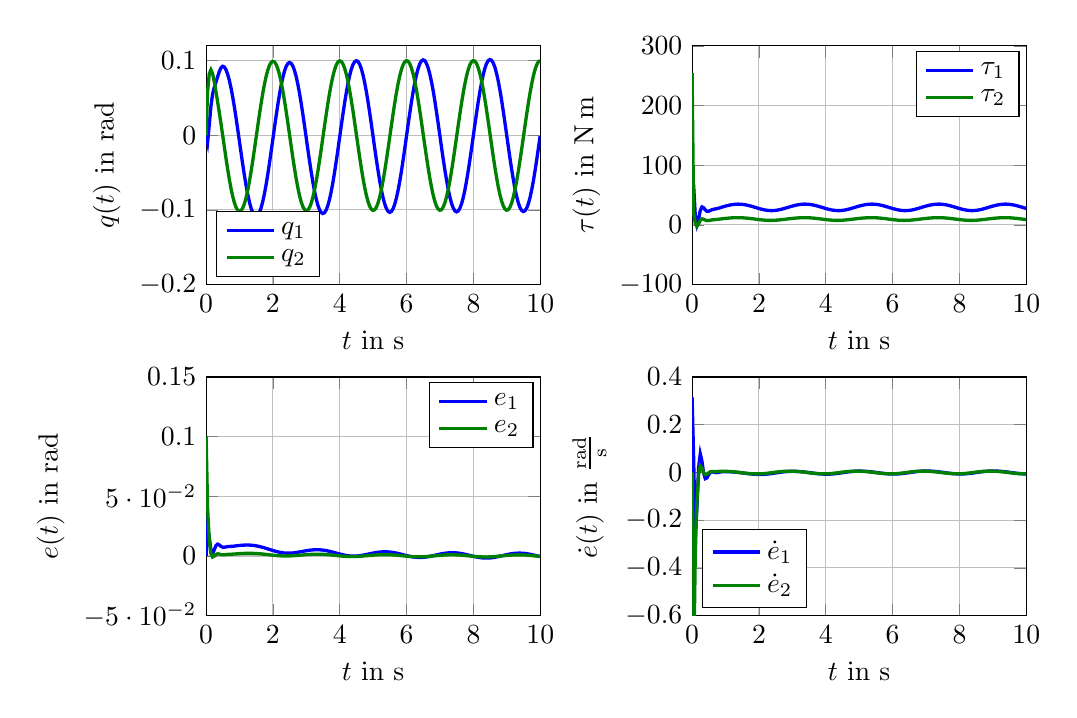
\begin{tikzpicture}

\begin{axis}[%
width=0.35\textwidth,
height=0.25\textwidth,
scale only axis,
xmin=0,
xmax=10,
xlabel={$t$ in $\mathrm{s}$},
xmajorgrids,
ymin=-0.2,
ymax=0.12,
ylabel={$q(t)$ in $\mathrm{rad}$},
ymajorgrids,
name=plot1,
legend style={at={(0.03,0.03)},anchor=south west,draw=black,fill=white,legend cell align=left}
]
\addplot [
color=blue,
solid,
line width=1.2pt
]
table[row sep=crcr]{
0 0\\
0.0446451031238306 -0.00960040788822535\\
0.0946451031238306 0.0134630568048844\\
0.144645103123831 0.0389430341544383\\
0.194645103123831 0.0551996326932098\\
0.244645103123831 0.0642844388846784\\
0.294645103123831 0.0712154598839009\\
0.344645103123831 0.0784178738390533\\
0.394645103123831 0.0853538576440008\\
0.444645103123831 0.0904341589197851\\
0.494645103123831 0.0925948700684472\\
0.544645103123831 0.0916737310624652\\
0.594645103123831 0.0880172658952059\\
0.644645103123831 0.0820150522665913\\
0.694645103123831 0.0739091302546367\\
0.744645103123831 0.0638459188053572\\
0.794645103123831 0.051995208189368\\
0.844645103123831 0.0386151942797427\\
0.894645103123831 0.0240462990298431\\
0.944645103123831 0.00867299301218166\\
0.994645103123831 -0.00710861292159371\\
1.04464510312383 -0.022905216203882\\
1.09464510312382 -0.0383296468408529\\
1.14464510312382 -0.0530034341271928\\
1.19464510312381 -0.066563462907421\\
1.2446451031238 -0.0786718180068744\\
1.2946451031238 -0.0890259025866807\\
1.34464510312379 -0.0973668589514507\\
1.39464510312379 -0.103485915266409\\
1.44464510312378 -0.107229107789859\\
1.49464510312378 -0.108500791460285\\
1.54464510312377 -0.107265989563979\\
1.59464510312377 -0.103551396037449\\
1.64464510312376 -0.0974448445753663\\
1.69464510312375 -0.0890931890518586\\
1.74464510312375 -0.0786986669747199\\
1.79464510312374 -0.0665138847727689\\
1.84464510312374 -0.052835582917441\\
1.89464510312373 -0.0379973435653536\\
1.94464510312373 -0.0223614138241628\\
1.99464510312372 -0.0063098353157315\\
2.04464510312372 0.00976491170367571\\
2.09464510312371 0.0254695293466241\\
2.14464510312371 0.0404195621064004\\
2.1946451031237 0.0542488682516761\\
2.24464510312369 0.0666186760875545\\
2.29464510312369 0.077226002351773\\
2.34464510312368 0.0858112179220165\\
2.39464510312368 0.0921645598818385\\
2.44464510312367 0.0961314102642524\\
2.49464510312367 0.0976161911048758\\
2.54464510312366 0.0965847625034661\\
2.59464510312366 0.0930652539528186\\
2.64464510312365 0.0871473070443494\\
2.69464510312364 0.0789797568493548\\
2.74464510312364 0.068766826512672\\
2.79464510312363 0.056762951813076\\
2.84464510312363 0.0432663873618756\\
2.89464510312362 0.0286117726212276\\
2.94464510312362 0.0131618541779096\\
2.99464510312361 -0.00270142811767688\\
3.04464510312361 -0.0185862777013642\\
3.0946451031236 -0.0341005848082168\\
3.1446451031236 -0.048861461124077\\
3.19464510312359 -0.0625045511324883\\
3.24464510312358 -0.0746929086190925\\
3.29464510312358 -0.0851252319161815\\
3.34464510312357 -0.0935432599374744\\
3.39464510312357 -0.0997381441673173\\
3.44464510312356 -0.103555630696728\\
3.49464510312356 -0.104899911875918\\
3.54464510312355 -0.103736039224017\\
3.59464510312355 -0.100090827097346\\
3.64464510312354 -0.0940522186110847\\
3.69464510312353 -0.0857671291128906\\
3.74464510312353 -0.0754378254918537\\
3.79464510312352 -0.0633169392914645\\
3.84464510312352 -0.0497012460811767\\
3.89464510312351 -0.034924371793097\\
3.94464510312351 -0.0193486086389502\\
3.9946451031235 -0.00335603943230162\\
4.04464510312352 0.0126608192825677\\
4.09464510312353 0.0283086368505673\\
4.14464510312355 0.0432029271183274\\
4.19464510312357 0.056977519412756\\
4.24464510312358 0.0692936151223977\\
4.2946451031236 0.0798482065357431\\
4.34464510312362 0.088381642750837\\
4.39464510312363 0.094684141691477\\
4.44464510312365 0.0986010686935272\\
4.49464510312367 0.100036831405821\\
4.54464510312368 0.0989572777240275\\
4.5946451031237 0.0953905269778831\\
4.64464510312372 0.0894262124389444\\
4.69464510312373 0.0812131624305195\\
4.74464510312375 0.0709555945835832\\
4.79464510312377 0.0589079400123957\\
4.84464510312378 0.0453684491034059\\
4.8946451031238 0.0306717571205031\\
4.94464510312382 0.0151806060832535\\
4.99464510312383 -0.000723069452214886\\
5.04464510312385 -0.0166474792466492\\
5.09464510312387 -0.032200521127494\\
5.14464510312388 -0.0469993158044602\\
5.1946451031239 -0.0606795183076083\\
5.24464510312392 -0.0729041945147053\\
5.29464510312393 -0.0833720563582722\\
5.34464510312395 -0.0918248577716936\\
5.39464510312397 -0.0980537665483667\\
5.44464510312398 -0.101904546215867\\
5.494645103124 -0.103281407503694\\
5.54464510312402 -0.102149421053418\\
5.59464510312403 -0.0985354208797094\\
5.64464510312405 -0.0925273700832558\\
5.69464510312407 -0.0842722041193278\\
5.74464510312408 -0.0739722099096774\\
5.7946451031241 -0.0618800387700029\\
5.84464510312412 -0.0482924856104711\\
5.89464510312413 -0.0335431951182197\\
5.94464510312415 -0.0179944775388961\\
5.99464510312417 -0.00202843288357474\\
6.04464510312418 0.0139624060368584\\
6.0946451031242 0.0295846933054376\\
6.14464510312422 0.0444539285658781\\
6.19464510312423 0.058203928037664\\
6.24464510312425 0.0704958811187182\\
6.29464510312427 0.081026769232335\\
6.34464510312428 0.0895369317346893\\
6.3946451031243 0.0958165779190013\\
6.44464510312432 0.0997110655790752\\
6.49464510312433 0.101124795874209\\
6.54464510312435 0.100023611210112\\
6.59464510312437 0.0964356263520447\\
6.64464510312438 0.0904504708338887\\
6.6946451031244 0.0822169699432275\\
6.74464510312442 0.0719393388275605\\
6.79464510312443 0.0598720064999155\\
6.84464510312445 0.0463132214449939\\
6.89464510312447 0.0315976170385448\\
6.94464510312448 0.0160879332470074\\
6.9946451031245 0.000166102246819853\\
7.04464510312452 -0.0157760885656808\\
7.09464510312453 -0.0313465404305352\\
7.14464510312455 -0.0461623781134704\\
7.19464510312457 -0.0598592613850555\\
7.24464510312458 -0.0721002615585205\\
7.2946451031246 -0.0825840966800556\\
7.34464510312462 -0.0910525274351131\\
7.39464510312463 -0.097296728949082\\
7.44464510312465 -0.101162472588629\\
7.49464510312467 -0.102553977346306\\
7.54464510312468 -0.101436322460882\\
7.5946451031247 -0.0978363507851163\\
7.64464510312472 -0.0918420344047376\\
7.69464510312473 -0.0836003178147424\\
7.74464510312475 -0.0733134969426419\\
7.79464510312477 -0.0612342319924943\\
7.84464510312479 -0.0476593265685255\\
7.8946451031248 -0.0329224337883353\\
7.94464510312482 -0.0173858720036014\\
7.99464510312484 -0.00143174895522807\\
8.04464510312481 0.0145473952346649\\
8.09464510312479 0.0301582077895753\\
8.14464510312476 0.0450161819696799\\
8.19464510312473 0.0587551281032655\\
8.2446451031247 0.0710362301989121\\
8.29464510312467 0.0815564647962579\\
8.34464510312465 0.0900561668725428\\
8.39464510312462 0.096325541841365\\
8.44464510312459 0.100209944106\\
8.49464510312456 0.101613771908167\\
8.54464510312454 0.100502865185196\\
8.59464510312451 0.0969053366499209\\
8.64464510312448 0.0909108141554395\\
8.69464510312445 0.0826681216241372\\
8.74464510312442 0.0723814730866479\\
8.7946451031244 0.0603052966110803\\
8.84464510312437 0.0467378398270275\\
8.89464510312434 0.0320137352613905\\
8.94464510312431 0.0164957219577284\\
8.99464510312429 0.000565731022916256\\
9.04464510312426 -0.0153844514244159\\
9.09464510312423 -0.0309627281580432\\
9.1446451031242 -0.0457862257666327\\
9.19464510312418 -0.05949060615139\\
9.24464510312415 -0.0717389430686002\\
9.29464510312412 -0.0822299573124153\\
9.34464510312409 -0.0907054126032661\\
9.39464510312406 -0.0969564873622503\\
9.44464510312404 -0.100828956479729\\
9.49464510312401 -0.102227042662545\\
9.54464510312398 -0.101115829013968\\
9.59464510312395 -0.0975221623595255\\
9.64464510312393 -0.0915340188237321\\
9.6946451031239 -0.0832983469649026\\
9.74464510312387 -0.0730174467585336\\
9.79464510312384 -0.0609439824038272\\
9.84464510312382 -0.0473747614127432\\
9.89464510312379 -0.0326434406920652\\
9.94464510312376 -0.0171123422367694\\
9.99464510312373 -0.00116357726192095\\
};
\addlegendentry{$q_1$};

\addplot [
color=green!50!black,
solid,
line width=1.2pt
]
table[row sep=crcr]{
0 0\\
0.0446451031238306 0.0583270508805101\\
0.0946451031238306 0.0825061114103156\\
0.144645103123831 0.0878355442979262\\
0.194645103123831 0.0827490903101578\\
0.244645103123831 0.0719438748302113\\
0.294645103123831 0.0588253730799328\\
0.344645103123831 0.04505599702906\\
0.394645103123831 0.0308965937895151\\
0.444645103123831 0.016126666494336\\
0.494645103123831 0.000725323391264751\\
0.544645103123831 -0.0149726698752043\\
0.594645103123831 -0.0304469276418297\\
0.644645103123831 -0.0451930620815934\\
0.694645103123831 -0.0588098555026043\\
0.744645103123831 -0.0709850566573538\\
0.794645103123831 -0.0814522727635832\\
0.844645103123831 -0.0899688687124489\\
0.894645103123831 -0.0963218447054601\\
0.944645103123831 -0.100345370065763\\
0.994645103123831 -0.101934319029234\\
1.04464510312383 -0.101048773077533\\
1.09464510312382 -0.0977123533590824\\
1.14464510312382 -0.0920087440599811\\
1.19464510312381 -0.0840785244841281\\
1.2446451031238 -0.0741160840710849\\
1.2946451031238 -0.062365589554723\\
1.34464510312379 -0.0491153876422478\\
1.39464510312379 -0.034690908177098\\
1.44464510312378 -0.0194464920546748\\
1.49464510312378 -0.00375656418783946\\
1.54464510312377 0.0119935737126574\\
1.59464510312377 0.0274171563865362\\
1.64464510312376 0.0421354089092428\\
1.69464510312375 0.0557868372551368\\
1.74464510312375 0.0680361201734342\\
1.79464510312374 0.0785823655069707\\
1.84464510312374 0.0871665163751151\\
1.89464510312373 0.0935777239174234\\
1.94464510312373 0.0976585343029203\\
1.99464510312372 0.0993087671260999\\
2.04464510312372 0.0984879924652189\\
2.09464510312371 0.0952165465034392\\
2.14464510312371 0.089575060457296\\
2.1946451031237 0.0817025131819875\\
2.24464510312369 0.0717928528202124\\
2.29464510312369 0.0600902664248259\\
2.34464510312368 0.0468832083011546\\
2.39464510312368 0.0324973276906922\\
2.44464510312367 0.0172874640089535\\
2.49464510312367 0.00162890256675647\\
2.54464510312366 -0.0140918952615356\\
2.59464510312366 -0.0294868570643241\\
2.64464510312365 -0.0441759185160395\\
2.69464510312364 -0.0577964513666644\\
2.74464510312364 -0.0700122582591279\\
2.79464510312363 -0.0805219031702195\\
2.84464510312363 -0.089066164533947\\
2.89464510312362 -0.0954344230275548\\
2.94464510312362 -0.0994698263350335\\
2.99464510312361 -0.101073107412957\\
3.04464510312361 -0.100204969261974\\
3.0946451031236 -0.0968869864860277\\
3.1446451031236 -0.0912010108137258\\
3.19464510312359 -0.0832871034132408\\
3.24464510312358 -0.0733400507177815\\
3.29464510312358 -0.0616045522884188\\
3.34464510312357 -0.0483691987924509\\
3.39464510312357 -0.0339593852979191\\
3.44464510312356 -0.0187293295267451\\
3.49464510312356 -0.0030533860769795\\
3.54464510312355 0.0126831346343249\\
3.59464510312355 0.0280934205239734\\
3.64464510312354 0.0427986545150984\\
3.69464510312353 0.0564373204636379\\
3.74464510312353 0.0686740885542461\\
3.79464510312352 0.0792080601956145\\
3.84464510312352 0.0877801683928651\\
3.89464510312351 0.0941795510990929\\
3.94464510312351 0.0982487413079596\\
3.9946451031235 0.0998875476309786\\
4.04464510312352 0.0990555317438133\\
4.09464510312353 0.0957730233762496\\
4.14464510312355 0.0901206485709684\\
4.19464510312357 0.0822373820038985\\
4.24464510312358 0.0723171686419995\\
4.2946451031236 0.0606041934244752\\
4.34464510312362 0.0473869095716257\\
4.39464510312363 0.0329909661438154\\
4.44464510312365 0.0177712031265418\\
4.49464510312367 0.00210290701846644\\
4.54464510312368 -0.0136274591069753\\
4.5946451031237 -0.0290318207259942\\
4.64464510312372 -0.043730111097043\\
4.69464510312373 -0.0573596993798262\\
4.74464510312375 -0.069584385600293\\
4.79464510312377 -0.0801027312493073\\
4.84464510312378 -0.0886555125643298\\
4.8946451031238 -0.0950321084649561\\
4.94464510312382 -0.0990756654485184\\
4.99464510312383 -0.100686915963261\\
5.04464510312385 -0.0998265632572789\\
5.09464510312387 -0.0965161829831684\\
5.14464510312388 -0.0908376287338268\\
5.1946451031239 -0.0829309643443957\\
5.24464510312392 -0.0729909796824348\\
5.29464510312393 -0.0612623784583575\\
5.34464510312395 -0.0480337561387753\\
5.39464510312397 -0.0336305131664437\\
5.44464510312398 -0.0184068731308785\\
5.494645103124 -0.00273719690053082\\
5.54464510312402 0.0129931985321968\\
5.59464510312403 0.0283974943095993\\
5.64464510312405 0.0430968664942548\\
5.69464510312407 0.0567297921140725\\
5.74464510312408 0.0689609346788596\\
5.7946451031241 0.0794893891936367\\
5.84464510312412 0.0880560826406951\\
5.89464510312413 0.0944501474265877\\
5.94464510312415 0.0985141115507106\\
5.99464510312417 0.100147779235314\\
6.04464510312418 0.0993107083995345\\
6.0946451031242 0.0960232256527195\\
6.14464510312422 0.0903659545350253\\
6.19464510312423 0.0824778678026604\\
6.24464510312425 0.0725529090391468\\
6.29464510312427 0.0608352622841464\\
6.34464510312428 0.0476133802887096\\
6.3946451031243 0.0332129120225067\\
6.44464510312432 0.0179886977102029\\
6.49464510312433 0.00231602437317465\\
6.54464510312435 -0.0134186441548615\\
6.59464510312437 -0.0288272324005984\\
6.64464510312438 -0.0435296725368688\\
6.6946451031244 -0.057163332561025\\
6.74464510312442 -0.069392011325406\\
6.79464510312443 -0.0799142692057291\\
6.84464510312445 -0.0884708814534163\\
6.89464510312447 -0.0948512261984972\\
6.94464510312448 -0.0988984494049955\\
6.9946451031245 -0.100513283292678\\
7.04464510312452 -0.0996564312209595\\
7.09464510312453 -0.0963494693140237\\
7.14464510312455 -0.0906742520031494\\
7.19464510312457 -0.0827708443228807\\
7.24464510312458 -0.0728340376853824\\
7.2946451031246 -0.0611085376673451\\
7.34464510312462 -0.0478829418940797\\
7.39464510312463 -0.0334826532258874\\
7.44464510312465 -0.0182618978915011\\
7.49464510312467 -0.00259503957968466\\
7.54464510312468 0.0131326017598263\\
7.5946451031247 0.0285342042226054\\
7.64464510312472 0.0432309407860344\\
7.69464510312473 0.0568612854076959\\
7.74464510312475 0.0690898985962005\\
7.79464510312477 0.0796158724775426\\
7.84464510312479 0.0881801313264288\\
7.8946451031248 0.0945718050561322\\
7.94464510312482 0.0986334194211728\\
7.99464510312484 0.100264776670965\\
8.04464510312481 0.0994254330362503\\
8.09464510312479 0.0961357137238644\\
8.14464510312476 0.0904762411491128\\
8.19464510312473 0.0825859872051965\\
8.2446451031247 0.0726588948535379\\
8.29464510312467 0.0609391477290518\\
8.34464510312465 0.0477151983713094\\
8.39464510312462 0.0333126957085383\\
8.44464510312459 0.0180864800721422\\
8.49464510312456 0.00241183871763908\\
8.54464510312454 -0.013324764180337\\
8.59464510312451 -0.0287352527224689\\
8.64464510312448 -0.0434395585943364\\
8.69464510312445 -0.0570750492714564\\
8.74464510312442 -0.0693055230791642\\
8.7946451031244 -0.07982953989234\\
8.84464510312437 -0.0883878745194966\\
8.89464510312434 -0.094769904735976\\
8.94464510312431 -0.0988187762662332\\
8.99464510312429 -0.100435221227443\\
9.04464510312426 -0.0995799430291502\\
9.09464510312423 -0.0962745180076159\\
9.1446451031242 -0.0906008009710978\\
9.19464510312418 -0.0826988574934405\\
9.24464510312415 -0.0727634796813267\\
9.29464510312412 -0.061039373950607\\
9.34464510312409 -0.0478151388972405\\
9.39464510312406 -0.0334161784685597\\
9.44464510312404 -0.0181967200799888\\
9.49464510312401 -0.00253112868838479\\
9.54464510312398 0.0131952744268493\\
9.59464510312395 0.0285956659914732\\
9.64464510312393 0.0432912175958049\\
9.6946451031239 0.0569204018171021\\
9.74464510312387 0.0691478778147813\\
9.79464510312384 0.0796727364206145\\
9.84464510312382 0.0882359006921986\\
9.89464510312379 0.0946264994220656\\
9.94464510312376 0.0986870573556784\\
9.99464510312373 0.100317375855688\\
};
\addlegendentry{$q_2$};

\end{axis}

\begin{axis}[%
width=0.35\textwidth,
height=0.25\textwidth,
scale only axis,
xmin=0,
xmax=10,
xlabel={$t$ in $\mathrm{s}$},
xmajorgrids,
ymin=-0.05,
ymax=0.15,
ylabel={$e(t)$ in $\mathrm{rad}$},
ymajorgrids,
name=plot3,
at=(plot1.below south west),
anchor=above north west,
legend style={draw=black,fill=white,legend cell align=left}
]
\addplot [
color=blue,
solid,
line width=1.2pt
]
table[row sep=crcr]{
0 0\\
0.0446451031238306 0.0235801405090039\\
0.0946451031238306 0.0158343921424181\\
0.144645103123831 0.00495073069364698\\
0.194645103123831 0.00220963789004475\\
0.244645103123831 0.00522673066154036\\
0.294645103123831 0.00868601293670856\\
0.344645103123831 0.00990646281731856\\
0.394645103123831 0.00921850454798617\\
0.444645103123831 0.00805754338297485\\
0.494645103123831 0.00739097975917249\\
0.544645103123831 0.00734428283324746\\
0.594645103123831 0.00759475994453986\\
0.644645103123831 0.00783670012289185\\
0.694645103123831 0.00796990033988515\\
0.744645103123831 0.00804425652004331\\
0.794645103123831 0.0081359371605868\\
0.844645103123831 0.00827629273242057\\
0.894645103123831 0.00845090561036603\\
0.944645103123831 0.0086297402257927\\
0.994645103123831 0.00879082404053496\\
1.04464510312383 0.00892548358310477\\
1.09464510312382 0.00903219789355343\\
1.14464510312382 0.00910966927911185\\
1.19464510312381 0.00915419232417179\\
1.2446451031238 0.00916064846066164\\
1.2946451031238 0.00912442976607722\\
1.34464510312379 0.00904252229508437\\
1.39464510312379 0.00891355307442682\\
1.44464510312378 0.00873740548710117\\
1.49464510312378 0.00851494163266514\\
1.54464510312377 0.00824797566826342\\
1.59464510312377 0.00793937019769742\\
1.64464510312376 0.00759309218587338\\
1.69464510312375 0.00721415845732304\\
1.74464510312375 0.00680849164930153\\
1.79464510312374 0.00638273942279218\\
1.84464510312374 0.00594409590525191\\
1.89464510312373 0.00550013892511518\\
1.94464510312373 0.00505868058615628\\
1.99464510312372 0.00462762419675582\\
2.04464510312372 0.00421482091706721\\
2.09464510312371 0.00382791960064227\\
2.14464510312371 0.00347420274164937\\
2.1946451031237 0.00316040233154485\\
2.24464510312369 0.00289249345863334\\
2.29464510312369 0.0026754704688097\\
2.34464510312368 0.00251311873433364\\
2.39464510312368 0.00240780231013282\\
2.44464510312367 0.0023602920384989\\
2.49464510312367 0.00236965872274296\\
2.54464510312366 0.00243325139225402\\
2.59464510312366 0.00254677188694327\\
2.64464510312365 0.00270444534515868\\
2.69464510312364 0.00289927374520066\\
2.74464510312364 0.0031233488127704\\
2.79464510312363 0.00336819353692835\\
2.84464510312363 0.0036250996503441\\
2.89464510312362 0.00388543201904356\\
2.94464510312362 0.00414087906013105\\
2.99464510312361 0.00438363923668711\\
3.04464510312361 0.00460654508065556\\
3.0946451031236 0.00480313586098348\\
3.1446451031236 0.00496769627605822\\
3.19464510312359 0.00509528054929569\\
3.24464510312358 0.00518173907292956\\
3.29464510312358 0.00522375909561962\\
3.34464510312357 0.00521892328114046\\
3.39464510312357 0.00516578197535719\\
3.44464510312356 0.00506392839398254\\
3.49464510312356 0.00491406204829968\\
3.54464510312355 0.00471802532829166\\
3.59464510312355 0.00447880125757437\\
3.64464510312354 0.00420046622156145\\
3.69464510312353 0.00388809851831526\\
3.74464510312353 0.00354765016638722\\
3.79464510312352 0.00318579394143249\\
3.84464510312352 0.00280975906892662\\
3.89464510312351 0.00242716715279301\\
3.94464510312351 0.00204587540087547\\
3.9946451031235 0.00167382831325674\\
4.04464510312352 0.00131891333811289\\
4.09464510312353 0.000988812096645572\\
4.14464510312355 0.000690837729678442\\
4.19464510312357 0.000431751170430525\\
4.24464510312358 0.000217554423765018\\
4.2946451031236 5.32662848227172e-05\\
4.34464510312362 -5.73060944967507e-05\\
4.39464510312363 -0.000111779499510273\\
4.44464510312365 -0.000109366390777105\\
4.49464510312367 -5.09815782022138e-05\\
4.54464510312368 6.07361716916666e-05\\
4.5946451031237 0.000221498861874725\\
4.64464510312372 0.000425539950554624\\
4.69464510312373 0.000665868164020117\\
4.74464510312375 0.000934580741835139\\
4.79464510312377 0.00122320533757542\\
4.84464510312378 0.00152303790877074\\
4.8946451031238 0.00182544751971553\\
4.94464510312382 0.00212212715472552\\
4.99464510312383 0.00240528057115552\\
5.04464510312385 0.00266774662586463\\
5.09464510312387 0.00290307218018088\\
5.14464510312388 0.0031055509563601\\
5.1946451031239 0.00327024772433602\\
5.24464510312392 0.00339302496846716\\
5.29464510312393 0.00347058353764343\\
5.34464510312395 0.00350052111530415\\
5.39464510312397 0.00348140435636596\\
5.44464510312398 0.00341284391309833\\
5.494645103124 0.00329555767607322\\
5.54464510312402 0.00313140715771316\\
5.59464510312403 0.00292339503998229\\
5.64464510312405 0.00267561769380288\\
5.69464510312407 0.00239317352484841\\
5.74464510312408 0.00208203458433207\\
5.7946451031241 0.0017488934201158\\
5.84464510312412 0.00140099859838708\\
5.89464510312413 0.00104599047810054\\
5.94464510312415 0.000691744301020487\\
5.99464510312417 0.000346221764739064\\
6.04464510312418 1.7326584029977e-05\\
6.0946451031242 -0.000287244358023991\\
6.14464510312422 -0.000560163717683811\\
6.19464510312423 -0.000794657454305576\\
6.24464510312425 -0.000984711572404692\\
6.29464510312427 -0.00112529641164301\\
6.34464510312428 -0.00121259507825068\\
6.3946451031243 -0.00124421572696637\\
6.44464510312432 -0.00121936327628884\\
6.49464510312433 -0.00113894604658681\\
6.54464510312435 -0.00100559731442171\\
6.59464510312437 -0.000823600512348394\\
6.64464510312438 -0.000598718444481797\\
6.6946451031244 -0.00033793934880845\\
6.74464510312442 -4.91635022879661e-05\\
6.79464510312443 0.000259138849887833\\
6.84464510312445 0.000578265566997492\\
6.89464510312447 0.000899587601475245\\
6.94464510312448 0.00121479999076509\\
6.9946451031245 0.00151610887191105\\
7.04464510312452 0.00179635594468869\\
7.09464510312453 0.00204909148302139\\
7.14464510312455 0.0022686132651819\\
7.19464510312457 0.00244999080161133\\
7.24464510312458 0.00258909201213167\\
7.2946451031246 0.00268262385930053\\
7.34464510312462 0.00272819077862532\\
7.39464510312463 0.00272436675701306\\
7.44464510312465 0.00267077028582483\\
7.49464510312467 0.0025681275186821\\
7.54464510312468 0.00241830856520664\\
7.5946451031247 0.00222432494545073\\
7.64464510312472 0.00199028201537688\\
7.69464510312473 0.00172128722038349\\
7.74464510312475 0.00142332161744242\\
7.79464510312477 0.0011030866427747\\
7.84464510312479 0.000767839556626911\\
7.8946451031248 0.000425229148414384\\
7.94464510312482 8.3138765932543e-05\\
7.99464510312484 -0.000250462163398048\\
8.04464510312481 -0.000567662613581026\\
8.09464510312479 -0.0008607588419864\\
8.14464510312476 -0.00112241712133306\\
8.19464510312473 -0.00134585751977968\\
8.2446451031247 -0.00152506065249673\\
8.29464510312467 -0.00165499197548921\\
8.34464510312465 -0.00173183021605076\\
8.39464510312462 -0.00175317964929769\\
8.44464510312459 -0.00171824180319845\\
8.49464510312456 -0.00162792208054374\\
8.54464510312454 -0.00148485128951474\\
8.59464510312451 -0.00129331081023751\\
8.64464510312448 -0.00105906176604582\\
8.69464510312445 -0.000789091029727296\\
8.74464510312442 -0.000491297761377102\\
8.7946451031244 -0.000174151261267554\\
8.84464510312437 0.000153647184986491\\
8.89464510312434 0.000483469378667181\\
8.94464510312431 0.000807011280096588\\
8.99464510312429 0.00111648009588216\\
9.04464510312426 0.00140471880350436\\
9.09464510312423 0.00166527921062076\\
9.1446451031242 0.00189246091844226\\
9.19464510312418 0.00208133556804671\\
9.24464510312415 0.00222777352230996\\
9.29464510312412 0.00232848449175127\\
9.34464510312409 0.00238107594685567\\
9.39464510312406 0.00238412517023946\\
9.44464510312404 0.00233725417695781\\
9.49464510312401 0.00224119283492448\\
9.54464510312398 0.00209781511826231\\
9.59464510312395 0.00191013651979104\\
9.64464510312393 0.00168226643426204\\
9.6946451031239 0.00141931637039276\\
9.74464510312387 0.00112727143314154\\
9.79464510312384 0.00081283705387529\\
9.84464510312382 0.000483274400575391\\
9.89464510312379 0.000146236051842837\\
9.94464510312376 -0.000190391001227402\\
9.99464510312373 -0.000518633857051535\\
};
\addlegendentry{$e_1$};

\addplot [
color=green!50!black,
solid,
line width=1.2pt
]
table[row sep=crcr]{
0 0.1\\
0.0446451031238306 0.0406909630152025\\
0.0946451031238306 0.0131059144294302\\
0.144645103123831 0.00201620809155695\\
0.194645103123831 -0.000870059715635849\\
0.244645103123831 -5.36995048107392e-05\\
0.294645103123831 0.00130577227002205\\
0.344645103123831 0.00183548998310341\\
0.394645103123831 0.00160061085069423\\
0.444645103123831 0.00117606674363846\\
0.494645103123831 0.000956887727676649\\
0.544645103123831 0.000992937254425671\\
0.594645103123831 0.00114947869452719\\
0.644645103123831 0.00129929723350811\\
0.694645103123831 0.00140058491934962\\
0.744645103123831 0.00147388711113497\\
0.794645103123831 0.00155079994297361\\
0.844645103123831 0.00164453205607694\\
0.894645103123831 0.00174948251347314\\
0.944645103123831 0.00185366776300337\\
0.994645103123831 0.00194846920161385\\
1.04464510312383 0.00203075918181969\\
1.09464510312382 0.00210032751933575\\
1.14464510312382 0.00215699167049585\\
1.19464510312381 0.0021994938896024\\
1.2446451031238 0.00222590874567859\\
1.2946451031238 0.00223444420476004\\
1.34464510312379 0.00222390063007403\\
1.39464510312379 0.00219370353687585\\
1.44464510312378 0.00214375881668528\\
1.49464510312378 0.00207435306888111\\
1.54464510312377 0.00198615890810263\\
1.59464510312377 0.0018802925607468\\
1.64464510312376 0.00175835593882259\\
1.69464510312375 0.00162243332809829\\
1.74464510312375 0.00147504937276617\\
1.79464510312374 0.00131910731362238\\
1.84464510312374 0.00115782028124307\\
1.89464510312373 0.000994638274553553\\
1.94464510312373 0.000833167999834031\\
1.99464510312372 0.000677082701519172\\
2.04464510312372 0.000530021430498795\\
2.09464510312371 0.000395479336317631\\
2.14464510312371 0.000276691932204504\\
2.1946451031237 0.000176517412558017\\
2.24464510312369 9.7322505218031e-05\\
2.29464510312369 4.08789251646474e-05\\
2.34464510312368 8.27871104973343e-06\\
2.39464510312368 -1.23050437374206e-07\\
2.44464510312367 1.52692290701223e-05\\
2.49464510312367 5.33085522365301e-05\\
2.54464510312366 0.000112162640809807\\
2.59464510312366 0.000189408117074165\\
2.64464510312365 0.000282153668005242\\
2.69464510312364 0.000387180783457661\\
2.74464510312364 0.00050108871295243\\
2.79464510312363 0.000620430349647177\\
2.84464510312363 0.000741827877605017\\
2.89464510312362 0.000862060835589096\\
2.94464510312362 0.000978124032285185\\
2.99464510312361 0.00108725758533886\\
3.04464510312361 0.00118695536625177\\
3.0946451031236 0.00127496064626072\\
3.1446451031236 0.00134925842421016\\
3.19464510312359 0.00140807281867544\\
3.24464510312358 0.00144987539232702\\
3.29464510312358 0.00147340693840056\\
3.34464510312357 0.00147771178021599\\
3.39464510312357 0.00146218065763167\\
3.44464510312356 0.00142659628868731\\
3.49464510312356 0.00137117495795185\\
3.54464510312355 0.00129659798636667\\
3.59464510312355 0.00120402842324344\\
3.64464510312354 0.00109511033290473\\
3.69464510312353 0.000971950119540446\\
3.74464510312353 0.000837080991904507\\
3.79464510312352 0.000693412624936968\\
3.84464510312352 0.000544168263460654\\
3.89464510312351 0.000392811092861545\\
3.94464510312351 0.000242960994782757\\
3.9946451031235 9.83021966392966e-05\\
4.04464510312352 -3.75178480868099e-05\\
4.09464510312353 -0.000160997536476373\\
4.14464510312355 -0.000268896181446418\\
4.19464510312357 -0.000358351409328841\\
4.24464510312358 -0.000426993316544763\\
4.2946451031236 -0.00047304807446219\\
4.34464510312362 -0.000495422559402756\\
4.39464510312363 -0.000493761503547241\\
4.44464510312365 -0.000468469888511104\\
4.49464510312367 -0.000420695899473244\\
4.54464510312368 -0.000352273513757204\\
4.5946451031237 -0.000265628221268816\\
4.64464510312372 -0.000163653751009879\\
4.69464510312373 -4.95712034031537e-05\\
4.74464510312375 7.32160540926619e-05\\
4.79464510312377 0.000201258428710022\\
4.84464510312378 0.000331175907965053\\
4.8946451031238 0.000459746272972364\\
4.94464510312382 0.000583963145759189\\
4.99464510312383 0.000701066135640957\\
5.04464510312385 0.000808549361567115\\
5.09464510312387 0.00090415714342594\\
5.14464510312388 0.000985876344350864\\
5.1946451031239 0.00105193374988621\\
5.24464510312392 0.00110080435705304\\
5.29464510312393 0.00113123310842829\\
5.34464510312395 0.00114226912664507\\
5.39464510312397 0.00113330852627467\\
5.44464510312398 0.00110413989295129\\
5.494645103124 0.0010549857816424\\
5.54464510312402 0.000986534088639647\\
5.59464510312403 0.000899954637763847\\
5.64464510312405 0.000796898353892461\\
5.69464510312407 0.000679478469242684\\
5.74464510312408 0.00055023486741626\\
5.7946451031241 0.000412083627023774\\
5.84464510312412 0.000268254015718866\\
5.89464510312413 0.000122214765430145\\
5.94464510312415 -2.24092479332721e-05\\
5.99464510312417 -0.000161929407692538\\
6.04464510312418 -0.000292694503837329\\
6.0946451031242 -0.000411199813007815\\
6.14464510312422 -0.000514202145595416\\
6.19464510312423 -0.000598837208211231\\
6.24464510312425 -0.000662733713837807\\
6.29464510312427 -0.000704116934301162\\
6.34464510312428 -0.000721893276671944\\
6.3946451031243 -0.00071570738243705\\
6.44464510312432 -0.000685964472378817\\
6.49464510312433 -0.000633813254391358\\
6.54464510312435 -0.000561088466078693\\
6.59464510312437 -0.000470216546865267\\
6.64464510312438 -0.000364092311372535\\
6.6946451031244 -0.000245938022376262\\
6.74464510312442 -0.000119158220945159\\
6.79464510312443 1.27963850055646e-05\\
6.84464510312445 0.000146544796953196\\
6.89464510312447 0.000278864006445237\\
6.94464510312448 0.000406747102200025\\
6.9946451031245 0.000527433465054558\\
7.04464510312452 0.000638417325276988\\
7.09464510312453 0.000737443474342778\\
7.14464510312455 0.000822499613765473\\
7.19464510312457 0.000891813728491758\\
7.24464510312458 0.000943862360146347\\
7.2946451031246 0.000977392317583578\\
7.34464510312462 0.00099145488213459\\
7.39464510312463 0.000985448585916836\\
7.44464510312465 0.000959164653780636\\
7.49464510312467 0.000912828461006147\\
7.54464510312468 0.000847130861218064\\
7.5946451031247 0.000763244724958471\\
7.64464510312472 0.000662824062301504\\
7.69464510312473 0.000547985175791167\\
7.74464510312475 0.000421270950226232\\
7.79464510312477 0.000285600343244\\
7.84464510312479 0.000144205330083635\\
7.8946451031248 5.57135953802024e-07\\
7.94464510312482 -0.000141717118359183\\
7.99464510312484 -0.00027892684333998\\
8.04464510312481 -0.000407419140580789\\
8.09464510312479 -0.000523687884206411\\
8.14464510312476 -0.000624488759757416\\
8.19464510312473 -0.000706956610836695\\
8.2446451031247 -0.00076871952832748\\
8.29464510312467 -0.000808002379308427\\
8.34464510312465 -0.000823711359372439\\
8.39464510312462 -0.000815491068563039\\
8.44464510312459 -0.000783746834402813\\
8.49464510312456 -0.000729627598927517\\
8.54464510312454 -0.000654968440660889\\
8.59464510312451 -0.00056219622503691\\
8.64464510312448 -0.000454206253932055\\
8.69464510312445 -0.000334221311957941\\
8.74464510312442 -0.000205646467188778\\
8.7946451031244 -7.19329283764281e-05\\
8.84464510312437 6.35378630454569e-05\\
8.89464510312434 0.000197542543936974\\
8.94464510312431 0.000327073963446931\\
8.99464510312429 0.000449371399820778\\
9.04464510312426 0.000561929133456304\\
9.09464510312423 0.000662492167906883\\
9.1446451031242 0.000749048581665954\\
9.19464510312418 0.000819826898980677\\
9.24464510312415 0.000873304355995239\\
9.29464510312412 0.000908228600724571\\
9.34464510312409 0.000923651885149736\\
9.39464510312406 0.00091897382841985\\
9.44464510312404 0.000893986842077948\\
9.49464510312401 0.000848917569499157\\
9.54464510312398 0.000784458193976149\\
9.59464510312395 0.000701782955866165\\
9.64464510312393 0.000602547252307177\\
9.6946451031239 0.000488868766169707\\
9.74464510312387 0.000363291731446239\\
9.79464510312384 0.000228736399997265\\
9.84464510312382 8.84359641709076e-05\\
9.89464510312379 -5.4137230083115e-05\\
9.94464510312376 -0.000195355052922355\\
9.99464510312373 -0.000331526028068588\\
};
\addlegendentry{$e_2$};

\end{axis}

\begin{axis}[%
width=0.35\textwidth,
height=0.25\textwidth,
scale only axis,
xmin=0,
xmax=10,
xlabel={$t$ in $\mathrm{s}$},
xmajorgrids,
ymin=-0.6,
ymax=0.4,
ylabel={$\dot{e}(t)$ in $\mathrm{\frac{rad}{s}}$},
ymajorgrids,
name=plot2,
at=(plot3.right of south east),
anchor=left of south west,
legend style={at={(0.03,0.03)},anchor=south west,draw=black,fill=white,legend cell align=left}
]
\addplot [
color=blue,
solid,
line width=1.2pt
]
table[row sep=crcr]{
0 0.314159265358979\\
0.0446451031238306 0.0685266796561469\\
0.0946451031238306 -0.259996394665134\\
0.144645103123831 -0.144122368646816\\
0.194645103123831 0.0196361343878349\\
0.244645103123831 0.0776538386866259\\
0.294645103123831 0.0473139661938049\\
0.344645103123831 -0.00169624825633447\\
0.394645103123831 -0.0259877535347461\\
0.444645103123831 -0.0229428888594513\\
0.494645103123831 -0.00944034175110291\\
0.544645103123831 0.000344674282025094\\
0.594645103123831 0.00275154961566129\\
0.644645103123831 0.00105551237940676\\
0.694645103123831 -0.000662022605324164\\
0.744645103123831 -0.00069032794670848\\
0.794645103123831 0.000512534241293827\\
0.844645103123831 0.00184839878258858\\
0.894645103123831 0.00266727728666605\\
0.944645103123831 0.00294224304005752\\
0.994645103123831 0.00293263266963795\\
1.04464510312383 0.0028495501201577\\
1.09464510312382 0.00274454167631993\\
1.14464510312382 0.00256849977167439\\
1.19464510312381 0.00226480246178895\\
1.2446451031238 0.0018154429922769\\
1.2946451031238 0.00123655871280376\\
1.34464510312379 0.000555480159131344\\
1.39464510312379 -0.000204706863923515\\
1.44464510312378 -0.00102708485537253\\
1.49464510312378 -0.00189591299539214\\
1.54464510312377 -0.00279233287384226\\
1.59464510312377 -0.00369371700336349\\
1.64464510312376 -0.00457557179313017\\
1.69464510312375 -0.00541381320516346\\
1.74464510312375 -0.00618614330179043\\
1.79464510312374 -0.00687245535738634\\
1.84464510312374 -0.00745476094393688\\
1.89464510312373 -0.0079170829766787\\
1.94464510312373 -0.00824549875172464\\
1.99464510312372 -0.00842834469371845\\
2.04464510312372 -0.00845656271855233\\
2.09464510312371 -0.00832419100450654\\
2.14464510312371 -0.00802899689006864\\
2.1946451031237 -0.00757319837659964\\
2.24464510312369 -0.006964153457478\\
2.29464510312369 -0.00621485133469954\\
2.34464510312368 -0.00534403747550444\\
2.39464510312368 -0.00437584643199368\\
2.44464510312367 -0.00333889147300079\\
2.49464510312367 -0.00226485267615318\\
2.54464510312366 -0.00118669769477072\\
2.59464510312366 -0.000136743719547722\\
2.64464510312365 0.000855191488437768\\
2.69464510312364 0.00176330832310684\\
2.74464510312364 0.0025668268756105\\
2.79464510312363 0.00325037611072232\\
2.84464510312363 0.00380378516392205\\
2.89464510312362 0.00422139466981591\\
2.94464510312362 0.00450108107912878\\
2.99464510312361 0.00464321916607408\\
3.04464510312361 0.00464979364438711\\
3.0946451031236 0.00452381667225177\\
3.1446451031236 0.00426912821473729\\
3.19464510312359 0.00389056837571167\\
3.24464510312358 0.00339443213928792\\
3.29464510312358 0.00278906144713922\\
3.34464510312357 0.00208540612560135\\
3.39464510312357 0.00129739681722053\\
3.44464510312356 0.000442016365766233\\
3.49464510312356 -0.000460978374013063\\
3.54464510312355 -0.0013896587149733\\
3.59464510312355 -0.00232075931728357\\
3.64464510312354 -0.00323061312520509\\
3.69464510312353 -0.00409604345044309\\
3.74464510312353 -0.00489509581238243\\
3.79464510312352 -0.00560754478795078\\
3.84464510312352 -0.00621517692303319\\
3.89464510312351 -0.00670191226557076\\
3.94464510312351 -0.0070538684664051\\
3.9946451031235 -0.00725948253479408\\
4.04464510312352 -0.00730978398063287\\
4.09464510312353 -0.00719886470663811\\
4.14464510312355 -0.00692452689291184\\
4.19464510312357 -0.00648902445265243\\
4.24464510312358 -0.00589976076809323\\
4.2946451031236 -0.00516977741521266\\
4.34464510312362 -0.00431787338118683\\
4.39464510312363 -0.00336823415305622\\
4.44464510312365 -0.00234952062164076\\
4.49464510312367 -0.00129345775903034\\
4.54464510312368 -0.000233055584828383\\
4.5946451031237 0.000799329632392737\\
4.64464510312372 0.00177384573508435\\
4.69464510312373 0.00266466486404526\\
4.74464510312375 0.00345098615584286\\
4.79464510312377 0.0041174256386376\\
4.84464510312378 0.00465380780936658\\
4.8946451031238 0.00505447681881532\\
4.94464510312382 0.00531732023364179\\
4.99464510312383 0.00544273061114564\\
5.04464510312385 0.00543271588296734\\
5.09464510312387 0.00529031544328584\\
5.14464510312388 0.00501939903625348\\
5.1946451031239 0.00462483766424221\\
5.24464510312392 0.00411295703515377\\
5.29464510312393 0.00349212852033895\\
5.34464510312395 0.00277332915606196\\
5.39464510312397 0.00197051384448931\\
5.44464510312398 0.00110068619398703\\
5.494645103124 0.000183619954924251\\
5.54464510312402 -0.000758743380335311\\
5.59464510312403 -0.00170312984553844\\
5.64464510312405 -0.00262586791236658\\
5.69464510312407 -0.00350378045404984\\
5.74464510312408 -0.00431491638775675\\
5.7946451031241 -0.00503905726242404\\
5.84464510312412 -0.00565799985539012\\
5.89464510312413 -0.00615567734770511\\
5.94464510312415 -0.00651822303416061\\
5.99464510312417 -0.00673409166692557\\
6.04464510312418 -0.00679433217992803\\
6.0946451031242 -0.0066930571754541\\
6.14464510312422 -0.00642809043320208\\
6.19464510312423 -0.00600170803566058\\
6.24464510312425 -0.00542133582574997\\
6.29464510312427 -0.00470003790042678\\
6.34464510312428 -0.00385663562636737\\
6.3946451031243 -0.00291533652759313\\
6.44464510312432 -0.00190482295500306\\
6.49464510312433 -0.000856840465244244\\
6.54464510312435 0.000195581594352026\\
6.59464510312437 0.00122006934612466\\
6.64464510312438 0.00218675525787443\\
6.6946451031244 0.00306979885093114\\
6.74464510312442 0.00384838986007507\\
6.79464510312443 0.00450713846874384\\
6.84464510312445 0.00503586704986669\\
6.89464510312447 0.00542892130941436\\
6.94464510312448 0.00568419380097684\\
6.9946451031245 0.00580208507347918\\
7.04464510312452 0.00578461349433762\\
7.09464510312453 0.00563483069924381\\
7.14464510312455 0.00535661981806518\\
7.19464510312457 0.00495486574469028\\
7.24464510312458 0.00443590800271582\\
7.2946451031246 0.00380813119912155\\
7.34464510312462 0.00308252460828781\\
7.39464510312463 0.00227305404349513\\
7.44464510312465 0.00139673245173123\\
7.49464510312467 0.000473341181014258\\
7.54464510312468 -0.000475172519319271\\
7.5946451031247 -0.00142553080654791\\
7.64464510312472 -0.00235406014504053\\
7.69464510312473 -0.00323758321578488\\
7.74464510312475 -0.00405415046935537\\
7.79464510312477 -0.00478354659541075\\
7.84464510312479 -0.00540757297718719\\
7.8946451031248 -0.00591016870541328\\
7.94464510312482 -0.00627747411215768\\
7.99464510312484 -0.00649795192895619\\
8.04464510312481 -0.00656265982305354\\
8.09464510312479 -0.00646571970186482\\
8.14464510312476 -0.00620496505323043\\
8.19464510312473 -0.0057826819223597\\
8.2446451031247 -0.00520630624478163\\
8.29464510312467 -0.00448891223649778\\
8.34464510312465 -0.0036493313194326\\
8.39464510312462 -0.00271178091908487\\
8.44464510312459 -0.00170495302907533\\
8.49464510312456 -0.000660602456079999\\
8.54464510312454 0.000388232766420964\\
8.59464510312451 0.00140917084600779\\
8.64464510312448 0.00237233733898293\\
8.69464510312445 0.00325188609266167\\
8.74464510312442 0.00402700261341113\\
8.7946451031244 0.00468229445470819\\
8.84464510312437 0.0052075830318315\\
8.89464510312434 0.00559721474703262\\
8.94464510312431 0.0058490843931342\\
8.99464510312429 0.00596359610945008\\
9.04464510312426 0.00594277295307577\\
9.09464510312423 0.00578967206172148\\
9.1446451031242 0.00550818258220159\\
9.19464510312418 0.00510319565321338\\
9.24464510312415 0.00458105700943434\\
9.29464510312412 0.00395015720838179\\
9.34464510312409 0.00322149102661029\\
9.39464510312406 0.00240902918296357\\
9.44464510312404 0.00152978882287782\\
9.49464510312401 0.000603554709892209\\
9.54464510312398 -0.00034772331894542\\
9.59464510312395 -0.00130076567890511\\
9.64464510312393 -0.00223189793293557\\
9.6946451031239 -0.00311794267677931\\
9.74464510312387 -0.0039369510516504\\
9.79464510312384 -0.00466870916039658\\
9.84464510312382 -0.00529502045798486\\
9.89464510312379 -0.00579982669272905\\
9.94464510312376 -0.00616927136085244\\
9.99464510312373 -0.00639182078114897\\
};
\addlegendentry{$\dot{e}_1$};

\addplot [
color=green!50!black,
solid,
line width=1.2pt
]
table[row sep=crcr]{
0 -0\\
0.0446451031238306 -0.847923818655687\\
0.0946451031238306 -0.346510972201309\\
0.144645103123831 -0.125324824419285\\
0.194645103123831 -0.0100495445816132\\
0.244645103123831 0.02729378788142\\
0.294645103123831 0.0187125329960539\\
0.344645103123831 -0.000143890239945543\\
0.394645103123831 -0.0094533705115592\\
0.444645103123831 -0.00763915231692014\\
0.494645103123831 -0.00157352736798672\\
0.544645103123831 0.00289388635251681\\
0.594645103123831 0.00424842498850769\\
0.644645103123831 0.00384382415937612\\
0.694645103123831 0.00336593498156701\\
0.744645103123831 0.00351912727263945\\
0.794645103123831 0.004111340189691\\
0.844645103123831 0.00468707397026732\\
0.894645103123831 0.00497738139380544\\
0.944645103123831 0.00497202486938326\\
0.994645103123831 0.00478025090545529\\
1.04464510312383 0.00449257805601473\\
1.09464510312382 0.00413481013267381\\
1.14464510312382 0.00369242073792381\\
1.19464510312381 0.00314910577625716\\
1.2446451031238 0.00250585846448798\\
1.2946451031238 0.0017790219917444\\
1.34464510312379 0.000990596910815822\\
1.39464510312379 0.000161590784762744\\
1.44464510312378 -0.000689066719598008\\
1.49464510312378 -0.00154274880660538\\
1.54464510312377 -0.00237963525144258\\
1.59464510312377 -0.00317871044361168\\
1.64464510312376 -0.00391880988096843\\
1.69464510312375 -0.00457982437499088\\
1.74464510312375 -0.00514355062839578\\
1.79464510312374 -0.00559416776166807\\
1.84464510312374 -0.00591854082682397\\
1.89464510312373 -0.00610651610865835\\
1.94464510312373 -0.00615125104503483\\
1.99464510312372 -0.00604954102224206\\
2.04464510312372 -0.00580209054071916\\
2.09464510312371 -0.00541369278553452\\
2.14464510312371 -0.00489329443208078\\
2.1946451031237 -0.00425392159990978\\
2.24464510312369 -0.00351243733447543\\
2.29464510312369 -0.00268910302814845\\
2.34464510312368 -0.00180693117675873\\
2.39464510312368 -0.00089084260001443\\
2.44464510312367 3.33284549453028e-05\\
2.49464510312367 0.00093990991358911\\
2.54464510312366 0.00180445709671612\\
2.59464510312366 0.0026047098450071\\
2.64464510312365 0.00332135298604636\\
2.69464510312364 0.00393851648151256\\
2.74464510312364 0.00444398867298526\\
2.79464510312363 0.00482915855153343\\
2.84464510312363 0.00508874236659695\\
2.89464510312362 0.0052203780089153\\
2.94464510312362 0.00522418184939451\\
2.99464510312361 0.00510235545019532\\
3.04464510312361 0.00485890632125525\\
3.0946451031236 0.00449951345920035\\
3.1446451031236 0.00403153216221991\\
3.19464510312359 0.00346410077488718\\
3.24464510312358 0.00280829018513593\\
3.29464510312358 0.00207722822629325\\
3.34464510312357 0.00128613607904887\\
3.39464510312357 0.000452230271533682\\
3.44464510312356 -0.000405532066600989\\
3.49464510312356 -0.00126686059675146\\
3.54464510312355 -0.00211066422659367\\
3.59464510312355 -0.00291566496874335\\
3.64464510312354 -0.00366104347917906\\
3.69464510312353 -0.00432707065998661\\
3.74464510312353 -0.00489569171171947\\
3.79464510312352 -0.00535104484114513\\
3.84464510312352 -0.0056799117563065\\
3.89464510312351 -0.0058721070602908\\
3.94464510312351 -0.00592081634087016\\
3.9946451031235 -0.00582288797583658\\
4.04464510312352 -0.00557907326789514\\
4.09464510312353 -0.00519419666901194\\
4.14464510312355 -0.00467722623627276\\
4.19464510312357 -0.00404120751368581\\
4.24464510312358 -0.003303024382625\\
4.2946451031236 -0.00248295952315414\\
4.34464510312362 -0.00160404496421129\\
4.39464510312363 -0.000691218063067101\\
4.44464510312365 0.00022967334556534\\
4.49464510312367 0.00113294596291769\\
4.54464510312368 0.00199414585664143\\
4.5946451031237 0.00279100563748791\\
4.64464510312372 0.00350420528259121\\
4.69464510312373 0.00411787269434577\\
4.74464510312375 0.00461979723983497\\
4.79464510312377 0.00500137212857865\\
4.84464510312378 0.00525732093713069\\
4.8946451031238 0.00538529172654967\\
4.94464510312382 0.00538541345379317\\
4.99464510312383 0.00525990212743551\\
5.04464510312385 0.00501278093427304\\
5.09464510312387 0.00464974513802374\\
5.14464510312388 0.00417816630346726\\
5.1946451031239 0.00360719854125602\\
5.24464510312392 0.00294792761179061\\
5.29464510312393 0.00221349503396107\\
5.34464510312395 0.00141913427038459\\
5.39464510312397 0.000582072557202606\\
5.44464510312398 -0.000278723993704377\\
5.494645103124 -0.00114295793969182\\
5.54464510312402 -0.00198953312118499\\
5.59464510312403 -0.00279716867648255\\
5.64464510312405 -0.00354504471278883\\
5.69464510312407 -0.00421343398940277\\
5.74464510312408 -0.00478428596834904\\
5.7946451031241 -0.00524174541426684\\
5.84464510312412 -0.00557260266331552\\
5.89464510312413 -0.00576668267664306\\
5.94464510312415 -0.00581718269675822\\
5.99464510312417 -0.00572096356270771\\
6.04464510312418 -0.00547878934334466\\
6.0946451031242 -0.00509549709566348\\
6.14464510312422 -0.00458006693154603\\
6.19464510312423 -0.00394555561434393\\
6.24464510312425 -0.0032088572381771\\
6.29464510312427 -0.0023902636226833\\
6.34464510312428 -0.00151281487579918\\
6.3946451031243 -0.000601455428819508\\
6.44464510312432 0.000317960754679214\\
6.49464510312433 0.00121974516157614\\
6.54464510312435 0.00207943957912521\\
6.59464510312437 0.00287477334538205\\
6.64464510312438 0.00358642428741818\\
6.6946451031244 0.00419851940935867\\
6.74464510312442 0.00469884854090616\\
6.79464510312443 0.00507880677088937\\
6.84464510312445 0.00533312094997199\\
6.89464510312447 0.0054594436985088\\
6.94464510312448 0.00545790962667352\\
6.9946451031245 0.00533074123717469\\
7.04464510312452 0.00508196876574404\\
7.09464510312453 0.00471729479102942\\
7.14464510312455 0.00424409819342253\\
7.19464510312457 0.00367154017529814\\
7.24464510312458 0.00301071318783866\\
7.2946451031246 0.00227476490717954\\
7.34464510312462 0.00147893432140028\\
7.39464510312463 0.000640453483196968\\
7.44464510312465 -0.000221707456462605\\
7.49464510312467 -0.00108724786188336\\
7.54464510312468 -0.001935069297686\\
7.5946451031247 -0.00274388961357092\\
7.64464510312472 -0.00349288867465913\\
7.69464510312473 -0.00416234008037769\\
7.74464510312475 -0.00473419521388896\\
7.79464510312477 -0.00519260179296543\\
7.84464510312479 -0.00552435403683643\\
7.8946451031248 -0.00571928156632055\\
7.94464510312482 -0.00577058686522233\\
7.99464510312484 -0.00567513637507106\\
8.04464510312481 -0.00543369990298152\\
8.09464510312479 -0.00505112017053407\\
8.14464510312476 -0.00453638270604337\\
8.19464510312473 -0.00390254931312209\\
8.2446451031247 -0.00316651867335649\\
8.29464510312467 -0.00234858671151811\\
8.34464510312465 -0.00147179716428358\\
8.39464510312462 -0.000561097640532304\\
8.44464510312459 0.000357655142674107\\
8.49464510312456 0.00125877032897803\\
8.54464510312454 0.00211778778137889\\
8.59464510312451 0.00291243536587854\\
8.64464510312448 0.00362338994149702\\
8.69464510312445 0.00423477810655992\\
8.74464510312442 0.00473438989648062\\
8.7946451031244 0.00511362124261538\\
8.84464510312437 0.00536720046532302\\
8.89464510312434 0.0054927822327371\\
8.94464510312431 0.00549050369500361\\
8.99464510312429 0.00536259027334015\\
9.04464510312426 0.00511307537188204\\
9.09464510312423 0.00474766485771601\\
9.1446451031242 0.00427374090032051\\
9.19464510312418 0.00370046789074271\\
9.24464510312415 0.00303894128868981\\
9.29464510312412 0.00230231153894722\\
9.34464510312409 0.00150582011407069\\
9.39464510312406 0.000666701232304667\\
9.44464510312404 -0.000196073139634823\\
9.49464510312401 -0.00106220093093901\\
9.54464510312398 -0.00191058268376881\\
9.59464510312395 -0.00271993566940443\\
9.64464510312393 -0.0034694396451635\\
9.6946451031239 -0.00413936858924607\\
9.74464510312387 -0.00471167474952125\\
9.79464510312384 -0.00517050717227382\\
9.84464510312382 -0.00550266182307227\\
9.89464510312379 -0.00569797041792433\\
9.94464510312376 -0.00574963779697534\\
9.99464510312373 -0.0056545329201624\\
};
\addlegendentry{$\dot{e}_2$};

\end{axis}

\begin{axis}[%
width=0.35\textwidth,
height=0.25\textwidth,
scale only axis,
xmin=0,
xmax=10,
xlabel={$t$ in $\mathrm{s}$},
xmajorgrids,
ymin=-100,
ymax=300,
ylabel={$\tau(t)$ in $\mathrm{N\,m}$},
ymajorgrids,
at=(plot2.above north west),
anchor=below south west,
legend style={draw=black,fill=white,legend cell align=left}
]
\addplot [
color=blue,
solid,
line width=1.2pt
]
table[row sep=crcr]{
0 31.5415902420415\\
0.0446451031238306 67.5044030294122\\
0.0946451031238306 15.9441978105722\\
0.144645103123831 0.471427870852263\\
0.194645103123831 10.1353910319827\\
0.244645103123831 23.8340242208198\\
0.294645103123831 29.9600163138569\\
0.344645103123831 28.6396891293538\\
0.394645103123831 24.9552038888824\\
0.444645103123831 22.7548524240443\\
0.494645103123831 22.8050601066761\\
0.544645103123831 24.0320568416554\\
0.594645103123831 25.2724278064619\\
0.644645103123831 26.0852682911771\\
0.694645103123831 26.6224758314159\\
0.744645103123831 27.178594842915\\
0.794645103123831 27.9009124624951\\
0.844645103123831 28.7615616080771\\
0.894645103123831 29.6618567388083\\
0.944645103123831 30.5248400661824\\
0.994645103123831 31.3214735616768\\
1.04464510312383 32.0509317866132\\
1.09464510312382 32.7143182886235\\
1.14464510312382 33.3031222662615\\
1.19464510312381 33.8017848112224\\
1.2446451031238 34.1947247947402\\
1.2946451031238 34.4707303020908\\
1.34464510312379 34.6234415008882\\
1.39464510312379 34.6499852758828\\
1.44464510312378 34.5498627178041\\
1.49464510312378 34.3247886012891\\
1.54464510312377 33.9790951560842\\
1.59464510312377 33.5200895943434\\
1.64464510312376 32.9580612041076\\
1.69464510312375 32.3059751277045\\
1.74464510312375 31.5790281029392\\
1.79464510312374 30.7942041173149\\
1.84464510312374 29.9698783113846\\
1.89464510312373 29.1254590894305\\
1.94464510312373 28.2810439680472\\
1.99464510312372 27.4570701414517\\
2.04464510312372 26.673944421891\\
2.09464510312371 25.9516348445624\\
2.14464510312371 25.3092049398757\\
2.1946451031237 24.7642787436616\\
2.24464510312369 24.3324413963907\\
2.29464510312369 24.0266025478917\\
2.34464510312368 23.8563713915473\\
2.39464510312368 23.8275072149799\\
2.44464510312367 23.9415139003001\\
2.49464510312367 24.1954389994026\\
2.54464510312366 24.5819182703377\\
2.59464510312366 25.0894776642921\\
2.64464510312365 25.7030716134962\\
2.69464510312364 26.4048053391244\\
2.74464510312364 27.174765999607\\
2.79464510312363 27.9918774805773\\
2.84464510312363 28.8346983372949\\
2.89464510312362 29.6821004275511\\
2.94464510312362 30.5137928830012\\
2.99464510312361 31.3106863568675\\
3.04464510312361 32.055119853951\\
3.0946451031236 32.7309919272182\\
3.1446451031236 33.3238466648057\\
3.19464510312359 33.8209620886363\\
3.24464510312358 34.2114759268526\\
3.29464510312358 34.4865644938056\\
3.34464510312357 34.6396689219864\\
3.39464510312357 34.6667437894527\\
3.44464510312356 34.56649024613\\
3.49464510312356 34.3405316874659\\
3.54464510312355 33.993495547131\\
3.59464510312355 33.5329784126193\\
3.64464510312354 32.9693900366559\\
3.69464510312353 32.3156904132917\\
3.74464510312353 31.5870483837238\\
3.79464510312352 30.8004568672369\\
3.84464510312352 29.9743374530011\\
3.89464510312351 29.1281567680236\\
3.94464510312351 28.2820617989129\\
3.9946451031235 27.4565253952826\\
4.04464510312352 26.6719808077691\\
4.09464510312353 25.9484186879237\\
4.14464510312355 25.3049232724328\\
4.19464510312357 24.7591363555067\\
4.24464510312358 24.3266561389573\\
4.2946451031236 24.0203996512843\\
4.34464510312362 23.84997772464\\
4.39464510312363 23.8211459133789\\
4.44464510312365 23.9353993396715\\
4.49464510312367 24.1897719775202\\
4.54464510312368 24.5768813811143\\
4.5946451031237 25.0852310022169\\
4.64464510312372 25.6997490230191\\
4.69464510312373 26.402511414311\\
4.74464510312375 27.1735739872563\\
4.79464510312377 27.9918281806717\\
4.84464510312378 28.8358000399056\\
4.8946451031238 29.6843298729084\\
4.94464510312382 30.5170971791762\\
4.99464510312383 31.3149857410415\\
5.04464510312385 32.0603111452463\\
5.09464510312387 32.7369524965721\\
5.14464510312388 33.3304387411514\\
5.1946451031239 33.8280372278493\\
5.24464510312392 34.2188794860538\\
5.29464510312393 34.4941399745996\\
5.34464510312395 34.6472620689229\\
5.39464510312397 34.6742063526906\\
5.44464510312398 34.5736833387705\\
5.494645103124 34.347328687848\\
5.54464510312402 33.999784514155\\
5.59464510312403 33.5386639977937\\
5.64464510312405 32.9743948900016\\
5.69464510312407 32.3199560916267\\
5.74464510312408 31.5905357794375\\
5.7946451031241 30.8031461837493\\
5.84464510312412 29.9762277600193\\
5.89464510312413 29.129265175585\\
5.94464510312415 28.2824222939226\\
5.99464510312417 27.4561873875164\\
6.04464510312418 26.671007433526\\
6.0946451031242 25.9468849184594\\
6.14464510312422 25.3029138706318\\
6.19464510312423 24.7567437190155\\
6.24464510312425 24.3239780617596\\
6.29464510312427 24.0175370304782\\
6.34464510312428 23.8470322365391\\
6.3946451031243 23.8182176844591\\
6.44464510312432 23.9325846438531\\
6.49464510312433 24.1871610012667\\
6.54464510312435 24.5745561099233\\
6.59464510312437 25.0832632934392\\
6.64464510312438 25.6981989372194\\
6.6946451031244 26.4014258776883\\
6.74464510312442 27.1729858492985\\
6.79464510312443 27.9917557142605\\
6.84464510312445 28.8362469074873\\
6.89464510312447 29.685285555297\\
6.94464510312448 30.5185378369885\\
6.9946451031245 31.3168754560268\\
7.04464510312452 32.0626034723318\\
7.09464510312453 32.7395922481551\\
7.14464510312455 33.3333639227447\\
7.19464510312457 33.8311810472777\\
7.24464510312458 34.2221723654452\\
7.2946451031246 34.4975115036347\\
7.34464510312462 34.650642848073\\
7.39464510312463 34.6775296853684\\
7.44464510312465 34.5768867410924\\
7.49464510312467 34.3503551936116\\
7.54464510312468 34.0025837606642\\
7.5946451031247 33.5411930851887\\
7.64464510312472 32.9766190128213\\
7.69464510312473 32.3218489464724\\
7.74464510312475 31.5920797569403\\
7.79464510312477 30.8043323566883\\
7.84464510312479 29.9770556825619\\
7.8946451031248 29.129742511232\\
7.94464510312482 28.2825642918934\\
7.99464510312484 27.456016228701\\
8.04464510312481 26.6705514677133\\
8.09464510312479 25.9461778140598\\
8.14464510312476 25.3019936963227\\
8.19464510312473 24.7556519745483\\
8.2446451031247 24.3227586722531\\
8.29464510312467 24.016235316148\\
8.34464510312465 23.8456938686641\\
8.39464510312462 23.8168876389947\\
8.44464510312459 23.9313061668161\\
8.49464510312456 24.1859746044837\\
8.54464510312454 24.573498621214\\
8.59464510312451 25.082366990407\\
8.64464510312448 25.697490797114\\
8.69464510312445 26.4009269759629\\
8.74464510312442 27.172710935728\\
8.7946451031244 27.9917129878983\\
8.84464510312437 28.8364380010911\\
8.89464510312434 29.6857057277415\\
8.94464510312431 30.519176360185\\
8.99464510312429 31.3177161726901\\
9.04464510312426 32.0636254934804\\
9.09464510312423 32.7407707551012\\
9.1446451031242 33.334671037181\\
9.19464510312418 33.8325867345005\\
9.24464510312415 34.2236453388579\\
9.29464510312412 34.4990201028839\\
9.34464510312409 34.6521558677213\\
9.39464510312406 34.6790171356437\\
9.44464510312404 34.5783205266084\\
9.49464510312401 34.3517096999938\\
9.54464510312398 34.0038363426106\\
9.59464510312395 33.5423244526655\\
9.64464510312393 32.9776135148269\\
9.6946451031239 32.3226947541225\\
9.74464510312387 31.5927689495686\\
9.79464510312384 30.8048609163165\\
9.84464510312382 29.9774234034672\\
9.89464510312379 29.1299528325575\\
9.94464510312376 28.2826240621554\\
9.99464510312373 27.4559354117282\\
};
\addlegendentry{$\tau_1$};

\addplot [
color=green!50!black,
solid,
line width=1.2pt
]
table[row sep=crcr]{
0 254\\
0.0446451031238306 21.5143570301964\\
0.0946451031238306 3.02287545112162\\
0.144645103123831 -2.62307059589928\\
0.194645103123831 1.59993353977356\\
0.244645103123831 7.3617414810419\\
0.294645103123831 9.95089531621318\\
0.344645103123831 9.4457225891546\\
0.394645103123831 7.95885439111903\\
0.444645103123831 7.08584809693414\\
0.494645103123831 7.1430895285643\\
0.544645103123831 7.68383342921317\\
0.594645103123831 8.22463963837131\\
0.644645103123831 8.58198495679319\\
0.694645103123831 8.81828004399951\\
0.744645103123831 9.05536944247716\\
0.794645103123831 9.35455156944567\\
0.844645103123831 9.70501790396228\\
0.894645103123831 10.0669169034112\\
0.944645103123831 10.4095036686852\\
0.994645103123831 10.721863592867\\
1.04464510312383 11.0046794008882\\
1.09464510312382 11.2592944936451\\
1.14464510312382 11.4828912402117\\
1.19464510312381 11.6695324439625\\
1.2446451031238 11.8130746698741\\
1.2946451031238 11.9090092603711\\
1.34464510312379 11.9546936090782\\
1.39464510312379 11.9488200595317\\
1.44464510312378 11.8909913552313\\
1.49464510312378 11.7816931818526\\
1.54464510312377 11.6225045118127\\
1.59464510312377 11.4162933779085\\
1.64464510312376 11.1672707206571\\
1.69464510312375 10.8809134720756\\
1.74464510312375 10.5638222901161\\
1.79464510312374 10.2235620255118\\
1.84464510312374 9.86849602204522\\
1.89464510312373 9.50760359656853\\
1.94464510312373 9.15026848077931\\
1.99464510312372 8.80603391517648\\
2.04464510312372 8.48432745558839\\
2.09464510312371 8.19416246376297\\
2.14464510312371 7.94382565484264\\
2.1946451031237 7.74056332484235\\
2.24464510312369 7.59028334705402\\
2.29464510312369 7.49729426632485\\
2.34464510312368 7.46410488725997\\
2.39464510312368 7.4913062522354\\
2.44464510312367 7.57755239018119\\
2.49464510312367 7.71964714648052\\
2.54464510312366 7.91273298367828\\
2.59464510312366 8.15056564869871\\
2.64464510312365 8.42584813227698\\
2.69464510312364 8.73059043218991\\
2.74464510312364 9.0564597671435\\
2.79464510312363 9.39508961044797\\
2.84464510312363 9.73832460263776\\
2.89464510312362 10.0783903881827\\
2.94464510312362 10.4079903686125\\
2.99464510312361 10.7203428275334\\
3.04464510312361 11.0091798546203\\
3.0946451031236 11.2687328009213\\
3.1446451031236 11.4937274564634\\
3.19464510312359 11.6794064961316\\
3.24464510312358 11.8215884129001\\
3.29464510312358 11.916762914296\\
3.34464510312357 11.9622143569186\\
3.39464510312357 11.9561586733525\\
3.44464510312356 11.8978762874928\\
3.49464510312356 11.7878239122197\\
3.54464510312355 11.6277113833278\\
3.59464510312355 11.4205347627272\\
3.64464510312354 11.1705625115714\\
3.69464510312353 10.8832763019926\\
3.74464510312353 10.5652710748493\\
3.79464510312352 10.2241199046115\\
3.84464510312352 9.86820837136499\\
3.89464510312351 9.50654123840487\\
3.94464510312351 9.14852232024849\\
3.9946451031235 8.80370748657366\\
4.04464510312352 8.48153147286608\\
4.09464510312353 8.19101179737745\\
4.14464510312355 7.94043736286361\\
4.19464510312357 7.73705455665327\\
4.24464510312358 7.5867688368592\\
4.2946451031236 7.49388372242272\\
4.34464510312362 7.46090063509228\\
4.39464510312363 7.48840127026746\\
4.44464510312365 7.57502868791828\\
4.49464510312367 7.71757438794288\\
4.54464510312368 7.91116731419691\\
4.5946451031237 8.1495487530233\\
4.64464510312372 8.42540658815609\\
4.69464510312373 8.73073542214357\\
4.74464510312375 9.05718718952757\\
4.79464510312377 9.39638060466588\\
4.84464510312378 9.74014647856077\\
4.8946451031238 10.0806979269621\\
4.94464510312382 10.4107274414222\\
4.99464510312383 10.7234442625422\\
5.04464510312385 11.0125734734252\\
5.09464510312387 11.2723415451452\\
5.14464510312388 11.4974715322469\\
5.1946451031239 11.6832054760756\\
5.24464510312392 11.8253632482156\\
5.29464510312393 11.9204378215555\\
5.34464510312395 11.9657185520683\\
5.39464510312397 11.9594279298851\\
5.44464510312398 11.9008542965155\\
5.494645103124 11.7904634208473\\
5.54464510312402 11.6299750863348\\
5.59464510312403 11.4223959224439\\
5.64464510312405 11.1720052843167\\
5.69464510312407 10.8842957566096\\
5.74464510312408 10.5658729003141\\
5.7946451031241 10.2243198181269\\
5.84464510312412 9.86803125426875\\
5.89464510312413 9.50602004230664\\
5.94464510312415 9.14769679785141\\
5.99464510312417 8.80262280875066\\
6.04464510312418 8.48023679460866\\
6.0946451031242 8.18955883019985\\
6.14464510312422 7.93887900100092\\
6.19464510312423 7.73544359099862\\
6.24464510312425 7.58515677623784\\
6.29464510312427 7.49231972909217\\
6.34464510312428 7.45943057228356\\
6.3946451031243 7.48706685533858\\
6.44464510312432 7.57386674549359\\
6.49464510312433 7.71661620227975\\
6.54464510312435 7.91043808726972\\
6.59464510312437 8.14906718207719\\
6.64464510312438 8.42518458161025\\
6.6946451031244 8.73077797390847\\
6.74464510312442 9.05749242836251\\
6.79464510312443 9.39694002739487\\
6.84464510312445 9.74094536522603\\
6.89464510312447 10.0817159242372\\
6.94464510312448 10.4119392900371\\
6.9946451031245 10.724820636761\\
7.04464510312452 11.0140818967884\\
7.09464510312453 11.2739473467746\\
7.14464510312455 11.4991388113174\\
7.19464510312457 11.6848980473247\\
7.24464510312458 11.8270455471837\\
7.2946451031246 11.9220757534539\\
7.34464510312462 11.9672802718523\\
7.39464510312463 11.9608845431082\\
7.44464510312465 11.9021804708938\\
7.49464510312467 11.7916378979677\\
7.54464510312468 11.6309810822272\\
7.5946451031247 11.4232214058187\\
7.64464510312472 11.1726431227387\\
7.69464510312473 10.8847437241876\\
7.74464510312475 10.5661335455922\\
7.79464510312477 10.2244001973794\\
7.84464510312479 9.86794254253377\\
7.8946451031248 9.50577704126285\\
7.94464510312482 9.14731736505474\\
7.99464510312484 8.80212723590606\\
8.04464510312481 8.47964716302135\\
8.09464510312479 8.18889836929026\\
8.14464510312476 7.93817147108249\\
8.19464510312473 7.73471270558384\\
8.2446451031247 7.58442567262293\\
8.29464510312467 7.49161049028008\\
8.34464510312465 7.45876379921533\\
8.39464510312462 7.48646128653139\\
8.44464510312459 7.57333892151269\\
8.49464510312456 7.71618017472073\\
8.54464510312454 7.91010517514433\\
8.59464510312451 8.14884578181853\\
8.64464510312448 8.42508003917477\\
8.69464510312445 8.73079252804612\\
8.74464510312442 9.05762523253318\\
8.7946451031244 9.39718725434423\\
8.84464510312437 9.74130039336086\\
8.89464510312434 10.0821695996914\\
8.94464510312431 10.4124802535292\\
8.99464510312429 10.7254357008891\\
9.04464510312426 11.014756457669\\
9.09464510312423 11.2746658139723\\
9.1446451031242 11.4998850414878\\
9.19464510312418 11.6856557693543\\
9.24464510312415 11.8277987692436\\
9.29464510312412 11.9228091446957\\
9.34464510312409 11.9679795131653\\
9.39464510312406 11.9615366422164\\
9.44464510312404 11.902774037292\\
9.49464510312401 11.7921633729156\\
9.54464510312398 11.6314309187447\\
9.59464510312395 11.4235901936581\\
9.64464510312393 11.172927653966\\
9.6946451031239 10.8849429965041\\
9.74464510312387 10.566248702808\\
9.79464510312384 10.2244344094054\\
9.84464510312382 9.86790083043119\\
9.89464510312379 9.50566605596366\\
9.94464510312376 9.14714513076158\\
9.99464510312373 8.80190287062513\\
};
\addlegendentry{$\tau_2$};

\end{axis}
\end{tikzpicture}%
	\caption{Simulation results of classical PID controller with $\omega_n = 50\,\mathrm{\frac{rad}{s}}$}
	\label{fig:ch3_sim32}
\end{figure}
\begin{figure}[H]
	\centering
	% This file was created by matlab2tikz v0.4.3.
% Copyright (c) 2008--2013, Nico Schlömer <nico.schloemer@gmail.com>
% All rights reserved.
% 
% The latest updates can be retrieved from
%   http://www.mathworks.com/matlabcentral/fileexchange/22022-matlab2tikz
% where you can also make suggestions and rate matlab2tikz.
% 
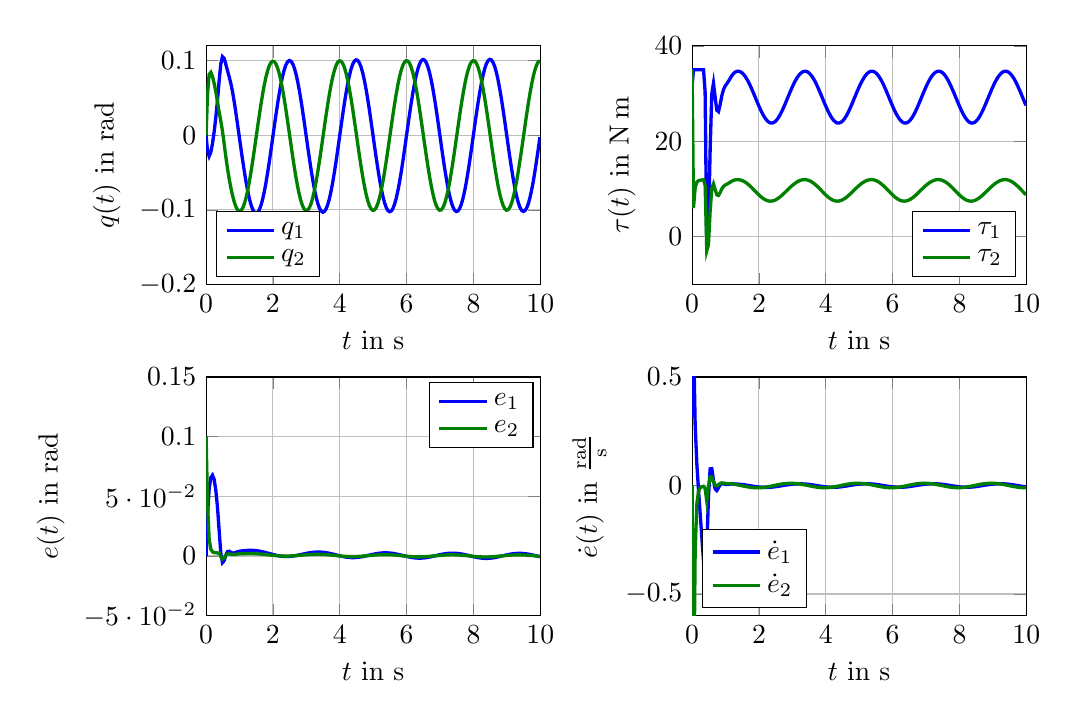
\begin{tikzpicture}

\begin{axis}[%
width=0.35\textwidth,
height=0.25\textwidth,
scale only axis,
xmin=0,
xmax=10,
xlabel={$t$ in $\mathrm{s}$},
xmajorgrids,
ymin=-0.2,
ymax=0.12,
ylabel={$q(t)$ in $\mathrm{rad}$},
ymajorgrids,
name=plot1,
legend style={at={(0.03,0.03)},anchor=south west,draw=black,fill=white,legend cell align=left}
]
\addplot [
color=blue,
solid,
line width=1.2pt
]
table[row sep=crcr]{
0 0\\
0.0417893587846563 -0.020710577574311\\
0.0917893587846563 -0.0280282126130773\\
0.141789358784656 -0.0225865531201604\\
0.191789358784656 -0.0110353318349534\\
0.241789358784656 0.00477572140189046\\
0.291789358784657 0.0242742746864054\\
0.341789358784657 0.0472225885256067\\
0.38992934588091 0.0724254125736438\\
0.43992934588091 0.0956802377166689\\
0.48992934588091 0.105494374509296\\
0.53992934588091 0.103199380733219\\
0.58992934588091 0.0953966085244067\\
0.63992934588091 0.0869052451962601\\
0.68992934588091 0.0787442315087428\\
0.73992934588091 0.0697617292918348\\
0.78992934588091 0.0587968488653107\\
0.839929345880911 0.0456448794349127\\
0.889929345880911 0.0308633759537559\\
0.939929345880911 0.0152016499286962\\
0.989929345880911 -0.000759029560558919\\
1.03992934588091 -0.0166411321668304\\
1.0899293458809 -0.0321491781085752\\
1.1399293458809 -0.046967377322412\\
1.18992934588089 -0.060739830028289\\
1.23992934588088 -0.0731053312417094\\
1.28992934588088 -0.0837380173983353\\
1.33992934588087 -0.0923684688244291\\
1.38992934588087 -0.0987867016010827\\
1.43992934588086 -0.102838944094995\\
1.48992934588086 -0.104426588575331\\
1.53992934588085 -0.103508556000904\\
1.58992934588085 -0.100104365834193\\
1.63992934588084 -0.094295278530796\\
1.68992934588083 -0.0862226610964832\\
1.73992934588083 -0.0760840892974102\\
1.78992934588082 -0.0641280046379346\\
1.83992934588082 -0.0506474130706824\\
1.88992934588081 -0.0359727458208312\\
1.93992934588081 -0.0204638796846126\\
1.9899293458808 -0.00450139002532948\\
2.0399293458808 0.011522770128872\\
2.08992934588079 0.0272149057758646\\
2.13992934588079 0.0421892685273572\\
2.18992934588078 0.056077559930848\\
2.23992934588077 0.0685380302585657\\
2.28992934588077 0.0792639597603464\\
2.33992934588076 0.0879913112111772\\
2.38992934588076 0.0945053503484382\\
2.43992934588075 0.098646049543536\\
2.48992934588075 0.100312119584184\\
2.53992934588074 0.0994635523319812\\
2.58992934588074 0.0961226007894618\\
2.63992934588073 0.0903731705935275\\
2.68992934588072 0.0823586457756343\\
2.73992934588072 0.0722782189336155\\
2.78992934588071 0.0603818387318243\\
2.83992934588071 0.0469639234059053\\
2.8899293458807 0.0323560163454375\\
2.9399293458807 0.0169185788485573\\
2.98992934588069 0.00103212689784127\\
3.03992934588069 -0.0149120749588736\\
3.08992934588068 -0.0305215470064055\\
3.13992934588068 -0.0454121391621859\\
3.18992934588067 -0.0592173725506398\\
3.23992934588066 -0.0715973659640755\\
3.28992934588066 -0.0822471401915821\\
3.33992934588065 -0.0909041012957229\\
3.38992934588065 -0.097354516538934\\
3.43992934588064 -0.101438814999988\\
3.48992934588064 -0.103055569764055\\
3.53992934588063 -0.102164050037483\\
3.58992934588063 -0.0987852689097281\\
3.63992934588062 -0.0930014941790653\\
3.68992934588061 -0.0849542334028409\\
3.73992934588061 -0.0748407475080046\\
3.7899293458806 -0.0629091873888753\\
3.8399293458806 -0.0494524829561704\\
3.88992934588059 -0.034801142961436\\
3.93992934588059 -0.0193151464111166\\
3.98992934588058 -0.003375123090251\\
4.03992934588059 0.0126269673206705\\
4.08992934588061 0.0282974397180845\\
4.13992934588063 0.043250548273409\\
4.18992934588064 0.057117984891161\\
4.23992934588066 0.0695579845412594\\
4.28992934588068 0.0802638136167077\\
4.33992934588069 0.0889714251252938\\
4.38992934588071 0.0954660781195264\\
4.43992934588073 0.0995877394795549\\
4.48992934588074 0.101235114696056\\
4.53992934588076 0.10036819058129\\
4.58992934588078 0.0970092158009235\\
4.63992934588079 0.0912420926739412\\
4.68992934588081 0.0832102029147098\\
4.73992934588083 0.0731127375783806\\
4.78992934588084 0.0611996442899133\\
4.83992934588086 0.0477653405142651\\
4.88992934588088 0.0331413689406713\\
4.93992934588089 0.0176881900488717\\
4.98992934588091 0.00178631869566272\\
5.03992934588093 -0.014172982183489\\
5.08992934588094 -0.0297972351220276\\
5.13992934588096 -0.0447022930282929\\
5.18992934588098 -0.0585216808180883\\
5.23992934588099 -0.070915521888936\\
5.28992934588101 -0.0815788424233357\\
5.33992934588103 -0.0902490546068338\\
5.38992934588104 -0.0967124324685993\\
5.43992934588106 -0.100809412390984\\
5.48992934588108 -0.102438575178404\\
5.53992934588109 -0.101559198043971\\
5.58992934588111 -0.0981923022436013\\
5.63992934588113 -0.0924201637807865\\
5.68992934588114 -0.0843842983481797\\
5.73992934588116 -0.0742819748454986\\
5.78992934588118 -0.0623613519027305\\
5.83992934588119 -0.0489153668729838\\
5.88992934588121 -0.0342745356179661\\
5.93992934588123 -0.0187988438980689\\
5.98992934588124 -0.00286892788410694\\
6.03992934588126 0.0131232467289932\\
6.08992934588128 0.0287839891922324\\
6.13992934588129 0.0437275483958819\\
6.18992934588131 0.0575856113233418\\
6.23992934588133 0.0700164083820282\\
6.28992934588134 0.0807132017641637\\
6.33992934588136 0.0894119406467787\\
6.38992934588138 0.0958978806345092\\
6.43992934588139 0.100010985557804\\
6.48992934588141 0.101649958269951\\
6.53992934588143 0.10077478336644\\
6.58992934588145 0.0974077077141801\\
6.63992934588146 0.0916326322332633\\
6.68992934588148 0.0835929376021608\\
6.7399293458815 0.0734878141465564\\
6.78992934588151 0.0615672089937138\\
6.83992934588153 0.048125539254022\\
6.88992934588155 0.033494347308631\\
6.93992934588156 0.0180340932779811\\
6.98992934588158 0.00212529151647792\\
7.0399293458816 -0.0138407957660394\\
7.08992934588161 -0.0294716921159381\\
7.13992934588163 -0.0443832517871653\\
7.18992934588165 -0.0582090013996349\\
7.23992934588166 -0.0706090664202221\\
7.28992934588168 -0.0812784754552124\\
7.3399293458817 -0.0899546434422533\\
7.38992934588171 -0.0964238474522277\\
7.43992934588173 -0.100526527150559\\
7.48992934588175 -0.102161266811515\\
7.53992934588176 -0.101287347247241\\
7.58992934588178 -0.0979257933844389\\
7.6399293458818 -0.0921588849148075\\
7.68992934588181 -0.084128141187771\\
7.73992934588183 -0.074030834686729\\
7.78992934588185 -0.0621151275187326\\
7.83992934588186 -0.0486739603820807\\
7.88992934588188 -0.034037852334295\\
7.9399293458819 -0.0185667921714336\\
7.98992934588191 -0.00264141893446717\\
8.03992934588189 0.0133462989784448\\
8.08992934588187 0.0290026682809282\\
8.13992934588184 0.0439419354896162\\
8.18992934588181 0.0577957853760794\\
8.23992934588178 0.0702224462970633\\
8.28992934588176 0.0809151785566673\\
8.33992934588173 0.0896099296100752\\
8.3899293458817 0.0960919535121335\\
8.43992934588167 0.100201212722435\\
8.48992934588165 0.101836408908704\\
8.53992934588162 0.100957525669902\\
8.58992934588159 0.0975868090642837\\
8.63992934588156 0.0918081593830146\\
8.68992934588153 0.0837649568388042\\
8.73992934588151 0.0736563914293237\\
8.78992934588148 0.0617324100580237\\
8.83992934588145 0.0482874296758393\\
8.88992934588142 0.0336529925253895\\
8.9399293458814 0.018189558565591\\
8.98992934588137 0.00227764192503423\\
9.03992934588134 -0.0136914955125768\\
9.08992934588131 -0.0293253777488627\\
9.13992934588128 -0.0442398596425494\\
9.18992934588126 -0.0580684685794639\\
9.23992934588123 -0.0704713309565624\\
9.2899293458812 -0.0811434764695231\\
9.33992934588117 -0.0898223212929598\\
9.38992934588115 -0.0962941438648999\\
9.43992934588112 -0.100399385326399\\
9.48992934588109 -0.102036631511313\\
9.53992934588106 -0.101165164849437\\
9.58992934588104 -0.0978060119173746\\
9.63992934588101 -0.0920414540645511\\
9.68992934588098 -0.0840130122839824\\
9.73992934588095 -0.0739179606698018\\
9.78992934588092 -0.0620044628918644\\
9.8399293458809 -0.048565461151993\\
9.88992934588087 -0.0339314759440863\\
9.93992934588084 -0.0184624974285923\\
9.98992934588081 -0.0025391659364765\\
};
\addlegendentry{$q_1$};

\addplot [
color=green!50!black,
solid,
line width=1.2pt
]
table[row sep=crcr]{
0 0\\
0.0417893587846563 0.0541897747095662\\
0.0917893587846563 0.0817864000262958\\
0.141789358784656 0.0844811113802557\\
0.191789358784656 0.078899325516466\\
0.241789358784656 0.0696620720805113\\
0.291789358784657 0.0582008846527589\\
0.341789358784657 0.0451218130036955\\
0.38992934588091 0.0313998762506606\\
0.43992934588091 0.0193534500280922\\
0.48992934588091 0.0057884454878286\\
0.53992934588091 -0.0108980262848867\\
0.58992934588091 -0.0282852848941022\\
0.63992934588091 -0.0442192321690119\\
0.68992934588091 -0.0580241664016155\\
0.73992934588091 -0.069934355579966\\
0.78992934588091 -0.0802325059532825\\
0.839929345880911 -0.0888627187443021\\
0.889929345880911 -0.0955163633824564\\
0.939929345880911 -0.099870554023041\\
0.989929345880911 -0.101737386439194\\
1.03992934588091 -0.101077467559925\\
1.0899293458809 -0.0979467410490464\\
1.1399293458809 -0.092449736147588\\
1.18992934588089 -0.0847255465507898\\
1.23992934588088 -0.0749551641545504\\
1.28992934588088 -0.0633701739156066\\
1.33992934588087 -0.0502524861172338\\
1.38992934588087 -0.0359259051640063\\
1.43992934588086 -0.0207446946896944\\
1.48992934588086 -0.00508286534468728\\
1.53992934588085 0.0106750465799447\\
1.58992934588085 0.0261425797943643\\
1.63992934588084 0.0409401751024088\\
1.68992934588083 0.0547043519333933\\
1.73992934588083 0.0670968134427046\\
1.78992934588082 0.0778129593986603\\
1.83992934588082 0.086589453238286\\
1.88992934588081 0.0932106742844176\\
1.93992934588081 0.0975139720858763\\
1.9899293458808 0.0993936450660065\\
2.0399293458808 0.0988035533897191\\
2.08992934588079 0.0957582864029471\\
2.13992934588079 0.0903328411133682\\
2.18992934588078 0.0826608143495966\\
2.23992934588077 0.0729311537977198\\
2.28992934588077 0.0613835479997069\\
2.33992934588076 0.0483025650723291\\
2.38992934588076 0.0340106777028343\\
2.43992934588075 0.0188603390585609\\
2.48992934588075 0.0032252996680188\\
2.53992934588074 -0.0125086226223707\\
2.58992934588074 -0.0279530903292201\\
2.63992934588073 -0.0427268710825616\\
2.68992934588072 -0.0564652942428899\\
2.73992934588072 -0.0688292967680241\\
2.78992934588071 -0.0795138258388198\\
2.83992934588071 -0.0882553833027815\\
2.8899293458807 -0.0948385213003577\\
2.9399293458807 -0.0991011283149399\\
2.98992934588069 -0.10093837880877\\
3.03992934588069 -0.100305255949128\\
3.08992934588068 -0.0972175941952012\\
3.13992934588068 -0.0917516254881179\\
3.18992934588067 -0.0840420485866996\\
3.23992934588066 -0.0742786751591866\\
3.28992934588066 -0.0627017382550694\\
3.33992934588065 -0.0495959785515695\\
3.38992934588065 -0.0352836511284513\\
3.43992934588064 -0.0201166202320935\\
3.48992934588064 -0.00446773116727634\\
3.53992934588063 0.0112783334350808\\
3.58992934588063 0.0267344918560826\\
3.63992934588062 0.0415207660154328\\
3.68992934588061 0.0552736154156329\\
3.73992934588061 0.0676548719173502\\
3.7899293458806 0.0783600541771584\\
3.8399293458806 0.0871258559649399\\
3.88992934588059 0.0937366236081396\\
3.93992934588059 0.0980296636651203\\
3.98992934588058 0.0998992516074672\\
4.03992934588059 0.099299244727811\\
4.08992934588061 0.0962442366673435\\
4.13992934588063 0.0908092259727151\\
4.18992934588064 0.083127806188002\\
4.23992934588066 0.0733889195494393\\
4.28992934588068 0.0618322498810768\\
4.33992934588069 0.0487423623651956\\
4.38992934588071 0.0344417280761708\\
4.43992934588073 0.0192827990642847\\
4.48992934588074 0.00363932478326833\\
4.53992934588076 -0.0121028779656504\\
4.58992934588078 -0.0275554725528825\\
4.63992934588079 -0.0423372271709818\\
4.68992934588081 -0.056083471482301\\
4.73992934588083 -0.0684551425979246\\
4.78992934588084 -0.0791471878281578\\
4.83992934588086 -0.0878961092291139\\
4.88992934588088 -0.094486459309753\\
4.93992934588089 -0.0987561271511966\\
4.98992934588091 -0.100600288105604\\
5.03992934588093 -0.0999739265756378\\
5.08992934588094 -0.0968928786386532\\
5.13992934588096 -0.0914333782543244\\
5.18992934588098 -0.0837301265986356\\
5.23992934588099 -0.0739729381376161\\
5.28992934588101 -0.0624020490687466\\
5.33992934588103 -0.0493022035277976\\
5.38992934588104 -0.0349956603171489\\
5.43992934588106 -0.0198342876182863\\
5.48992934588108 -0.00419093482839453\\
5.53992934588109 0.0115497112293911\\
5.58992934588111 0.0270005646026468\\
5.63992934588113 0.0417816429944403\\
5.68992934588114 0.0555294017640238\\
5.73992934588116 0.0679056687554086\\
5.78992934588118 0.0786059587833029\\
5.83992934588119 0.087366961991944\\
5.88992934588121 0.0939730213324093\\
5.93992934588123 0.0982614402594223\\
5.98992934588124 0.10012649142688\\
6.03992934588126 0.099522029598828\\
6.08992934588128 0.0964626461710741\\
6.13992934588129 0.0910233377149341\\
6.18992934588131 0.0833376960511877\\
6.23992934588133 0.0735946619245348\\
6.28992934588134 0.0620339178791206\\
6.33992934588136 0.0489400280107565\\
6.38992934588138 0.0346354624853713\\
6.43992934588139 0.0194726726099751\\
6.48992934588141 0.00382540724867672\\
6.53992934588143 -0.0119205172454076\\
6.58992934588145 -0.0273767645642489\\
6.63992934588146 -0.0421621031151153\\
6.68992934588148 -0.0559118626938506\\
6.7399293458815 -0.0682869804954364\\
6.78992934588151 -0.0789824039010204\\
6.83992934588153 -0.0877346350638525\\
6.88992934588155 -0.0943282266557263\\
6.93992934588156 -0.0986010680228469\\
6.98992934588158 -0.100448334915828\\
7.0399293458816 -0.0998250122929501\\
7.08992934588161 -0.0967469369598074\\
7.13992934588163 -0.0912903437839087\\
7.18992934588165 -0.083589935027742\\
7.23992934588166 -0.073835526414724\\
7.28992934588168 -0.0622673555572234\\
7.3399293458817 -0.0491701681456692\\
7.38992934588171 -0.0348662246559113\\
7.43992934588173 -0.01970739503844\\
7.48992934588175 -0.00406653053011454\\
7.53992934588176 0.0116716801614355\\
7.58992934588178 0.0271201491807613\\
7.6399293458818 0.0418988923355342\\
7.68992934588181 0.0556443631226391\\
7.73992934588183 0.0680183875806721\\
7.78992934588185 0.0787164787975444\\
7.83992934588186 0.0874753252879342\\
7.88992934588188 0.0940792684854448\\
7.9399293458819 0.0983656104499385\\
7.98992934588191 0.100228622568993\\
8.03992934588189 0.0996221584702833\\
8.08992934588187 0.0965608085405242\\
8.13992934588184 0.0911195684632959\\
8.18992934588181 0.0834320292848979\\
8.23992934588178 0.0736871310796843\\
8.28992934588176 0.0621245558165385\\
8.33992934588173 0.0490288671029162\\
8.3899293458817 0.0347225346963748\\
8.43992934588167 0.0195580095697678\\
8.48992934588165 0.00390904032209041\\
8.53992934588162 -0.0118385568950598\\
8.58992934588159 -0.0272964459182926\\
8.63992934588156 -0.0420833952514843\\
8.68992934588153 -0.0558347347505669\\
8.73992934588151 -0.0682114016483008\\
8.78992934588148 -0.0789083433577257\\
8.83992934588145 -0.0876620620757808\\
8.88992934588142 -0.09425711054746\\
8.9399293458814 -0.0985313782381118\\
8.98992934588137 -0.100380041077428\\
9.03992934588134 -0.0997580842734036\\
9.08992934588131 -0.0966813449589314\\
9.13992934588128 -0.091226058409546\\
9.18992934588126 -0.0835269273760727\\
9.23992934588123 -0.0737737681470801\\
9.2899293458812 -0.0622068189708874\\
9.33992934588117 -0.0491108262367044\\
9.38992934588115 -0.0348080511725682\\
9.43992934588112 -0.0196503645240987\\
9.48992934588109 -0.00401061835504852\\
9.53992934588106 0.011726497779918\\
9.58992934588104 0.0271738951699941\\
9.63992934588101 0.0419515887709305\\
9.68992934588098 0.055696031242546\\
9.73992934588095 0.0680690478119789\\
9.78992934588092 0.0787661507910289\\
9.8399293458809 0.0875240279619759\\
9.88992934588087 0.0941270200764101\\
9.93992934588084 0.0984124285672951\\
9.98992934588081 0.100274524253087\\
};
\addlegendentry{$q_2$};

\end{axis}

\begin{axis}[%
width=0.35\textwidth,
height=0.25\textwidth,
scale only axis,
xmin=0,
xmax=10,
xlabel={$t$ in $\mathrm{s}$},
xmajorgrids,
ymin=-0.05,
ymax=0.15,
ylabel={$e(t)$ in $\mathrm{rad}$},
ymajorgrids,
name=plot3,
at=(plot1.below south west),
anchor=above north west,
legend style={draw=black,fill=white,legend cell align=left}
]
\addplot [
color=blue,
solid,
line width=1.2pt
]
table[row sep=crcr]{
0 0\\
0.0417893587846563 0.0338014109347357\\
0.0917893587846563 0.0564667025506029\\
0.141789358784656 0.0656724496305881\\
0.191789358784656 0.0677077171523041\\
0.241789358784656 0.0640876905110066\\
0.291789358784657 0.0550845180761813\\
0.341789358784657 0.0406775082321217\\
0.38992934588091 0.02165514315827\\
0.43992934588091 0.00254432569967858\\
0.48992934588091 -0.00554441814846106\\
0.53992934588091 -0.00398513106838863\\
0.58992934588091 0.000638950344455116\\
0.63992934588091 0.00358690869353499\\
0.68992934588091 0.00397630024697854\\
0.73992934588091 0.00315032630428161\\
0.78992934588091 0.00251139378118523\\
0.839929345880911 0.0025499378576142\\
0.889929345880911 0.00303129963363163\\
0.939929345880911 0.00355828455061159\\
0.989929345880911 0.00392229108425333\\
1.03992934588091 0.00412983073793634\\
1.0899293458809 0.00427138349090126\\
1.1399293458809 0.00440953334054096\\
1.18992934588089 0.00454985204244086\\
1.23992934588088 0.00466680299374071\\
1.28992934588088 0.00473612258816374\\
1.33992934588087 0.00474849629453751\\
1.38992934588087 0.00470614586917333\\
1.43992934588086 0.00461438067865064\\
1.48992934588086 0.00447663221449755\\
1.53992934588085 0.00429430633607084\\
1.58992934588085 0.00406880696532563\\
1.63992934588084 0.00380312464099146\\
1.68992934588083 0.00350212934074851\\
1.73992934588083 0.00317203370127629\\
1.78992934588082 0.00281976199141711\\
1.83992934588082 0.00245259577813003\\
1.88992934588081 0.00207807023341475\\
1.93992934588081 0.00170394520527298\\
1.9899293458808 0.00133812850160084\\
2.0399293458808 0.000988531299987756\\
2.08992934588079 0.00066288884177616\\
2.13992934588079 0.000368575454482482\\
2.18992934588078 0.0001124180549716\\
2.23992934588077 -9.95020106222128e-05\\
2.28992934588077 -0.000262064950195998\\
2.33992934588076 -0.000371338681302236\\
2.38992934588076 -0.000424794616540561\\
2.43992934588075 -0.000421486127197779\\
2.48992934588075 -0.000362163223350781\\
2.53992934588074 -0.000249302667144069\\
2.58992934588074 -8.70419205847017e-05\\
2.63992934588073 0.000118983296291647\\
2.68992934588072 0.000361885980119742\\
2.73992934588072 0.000633836662542048\\
2.78992934588071 0.000926403914720549\\
2.83992934588071 0.00123089388667724\\
2.8899293458807 0.00153865924201139\\
2.9399293458807 0.0018413556308164\\
2.98992934588069 0.00213113462592192\\
3.03992934588069 0.00240077353004815\\
3.08992934588068 0.00264375238879792\\
3.13992934588068 0.00285429518037759\\
3.18992934588067 0.00302739456484882\\
3.23992934588066 0.00315883771615724\\
3.28992934588066 0.00324524538145295\\
3.33992934588065 0.00328412876586465\\
3.38992934588065 0.00327396080704813\\
3.43992934588064 0.00321425158365587\\
3.48992934588064 0.0031056134032237\\
3.53992934588063 0.00294980037264185\\
3.58992934588063 0.00274971004084133\\
3.63992934588062 0.00250934028923142\\
3.68992934588061 0.00223370164706738\\
3.73992934588061 0.0019286919118234\\
3.7899293458806 0.00160094474230309\\
3.8399293458806 0.00125766566355744\\
3.88992934588059 0.000906467373954487\\
3.93992934588059 0.000555211931709099\\
3.98992934588058 0.000211861566453175\\
4.03992934588059 -0.000115665891874015\\
4.08992934588061 -0.000419645100498224\\
4.13992934588063 -0.000692704291614291\\
4.18992934588064 -0.000928006905376873\\
4.23992934588066 -0.00111945629334199\\
4.28992934588068 -0.00126191880657504\\
4.33992934588069 -0.00135145259542939\\
4.38992934588071 -0.00138552238763388\\
4.43992934588073 -0.0013631760632182\\
4.48992934588074 -0.00128515833522359\\
4.53992934588076 -0.00115394091645379\\
4.58992934588078 -0.000973656932050024\\
4.63992934588079 -0.000749938784130488\\
4.68992934588081 -0.000489671158970806\\
4.73992934588083 -0.000200681982246279\\
4.78992934588084 0.000108598356599238\\
4.83992934588086 0.000429476778275636\\
4.88992934588088 0.000753306646726203\\
4.93992934588089 0.00107174443044124\\
4.98992934588091 0.00137694282803178\\
5.03992934588093 0.00166168075458856\\
5.08992934588094 0.00191944050434073\\
5.13992934588096 0.00214444904640335\\
5.18992934588098 0.00233170283221726\\
5.23992934588099 0.0024769936409422\\
5.28992934588101 0.00257694761313873\\
5.33992934588103 0.00262908207691891\\
5.38992934588104 0.00263187673667117\\
5.43992934588106 0.00258484897462752\\
5.48992934588108 0.00248861881756773\\
5.53992934588109 0.00234494837914809\\
5.58992934588111 0.00215674337475708\\
5.63992934588113 0.0019280098910204\\
5.68992934588114 0.00166376659249974\\
5.73992934588116 0.00136991924943596\\
5.78992934588118 0.00105310925630082\\
5.83992934588119 0.000720549580534843\\
5.88992934588121 0.000379860030667409\\
5.93992934588123 3.89094188588159e-05\\
5.98992934588124 -0.000294333639482651\\
6.03992934588126 -0.000611945299988712\\
6.08992934588128 -0.000906194574444706\\
6.13992934588129 -0.00116970441389721\\
6.18992934588131 -0.00139563333738411\\
6.23992934588133 -0.00157788013395774\\
6.28992934588134 -0.00171130695390243\\
6.33992934588136 -0.00179196811681309\\
6.38992934588138 -0.00181732490254552\\
6.43992934588139 -0.00178642214142832\\
6.48992934588141 -0.00170000190911185\\
6.53992934588143 -0.00156053370162998\\
6.58992934588145 -0.00137214884536507\\
6.63992934588146 -0.00114047834354195\\
6.68992934588148 -0.000872405846539734\\
6.7399293458815 -0.0005757585505657\\
6.78992934588151 -0.000258966347366975\\
6.83992934588153 6.92780383347927e-05\\
6.88992934588155 0.000400328278569104\\
6.93992934588156 0.000725841201125628\\
6.98992934588158 0.00103797000700693\\
7.0399293458816 0.00132949433693067\\
7.08992934588161 0.00159389749804973\\
7.13992934588163 0.00182540780508579\\
7.18992934588165 0.00201902341359051\\
7.23992934588166 0.00217053817207526\\
7.28992934588168 0.00227658064488689\\
7.3399293458817 0.00233467091223719\\
7.38992934588171 0.00234329172022855\\
7.43992934588173 0.00230196373416312\\
7.48992934588175 0.00221131045067249\\
7.53992934588176 0.00207309758244399\\
7.58992934588178 0.00189023451565302\\
7.6399293458818 0.00166673102513068\\
7.68992934588181 0.00140760943220894\\
7.73992934588183 0.00111877909081004\\
7.78992934588185 0.000806884872468792\\
7.83992934588186 0.000479143089815677\\
7.88992934588188 0.000143176747193836\\
7.9399293458819 -0.000193142307570223\\
7.98992934588191 -0.000521842588912587\\
8.03992934588189 -0.000834997549242966\\
8.08992934588187 -0.00112487366296279\\
8.13992934588184 -0.00138409150747688\\
8.18992934588181 -0.00160580738999188\\
8.23992934588178 -0.00178391804888871\\
8.28992934588176 -0.00191328374632684\\
8.33992934588173 -0.00198995708005413\\
8.3899293458817 -0.0020113977801355\\
8.43992934588167 -0.00197664930604274\\
8.48992934588165 -0.00188645254786186\\
8.53992934588162 -0.00174327600509884\\
8.58992934588159 -0.00155125019548132\\
8.63992934588156 -0.00131600549330647\\
8.68992934588153 -0.00104442508319302\\
8.73992934588151 -0.000744335833335483\\
8.78992934588148 -0.000424167411668647\\
8.83992934588145 -9.26123834610326e-05\\
8.88992934588142 0.000241683061846396\\
8.9399293458814 0.000570375913567102\\
8.98992934588137 0.000885619598516688\\
9.03992934588134 0.00118019408354766\\
9.08992934588131 0.00144758313106445\\
9.13992934588128 0.00168201566056771\\
9.18992934588126 0.00187849059352035\\
9.23992934588123 0.00203280270851482\\
9.2899293458812 0.00214158165928928\\
9.33992934588117 0.00220234876302264\\
9.38992934588115 0.00221358813296095\\
9.43992934588112 0.00217482191003918\\
9.48992934588109 0.00208667515047674\\
9.53992934588106 0.00195091518461242\\
9.58992934588104 0.00177045304852369\\
9.63992934588101 0.00154930017476895\\
9.68992934588098 0.00129248052827349\\
9.73992934588095 0.00100590507369443\\
9.78992934588092 0.000696220245371894\\
9.8399293458809 0.000370643859462151\\
9.88992934588087 3.68003566865449e-05\\
9.93992934588084 -0.000297437050736839\\
9.98992934588081 -0.000624095587248433\\
};
\addlegendentry{$e_1$};

\addplot [
color=green!50!black,
solid,
line width=1.2pt
]
table[row sep=crcr]{
0 0.1\\
0.0417893587846563 0.044949672948415\\
0.0917893587846563 0.0140846190048653\\
0.141789358784656 0.00576081635786783\\
0.191789358784656 0.00349145517192005\\
0.241789358784656 0.00284882709826505\\
0.291789358784657 0.00264467402874898\\
0.341789358784657 0.00256018559097329\\
0.38992934588091 0.00249479933672711\\
0.43992934588091 -0.000593515548784361\\
0.48992934588091 -0.00262518396413406\\
0.53992934588091 -0.00161327514400854\\
0.58992934588091 0.000407490276425389\\
0.63992934588091 0.00166138818713657\\
0.68992934588091 0.00183418841576195\\
0.73992934588091 0.00149582733199126\\
0.78992934588091 0.00123061114310491\\
0.839929345880911 0.00124274621440482\\
0.889929345880911 0.00143580765054253\\
0.939929345880911 0.00164599060669343\\
0.989929345880911 0.00178743007835971\\
1.03992934588091 0.00186321789509437\\
1.0899293458809 0.0019111821801837\\
1.1399293458809 0.00195758225779084\\
1.18992934588089 0.00200501479506489\\
1.23992934588088 0.00204310855842839\\
1.28992934588088 0.00206193126910275\\
1.33992934588087 0.00205766882469656\\
1.38992934588087 0.00203122957660614\\
1.43992934588086 0.00198476021037164\\
1.48992934588086 0.00191960382097595\\
1.53992934588085 0.0018362548489321\\
1.58992934588085 0.00173521482329305\\
1.63992934588084 0.00161766887944648\\
1.68992934588083 0.00148562605244053\\
1.73992934588083 0.00134171480525142\\
1.78992934588082 0.00118893541150059\\
1.83992934588082 0.00103051929159727\\
1.88992934588081 0.000869881447485912\\
1.93992934588081 0.00071059133046518\\
1.9899293458808 0.000556311294826889\\
2.0399293458808 0.000410696275115932\\
2.08992934588079 0.00027727246592521\\
2.13992934588079 0.00015931277644364\\
2.18992934588078 5.97174061476996e-05\\
2.23992934588077 -1.90982015741276e-05\\
2.28992934588077 -7.53053531757156e-05\\
2.33992934588076 -0.00010774777976158\\
2.38992934588076 -0.000116002115401602\\
2.43992934588075 -0.000100404579204329\\
2.48992934588075 -6.2038144272923e-05\\
2.53992934588074 -2.67880647193165e-06\\
2.58992934588074 7.52957115959241e-05\\
2.63992934588073 0.000169027100737504\\
2.68992934588072 0.000275316257084567\\
2.73992934588072 0.00039076852009326\\
2.78992934588071 0.000511931028680107\\
2.83992934588071 0.000635410772914929\\
2.8899293458807 0.000757965568465899\\
2.9399293458807 0.000876564898604965\\
2.98992934588069 0.000988422447937926\\
3.03992934588069 0.00109100628428899\\
3.08992934588068 0.00118203532631921\\
3.13992934588068 0.00125947159829133\\
3.18992934588067 0.00132151683093579\\
3.23992934588066 0.00136661956301726\\
3.28992934588066 0.00139349560851099\\
3.33992934588065 0.00140116125897166\\
3.38992934588065 0.00138897554098598\\
3.43992934588064 0.00135668575270291\\
3.48992934588064 0.00130446964349592\\
3.53992934588063 0.00123296799372758\\
3.58992934588063 0.00114330276150825\\
3.63992934588062 0.00103707796635998\\
3.68992934588061 0.000916362570143783\\
3.73992934588061 0.000783656330555479\\
3.7899293458806 0.000641840632960036\\
3.8399293458806 0.000494116564910038\\
3.88992934588059 0.000343932123740412\\
3.93992934588059 0.000194899751208191\\
3.98992934588058 5.07047533639532e-05\\
4.03992934588059 -8.49950629680379e-05\\
4.08992934588061 -0.000208677798455389\\
4.13992934588063 -0.000317072082882078\\
4.18992934588064 -0.000407274432233623\\
4.23992934588066 -0.00047686395326911\\
4.28992934588068 -0.000524007234522825\\
4.33992934588069 -0.000547545072608978\\
4.38992934588071 -0.000547052488723977\\
4.43992934588073 -0.000522864584920207\\
4.48992934588074 -0.000476063259521457\\
4.53992934588076 -0.000408423463198072\\
4.58992934588078 -0.000322322064754063\\
4.63992934588079 -0.000220616810860261\\
4.68992934588081 -0.000106506503526546\\
4.73992934588083 1.66143499690102e-05\\
4.78992934588084 0.000145293017993015\\
4.83992934588086 0.000276136699224272\\
4.88992934588088 0.000405903577842731\\
4.93992934588089 0.000531563734850096\\
4.98992934588091 0.000650331744769278\\
5.03992934588093 0.00075967691080793\\
5.08992934588094 0.000857319769794251\\
5.13992934588096 0.000941224364535975\\
5.18992934588098 0.00100959484292616\\
5.23992934588099 0.00106088254151755\\
5.28992934588101 0.00109380642227552\\
5.33992934588103 0.00110738623530273\\
5.38992934588104 0.00110098472980091\\
5.43992934588106 0.00107435313902483\\
5.48992934588108 0.00102767330475257\\
5.53992934588109 0.000961590199561411\\
5.58992934588111 0.000877230015090543\\
5.63992934588113 0.000776200987496659\\
5.68992934588114 0.000660576221890578\\
5.73992934588116 0.000532859492623369\\
5.78992934588118 0.000395936026926239\\
5.83992934588119 0.000253010537996187\\
5.88992934588121 0.000107534399536591\\
5.93992934588123 -3.68768430561162e-05\\
5.98992934588124 -0.000176535066042177\\
6.03992934588126 -0.000307779934011224\\
6.08992934588128 -0.000427087302244389\\
6.13992934588129 -0.000531183825190393\\
6.18992934588131 -0.00061716429553714\\
6.23992934588133 -0.000682606328508223\\
6.28992934588134 -0.000725675232732363\\
6.33992934588136 -0.000745210718353768\\
6.38992934588138 -0.000740786898121862\\
6.43992934588139 -0.000712738130816824\\
6.48992934588141 -0.000662145725139503\\
6.53992934588143 -0.000590784183649183\\
6.58992934588145 -0.000501030053589105\\
6.63992934588146 -0.000395740866916822\\
6.68992934588148 -0.000278115292150431\\
6.7399293458815 -0.000151547752672246\\
6.78992934588151 -1.94909092729456e-05\\
6.83992934588153 0.000114662533861692\\
6.88992934588155 0.000247670923744864\\
6.93992934588156 0.000376504606461006\\
6.98992934588158 0.000498378554986564\\
7.0399293458816 0.000610762628146522\\
7.08992934588161 0.000711378091006964\\
7.13992934588163 0.000798189894209655\\
7.18992934588165 0.000869403272150293\\
7.23992934588166 0.000923470818769229\\
7.28992934588168 0.000959112910917909\\
7.3399293458817 0.000975350853358314\\
7.38992934588171 0.000971549068760506\\
7.43992934588173 0.000947460559384716\\
7.48992934588175 0.000903269006682058\\
7.53992934588176 0.000839621267725264\\
7.58992934588178 0.000757645437177389\\
7.6399293458818 0.000658951646592743\\
7.68992934588181 0.000545614863448909\\
7.73992934588183 0.000420140667513003\\
7.78992934588185 0.000285416012813469\\
7.83992934588186 0.00014464724210711\\
7.88992934588188 1.28724657222357e-06\\
7.9399293458819 -0.00014104703353289\\
7.98992934588191 -0.000278666208148842\\
8.03992934588189 -0.00040790880549145\\
8.08992934588187 -0.000525249671746081\\
8.13992934588184 -0.000627414573624932\\
8.18992934588181 -0.000711497529335553\\
8.23992934588178 -0.000775075483755466\\
8.28992934588176 -0.000816313170252408\\
8.33992934588173 -0.000834049810614322\\
8.3899293458817 -0.000827859109220647\\
8.43992934588167 -0.000798075090694989\\
8.48992934588165 -0.000745778798626667\\
8.53992934588162 -0.000672744534055853\\
8.58992934588159 -0.000581348699589052\\
8.63992934588156 -0.000474448730576019\\
8.68992934588153 -0.000355243235448784\\
8.73992934588151 -0.000227126599810404\\
8.78992934588148 -9.35514525613607e-05\\
8.83992934588145 4.20895458018017e-05\\
8.88992934588142 0.000176554815491461\\
8.9399293458814 0.00030681482173571\\
8.98992934588137 0.000430084716588952\\
9.03992934588134 0.000543834608589935\\
9.08992934588131 0.000645786090104836\\
9.13992934588128 0.000733904519800987\\
9.18992934588126 0.000806395620412501\\
9.23992934588123 0.000861712551032151\\
9.2899293458812 0.000898576324463808\\
9.33992934588117 0.000916008944249994\\
9.38992934588115 0.000913375585250217\\
9.43992934588112 0.000890430044854958\\
9.48992934588109 0.00084735683141077\\
9.53992934588106 0.000784803649024904\\
9.58992934588104 0.000703899447720355\\
9.63992934588101 0.000606255210972344\\
9.68992934588098 0.000493946743325674\\
9.73992934588095 0.000369480436005404\\
9.78992934588092 0.000235744019151399\\
9.8399293458809 9.59445679191567e-05\\
9.88992934588087 -4.64643445006185e-05\\
9.93992934588084 -0.000187865150951663\\
9.98992934588081 -0.000324567892253949\\
};
\addlegendentry{$e_2$};

\end{axis}

\begin{axis}[%
width=0.35\textwidth,
height=0.25\textwidth,
scale only axis,
xmin=0,
xmax=10,
xlabel={$t$ in $\mathrm{s}$},
xmajorgrids,
ymin=-0.6,
ymax=0.5,
ylabel={$\dot{e}(t)$ in $\mathrm{\frac{rad}{s}}$},
ymajorgrids,
name=plot2,
at=(plot3.right of south east),
anchor=left of south west,
legend style={at={(0.03,0.03)},anchor=south west,draw=black,fill=white,legend cell align=left}
]
\addplot [
color=blue,
solid,
line width=1.2pt
]
table[row sep=crcr]{
0 0.314159265358979\\
0.0417893587846563 0.691192917375483\\
0.0917893587846563 0.280738259826231\\
0.141789358784656 0.100753004048407\\
0.191789358784656 -0.0211200557834962\\
0.241789358784656 -0.130418198023477\\
0.291789358784657 -0.238549778821761\\
0.341789358784657 -0.347742830136557\\
0.38992934588091 -0.449242867461648\\
0.43992934588091 -0.29266028414525\\
0.48992934588091 -0.053654832533313\\
0.53992934588091 0.0762608074057397\\
0.58992934588091 0.0774216357663689\\
0.63992934588091 0.024051326102188\\
0.68992934588091 -0.0163690427342496\\
0.73992934588091 -0.0234886179454989\\
0.78992934588091 -0.0106850237617682\\
0.839929345880911 0.00299521978517886\\
0.889929345880911 0.00869682902273572\\
0.939929345880911 0.00783514956472758\\
0.989929345880911 0.00530569300280642\\
1.03992934588091 0.00423950554015134\\
1.0899293458809 0.00491502776355413\\
1.1399293458809 0.00618770262193563\\
1.18992934588089 0.00705365007035419\\
1.23992934588088 0.00723090073966731\\
1.28992934588088 0.0069317336664769\\
1.33992934588087 0.00643911451493301\\
1.38992934588087 0.00588089970341509\\
1.43992934588086 0.00523927260417944\\
1.48992934588086 0.00445500368716872\\
1.53992934588085 0.00350301864983565\\
1.58992934588085 0.00240502385434233\\
1.63992934588084 0.00120608832253499\\
1.68992934588083 -4.93642058252974e-05\\
1.73992934588083 -0.00132644650714264\\
1.78992934588082 -0.00259675991598096\\
1.83992934588082 -0.00383261946826019\\
1.88992934588081 -0.00500428272247166\\
1.93992934588081 -0.0060806516456659\\
1.9899293458808 -0.0070313885125699\\
2.0399293458808 -0.00782871066001889\\
2.08992934588079 -0.0084484434821066\\
2.13992934588079 -0.00887074138481614\\
2.18992934588078 -0.00908091666839378\\
2.23992934588077 -0.00907045080394736\\
2.28992934588077 -0.00883795345623581\\
2.33992934588076 -0.00838975757751131\\
2.38992934588076 -0.00773993549157824\\
2.43992934588075 -0.00690966908265037\\
2.48992934588075 -0.00592603252328584\\
2.53992934588074 -0.00482033372492586\\
2.58992934588074 -0.00362621984589606\\
2.63992934588073 -0.00237778539215072\\
2.68992934588072 -0.00110792028001713\\
2.73992934588072 0.000152908599766549\\
2.78992934588071 0.00137733230586762\\
2.83992934588071 0.00254120772725452\\
2.8899293458807 0.00362329942640688\\
2.9399293458807 0.00460469484606474\\
2.98992934588069 0.00546816837141234\\
3.03992934588069 0.00619769881488813\\
3.08992934588068 0.00677829315892625\\
3.13992934588068 0.00719619080048661\\
3.18992934588067 0.00743943462877777\\
3.23992934588066 0.0074987153561894\\
3.28992934588066 0.00736833789167965\\
3.33992934588065 0.00704713262622678\\
3.38992934588065 0.00653914383321103\\
3.43992934588064 0.00585396917444432\\
3.48992934588064 0.00500668963337834\\
3.53992934588063 0.00401740425637689\\
3.58992934588063 0.00291045258250153\\
3.63992934588062 0.00171345431044923\\
3.68992934588061 0.000456310160337897\\
3.73992934588061 -0.000829712536060678\\
3.7899293458806 -0.00211273491923514\\
3.8399293458806 -0.00336085151646481\\
3.88992934588059 -0.00454259540237195\\
3.93992934588059 -0.00562737663700064\\
3.98992934588058 -0.00658600022349365\\
4.03992934588059 -0.00739135063204549\\
4.08992934588061 -0.00801928316585987\\
4.13992934588063 -0.00844969894076264\\
4.18992934588064 -0.00866771407711431\\
4.23992934588066 -0.00866477929615411\\
4.28992934588068 -0.00843957584593358\\
4.33992934588069 -0.00799851593165696\\
4.38992934588071 -0.00735571344434993\\
4.43992934588073 -0.00653236001411209\\
4.48992934588074 -0.00555553161046594\\
4.53992934588076 -0.00445654557045738\\
4.58992934588078 -0.0032690674405059\\
4.63992934588079 -0.0020272129162216\\
4.68992934588081 -0.000763890054121724\\
4.73992934588083 0.000490421533481944\\
4.78992934588084 0.00170834534387326\\
4.83992934588086 0.0028657349509365\\
4.88992934588088 0.00394135539232232\\
4.93992934588089 0.00491629836913055\\
4.98992934588091 0.00577334627246445\\
5.03992934588093 0.00649648927166824\\
5.08992934588094 0.00707074829336596\\
5.13992934588096 0.007482378319706\\
5.18992934588098 0.00771943852328544\\
5.23992934588099 0.00777263575655396\\
5.28992934588101 0.0076362902064685\\
5.33992934588103 0.00730924607810154\\
5.38992934588104 0.00679555951021599\\
5.43992934588106 0.00610483772532051\\
5.48992934588108 0.00525216874956736\\
5.53992934588109 0.00425765608877401\\
5.58992934588111 0.00314564123360968\\
5.63992934588113 0.00194374352293913\\
5.68992934588114 0.000681861294353603\\
5.73992934588116 -0.000608742178603211\\
5.78992934588118 -0.00189619340041136\\
5.83992934588119 -0.00314859320766425\\
5.88992934588121 -0.00433448160473671\\
5.93992934588123 -0.00542327593031583\\
5.98992934588124 -0.0063857886064298\\
6.03992934588126 -0.00719491151965324\\
6.08992934588128 -0.007826507309035\\
6.13992934588129 -0.00826048432772003\\
6.18992934588131 -0.00848196586966432\\
6.23992934588133 -0.00848240984248097\\
6.28992934588134 -0.00826050479445717\\
6.33992934588136 -0.00782267044721208\\
6.38992934588138 -0.00718302849931933\\
6.43992934588139 -0.00636277869678376\\
6.48992934588141 -0.00538900536634442\\
6.53992934588143 -0.00429303427611306\\
6.58992934588145 -0.00310853920962417\\
6.63992934588146 -0.00186964355681887\\
6.68992934588148 -0.000609262133220795\\
6.7399293458815 0.000642120011880576\\
6.78992934588151 0.00185712258914489\\
6.83992934588153 0.00301159726096617\\
6.88992934588155 0.00408430912063384\\
6.93992934588156 0.00505635184244191\\
6.98992934588158 0.00591051152829641\\
7.0399293458816 0.00663078351197954\\
7.08992934588161 0.00720219498469243\\
7.13992934588163 0.00761100790567737\\
7.18992934588165 0.00784528874661045\\
7.23992934588166 0.00789575161183911\\
7.28992934588168 0.00775672356254511\\
7.3399293458817 0.0074270550201482\\
7.38992934588171 0.00691080745965399\\
7.43992934588173 0.00621759240053538\\
7.48992934588175 0.00536250103316556\\
7.53992934588176 0.0043656388670086\\
7.58992934588178 0.00325134826977973\\
7.6399293458818 0.00204724841853762\\
7.68992934588181 0.000783236579554175\\
7.73992934588183 -0.000509425798530305\\
7.78992934588185 -0.00179886763221809\\
7.83992934588186 -0.00305319259499909\\
7.88992934588188 -0.00424094380686252\\
7.9399293458819 -0.00533154187871215\\
7.98992934588191 -0.00629580256761575\\
8.03992934588189 -0.00710662109374649\\
8.08992934588187 -0.00773986339343641\\
8.13992934588184 -0.00817544107267126\\
8.18992934588181 -0.00839848064928728\\
8.23992934588178 -0.00840044326031086\\
8.28992934588176 -0.00818002073451596\\
8.33992934588173 -0.00774363617116089\\
8.3899293458817 -0.00710541477735593\\
8.43992934588167 -0.00628655994633594\\
8.48992934588165 -0.00531415976067182\\
8.53992934588162 -0.00421954377767534\\
8.58992934588159 -0.00303638948310951\\
8.63992934588156 -0.00179882372539081\\
8.68992934588153 -0.000539764358303663\\
8.73992934588151 0.000710301124660639\\
8.78992934588148 0.00192399073164545\\
8.83992934588145 0.00307715526529895\\
8.88992934588142 0.00414855984334439\\
8.9399293458814 0.00511929902645508\\
8.98992934588137 0.00597216058400957\\
9.03992934588134 0.00669114217074968\\
9.08992934588131 0.00726127379342656\\
9.13992934588128 0.00766882054720186\\
9.18992934588126 0.00790185218448086\\
9.23992934588123 0.00795108606919812\\
9.2899293458812 0.00781085235240978\\
9.33992934588117 0.00748000424972051\\
9.38992934588115 0.0069626056347326\\
9.43992934588112 0.00626826995835614\\
9.48992934588109 0.00541208983323045\\
9.53992934588106 0.00441417166939326\\
9.58992934588104 0.00329885822871545\\
9.63992934588101 0.00209376861543217\\
9.68992934588098 0.000828799614168374\\
9.73992934588095 -0.00046478814682463\\
9.78992934588092 -0.00175512466833044\\
9.8399293458809 -0.00301031489908637\\
9.88992934588087 -0.00419890335957679\\
9.93992934588084 -0.00529031213156261\\
9.98992934588081 -0.00625535847115893\\
};
\addlegendentry{$\dot{e}_1$};

\addplot [
color=green!50!black,
solid,
line width=1.2pt
]
table[row sep=crcr]{
0 -0\\
0.0417893587846563 -1.11440971865505\\
0.0917893587846563 -0.304052852762394\\
0.141789358784656 -0.0860718597372108\\
0.191789358784656 -0.0271532954346103\\
0.241789358784656 -0.0108469762816213\\
0.291789358784657 -0.00590274818096898\\
0.341789358784657 -0.00394805543505078\\
0.38992934588091 -0.0139945985555965\\
0.43992934588091 -0.0724148293642993\\
0.48992934588091 -0.00626653591272103\\
0.53992934588091 0.0394373320684847\\
0.58992934588091 0.0384226912714662\\
0.63992934588091 0.0165266794627238\\
0.68992934588091 0.000336866429855698\\
0.73992934588091 -0.00210501265967758\\
0.78992934588091 0.00355092872478552\\
0.839929345880911 0.00938831825120492\\
0.889929345880911 0.0117330386493033\\
0.939929345880911 0.0111681469066182\\
0.989929345880911 0.00972201653614678\\
1.03992934588091 0.00869907098187088\\
1.0899293458809 0.00822835291003833\\
1.1399293458809 0.00785358659542423\\
1.18992934588089 0.00717978255099536\\
1.23992934588088 0.00611388659395284\\
1.28992934588088 0.00477042726032312\\
1.33992934588087 0.00329559084913084\\
1.38992934588087 0.00177291747290098\\
1.43992934588086 0.000226392411902865\\
1.48992934588086 -0.00133714238297666\\
1.53992934588085 -0.00289743800483061\\
1.58992934588085 -0.0044163403845488\\
1.63992934588084 -0.00584818302051926\\
1.68992934588083 -0.00715038005933416\\
1.73992934588083 -0.00828772639736575\\
1.78992934588082 -0.00923172877775269\\
1.83992934588082 -0.00995877241370771\\
1.88992934588081 -0.0104494690878611\\
1.93992934588081 -0.0106893443737692\\
1.9899293458808 -0.0106699693600421\\
2.0399293458808 -0.0103897752512237\\
2.08992934588079 -0.00985433987258864\\
2.13992934588079 -0.00907629442641952\\
2.18992934588078 -0.00807503365001799\\
2.23992934588077 -0.00687628563381593\\
2.28992934588077 -0.00551149198374104\\
2.33992934588076 -0.00401693446718032\\
2.38992934588076 -0.00243259425205111\\
2.43992934588075 -0.000800792077087276\\
2.48992934588075 0.00083529933807952\\
2.53992934588074 0.00243316076385303\\
2.58992934588074 0.00395233933682931\\
2.63992934588073 0.00535567055552444\\
2.68992934588072 0.00661023488876317\\
2.73992934588072 0.00768800904064706\\
2.78992934588071 0.00856621319998915\\
2.83992934588071 0.00922739601594574\\
2.8899293458807 0.00965932988406294\\
2.9399293458807 0.00985480377437849\\
2.98992934588069 0.00981139685213923\\
3.03992934588069 0.00953129567797108\\
3.08992934588068 0.00902118649682812\\
3.13992934588068 0.00829221942883518\\
3.18992934588067 0.00736001053815927\\
3.23992934588066 0.00624462650493676\\
3.28992934588066 0.00497048829139421\\
3.33992934588065 0.00356613542929485\\
3.38992934588065 0.00206380950096685\\
3.43992934588064 0.000498840164333159\\
3.48992934588064 -0.00109115544079841\\
3.53992934588063 -0.002667224274639\\
3.58992934588063 -0.00419012684257658\\
3.63992934588062 -0.0056214240115427\\
3.68992934588061 -0.00692454387923186\\
3.73992934588061 -0.0080657830275937\\
3.7899293458806 -0.00901521266502345\\
3.8399293458806 -0.00974747613446467\\
3.88992934588059 -0.0102424758493937\\
3.93992934588059 -0.0104859523497389\\
3.98992934588058 -0.0104699554346354\\
4.03992934588059 -0.010193198858957\\
4.08992934588061 -0.00966127892530526\\
4.13992934588063 -0.00888672709427304\\
4.18992934588064 -0.00788886091774885\\
4.23992934588066 -0.00669339885376793\\
4.28992934588068 -0.00533181438741195\\
4.33992934588069 -0.00384042345863406\\
4.38992934588071 -0.00225922490665931\\
4.43992934588073 -0.000630543123565419\\
4.48992934588074 0.00100244955373036\\
4.53992934588076 0.00259723177123872\\
4.58992934588078 0.00411334540618336\\
4.63992934588079 0.0055136200412631\\
4.68992934588081 0.00676513190984934\\
4.73992934588083 0.00783985603584994\\
4.78992934588084 0.00871501325061699\\
4.83992934588086 0.00937315464977492\\
4.88992934588088 0.00980205654313882\\
4.93992934588089 0.00999451313725084\\
4.98992934588091 0.00994811001697129\\
5.03992934588093 0.00966504108769638\\
5.08992934588094 0.00915200049367494\\
5.13992934588096 0.00842014640538008\\
5.18992934588098 0.00748510272704614\\
5.23992934588099 0.00636694348256595\\
5.28992934588101 0.00509009626801837\\
5.33992934588103 0.00368310638101826\\
5.38992934588104 0.00217822018384162\\
5.43992934588106 0.000610771042097891\\
5.48992934588108 -0.000981621327815818\\
5.53992934588109 -0.00256000247361882\\
5.58992934588111 -0.00408513265973398\\
5.63992934588113 -0.0055185736640912\\
5.68992934588114 -0.0068237555979378\\
5.73992934588116 -0.00796697807669913\\
5.78992934588118 -0.00891831624427744\\
5.83992934588119 -0.00965241812889042\\
5.88992934588121 -0.0101491913975968\\
5.93992934588123 -0.0103943822115088\\
5.98992934588124 -0.010380046152747\\
6.03992934588126 -0.0101049027268806\\
6.08992934588128 -0.00957455378946444\\
6.13992934588129 -0.0088015360338877\\
6.18992934588131 -0.00780517185328392\\
6.23992934588133 -0.0066111841356101\\
6.28992934588134 -0.00525105040804319\\
6.33992934588136 -0.00376109031548361\\
6.38992934588138 -0.00218130612206052\\
6.43992934588139 -0.000554025406563186\\
6.48992934588141 0.00107757653674084\\
6.53992934588143 0.0026709756602844\\
6.58992934588145 0.00418571148889407\\
6.63992934588146 0.00558461170392605\\
6.68992934588148 0.00683475121161808\\
6.7399293458815 0.00790810439594875\\
6.78992934588151 0.00878189221562625\\
6.83992934588153 0.00943866669090498\\
6.88992934588155 0.00986620582523901\\
6.93992934588156 0.0100573062031957\\
6.98992934588158 0.0100095563416888\\
7.0399293458816 0.00972515347254568\\
7.08992934588161 0.00921079528987505\\
7.13992934588163 0.00847764357163008\\
7.18992934588165 0.00754132573839067\\
7.23992934588166 0.00642191911440099\\
7.28992934588168 0.00514385428094799\\
7.3399293458817 0.00373567913058243\\
7.38992934588171 0.00222964217543448\\
7.43992934588173 0.000661078447392993\\
7.48992934588175 -0.000932391179887804\\
7.53992934588176 -0.00251181162006109\\
7.58992934588178 -0.00403794302995864\\
7.6399293458818 -0.00547234759775156\\
7.68992934588181 -0.00677845634067975\\
7.73992934588183 -0.00792257023873008\\
7.78992934588185 -0.00887476620580674\\
7.83992934588186 -0.00960969437697889\\
7.88992934588188 -0.01010726478136\\
7.9399293458819 -0.0103532261070824\\
7.98992934588191 -0.0103396365357158\\
8.03992934588189 -0.0100652181575512\\
8.08992934588187 -0.00953557532364353\\
8.13992934588184 -0.00876324707889686\\
8.18992934588181 -0.00776755799180062\\
8.23992934588178 -0.00657423294068368\\
8.28992934588176 -0.00521475126876236\\
8.33992934588173 -0.00372543428550798\\
8.3899293458817 -0.00214628579386195\\
8.43992934588167 -0.000519634804508284\\
8.48992934588165 0.00111134205934199\\
8.53992934588162 0.00270411953953897\\
8.58992934588159 0.00421823610352107\\
8.63992934588156 0.00561651857784856\\
8.68992934588153 0.00686604127194157\\
8.73992934588151 0.00793877828177181\\
8.78992934588148 0.00881195062287754\\
8.83992934588145 0.00946811073071918\\
8.88992934588142 0.00989503736965518\\
8.9399293458814 0.0100855281928421\\
8.98992934588137 0.0100371730349119\\
9.03992934588134 0.00975217062274265\\
9.08992934588131 0.00923722024602744\\
9.13992934588128 0.0085034853042554\\
9.18992934588126 0.00756659479864175\\
9.23992934588123 0.00644662753698558\\
9.2899293458812 0.00516801544248494\\
9.33992934588117 0.00375930757414994\\
9.38992934588115 0.00225275341048986\\
9.43992934588112 0.000683688732342813\\
9.48992934588109 -0.000910265066519145\\
9.53992934588106 -0.00249015261486674\\
9.58992934588104 -0.00401673402130853\\
9.63992934588101 -0.00545157165859522\\
9.68992934588098 -0.00675809695138374\\
9.73992934588095 -0.00790261149319119\\
9.78992934588092 -0.00885519299366908\\
9.8399293458809 -0.00959049253500069\\
9.88992934588087 -0.0100884212080826\\
9.93992934588084 -0.0103347288369118\\
9.98992934588081 -0.0103214747714378\\
};
\addlegendentry{$\dot{e}_2$};

\end{axis}

\begin{axis}[%
width=0.35\textwidth,
height=0.25\textwidth,
scale only axis,
xmin=0,
xmax=10,
xlabel={$t$ in $\mathrm{s}$},
xmajorgrids,
ymin=-10,
ymax=40,
ylabel={$\tau(t)$ in $\mathrm{N\,m}$},
ymajorgrids,
at=(plot2.above north west),
anchor=below south west,
legend style={at={(0.97,0.03)},anchor=south east,draw=black,fill=white,legend cell align=left}
]
\addplot [
color=blue,
solid,
line width=1.2pt
]
table[row sep=crcr]{
0 31.5415902420415\\
0.0417893587846563 35\\
0.0917893587846563 35\\
0.141789358784656 35\\
0.191789358784656 35\\
0.241789358784656 35\\
0.291789358784657 35\\
0.341789358784657 35\\
0.38992934588091 30.3419235575652\\
0.43992934588091 -1.87698428484002\\
0.48992934588091 1.46004177594106\\
0.53992934588091 18.191715138787\\
0.58992934588091 29.9439993908858\\
0.63992934588091 32.146531481715\\
0.68992934588091 29.214026131233\\
0.73992934588091 26.504415939967\\
0.78992934588091 26.2157695066239\\
0.839929345880911 27.7093752956448\\
0.889929345880911 29.5324755238053\\
0.939929345880911 30.8329031080634\\
0.989929345880911 31.5712163130933\\
1.03992934588091 32.0726213320094\\
1.0899293458809 32.5922397171099\\
1.1399293458809 33.1755273467073\\
1.18992934588089 33.7387884590099\\
1.23992934588088 34.1909362601356\\
1.28992934588088 34.4921252168475\\
1.33992934588087 34.6464014514697\\
1.38992934588087 34.6710250813815\\
1.43992934588086 34.5762816806891\\
1.48992934588086 34.3633164845162\\
1.53992934588085 34.0312142676691\\
1.58992934588085 33.5833467758264\\
1.63992934588084 33.0291054274272\\
1.68992934588083 32.3823420533803\\
1.73992934588083 31.6592218111685\\
1.78992934588082 30.8770140139641\\
1.83992934588082 30.0538437525852\\
1.88992934588081 29.2087760296175\\
1.93992934588081 28.3617454291916\\
1.9899293458808 27.5332254917162\\
2.0399293458808 26.7437560786931\\
2.08992934588079 26.013450789488\\
2.13992934588079 25.3615143556347\\
2.18992934588078 24.8057345052981\\
2.23992934588077 24.3619129851332\\
2.28992934588077 24.0432411907121\\
2.33992934588076 23.8596688144915\\
2.38992934588076 23.8173378538329\\
2.43992934588075 23.9181571356104\\
2.48992934588075 24.1595802743829\\
2.53992934588074 24.5346281959215\\
2.58992934588074 25.0321691785731\\
2.63992934588073 25.6374377206444\\
2.68992934588072 26.3327429646093\\
2.73992934588072 27.098293701704\\
2.78992934588071 27.913055328752\\
2.83992934588071 28.7555571465481\\
2.8899293458807 29.6045851870543\\
2.9399293458807 30.4397222941442\\
2.98992934588069 31.2417275325901\\
3.03992934588069 31.9927749371727\\
3.08992934588068 32.6765920071295\\
3.13992934588068 33.2785480645567\\
3.18992934588067 33.7857408279289\\
3.23992934588066 34.1871177061634\\
3.28992934588066 34.4736495423312\\
3.33992934588065 34.6385530668507\\
3.38992934588065 34.6775387168358\\
3.43992934588064 34.5890468039215\\
3.48992934588064 34.3744300511148\\
3.53992934588063 34.0380451638361\\
3.58992934588063 33.5872290841917\\
3.63992934588062 33.0321536828182\\
3.68992934588061 32.3855714221938\\
3.73992934588061 31.6624794013269\\
3.7899293458806 30.8797366431437\\
3.8399293458806 30.0556679713882\\
3.88992934588059 29.2096781542984\\
3.93992934588059 28.3618850508213\\
3.98992934588058 27.5327644217808\\
4.03992934588059 26.7427861887286\\
4.08992934588061 26.0120157333552\\
4.13992934588063 25.3596562731551\\
4.18992934588064 24.8035194731166\\
4.23992934588066 24.3594294409574\\
4.28992934588068 24.0405867379267\\
4.33992934588069 23.8569396564521\\
4.38992934588071 23.81462515166\\
4.43992934588073 23.915547468988\\
4.48992934588074 24.1571562143971\\
4.53992934588076 24.5324671703025\\
4.58992934588078 25.0303409987239\\
4.63992934588079 25.6360019041846\\
4.68992934588081 26.3317466396653\\
4.73992934588083 27.097770279299\\
4.78992934588084 27.9130238060127\\
4.83992934588086 28.7560218948885\\
4.88992934588088 29.6055361900319\\
4.93992934588089 30.4411358643264\\
4.98992934588091 31.2435675163883\\
5.03992934588093 31.9949943549721\\
5.08992934588094 32.6791350251273\\
5.13992934588096 33.2813521755622\\
5.18992934588098 33.7887391240701\\
5.23992934588099 34.1902411415822\\
5.28992934588101 34.4768290987974\\
5.33992934588103 34.6417217481159\\
5.38992934588104 34.6806333107555\\
5.43992934588106 34.5920093668939\\
5.48992934588108 34.377209087158\\
5.53992934588109 34.0405964892241\\
5.58992934588111 33.5895163861374\\
5.63992934588113 33.0341487956254\\
5.68992934588114 32.3872543555426\\
5.73992934588116 31.663838162233\\
5.78992934588118 30.8807668956126\\
5.83992934588119 30.0563725762249\\
5.88992934588121 29.2100666268994\\
5.93992934588123 28.3619729680318\\
5.98992934588124 27.5325728011878\\
6.03992934588126 26.7423408556941\\
6.08992934588128 26.0113466833505\\
6.13992934588129 25.3587970294951\\
6.18992934588131 24.802506433921\\
6.23992934588133 24.358301204083\\
6.28992934588134 24.0393833898665\\
6.33992934588136 23.8557020116068\\
6.38992934588138 23.8133939326065\\
6.43992934588139 23.9143624266667\\
6.48992934588141 24.1560551988449\\
6.53992934588143 24.5314851762302\\
6.58992934588145 25.0295092235895\\
6.63992934588146 25.6353468668583\\
6.68992934588148 26.3312894129995\\
6.7399293458815 27.0975258883895\\
6.78992934588151 27.9130008355308\\
6.83992934588153 28.7562223347133\\
6.88992934588155 29.6059555308419\\
6.93992934588156 30.4417634364877\\
6.98992934588158 31.2443870490447\\
7.0399293458816 31.9959847194053\\
7.08992934588161 32.6802711181794\\
7.13992934588163 33.2826058950016\\
7.18992934588165 33.7900803876951\\
7.23992934588166 34.1916389045427\\
7.28992934588168 34.4782523283476\\
7.3399293458817 34.643140321014\\
7.38992934588171 34.6820188055503\\
7.43992934588173 34.5933357309621\\
7.48992934588175 34.3784531664615\\
7.53992934588176 34.0417384168683\\
7.58992934588178 33.5905398334998\\
7.6399293458818 33.0350410964897\\
7.68992934588181 32.3880065187524\\
7.73992934588183 31.6644447915541\\
7.78992934588185 30.8812260366171\\
7.83992934588186 30.0566855093206\\
7.88992934588188 29.2102376235142\\
7.9399293458819 28.3620090239355\\
7.98992934588191 27.5324833574464\\
8.03992934588189 26.742137514137\\
8.08992934588187 26.0110429199955\\
8.13992934588184 25.3584079058716\\
8.18992934588181 24.8020483036094\\
8.23992934588178 24.3577914093773\\
8.28992934588176 24.0388399422585\\
8.33992934588173 23.8551432499564\\
8.3899293458817 23.8128381547944\\
8.43992934588167 23.9138274942232\\
8.48992934588165 24.1555581193357\\
8.53992934588162 24.5310416743145\\
8.58992934588159 25.0291333176641\\
8.63992934588156 25.6350504729135\\
8.68992934588153 26.3310819996429\\
8.73992934588151 27.0974142063317\\
8.78992934588148 27.9129887410219\\
8.83992934588145 28.7563107200905\\
8.88992934588142 29.6061423674205\\
8.9399293458814 30.4420439268277\\
8.98992934588137 31.2447538781874\\
9.03992934588134 31.9964283889633\\
9.08992934588131 32.6807803433814\\
9.13992934588128 33.2831680430913\\
9.18992934588126 33.7906819359831\\
9.23992934588123 34.1922658976797\\
9.2899293458812 34.4788908164555\\
9.33992934588117 34.6437767630612\\
9.38992934588115 34.682640425469\\
9.43992934588112 34.593930817475\\
9.48992934588109 34.379011311193\\
9.53992934588106 34.0422506889876\\
9.58992934588104 33.590998892588\\
9.63992934588101 33.0354412483199\\
9.68992934588098 32.3883437209606\\
9.73992934588095 31.6647166175984\\
9.78992934588092 30.881431606935\\
9.8399293458809 30.0568253982848\\
9.88992934588087 29.2103137498254\\
9.93992934588084 28.3620245307468\\
9.98992934588081 27.5324424869326\\
};
\addlegendentry{$\tau_1$};

\addplot [
color=green!50!black,
solid,
line width=1.2pt
]
table[row sep=crcr]{
0 35\\
0.0417893587846563 6.01108669726222\\
0.0917893587846563 10.265472360279\\
0.141789358784656 11.4266410392528\\
0.191789358784656 11.7507047895006\\
0.241789358784656 11.8524689356593\\
0.291789358784657 11.8980094167084\\
0.341789358784657 11.9321003298151\\
0.38992934588091 10.8571108065043\\
0.43992934588091 -2.91040564044046\\
0.48992934588091 -1.64414527826574\\
0.53992934588091 5.27899801062896\\
0.58992934588091 10.1624157926642\\
0.63992934588091 11.0931957546114\\
0.68992934588091 9.8935455078945\\
0.73992934588091 8.77959434583535\\
0.78992934588091 8.66077147449034\\
0.839929345880911 9.27336121958295\\
0.889929345880911 10.0173820726347\\
0.939929345880911 10.5413151339928\\
0.989929345880911 10.8297392217395\\
1.03992934588091 11.0181289546018\\
1.0899293458809 11.2129872029898\\
1.1399293458809 11.4339292534593\\
1.18992934588089 11.6468821036126\\
1.23992934588088 11.8144714404459\\
1.28992934588088 11.9203464102685\\
1.33992934588087 11.9661894715488\\
1.38992934588087 11.9590484183776\\
1.43992934588086 11.9030067368134\\
1.48992934588086 11.7983239828284\\
1.53992934588085 11.6444115138803\\
1.58992934588085 11.4425084389205\\
1.63992934588084 11.1964489253483\\
1.68992934588083 10.9120662370476\\
1.73992934588083 10.5963466116416\\
1.78992934588082 10.2569550883852\\
1.83992934588082 9.90213341418075\\
1.88992934588081 9.54070340534697\\
1.93992934588081 9.18197190935951\\
1.9899293458808 8.83549652493104\\
2.0399293458808 8.51076972765362\\
2.08992934588079 8.21688575023171\\
2.13992934588079 7.96221971532235\\
2.18992934588078 7.75412202483309\\
2.23992934588077 7.5986287993215\\
2.28992934588077 7.50020119329533\\
2.33992934588076 7.46151746972276\\
2.38992934588076 7.48334395320845\\
2.43992934588075 7.56450468128329\\
2.48992934588075 7.70195847365098\\
2.53992934588074 7.89097959143773\\
2.58992934588074 8.12542614730107\\
2.63992934588073 8.39807028317188\\
2.68992934588072 8.70095722939799\\
2.73992934588072 9.02575805823814\\
2.78992934588071 9.36408402509358\\
2.83992934588071 9.70773853765547\\
2.8899293458807 10.0488945124564\\
2.9399293458807 10.3801978623063\\
2.98992934588069 10.6948095970226\\
3.03992934588069 10.9864074112118\\
3.08992934588068 11.2491714075174\\
3.13992934588068 11.4777774973594\\
3.18992934588067 11.6674167071751\\
3.23992934588066 11.8138504703021\\
3.28992934588066 11.9135027493563\\
3.33992934588065 11.9635812824503\\
3.38992934588065 11.9622138589259\\
3.43992934588064 11.9085822494911\\
3.48992934588064 11.8030365047952\\
3.53992934588063 11.6471753636156\\
3.58992934588063 11.4438834765218\\
3.63992934588062 11.1973217355451\\
3.68992934588061 10.9128718974208\\
3.73992934588061 10.5970399213354\\
3.7899293458806 10.2573235955949\\
3.8399293458806 9.90204931401241\\
3.88992934588059 9.54018101752627\\
3.93992934588059 9.18110235644718\\
3.98992934588058 8.83437205667331\\
4.03992934588059 8.5094530168192\\
4.08992934588061 8.21541810865359\\
4.13992934588063 7.9606397936502\\
4.18992934588064 7.75247584831772\\
4.23992934588066 7.59696871808067\\
4.28992934588068 7.49858011832112\\
4.33992934588069 7.4599843044158\\
4.38992934588071 7.48194200336485\\
4.43992934588073 7.56327186842587\\
4.48992934588074 7.7009276868372\\
4.53992934588076 7.89017841394385\\
4.58992934588078 8.12487610386446\\
4.63992934588079 8.39778606978533\\
4.68992934588081 8.70094624118553\\
4.73992934588083 9.02602027941964\\
4.78992934588084 9.36461220827852\\
4.83992934588086 9.70851859409732\\
4.88992934588088 10.0499060796963\\
4.93992934588089 10.3814150430191\\
4.98992934588091 10.6962018569017\\
5.03992934588093 10.9879406022783\\
5.08992934588094 11.2508088672885\\
5.13992934588096 11.47948117186\\
5.18992934588098 11.6691482532515\\
5.23992934588099 11.8155723030578\\
5.28992934588101 11.9151790091843\\
5.33992934588103 11.9651787020467\\
5.38992934588104 11.96370251477\\
5.43992934588106 11.9099361855834\\
5.48992934588108 11.8042342195582\\
5.53992934588109 11.6482001538935\\
5.58992934588111 11.4447236357851\\
5.63992934588113 11.1979706068167\\
5.68992934588114 10.9133277854084\\
5.73992934588116 10.5973058726919\\
5.78992934588118 10.257407061041\\
5.83992934588119 9.90196171070096\\
5.88992934588121 9.53993721399176\\
5.93992934588123 9.18072010504352\\
5.98992934588124 8.83387139908236\\
6.03992934588126 8.50885568662074\\
6.08992934588128 8.21474695116031\\
6.13992934588129 7.95991821757158\\
6.18992934588131 7.7517273172809\\
6.23992934588133 7.59621628353593\\
6.28992934588134 7.49784599014513\\
6.33992934588136 7.45928945252389\\
6.38992934588138 7.48130578346384\\
6.43992934588139 7.56271166762773\\
6.48992934588141 7.70045858969283\\
6.53992934588143 7.88981289537411\\
6.58992934588145 8.12462376114771\\
6.63992934588146 8.39765340976387\\
6.68992934588148 8.70093654019856\\
6.7399293458815 9.02613353161677\\
6.78992934588151 9.36484517320819\\
6.83992934588153 9.70886494757032\\
6.88992934588155 10.0503566642052\\
6.93992934588156 10.3819582067197\\
6.98992934588158 10.6968238644719\\
7.0399293458816 10.9886260974795\\
7.08992934588161 11.2515413659038\\
7.13992934588163 11.4802435645435\\
7.18992934588165 11.6699233000735\\
7.23992934588166 11.8163431045104\\
7.28992934588168 11.9159294414583\\
7.3399293458817 11.9658938071933\\
7.38992934588171 11.964368838585\\
7.43992934588173 11.9105420578834\\
7.48992934588175 11.8047699728934\\
7.53992934588176 11.6486582780816\\
7.58992934588178 11.4450988669129\\
7.6399293458818 11.1982599509477\\
7.68992934588181 10.9135304789584\\
7.73992934588183 10.597423283524\\
7.78992934588185 10.2574425364574\\
7.83992934588186 9.90192038061959\\
7.88992934588188 9.53982575935684\\
7.9399293458819 9.18054650266935\\
7.98992934588191 8.83364465442804\\
8.03992934588189 8.50858556527072\\
8.08992934588187 8.21444371811544\\
8.13992934588184 7.95959239084201\\
8.18992934588181 7.75138943942066\\
8.23992934588178 7.59587671179648\\
8.28992934588176 7.49751470356583\\
8.33992934588173 7.4589758729609\\
8.3899293458817 7.48101860744238\\
8.43992934588167 7.56245870711592\\
8.48992934588165 7.70024662202373\\
8.53992934588162 7.88964752524566\\
8.58992934588159 8.1245093001443\\
8.63992934588156 8.39759278069177\\
8.68992934588153 8.70093121408582\\
8.73992934588151 9.02618350444017\\
8.78992934588148 9.36494898722696\\
8.83992934588145 9.70901975909112\\
8.88992934588142 10.0505583560958\\
8.9399293458814 10.3822015407435\\
8.98992934588137 10.6971026659375\\
9.03992934588134 10.9889334631429\\
9.08992934588131 11.2518698855354\\
9.13992934588128 11.4805855469537\\
9.18992934588126 11.6702709954194\\
9.23992934588123 11.8166889160134\\
9.2899293458812 11.9162661210728\\
9.33992934588117 11.9662146309788\\
9.38992934588115 11.9646677585934\\
9.43992934588112 11.910813828127\\
9.48992934588109 11.8050102476515\\
9.53992934588106 11.648863681334\\
9.58992934588104 11.4452670323348\\
9.63992934588101 11.1983895325319\\
9.68992934588098 10.9136211331848\\
9.73992934588095 10.5974756248748\\
9.78992934588092 10.2574580690696\\
9.8399293458809 9.9019014098009\\
9.88992934588087 9.53977528747703\\
9.93992934588084 9.18046811446929\\
9.98992934588081 8.83354239690859\\
};
\addlegendentry{$\tau_2$};

\end{axis}
\end{tikzpicture}%
	\caption{Simulation results of classical PID controller with $\omega_n = 50\,\mathrm{\frac{rad}{s}}$ and torque saturation}
	\label{fig:ch3_sim33}
\end{figure}